\documentclass[11pt,a4paper,oneside]{book}   %%%
\def\baselinestretch{1.5}  % Expand manuscript text for editing (try 2.0)

\usepackage[authoryear, comma, sort]{natbib}  %Enable named citations
\usepackage[]{graphicx} % use 'demo' to skip missing figures
\usepackage[font=singlespacing]{caption}
\usepackage[subrefformat=parens,labelformat=parens]{subfig}
%\usepackage{graphics}
\usepackage{url}
\usepackage{booktabs} % Nicer tables
\usepackage{multirow} % Table cells spanning multiple rows
%\usepackage{enumitem}
\usepackage{lineno}
\usepackage{float}
\usepackage{pdfpages}
\usepackage{epsfig}
\usepackage{fancyhdr}
\usepackage{rotating}
\usepackage{amsmath,amssymb}
\usepackage{amsmath}
\usepackage{amssymb}
\usepackage{siunitx}
\usepackage{soul}
\usepackage{placeins}
\usepackage{hyperref}
\usepackage{microtype} % Better line alignment
\usepackage[version=3]{mhchem}
\usepackage[textwidth=5cm]{todonotes}
\usepackage[noperiod]{jabbrv}
\usepackage{threeparttable,booktabs}
\usepackage{threeparttable,booktabs}
\usepackage{etoolbox}
\usepackage{makecell}
\usepackage{etoolbox}
\appto\TPTnoteSettings{\footnotesize}
\usepackage{sectsty}
\chapternumberfont{\Huge} 
\chaptertitlefont{\Huge}

\usepackage{titlesec}
\usepackage{xcolor}

\titleformat{\chapter}[display]
  {\normalfont\Huge\bfseries\color[RGB]{0, 77, 153}}
  {\filleft\thechapter}{1em}{}

% FOR ACTUAL THESIS

\usepackage[top=0.75in,left=1in,footskip=0.75in,right=0.75in]{geometry}


%\textwidth=16.1cm
%\oddsidemargin=1cm
%\evensidemargin=1cm 
%\marginparwidth=0.0cm
%\marginparsep=0.0cm

% FOR TODO NOTES!
% \textwidth=14.1cm
% \oddsidemargin=-1cm
% %\evensidemargin=0.22cm
% \evensidemargin=3cm 
% \marginparwidth=5cm
% \marginparsep=0.2cm

\textheight=25cm 
\headsep=1.0cm
\headheight=14pt

\usepackage{caption,setspace}
\captionsetup{aboveskip=1pt,font={small,singlespacing},labelsep=period,justification=justified}
\newcounter{myenumi}
\DeclareCaptionFont{tiny}{\tiny}
\renewcommand{\themyenumi}{(\roman{myenumi})\hspace{5pt}}
\newenvironment{myenumerate}{%
% stuff for beginning of environment goes here
%\setlength{\parindent}{0pt}% don't indent paragraphs
\setcounter{myenumi}{0}% restart numbering
\bigskip% skip a line
\renewcommand{\item}{% new definition of item
\par% start a new line
\bigskip
\refstepcounter{myenumi}% advance counter
\themyenumi
%\makebox[2em][l]{\themyenumi}% print counter to width of 3em, aligned to left
}% end of definition of item
}{% at end of environment
\par% start new paragraph
\bigskip% skip a line
%\noindent% don't indent new paragraph
\ignorespacesafterend% ignore spaces after environment
}

\newcommand{\inline}[1]{\todo[inline]{#1}}
\newcommand{\qmax}[0]{Q_{\textrm{max}}}
\newcommand{\nuab}[0]{$\nu_{ab}$}
\newcommand{\nuee}[0]{$\nu_{ee}$}
\newcommand{\nuei}[0]{$\nu_{ei}$}
\newcommand{\nues}[0]{$\nu_{es}$}
\newcommand{\nuse}[0]{$\nu_{se}$}
\newcommand{\nusr}[0]{$\nu_{sr}$}
\newcommand{\nusn}[0]{$\nu_{sn}$}
\newcommand{\nure}[0]{$\nu_{re}$}
\newcommand{\nurs}[0]{$\nu_{rs}$}
\newcommand{\gab}[0]{$G_{ab}$}
\newcommand{\gabcd}[0]{$G_{abcd}$}
\newcommand{\gese}[0]{$G_{ese}$}
\newcommand{\gesre}[0]{$G_{esre}$}
\newcommand{\gsrs}[0]{$G_{srs}$}
\newcommand{\xyz}[0]{$XY\!Z$}
\newcommand{\gee}[0]{$G_{ee}$}
\newcommand{\gei}[0]{$G_{ei}$}
\newcommand{\ges}[0]{$G_{es}$}
\newcommand{\gse}[0]{$G_{se}$}
\newcommand{\gsr}[0]{$G_{sr}$}
\newcommand{\gsn}[0]{$G_{sn}$}
\newcommand{\gre}[0]{$G_{re}$}
\newcommand{\grs}[0]{$G_{rs}$}
\newcommand{\e}[1]{\times 10^{#1}}
\newcommand{\phia}[0]{$\phi_a$}
\newcommand{\phie}[0]{$\phi_e$}
\newcommand{\phii}[0]{$\phi_i$}
\newcommand{\phir}[0]{$\phi_r$} 
\newcommand{\phis}[0]{$\phi_s$}
\newcommand{\phin}[0]{$\phi_n$}

\newcommand{\placeholder}[1]{\todo[inline]{#1}}

% Robinson commands
\newcommand{\D}{\ensuremath{\partial}}
\newcommand{\E}{\ensuremath{e}}
\newcommand{\rt}{\ensuremath{\mathbf{r},t}}
\newcommand{\ko}{\ensuremath{\mathbf{k},\omega}}

\DeclareMathOperator*{\sgn}{sgn}

\begin{document} 
  
  \pagestyle{plain} 

  % COVER PAGES
  %!TEX root = ../Thesis.tex
\thispagestyle{empty}
\begin{center}

\begin{center}
 \resizebox{15cm}{!}{
\includegraphics{logoMonash.jpg}}
\end{center}

\vspace{\stretch{1}}
\parbox{150mm}{\fontsize{24.88}{24.88}\bf\centering 

             \textsc{Genetic influences on brain networks }}
              
\fontsize{16}{25}
\vspace{\stretch{2}}


{\Large A thesis submitted for the degree of Doctor of Philosophy} \\
{\Large at Monash University in 2019}\\


\vspace{\stretch{1}}
{\Large Aurina \textsc{Arnatkevi\u{c}i\={u}t\.{e}}}\\
Bachelor of Physics\\Master of Neurobiology

\vspace{\stretch{1}}
{\Large Faculty of Medicine, Nursing and Health }\\
{\Large Sciences\\School of Psychological Sciences}

\vspace*{\stretch{2}}

{March 2019}

\end{center}

\clearpage \thispagestyle{empty} \cleardoublepage 
 
  \frontmatter 
  %!TEX root = ../Thesis.tex
\textbf{Copyright notice}\\

\textcopyright The author (2019)\\

I certify that I have made all reasonable efforts to secure copyright permissions for third-party content included in this thesis and have not knowingly added copyright content to my work without the owner's permission.


\cleardoublepage

  \clearpage \thispagestyle{empty} \cleardoublepage
  %!TEX root = ../Thesis.tex

\vspace*{20mm}

\noindent {\huge \textit{Abstract}}
\vspace{10mm}

Abstract text  \clearpage \thispagestyle{empty} \cleardoublepage 
  %!TEX root = ../Thesis.tex
\vspace*{20mm}
\noindent {\huge \textit{Acknowledgements}}
\vspace{10mm}

Various acknowledgements to very good people.  \clearpage \thispagestyle{empty} \cleardoublepage  
  %!TEX root = ../Thesis.tex
\vspace*{20mm}
\noindent {\huge \textit{Publications during enrolment}}
\vspace{10mm}


\vspace{3mm}

 \clearpage \thispagestyle{empty} \cleardoublepage 
  \vspace*{20mm}
\noindent {\huge \textit{Declarations}}
\vspace{10mm}

I hereby declare that this thesis contains no material which has been accepted for the award of any other degree or diploma at any university or equivalent institution and that, to the best of my knowledge and belief, this thesis contains no material previously published or written by another person, except where due reference is made in the text of the thesis. 

This thesis includes 2 original papers published in peer reviewed journals, 1 paper submitted for publication and 1 paper in preparation. The core theme of the thesis is the investigation of genetic markers of brain connectivity. The ideas, development and writing up of all the papers in the thesis were the principal responsibility of myself, the student, working within the School of Psychological Sciences under the supervision of Professor Alex Fornito, and Dr. Ben D. Fulcher. The inclusion of co-authors reflects the fact that the work came from active collaboration between researchers and acknowledges input into team-based research. In the case of Chapters 2, 3, 4 and 5 my contribution to the work involved the following:

\begin{figure}[h!]
    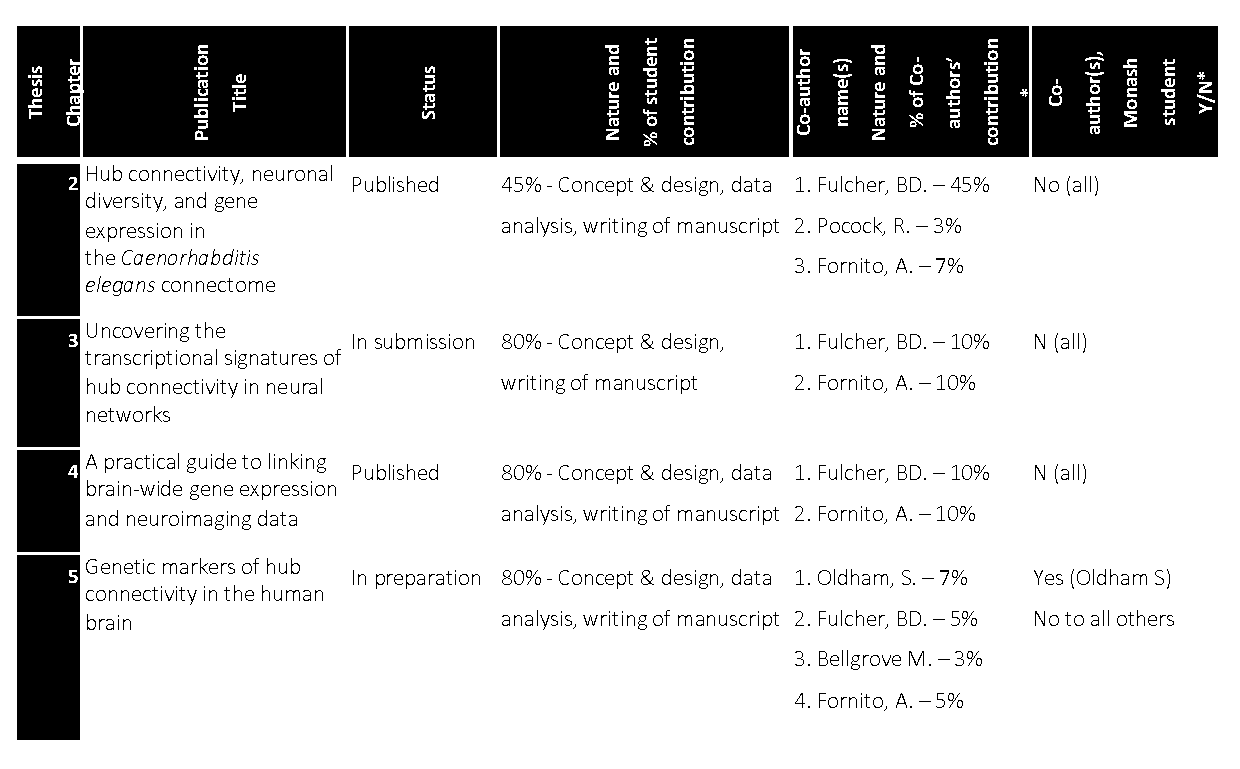
\includegraphics[width=1\textwidth]{declarationTable.pdf}
\label{declaration}
\end{figure}

\newpage
I have renumbered sections of submitted or published papers in order to generate a consistent presentation within the thesis.\\

Student signature:

\includegraphics[height=5em, right]{AAsignature.png}


Date: 14/03/2019\\

The undersigned hereby certify that the above declaration correctly reflects the nature and extent of the student's and co-authors' contributions to this work. In instances where I am not the responsible author I have consulted with the responsible author to agree on the respective contributions of the authors.\\


Main Supervisor signature:

\includegraphics[height=5em]{AFsignature.pdf}

Date: 14/03/2019\\

 \clearpage \thispagestyle{empty} \cleardoublepage 

  \tableofcontents% \clearpage \thispagestyle{empty} 

  \mainmatter

  \fancyhead{}
  \pagestyle{fancy} % headings

  %!TEX root = ../Thesis.tex
\chapter{Introduction}
\label{ch:Introduction}
\fancyhead[R]{\textit{Chapter.} \textit{\thechapter: }\textit{Introduction}}

Brain connectivity forms the anatomical substrate for our consciousness, thoughts, experiences and emotions. Attempts to understand how the network of connections comprising the brain is organised began over a century ago by visualising individual neurons and observing their connectivity patterns \citep{RamonyCajal1995}. Recent developments in brain imaging techniques have enabled researchers to comprehensively examine neuronal connectivity across the entire brain, with a major focus of XXI century neuroscience being on uncovering key properties of brain network organization in both health and disease \citep{VandenHeuvel2010b,Bullmore2012,Fornito2015}.

Understanding the factors that sculpt brain network architecture is essential for future developments in both theoretical and clinical neuroscience. Brain connectivity, like most phenotypes, is the product of myriad environmental and genetic influences. The precise degree to which genes or environment influence distinct aspects of neural structure and function remains a topic of ongoing investigation. The past two decades of brain network research have identified a series of non-trivial properties that are highly conserved across species and resolution scales, from the level of individual neurons and synapses to the macroscale organization of the entire brain, suggesting that such connectivity patterns result from common selection pressures which may, at least in part, be encoded in the genome.

This thesis focuses on understanding genetic contributions to one such property -- connectivity between network hubs. Hubs are neural elements  characterised by a high degree of connectivity to other areas \citep{VandenHeuvel2013b}. They also tend to preferentially connect to each other, forming a putative core of the network and playing a central role in brain communication \citep{VandenHeuvel2011,VandenHeuvel2013a}. Disruptions in connectivity and functioning of hub regions have been associated with a range of neurological and psychiatric disorders \citep{Crossley2014,VandenHeuvel2013b,Fornito2015}. Therefore, studying the genetic properties of hub connectivity can help uncover the molecular mechanisms behind brain network organisation in both health and disease. The remainder of this chapter provides a brief overview of the current research in brain connectivity and the main approaches used to investigate the genetic contributions towards the brain organisation, before outlining the general structure of the thesis.


\section{The brain as a network}
The human brain contains around $86$ billion neurons connected by around $100$ trillion synapses \citep{Williams1988,Andersen1992,Pelvig2008}, forming one of the most complex systems that we know. It is now universally accepted that the brain is comprised of discrete cells interconnected by synaptic junctions -- the so-called neuron doctrine, first proposed in 1894 by Santiago Ram\'{o}n y Cajal \citep{RamonyCajal1995} and later confirmed in the 1950s with the development of the electron microscopy \citep{DeRobertis1955}. This doctrine established a foundation for the modern understanding of the nervous system as a network of discrete, interconnected elements.

Another important observation by Ram\'{o}n y Cajal was that the extraordinary complexity of neuronal organization may be explained by some simple underlying principles. Specifically, he proposed that:
\bigskip
\bigskip

\textit{`` ... all of the various conformations of the neuron and its various components are simply morphological adaptations governed by laws of conservation for time, space and material''}

\hspace{7.5cm}Santiago Ram\'{o}n y Cajal (1995), p.116, Volume I.
\bigskip
\bigskip

Under these laws, neurons and their processes are organised in order to minimise axonal wiring cost, saving both cellular material and intracranial volume, and to minimize conduction delays in the transmission of information between neurons, which requires an efficient configuration of network connectivity. Numerous studies since have supported an important role for conservation of space and material, often operationalized as axonal wiring cost, showing that it can explain microscale properties such as the geometry of neuronal arbors \citep{Cherniak1999} and axonal connection volume \citep{Chklovskii2002}, as well as macroscale features such as the placement of cortical areas \citep{Cherniak2004}. However, due to limitations on available data, these studies focused on restricted sections of tissue or incomplete connectivity, which offers only a partial insight into the general principles of brain network organization.

Developments in microscopy, axonal tract tracing, and non-invasive imaging techniques have led to the emergence of increasingly more precise and detailed connectivity maps in different species \citep{Bota2015,Chiang2011a,Oh2014,Scannell1999,Shanahan2013,Stephan2001,VanEssen2013,White1986}. Such maps range from the microscale connectivity at the level of individual neurons, a regional connectivity at the mesoscale, to the large-scale brain connectivity of the human brain. The creation of the first detailed wiring diagrams of the whole nervous system started with serial electron microscope reconstructions of the hermaphrodite nematode \textit{C.elegans} \citep{White1986}, later supplemented by additional experiments \citep{Varshney2011} resulting in the first full neuronal connectivity network defined at the level of individual neurons and synapses. Consisting of 279 neurons connected by 890 gap junctions, 6393 chemical synapses and 1410 neuromuscular junctions, the somatic nervous system of \textit{C.elegans} serves as a model network for the investigation of the microscale connectivity. In addition to the relatively simple wiring diagram of the \textit{C.elegans}, detailed interregional connectivity maps of the \textit{Drosophila} fly brain have been constructed based on the neuronal connectivity of approximately \num{12000} neurons resulting in a first representative neuronal map of a more complex brain \citep{Chiang2011a}.

Recently, brain mapping investigations have expanded to yield the full connectivity maps of the larvae nervous system \citep{Ohyama2015} and the complete volume of the adult Drosophila brain \citep{Zheng2018}. Reconstructing whole-brain connectivity in larger animals predominantly involves tracing axonal projections between brain areas. Using such methods, inter-regional connectivity maps have been constructed for a range of species including pigeon \citep{Shanahan2013}, mouse \citep{Oh2014}, cat \citep{Scannell1995}, and macaque \citep{Harriger2012}. Investigations of the large-scale connectivity within the human brain rely on non-invasive imaging techniques. Combining diffusion weighted imaging (DWI) with tractography algorithms \citep{Jbabdi2011} enable the reconstruction of the white matter pathways linking macroscopic brain regions. Despite uncertainties associated with the interpretation of the diffusion MRI signal and limitations in tract reconstruction \citep{Jones2010,Jones2013,Thomas2014}, DWI remains the most widely adopted technique to assess structural brain connectivity in human.

Across these diverse species, measurement techniques and spatial resolutions, the resulting comprehensive maps of connectivity are called connectomes, and are typically represented as matrices displaying all pairwise anatomical connections between neural elements (e.g., neurons, cell populations or regions) of the brain \citep{Sporns2005}. The emerging field of connectomics is focused on understanding system-wide patterns of network structure that combined with the dynamics have yielded a more complete picture of the brain. It suggests that a simple cost minimization principle alone may be insufficient to explain neuronal organization.

\section{Topological organisation of the brain}

A central tenet of connectomics is that the brain, like any other network, can be represented as a network of nodes (elements in a network) connected by edges (connections between elements). This general, yet comprehensive way of rendering a network allows investigation of both connectivity --- the presence or absence of connections, and topology --- the precise arrangement of connections between nodes or, more formally, properties of the network that are invariant to its layout in physical space, using the mathematics of graph theory \citep{Barabasi2016}.

Initial studies of brain network topology showed that the brain resembles a small-world architecture \citep{Bassett2006,Gygi1999,Hilgetag2004,Sporns2004,Watts1998} that is characterized by highly clustered, tightly connected subsets of nodes similar to a lattice, combined with sparse long-range projections. Those long-distance connections have been implicated in reducing the topological distance within the network \citep{Bullmore2012,Sporns2004,VandenHeuvel2011} and demonstrated to increase network robustness and promote complex brain dynamics \citep{Betzel2018}. Several other studies have since shown a range of more complex topological properties including a hierarchical community structure of densely connected sub-networks, called modules, such that modules contain nested sub-modules over several resolution scales \citep{Bullmore1997,Meunier2010a,Towlson2013} that are thought to support functional specialization. Furthermore, connectivity across nervous systems is non-uniformly distributed, such that a relatively small number of nodes possess a disproportionately high number of connections, thus representing network hubs \citep{Towlson2013,VandenHeuvel2011}.

The emergence of many of these properties can be explained in the context of Cajal's conservation laws \citep{RamonyCajal1995}. For example, the tendency of neural elements to form connections with spatially proximal neighbours, resulting in anatomically localised communities, is consistent with a cost minimisation rule: geometric constraints of the system favour the formation of short-range connections facilitating the emergence of functionally specialised processing units while penalising biologically expensive long-range projections. In fact, simple generative brain network models based on the exponential decay rule have shown success in recreating networks many topological features that mimic the brain \citep{Ercsey-Ravasz2013,Henderson2014}. The only rule in such models states that connection probability is exponentially decreasing with increasing separation distance between network elements. However, several considerations indicate that this constraint alone is insufficient to explain brain connectivity, as long-range projections occur more frequently than predicted by a simple distance-dependent wiring rule. Introducing additional terms that balance cost minimization with a preference for certain adaptive topological properties, such as forming links between elements that connect to similar nodes, leads to a more accurate model of connectome organization \citep{Betzel2016,Vertes2012}. Such results are in line with a trade-off initially implied by Cajal's conservation laws, in that the pressure to minimize wiring costs must be balanced with the need to promote functionally adaptive topology \citep{Bullmore2012}.

\section{The role of brain network hubs}

Hub connectivity appears to play a major role in how the brain negotiates the trade-off between cost minimization and adaptive topology. Hubs are usually identified using a measure called node degree, which quantifies the number of connections attached to a particular node. In addition to being highly connected, hubs also demonstrate denser interconnectivity between each other than expected by chance forming a so-called ``rich-club'' \citep{Fulcher2016,Harriger2012,Towlson2013,VandenHeuvel2011,Zamora-Lopez2010}. By linking hubs that are distributed throughout the brain, the rich-club forms a biologically costly backbone of the connectome that mediates a high proportion of communication traffic \citep{VandenHeuvel2012,Misic2014}. Rich-club organization is conserved across different species and resolution scales, including the neuronal connectome of the \textit{C.elegans} \citep{Towlson2013}, the mesoscale connectomes of the mouse \citep{Oh2014,Fulcher2016}, cat \citep{DeReus2013b}, macaque \citep{Harriger2012}, and the macroscale connectivity of the human brain \citep{VandenHeuvel2011}, suggesting that it arises from common selection pressures operating on these nervous systems.

As the connections between hubs extend over long anatomical distances \citep{Fulcher2016,Towlson2013,VandenHeuvel2011}, their judicious placement is critical to ensure that their substantial biological costs are offset by the functional advantages they confer \citep{DeReus2014,Towlson2013}. Consistent with this view, hubs of the human brain typically reside in precuneus, insular, anterior and posterior cingulate, superior frontal, lateral parietal and temporal cortices \citep{Gong2009,VandenHeuvel2012,VandenHeuvel2013a} -- areas of paralimbic and association cortex that are known to mediate complex brain function \citep{Buckner2009,Mesulam1998}. Individual differences in hub connectivity are linked to intelligence \citep{Li2009,VandenHeuvel2009}, cognitive task performance \citep{Cole2012}, and personality traits \citep{Adelstein2011}. Furthermore, axonal connections between hub regions have been shown to occupy high white matter volume and exhibit high levels of white matter organization, as quantified by increased fractional anisotropy, a measure that is thought to reflect relative axonal fiber density, diameter and myelination in white matter \citep{Collin2014}. These properties might indicate several advantages associated with increased communication efficiency and robustness along those paths \citep{Collin2014}. Increased involvement of hubs in cognitive processing \citep{Buckner2009,Cole2012,Mesulam1998} together with costly biological attributes are likely to impose increased metabolic demands on those regions \citep{Collin2014}. Indeed, studies of cerebral blood flow and metabolic activity indicate that hub regions are among the most metabolically active areas \citep{Vaishnavi2010,Varkuti2011}.

As argued by Bullmore and Sporns \citep{Bullmore2012}, it is intuitive to expect that an impact on a topologically central area will result in the greatest disruption, as affected hubs have a disproportionate effect on the integrative capacity of the brain \citep{DeReus2014}. Indeed, converging evidence suggests that hubs are more susceptible to a diverse range of diseases \citet{Bassett2009a,Crossley2014,Fornito2015}. The topologically central position of hubs means that they can be easily affected by a disruption originating elsewhere in the brain \citep{Zhou2012}. Moreover, many connections involving hubs extend over long distances \citep{VandenHeuvel2012}, hence increasing their susceptibility to injury. For instance, schizophrenia patients demonstrate both structural and functional changes, including reduced frontal hub connectivity \citep{Fornito2012a,VandenHeuvel2010,Zalesky2011} and disrupted rich-club formation \citep{VandenHeuvel2013c}. Aging studies have also identified hub connectivity changes in Alzheimer’s disease \citep{DeHaan2012,Stam2009} and frontotemporal dementia \citep{Agosta2013}. Moreover, changes in hub organization \citep{Achard2012} and metabolic activity \citep{Laureys2004} have been associated with reduced consciousness states. Together these findings demonstrate the involvement of hubs in a broad range of disorders and highlight their importance in normal brain functioning.

The emergence of hubs and rich-club connectivity across multiple species points to a strong conservation across the evolutionary tree, which may result from a general selection pressure to maintain adaptive performance at low metabolic cost \citep{Bullmore2012}. A corollary of this view is that hub connectivity is a strong candidate for higher then average genetic control. Given the importance of hubs in brain function, an investigation into the genetics of hub connectivity is likely to have important implications for understanding the molecular basis of both behaviour and disease.
\section{Genetic markers of brain connectivity}

Genetic influences on human brain networks have typically been examined using one of three primary methods: i) quantifying the degree of genetic control over a trait through heritability analysis; ii) identifying associations between trait variability and allelic variation of structural DNA at the level of single nucleotide polymorphisms (SNPs); iii) or investigating how anatomical variations of a given network property correlate with the spatial patterning of gene expression.

\subsection{Heritability}

Twin studies offer a natural experiment that allows researchers to quantify the heritability of a trait, i.e., the proportion of trait variance that is attributable to genes. They rely on the assumption that monozygotic (MZ) twins share all of their genetic information whereas dizygotic (DZ) twins, on average, have $50\%$ of their genes in common. Under the further assumption that environmental contributions affect both twin groups to a similar extent, structural equation modelling can be used to partition phenotypic variability into proportions of variance explained by common environment (non-genetic influences shared between members of a twin pair), unique environment (person-specific experiences and measurement error), and genetic influences. Generally, overall heritability of the trait entails the effect of additive, dominant and genetic interaction contributions, together termed the \textit{broad-sense heritability}. In the context of imaging genetic studies, heritability estimates are traditionally modelled to reflect a proportion of the total variance that is attributable to the additive allelic effects, termed the \textit{narrow-sense heritability}. Thus, a heritability, $h^{2}$, of zero indicates no genetic contributions to the trait, whereas $h^{2}=1$ implies that all trait variation between people is explained by genetic factors.

Heritability has been widely adopted in the context of brain imaging. Twin studies of brain structure have shown strong genetic influences over global properties such as the total grey and white matter volume
\citep{Baare2001,Bohlken2014,Wright2002} and whole-brain microstructural integrity as quantified using fractional anisotropy \citep{Bohlken2014}. More specifically, inter-hemispheric tracts demonstrate increased heritability \citep{Shen2014,Sudre2017} compared to more local intra-hemispheric connections. Paralleling these structural data, genetic influences have also been found using various fMRI measures of functional connectivity \citep{Colclough2017} \citep{Fu2015,Glahn2010,Sudre2017} and specific topological properties in structural \citep{Bohlken2014} and functional \citep{Fornito2011,Sinclair2015}  networks. Measures associated with both cost minimisation (modularity, clustering coefficient) as well as efficient information transfer (global efficiency, characteristic path length, small-worldness) demonstrate significant genetic contributions \citep{Sinclair2015,Bohlken2014}. These findings support the general assumption of genetic control over establishing effective communication while maintaining constraints on wiring cost. Integrating both cost minimisation and communication efficiency into a single measure of network cost-efficiency, substantial genetic effects have been demonstrated in human functional connectivity networks \citep{Fornito2011}. Critically, brain regions showing significant heritability of cost-efficiency were located in the areas of paralimbic and association cortex, implying that network hubs comprise a genetically determined core of both structural and functional connectivity that facilitates efficient communication at relatively low cost.

Twin design is an attractive and informative concept for investigating genetic contributions, however it also poses some limitations. For example, the equal environment assumption underlying heritability models has been disputed  \citep{Charney2017,Joseph2002}, since the shared prenatal environment differs between MZ and DZ twin pairs [e.g., MZ twins experience higher stress due to sharing a single placenta and outermost fetal membrane \citep{Corsello2010}] and MZ twins are treated more similarly later in life than DZ twins \citep{Joseph2002}. Moreover, differences in mitochondrial DNA and nuclear genome copy number variations mean that MZ twins are not $100\%$ genetically identical \citep{Bruder2008,Charney2017}. In addition, the estimation of genetic effects is contingent on population-level exposure. As a result, heritability estimates derived from twin studies are often regarded as inflated whereas the environmental contributions are likely to be consistently underestimated \citep{Joseph2002}. Despite these limitations, heritability remains a useful starting point to quantify genetic contributions to a trait.

\subsection{Structural DNA variation}

While heritability quantifies the proportion of trait variance attributable to genes, it does not provide information about which specific genetic variants may be involved. Such variants are typically identified using linkage and association analyses \citep{Thompson2013}. Linkage analyses exploit inheritance patterns within families and aim to determine the co-segregation of the genotype and phenotype across individuals. Association analyses test for associations between the trait and allelic variation at different points  throughout the genome. The most comprehensive form of such analysis tests millions of markers scattered throughout the genome and is called a genome-wide association study (GWAS). Candidate gene studies, on the other hand, apply a hypothesis-driven approach by genotyping and testing markers that are hypothetically linked to a trait.

Some of the first studies linking DNA variants to brain connectivity used a candidate gene approach by testing theoretically or experimentally derived hypotheses [for a review see \citet{Thompson2013}], and found associations with a range of brain connectivity phenotypes, including white matter microstructure \citep{Braskie2012,Chiang2011,Jahanshad2012b}, topological network properties \citep{Dennis2011}, and resting state functional connectivity \citep{Filippini2009,Trachtenberg2012,Westlye2011}. However, candidate gene studies have been called into question due to relatively high chance of false positives \citep{Sullivan2007} and low replication rate, potentially resulting from population stratification \citep{Hutchison2004}. More recent GWAS analyses have identified variants related to structural connectivity \citep{Chiang2009,Jahanshad2013,Jahanshad2012a} and other imaging phenotypes \citep{Elliott2018}, however these studies require very large samples to achieve sufficient statistical power. Even within the ENIGMA consortium \citep{Thompson2014}, which was formed to address this issue, ensuring consistent quality control across multiple sites remains a challenge.

Considering the polygenic nature of most complex traits, with thousands of common variants contributing only small effect sizes, polygenic scores (PGS) allow quantification of the aggregate impact of multiple SNPs on a given trait \citep{Dudbridge2013}. The PGS is a weighted sum of SNP-specific effect-size estimates for a given trait derived from an independent GWAS. By summing genetic contributions in a single score, it provides greater power for assessing relationships to imaging-derived phenotypes (IDPs), at the expense of the ability to localize the specific variants driving the association. The general utility of PGS in the field of imaging genetics has been questioned \citep{Papiol2014} mostly due to its low predictive power, as PGS can potentially account for only a small proportion of the total phenotypic variance. Although a few large-scale analyses did not identify associations between subcortical volumes and the genetic liability for psychiatric illness \citep{Franke2016,Reus2017}, several studies have found relationships between PGS for different psychiatric disorders and cortical gyrification \citep{Liu2016a}, functional connectivity \citep{Dezhina2018,Wang2017}, and longitudinal changes in white matter properties \citep{Alloza2018}. Some of those findings implicate known connectome hubs such as insula, cingulate and prefrontal cortex [for a review see \citet{Dezhina2018}], supporting the hypothesis that polygenic liability for psychiatric disorders influences functionally and structurally important regions.

\subsection{Gene expression}

The influence of structural DNA variation on a given trait is mediated by the specific way in which those variants impact gene function, but this impact is not immediately obvious when conducting GWAS or candidate gene studies. Particularly in GWAS, putatively causal variants are identified through statistical means, and may not tag the location of the actual causal variant. The development of brain-wide gene expression atlases \citep{Harris2010,Hawrylycz2012,Lein2007a} has opened opportunities for linking gene function to large-scale neural phenotypes measured across the entire brain [for a review see \citet{Fornito2019}]. The process of gene expression consists of multiple stages including transcription, when an unwound segment of DNA is read to produce messenger RNA (mRNA) and translation, when the resulting mRNA is used to synthesize a particular gene product. Gene expression is commonly inferred by quantifying levels of mRNA, which corresponds to transcriptional activity and is an indirect proxy for protein abundance \citep{Liu2016}. In species with high tissue availability, gene expression can be measured at a cellular resolution using methods such as \textit{in-situ} hybridization \citep{Lein2007a,Unger2010}, whereas bulk-tissue microarray \citep{Schulze2001} remains the most accessible method for high-throughput analysis in humans \citep{Hawrylycz2012}. Unlike heritability and structural DNA studies, which examine genetic contributions to phenotypic variability across individuals, atlas-based approaches investigate how spatial patterns of gene expression are related to spatial variations in brain structure or function. This can be achieved by using gene expression measures to evaluate (i) regional gene expression; (ii) correlated gene expression (CGE) between pairs of regions; or (iii) gene coexpression between pairs of genes. Each of those approaches addresses a distinct question: the aim of regional gene expression analyses is to identify associations between regional variations in gene expression and some regional property of the brain, such as node degree \citep{French2011}; CGE quantifies transcriptional coupling between regions across large swathes of the genome and can be related to pairwise properties of brain connectivity such as the presence or absence of a connection or the type of a connection they share \citep{Arnatkeviciute2018,Fulcher2016,Richiardi2015}; gene coexpression analyses focus on the correlations between the regional expression profiles of pairs of genes, thus evaluating which genes have similar expression patterns across the brain \citep{Forest2017}.

Some of the first studies integrating atlas-based gene expression measures with brain connectivity discovered gene expression signatures that are predictive of both neuronal connectivity in \textit{C.elegans} 
\citep{Kaufman2006} and regional connectivity in rodents \citep{Fakhry2015,Fakhry2015a,Ji2014,French2011}. Later, regional gene expression patterns in the human brain were shown to relate to a range of structural and functional properties including the specialisation of brain areas \citep{Anderson2018,Krienen2016,Parkes2017}, structural
\citep{Goel2014} and functional \citep{Cioli2014b,Forest2017,Richiardi2015,Vertes2016b} connectivityn and brain development \citep{Kirsch2016a,Whitaker2016a}. Building on the evidence that the topological properties of hub connections are highly heritable \citep{Fornito2011}, Fulcher and Fornito investigated the transcriptional signatures of hub connectivity in the mouse brain \citep{Fulcher2016}. They demonstrated an elevated transcriptional coupling between spatially distributed hub regions that was primarily driven by genes regulating ATP synthesis and metabolism. These findings point to a molecular signature related to the high metabolic cost and function of hub connectivity \citep{Liang2013a,Tomasi2013}.
Parallel evidence from fMRI in humans indicates that hubs with long-range connections that preferentially connect disparate neural systems may possess a comparable signature involving metabolism-related genes \citep{Vertes2016b} suggesting the existence of a conserved transcriptional signature associated with hub connectivity across species and scales.

\section{Interim summary}

In summary, brain network architecture appears to be driven by a trade-off between minimizing the axonal wiring costs and promoting efficient, adaptive function \citep{Bullmore2012}. Converging evidence suggests that this balance is negotiated in large part through the formation of a densely inter-connected rich-club -- a putative communication backbone of the brain mediating a high proportion of communication traffic \citep{VandenHeuvel2011}. The emergence of hubs and rich-club connectivity across different species and scales points to common evolutionary pressures to maintain effective brain network communication at relatively low cost. These results raise the possibility that such pressures may be at least partly mediated through genes. Despite a growing body of literature demonstrating the genetic influences over brain connectivity, as quantified using heritability, structural DNA analysis [see \citet{Thompson2013} for a review], and brain-wide gene expression [see \citet{Fornito2019} for a review] only a limited number of studies have explicitly focused on the genetic basis of hubs and rich-clubs.

\section{Aims and overview of the thesis}

Following the initial evidence from twin study in humans suggesting a genetic contribution to cost-efficient properties of hub connectivity \citep{Fornito2011}, and the unique transcriptional signature of hub connectivity that may be conserved across mouse and human \citep{Vertes2016b,Fulcher2016}, the broad aim of this thesis is to comprehensively investigate genetic contributions to hub connectivity across different scales and levels of genetic influence. In particular, this thesis focuses on analyses between two disparate scales: the microscale connectome of the nematode \textit{C.elegans} that presents a full wiring diagram at the level of individual neurons and synapses and the macroscale inter-regional connectivity of the human brain. This thesis consists of six chapters, including three peer-reviewed manuscripts (two published, one under review).

\textit{Chapter 2} presents a peer-reviewed paper investigating hub connectivity and gene expression in the \textit{C.elegans} connectome. The goal of this work was to determine whether the transcriptional signature of hub connectivity identified in the mesoscale connectome of the mouse brain \citep{Fulcher2016} could be detected in the neuronal connectome of the \textit{C.elegans} nervous system. The study combines a broad range of publicly available data and demonstrates that, like the mouse, connected pairs of hub neurons of the worm show the most similar patterns of gene expression. This similarity is driven by genes involved in glutamatergic and cholinergic signalling, and other neural communication processes. It also shows that the increased gene expression similarity between hub neurons cannot be explained by a range of neuronal properties such as their subtype, separation distance, chemically secreted neurotransmitter, birth time, pairwise lineage distance, or the topological module affiliation. Instead, this coupling is linked to the functional designation of most hubs as command interneurons, a specific class of interneurons that regulates locomotion.

\textit{Chapter 3} provides a review of the current research investigating the transcriptional signatures of hub connectivity in neural networks across different species and scales including the findings in the \textit{C.elegans} connectome presented in Chapter 2. This manuscript was written as an invited article and currently is under review in the \textit{Frontiers In Neural Circuits}. It focuses specifically on the link between gene expression and hub connectivity and sets the stage for later chapters, that primarily investigate the transcriptional and other genetic properties of hub connectivity in the human brain.

\textit{Chapter 4} entails a peer-reviewed paper focusing on methodological choices involved in integrating publicly available Allen Human Brain Atlas (AHBA) with neuroimaging. A growing number of studies are using the AHBA to map gene expression correlates of various brain imaging phenotypes, but inconsistencies in methods used for processing the AHBA data pose problems for interpretation and reproducibility. This paper introduces a seven-step analysis pipeline for relating AHBA brain-wide transcriptomic and neuroimaging data and compares the influence of different processing choices. This work takes an important first step towards standardized analysis pipeline that can be routinely employed throughout the field. It is a necessary precursor for the analyses of Chapter 5.

\textit{Chapter 5} presents an extensive investigation of the genetic correlates of hub connectivity in the human brain. First, genetic control over the structural brain networks is quantified through the edge-wise, connectome-wide heritability analysis. Second, the effect of structural DNA variation on hub connectivity is examined using polygenic scores for a range of psychiatric disorders and IQ. Finally, the transcriptional correlates of hub connectivity are investigated using AHBA gene expression data. The findings indicate that the strength of connectivity between hubs is the most highly heritable, is related to polygenic liability for mental illness and high IQ, and is characterized by a similar transcriptional signature of hub connectivity observed in mouse -- namely elevated transcriptional coupling predominately driven by metabolic genes. 

Together, these findings establish a link between molecular function and large-scale connectome organization across different species and modalities and demonstrate that genetic influences on neuronal connectivity converge on brain network hubs. The general discussion, limitations and the directions for future research are presented in \textit{Chapter 6}.
 
  \clearpage
  %!TEX root = ../Thesis.tex
\chapter{Hub connectivity and gene expression in \textit{C.elegans}}
\label{ch:Chapter2}
\fancyhead[R]{\textit{Chapter.} \textit{\thechapter: }\textit{Hub connectivity and gene expression in \textit{C.elegans}}}


% Insert author names, affiliations and corresponding author email (do not include titles, positions, or degrees).

\textbf{Aurina Arnatkevi\u{c}i\={u}t\.{e}}*,
Ben D. Fulcher*,
Roger Pocock,
Alex Fornito (2018).
Hub connectivity, neuronal diversity, and gene expression in the \emph{Caenorhabditis elegans} connectome. \textit{PLOS Computational Biology}.
*These authors contributed equally.\\
DOI: \url{https://doi.org/10.1371/journal.pcbi.1005989} % Please use "sentence case" for title and headings (capitalize only the first word in a title (or heading), the first word in a subtitle (or subheading), and any proper nouns).



\section*{Preamble}
Building on the previous work in the mesoscale connectome of the mouse brain, showing that hub regions have a distinct transcriptional signature driven by oxidative metabolism related genes \citep{Fulcher2016}, in this chapter we aimed to test whether hubs in a microscale neuronal connectome demonstrate similar properties. The nervous system of the \textit{C.elegans} worm has been mapped at the level of individual neurons and synapses and constitutes a gold-standard connectivity map. Combining a rich set of publicly available data, we demonstrate, that hub neurons in the \textit{C.elegans} connectome show increased gene expression similarity that cannot be attributed to a wide range of properties including their neuronal subtype, spatial separation distance, chemically secreted neurotransmitter, birth time, pairwise lineage distance, topological module affiliation. Instead it is related to the functional identity of most hub neurons as command interneurons that regulate locomotion. \\ Supplementary materials for this chapter are in Appendix \ref{appendixA}.


\newpage

\section*{Abstract}
Studies of nervous system connectivity, in a wide variety of species and at different scales of resolution, have identified several highly conserved motifs of network organization.
One such motif is a heterogeneous distribution of connectivity across neural elements, such that some elements act as highly connected and functionally important network hubs.
These brain network hubs are also densely interconnected, forming a so-called rich-club.
Recent work in mouse has identified a distinctive transcriptional signature of neural hubs, characterized by tightly coupled expression of oxidative metabolism genes, with similar genes characterizing macroscale inter-modular hub regions of the human cortex.
Here, we sought to determine whether hubs of the neuronal \textit{C.elegans} connectome also show tightly coupled gene expression.
Using open data on the chemical and electrical connectivity of 279 \textit{C.elegans} neurons, and binary gene expression data for each neuron across 948 genes, we computed a correlated gene expression score for each pair of neurons, providing a measure of their gene expression similarity.
We demonstrate that connections between hub neurons are the most similar in their gene expression while connections between nonhubs are the least similar.
Genes with the greatest contribution to this effect are involved in glutamatergic and cholinergic signaling, and other communication processes.
We further show that coupled expression between hub neurons cannot be explained by their neuronal subtype (i.e., sensory, motor, or interneuron), separation distance, chemically secreted neurotransmitter, birth time, pairwise lineage distance, or their topological module affiliation.
Instead, this coupling is intrinsically linked to the identity of most hubs as command interneurons, a specific class of interneurons that regulates locomotion.
Our results suggest that neural hubs may possess a distinctive transcriptional signature, preserved across scales and species, that is related to the involvement of hubs in regulating the higher-order behaviors of a given organism.

\section*{Author summary}

Some elements of neural systems possess many more connections than others, marking them as network hubs.
These hubs are often densely interconnected with each other, forming a so-called rich-club that is thought to support integrated function.
Recent work in the mouse suggests that connected pairs of hubs show higher levels of transcriptional coupling than other pairs of brain regions.
Here, we show that hub neurons of the nematode \textit{C.elegans} also show tightly coupled gene expression and that this effect cannot be explained by the spatial proximity or anatomical location of hub neurons, their chemical composition, birth time, neuronal lineage or topological module affiliation.
Instead, we find that elevated coexpression is driven by the identity of most hubs of the \textit{C.elegans} connectome as command interneurons, a specific functional class of neurons that regulate locomotion.
These findings suggest that coupled gene expression is a highly conserved genomic signature of neural hubs that may be related to the specific functional role that hubs play in broader network function.

%% main text
\section{Introduction}
\label{sec:introduction_ch2}

Neuronal connectivity provides the substrate for integrated brain function.
Recent years have seen several systematic and large-scale attempts to generate comprehensive wiring diagrams, or connectomes, of nervous systems \citep{VandenHeuvel2016} in species as diverse as the nematode \emph{Caenorhabditis elegans} \citep{White1986, Varshney2011}, \emph{Drosophila} \citep{Chiang2011a, Shih2015}, zebrafish \citep{Wanner2016, Hildebrand2017}, mouse \citep{Oh2014, Zingg2014}, rat \citep{Bota2015}, cat \citep{Scannell1995}, macaque \citep{Markov2014, Stephan2001}, and human \citep{Hagmann2008, VanEssen2013}.
One of the most striking findings to emerge from analyses of these diverse data, acquired using different measurement techniques and at resolution scales ranging from nm to mm, is of a strong conservation of certain topological properties of network organization [reviewed in \citep{Bullmore2009, Bullmore2012, Sporns2011, VandenHeuvel2016b, Schroter2017}, see also \citep{Fornito2016}].
These properties include a modular organization, such that subsets of functionally related (and usually spatially adjacent) elements are densely interconnected with each other;
a hierarchy of modules, such that modules contain nested sub-modules and so on over multiple scales \citep{Meunier2010a, Bassett2010};
economical connectivity, such that wiring costs (typically measured in terms of wiring length) are near-minimal given the topological complexity of the system \citep{Betzel2016, Bassett2010};
a heterogeneous distribution of connections across network nodes, such that most nodes possess relatively few connections and a small proportion of nodes have a very high degree of connectivity \citep{VandenHeuvel2013b, Varshney2011};
and stronger interconnectivity between hub nodes than expected by chance, leading to a so-called rich-club organization [i.e., the hubs are rich because they are highly connected and form a club because they are densely interconnected \citep{VandenHeuvel2011,Zamora-Lopez2010,DeReus2013b,Towlson2013,Shih2015}].

The rich-club organization of hub connectivity is thought to play a central role in integrating functionally diverse and anatomically disparate neuronal systems \citep{Fornito2015,VandenHeuvel2013a,Zamora-Lopez2010, Crossley2014,Crossley2013}. Consistent with this view, experimental data and computational modeling indicates that hub nodes, and the connections between them, are topologically positioned to mediate a high volume of signal traffic \citep{VandenHeuvel2012, Harriger2012, Misic2014, Misic2015a}.
This integrative role comes at a cost, with connections between hubs extending over longer distances, on average, than other types of connections, a finding reported in the human \citep{VandenHeuvel2012}, macaque \citep{Harriger2012}, rat \citep{VandenHeuvel2016b}, mouse \citep{Fulcher2016}, and nematode \citep{Towlson2013}.
Human positron emission tomography also suggests that hub nodes consume greater metabolic resources and have higher levels of blood flow than other areas \citep{Tomasi2013, Collin2014, Liang2013a}.
This high metabolic cost may underlie the involvement of hub regions in a broad array of human diseases \citep{Fornito2015, Bullmore2012, Crossley2014}.

Recent studies in mice and humans suggest that the high cost of hub connectivity is associated with a distinct
molecular signature, as inferred from brain-wide transcriptomic data.
This work has focused on how patterns of expression across many thousands of genes covary between pairs of brain regions.
Such patterns of covariation are variously referred to as transcriptional coupling \citep{Fulcher2016}, gene coexpression \citep{Krienen2016} or correlated gene expression \citep{Richiardi2015, Mills2018, Goel2014}.
The goal of this work is to understand how pair-wise coupling of gene expression corresponds to the pairwise connection topology of the brain, thus drawing a link between molecular function and large-scale network organization.
For example, Fulcher and Fornito \citep{Fulcher2016} combined viral tract tracing data on connectivity between 213 regions of the right hemisphere of the mouse brain \citep{Oh2014} with \emph{in situ} hybridization measures of the expression of \num{17642} genes in each of those regions.
They found that transcriptional coupling, across all genes, is stronger for connected compared to unconnected brain regions and that, in general, this coupling decays with increasing separation distance between brain regions.
Countering this general trend, however, connected pairs of hubs (i.e., the ``rich club'' of the brain) show the highest levels of transcriptional coupling (compared to hub-nonhub and nonhub-nonhub pairs), despite being separated by larger distances, on average, and being distributed across diverse anatomical brain divisions.
Moreover, this coupling is driven predominantly by genes regulating the oxidative synthesis and metabolism of adenosine triphosphate (ATP), the primary energetic currency of neuronal signaling \citep{Lennie2003, Laughlin2003}. \citet{Vertes2016b} later combined gene expression data of \num{20737} genes through 285 cortical areas of the human brain and found evidence that inter-modular hubs in resting state fMRI connectivity networks also have local transcriptional profiles enriched in oxidative metabolism and mitochondria.

Together, the analyses of \citet{Fulcher2016} and \citet{Vertes2016b}, which were performed using measures of mesoscale ($\mu$m to mm) and macroscale (mm to cm) connectivity, respectively, suggest that the molecular signature of hub connectivity, characterized by elevated coupling of genes regulating oxidative metabolism, may be conserved across species and resolution scales.
Here, we sought to test this hypothesis by examining the link between gene expression and microscale connectivity in the nematode \emph{C.elegans}.
\emph{C.elegans} is the only species to have its connectome mapped almost completely at the level of individual neurons and synapses using electron microscopy \citep{White1986, Varshney2011}.
It comprises 302 neurons and around 5600 chemical and electrical synapses \citep{White1986}.
We combined these data on neuronal connectivity with curated information on the binary expression patterns of 948 genes across neurons to examine the relationship between gene expression and the large-scale topological organization of the nematode nervous system.
We also used detailed information on neuron spatial positions, birth times, neuronal lineage as well as the functional and chemical composition of each neuron to understand the mechanisms through which gene expression might influence network topology.
Paralleling findings in humans and mouse, we find that hub neurons of \emph{C.elegans} are genomically distinct, with connected hub neurons showing the most similar patterns of gene expression.
Genes that contribute most to this effect are involved in regulating glutamate and acetylcholine function, and neuronal communication.
We demonstrate that this effect cannot be explained by factors such as neuronal birth time, lineage, neurotransmitter system or spatial position, but may instead be related to the functional specialization of hub neurons in mediating higher order behaviours of the organism.

\section{Materials and methods}
\label{Ch2Methods}

We first describe the neural connectivity data used to construct a connectome for \textit{C.elegans} and the methods used to quantify network connectivity and other properties of individual neurons, including their neurochemical composition, birth times, and lineage relationships.
We then describe the gene expression data, how we measure expression similarity between pairs of neurons, and our method for scoring the contribution of individual genes to patterns of correlated gene expression.
Note that all data used for analysis in this work were obtained from publicly available sources, and can be downloaded from an accompanying figshare repository (\url{figshare.com/s/797199619fbabdab8c86}).
Code to process this data and reproduce all figures and analyses presented here is on github (\url{github.com/BMHLab/CElegansConnectomeGeneExpression}).

\subsection*{Neuronal connectivity data}
The nervous system of \emph{C.elegans} comprises 302 neurons, divided into the pharyngeal nervous system (20 neurons) and the somatic nervous system (282 neurons).
While research detailing the genetic underpinnings that guide the formation of \textit{C.elegans} nervous system is still ongoing, the spatial positions of neurons, and their interconnections, are known to be stereotypical across organisms \citep{Riddle1997}.
Neuronal connectivity data for the adult hermaphrodite \emph{C.elegans} was first mapped by \citet{White1986} through detailed electron microscopy, and then revised by \citet{Chen2006} and \citet{Varshney2011}.
Here we analyze the larger somatic nervous system using data from \citet{Varshney2011}, who mapped connectivity between 279 neurons (282 somatic neurons, i.e., excluding CANL/R, and VC6, which do not form synapses with other neurons), which we obtained from WormAtlas \citep{WormAtlas} (\url{www.wormatlas.org/neuronalwiring.html#NeuronalconnectivityII}).

Connectivity data are available for both electrical gap junctions and chemical synapses.
The chemical synapse network is both directed (i.e., the pre-synaptic and post-synaptic neurons are identified) and weighted (as the number of synapses from one neuron to another), while gap junctions are conventionally represented as weighted (as the number of electrical synapses connecting two neurons), undirected connections.
Previous investigations of \emph{C.elegans} neuronal connectivity have used differently processed versions of these data, including:
(i) only chemical synapses \citep{Kashtan2004};
(ii) a combination of chemical and electrical synapses as a directed network (electrical synapses represented as reciprocal connections) \citep{Azulay2016, Kim2016};
(iii) a combination of chemical and electrical synapses as an undirected network (representing unidirectional and reciprocal chemical connections equivalently) \citep{Towlson2013, Kim2014a, Pavlovic2014, Demesmaeker2017};
or (iv) comparing multiple connectome representations \citep{Pan2010}.

Our analysis here focuses on the combined directed, binary network, treating gap junctions as bidirectional connections.
We chose to focus on a binarized network to follow previous studies on \textit{C.elegans} connectome data \citep{Kaufman2006, Towlson2013, Varier2011, Varadan2006, Pavlovic2014} and to enable a more direct comparison to our previous analysis of the relationship between (binary) connectivity and gene expression in mouse \citep{Fulcher2016}.
The resulting connectome contains 279 neurons, with \num{2990} unique connections linking \num{2287} pairs of neurons.

Note that the qualitative results presented here are not highly sensitive to the types of connections included in the connectome.
For example, neuron degree is highly correlated between networks generated using: (i) combined chemical and electrical synapses and (ii) chemical synapses only (Spearman's $\rho= 0.9$, $p = 3 \times 10^{-107}$).
We also obtained qualitatively similar results for rich-club organization and trends in CGE when excluding gap junctions from our analysis (see Figure \ref{fig:Ch2S1_Fig}).

In addition, we assembled a range of data characterizing other properties of \emph{C.elegans} neurons.
To examine the effect of physical distance between pairs of neurons, we obtained two dimensional spatial coordinates for each neuron as \texttt{celegans277.mat} from \url{www.biological-networks.org/?page_id=25} \citep{Choe2004}.
Coordinates for three neurons (AIBL, AIYL, SMDVL) were missing in this dataset, and were reconstructed by assigning identical coordinates to the corresponding contralateral neurons (AIBR, AIYR, SMDVR) \citep{Varier2011}.
To examine the influence of anatomical location, each neuron was labeled by its anatomical location, as:
(i) `head', (ii) `tail', or (iii) `body', using data from release WS256 of WormBase \citep{Harris2010}, (\url{ftp://ftp.wormbase.org/pub/wormbase/releases/WS256/ONTOLOGY/anatomy_association.WS256.wb}).
These annotations were assigned to individual neurons using the anatomical hierarchy defined in WormBase, which we retrieved using the WormBase API (WormMine: \url{intermine.wormbase.org}) \citep{Harris2010}, propagating each term down the hierarchy to individual neurons.
We manually corrected the assignment of twelve head neurons (ALA, AVFL, AVFR, AVG, RIFL, RIFR, RIGL, RIGR, SABD, SABVL, SABVR, SMDVL), which were assigned as `head' in WormAtlas \citep{WormAtlas} but not on WormBase.
To examine the influence of neuronal subtype, all neurons were labeled to one (or multiple) of the following three categories:
(i) `sensory' (have clear sensory specializations),
(ii) `motor' (make synaptic contacts onto muscle cells), or
(iii) `interneuron' (receive synapses from and send synapses onto other neurons) \citep{White1986}.
A total of 79 neurons are annotated as sensory, 121 annotated as motor, and 97 annotated as interneurons (including eighteen neurons assigned to two categories: five are both `interneuron' and `sensory', seven are `interneuron' and `motor', and six are both `sensory' and `motor' neurons).
To examine the neurotransmitter systems used by each neuron, neurons were labeled by matching to Table 2 of \citet{Pereira2015}.
In order to determine the influence of neuron birth time, we obtained neuronal birth time information in minutes from the Dynamic Connectome Lab website (\url{https://www.dynamic-connectome.org/?page_id=25}), \citep{Varier2011}.
To assess the influence of lineage similarity, we obtained a measure of lineage distance for all pairs of neurons from previously published embryonic and post-embryonic lineage trees \citep{Sulston1977, Sulston1983}, using data downloaded from WormAtlas (\url{http://www.wormatlas.org/neuronalwiring.html#Lineageanalysis}) \citep{WormAtlas}.
In this dataset, the closest common ancestor neuron was identified for each pair of neurons, and then the lineage distance was calculated as the number of cell divisions from the closest common progenitor neuron.

\subsection*{Network analysis}
In this section we describe the network analysis methods used to characterize the \emph{C.elegans} connectome.

\paragraph{Degree.}
Neuronal connectivity is most simply quantified by counting the number of neurons that a given neuron projects to, known as its out-degree, $k_\mathrm{out}$, or by counting the number of neurons that a given neuron receives projections from, known as its in-degree, $k_\mathrm{in}$.
These quantities can be summed to give the total number of connections involving a given neuron, $k_\mathrm{tot} = k_\mathrm{in} + k_\mathrm{out}$, which we refer to as simply the degree, $k$, throughout this work.
At a given degree threshold, $k$, each neuron was classified as either a `hub' (degree $>k$) or a `nonhub' (degree $\leq k$).
All connections were subsequently classified in terms of their source and target neurons as either
`rich' (hub $\rightarrow$ hub, or hub $\leftrightarrow$ hub),
`feed-in' (nonhub $\rightarrow$ hub),
`feed-out' (hub $\rightarrow$ nonhub),
or `peripheral' (nonhub $\rightarrow$ nonhub, or nonhub $\leftrightarrow$ nonhub).

\paragraph{Rich-club organization.}
We used the rich-club coefficient, $\phi(k)$, to quantify the interconnectivity of hub neurons:
\begin{equation}
    \label{eqn:rich_club}
    \phi(k) = \frac{2E_{>k}}{N_{>k}(N_{>k}-1)},
\end{equation}
where $N_{>k}$ is the number of nodes with degree $>k$, and $E_{>k}$ is the number of edges between them \citep{Colizza2006}.
Thus, $\phi(k)$ measures the link density in the subgraph containing nodes with degree $>k$.
Because $\phi(k)$ invariably increases with $k$ (as nodes with higher degree make more connections, yielding a higher expected link density in the subgraph containing nodes with degree $>k$), we compared $\phi(k)$ measured from the \emph{C.elegans} connectome to the mean value of an ensemble of randomized null networks, $\phi_\mathrm{rand}(k)$ \citep{Colizza2006}.
An ensemble of 1000 null networks was generated by shuffling the links in the empirical network while retaining the same degree sequence \citep{Maslov2002} (rewiring each edge an average of 50 times per null network) using the \texttt{randmio\_dir} function from the Brain Connectivity Toolbox \citep{Rubinov2010}.
The normalized rich-club coefficient, $\Phi_\mathrm{norm}(k)$, was computed as the ratio of the rich-club coefficient of the empirical network to the mean rich-club coefficient of the ensemble of randomized networks:
\begin{equation}
    \label{eqn:rich_club_norm}
    \Phi_\mathrm{norm}(k) = \frac{\phi(k)}{\langle \phi_\mathrm{rand}(k) \rangle}.
\end{equation}
Values of $\Phi_\mathrm{norm} > 1$ indicate rich-club organization of the network, with statistically significant deviations assessed by computing a $p$-value directly from the empirical null distribution, $\phi_\mathrm{rand}(k)$, as a permutation test \citep{VandenHeuvel2011}.

\paragraph{Modularity.}
Another important topological property of neural systems is modularity, whereby network nodes coalesce into tightly connected subsystems that are thought to serve a common function \citep{Sporns2016}.
To investigate whether our results were influenced by the well-known modular organization of the \emph{C.elegans} connectome \citep{Kim2014a, Pan2010, Bassett2010, Achacoso1992, Pavlovic2014}, we decomposed the network into modules using two methods.
The first method involved applying the Louvain community detection algorithm \citep{Blondel2008} using the \texttt{community\_louvain} function in the Brain Connectivity Toolbox \citep{Rubinov2010}.
To identify the optimal modular assignment, neurons were assigned to modules using consensus clustering across 1000 repeats of the Louvain algorithm \citep{Lancichinetti2012}, weighting each partition by its modularity, $Q$, using the \texttt{agreement\_weighted} and \texttt{consensus\_und} functions of the BCT \citep{Rubinov2010}.
The second modular decomposition was taken from a previously-reported nine-module partition derived from an Erd\"os-R\'enyi Mixture Model (ERMM) \citep{Pavlovic2014}.

\subsection*{Gene expression}
Gene expression is represented as a binary indicator of which genes are expressed in a given neuron using data from many individual experiments compiled into a unified data resource on WormBase \citep{Harris2010}.
We use release WS256 of this dataset (\url{ftp://ftp.wormbase.org/pub/wormbase/releases/WS256/ONTOLOGY/anatomy_association.WS256.wb}) and analyze annotations made `directly' to individual neurons, excluding `uncertain' annotations (see \ref{app:AppendixCh2_1}).
We denote the expression of a gene in a neuron as a `1', and other cases as a `0'.
Note that a value of `0' indicates either:
(i) `gene is not expressed' or
(ii) `there is no information on whether the gene is expressed'.
Expression data are sparse, in part due to incomplete annotations -- an average of 30 genes are expressed in each neuron (range: 3 to 138 genes), and each gene is expressed in an average of 9 neurons (range: 1 to 148 neurons).
A total of 948 genes are expressed in at least one neuron, allowing us to represent the full expression dataset as a binary 279 (neurons) $\times$ 948 (genes) matrix, shown in Figure \ref{fig:Ch2Fig1}C.

\begin{figure}[h!]
  \centering{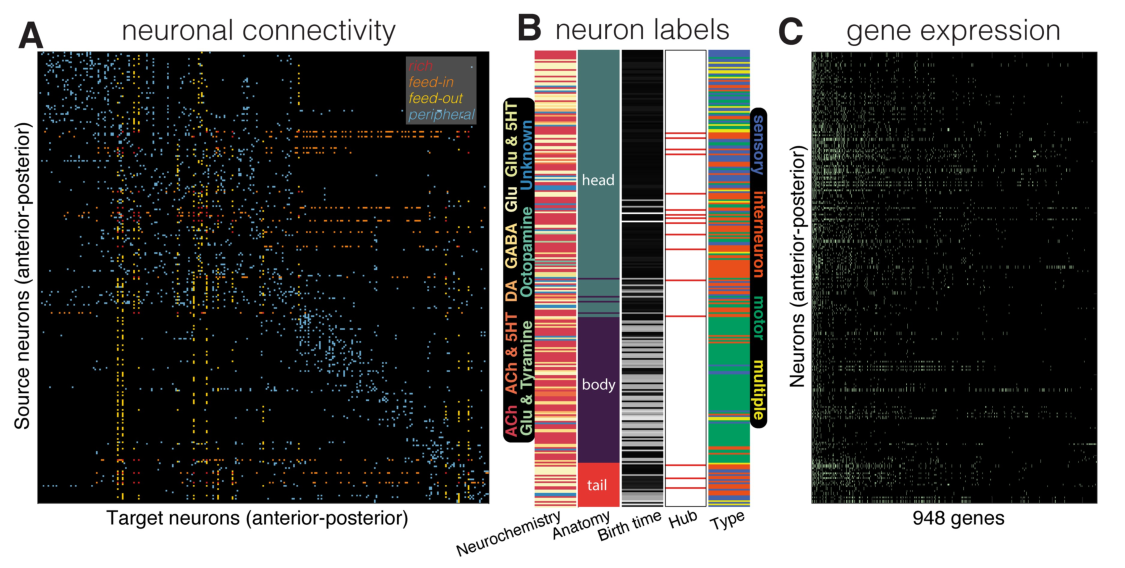
\includegraphics[width=1\textwidth]{Chapter2/Ch2Fig1.pdf}}
 \caption{\textbf{Schematic representation of the data used in this study.}
All plots show neurons (rows) ordered by anterior-posterior along the longitudinal axis, from the top of the head (upper, left) to the bottom of the tail (lower, right).
(A) Connectivity matrix summarized 2990 directed chemical and electrical connections between 279 neurons from neuron $i$ (row) to neuron $j$ (column).
Connections are colored according to how they connect hubs ($k > 44$) and nonhubs ($k \leq 44$), as `rich' (hub $\rightarrow$ hub), `feed-in' (nonhub $\rightarrow$ hub), `feed-out' (hub $\rightarrow$ nonhub), and `peripheral' (nonhub $\rightarrow$ nonhub).
(B) Neurochemistry (types as labeled), anatomical location (as labeled), birth time (from early born neurons, black, to late-born neurons, white), hub assignment (hubs labeled red), and functional type (as labeled).
(C) Binary gene expression indicated as a green dot when a gene (column) is expressed in a neuron (row).}
\label{fig:Ch2Fig1}
\end{figure}


\subsection*{Correlated gene expression}
Our primary aim in this work is to understand how pairwise patterns of neuronal connectivity (shown in Figure \ref{fig:Ch2Fig1}A) relate to coupled expression across 948 genes between pairs of neurons (i.e., pairs of rows of Figure \ref{fig:Ch2Fig1}C).
To estimate the coupling between neuronal gene expression profiles, we required a similarity measure for pairs of neurons that captures their similarity of gene expression profiles, or correlated gene expression (CGE).
We used a binary analogue of the linear Pearson correlation coefficient, the mean square contingency coefficient \citep{Warrens2008}:
\begin{equation} \label{eq:rphi}
    r_\phi = \frac{n_{11}n_{00} - n_{10}n_{01}}{\sqrt{n_{1\bullet}n_{0\bullet}n_{\bullet 0}n_{\bullet 1}}},
\end{equation}
for two vectors, $x$ and $y$, of length $L (=948)$, where $n_{xy}$ counts the number of observations of each of the four outcomes (e.g., $n_{10} = \sum_i \delta_{x_i,1}\delta_{y_i,0}$ counts the number of times $x=1$ and $y=0$), and the symbol $\bullet$ sums across a given variable (e.g., $n_{\bullet 0} = \sum_i \delta_{y_i,0}$ counts the number of times $y = 0$).
The coefficient assumes a maximum value $r_\phi = 1$ when $x$ and $y$ are identical (such that $n_{11} + n_{00} = L$), and a minimum value $r_\phi = -1$ when $x$ and $y$ are always mismatched (such that $n_{10} + n_{01} = L$).
Note that we use the notation $r_\phi$ to denote the phi coefficient, Eq.~\eqref{eq:rphi}; this notation should not be confused with the rich-club coefficient, $\phi(k)$.

One concern about applying this measure to sparsely annotated data is that it may be biased by differences in the number of expressed genes in a neuron, which ranged from 3 (0.3\% of 948 genes analyzed here) to 138 (14.6\%).
To explore this further, we compared $r_\phi$ with several other commonly used metrics of association between binary vectors including Yule's $Q$ and the Jaccard index.
While these other binary similarity metrics exhibited strong bias with the proportion of gene expression annotations made to a given neuron, $r_\phi$ was not biased (see Figure \ref{fig:Ch2S2_Fig} and \ref{app:AppendixCh2_2}).

The 92 bilateral pairs of neurons (e.g., AVAL/AVAR, CEPVL/CEPVR, etc.) exhibit highly correlated gene expression patterns: all bilateral pairs of neurons have $r_\phi > 0.8$, and 96\% of bilateral pairs have $r_\phi > 0.95$.
Although including bilateral pairs of neurons do not change the main results of this paper, to ensure that our results are not driven by the high CGE between bilateral pairs of neurons, we excluded CGE values of bilateral pairs of neurons from all analyses involving CGE.

\subsection*{Gene scoring and enrichment}
Our CGE measure, $r_\phi$, quantifies the similarity between the expression profiles of two neurons across all 948 genes.
To further investigate the role of individual genes in producing different CGE patterns, we developed a method for scoring the contribution of each individual gene to the overall correlation coefficient, following prior work using continuous gene expression data \citep{Fulcher2016}.
Performing similar analyses with \emph{C.elegans} data poses additional challenges due to:
(i) binary expression data, making robust quantification difficult;
(ii) sparse and incomplete data, posing statistical problems for quantifying a signal in genes with limited expression;
and (iii) low genome coverage (less than 5\% of the protein coding genes in \emph{C.elegans}), constraining our ability to perform a comprehensive enrichment analysis, e.g., using the Gene Ontology (GO) \citep{Ashburner2000}.

Given that $r_\phi$ treats mutual gene expression (i.e., cases in which a gene is expressed in pairs of neurons, $n_{11}$) the same as mutual absence of gene expression ($n_{00}$), we started by developing a new analytic measure of the probability of mutual gene expression, given its clearer biological interpretation (see \ref{app:AppendixCh2_3}).
This measure was not biased by differences in the relative number of expressed genes (Figure \ref{fig:Ch2S2_Fig}D) and yields qualitatively similar outputs to $r_\phi$ on our data.
Thus, while we use $r_\phi$ throughout this work for its ease of interpretation (as an analogue of the conventional correlation coefficient), our new probability-based CGE measure allowed us to motivate a method for quantifying the contribution of individual genes (and functional groups of genes) to patterns of CGE that addresses some of the above-mentioned challenges.
Note that our main findings, obtained using $r_\phi$, are replicated using our new CGE measure (Figure \ref{fig:Ch2S3_Fig}).

As a starting point, we quantified the contribution of individual genes to differences in CGE for different categories of neuron pairs, specifically for (i) increased CGE in connected compared to unconnected pairs of neurons, and (ii) increased CGE in rich and feeder compared to peripheral connections.
Note that our method scores genes on their contribution to differences in CGE between categories of pairwise connections.
We first scored each gene for whether it is more likely to be expressed in a given class of neuron pair over another as the probability of obtaining at least as many matches (defined as expression in both neurons of a pair) as observed under a random CGE null model using the binomial distribution:
\begin{eqnarray}
	\label{eq:CBinomialProbability}
     p^{(a)} = 1 - \sum_{i=0}^{m-1}\binom{n}{i} p_\mathrm{class}^{i}(1-p_\mathrm{class}^{n-i}),
\end{eqnarray}
where $m$ is the number of matches (a match indicates that a given gene was expressed in both neurons) on the class of neuron pairs of interest, $n$ is the total number of matches across all neuron pairs considered in the analysis, $p_\mathrm{class} = n_\mathrm{class}/M$ is the probability of the given class of inter-region pairs, as the total number of neuron pairs of that class, $n_\mathrm{class}$, divided by the maximum number of possible neuron pairs, $M$, for a given gene, indexed with $a$.
This score, $p^{(a)}$, can be interpreted as a $p$-value under the null hypothesis that the number of expression matches of gene $a$ is consistent with a purely random pattern of matches/mismatches across edges, giving lower values to genes with more matches in the edge class of interest (compared to an alternative set of edges) than expected by chance.
For reasons described earlier, bilateral pairs of neurons were excluded from all scoring procedures and, to ensure that each gene contributes a meaningful score, we imposed a data quality threshold on the number of possible matches, $n \geq 10$.

Our first analysis compares two mutually exclusive types of neuron pairs:
(i) all pairs of neurons that are connected by at least one chemical or electrical synapse, and
(ii) all pairs of neurons that are unconnected.
For this analysis, $p_\mathrm{class} = 0.059$ is the proportion of neuron pairs that are connected, $n$ is the total number of neuron pairs that both exhibit expression of gene $a$, and $m$ is the number of neuron pairs that are structurally connected for which both neurons express gene $a$.
A total of 414 (/948) genes had $n \geq 10$ for this analysis.
Our second analysis compares pairs of connected neurons for which at least one is a hub (i.e., rich, feed-in, or feed-out connections), to pairs in which both neurons are nonhubs (i.e., peripheral connections).
In this case, $p_\mathrm{class} = 0.35$ is the proportion of connected pairs of neurons that involve hubs, $n$ is the number of connected neuron pairs for which gene $a$ is expressed in both, and $m$ counts the number of connected neuron pairs involving hubs for which gene $a$ is expressed.
A total of 168 (/948) genes had $n \geq 10$ for this analysis.

As well as interpreting the list of individual genes that were significant after correcting for multiple hypothesis comparison, we performed an over-representation analysis (ORA) using the genes that contribute most to a given connectivity pattern to assess whether any gene sets (GO categories) were statistically over-represented in this list.
To obtain the gene list, we used the false discovery rate correction of Benjamini and Hochberg \citep{Benjamini1995} on $p$-values computed using Eq.~\eqref{eq:CBinomialProbability}, which were thresholded at a stringent level of $p = 10^{-4}$ (corresponding to approximately the top 20\% of genes in each analysis).
Over-representation for each biological process GO category with 5 to 100 genes available was quantified as an FDR-corrected $p$-value (across around 700 GO categories) using version 3.0.2 of \emph{ErmineJ} software \citep{Gillis2010}.
Biological process GO annotations \citep{Ashburner2000} were obtained from GEMMA \citep{Zoubarev2012} (using \texttt{Generic\_worm\_noParents.an.txt.gz} downloaded on March 31, 2017).
Gene Ontology terms and definitions were obtained in RDF XML file format downloaded from \url{archive.geneontology.org/latest-termdb/go_daily-termdb.rdf-xml.gz} on March $31$ $2017$.

\section{Results}

A schematic overview of our data is in Figure \ref{fig:Ch2Fig1}, including
the directed binary connectome (Figure \ref{fig:Ch2Fig1}A),
additional anatomical data gathered for each neuron (Figure \ref{fig:Ch2Fig1}B),
and binary gene expression across 948 genes (Figure \ref{fig:Ch2Fig1}C).
Our analysis is presented in five parts:
(i) given past evidence for a major effect of physical distance on connection probability and CGE  \citep{Fulcher2016}, we first characterize the spatial dependency of connection probability and CGE;
(ii) we confirm the rich-club organization of the \emph{C.elegans} connectome;
(iii) we show that CGE is increased in connected pairs of neurons relative to unconnected pairs, in electrical synapses relative to chemical synapses, and in connected hub neurons relative to other types of connected neuron pairs [mirroring previous results in the mesoscale mouse connectome \citep{Fulcher2016}];
(iv) we demonstrate that high CGE between connected hub neurons is not driven by factors like stereotypical interneuron expression, birth time, lineage similarity, neuromodulator types or expression similarity within modules, but may be driven by the high CGE of command interneurons;
(v) we characterize the contribution of specific genes, and broader gene ontology categories, to the observed patterns.

\subsection{Spatial dependency}
Previous work has demonstrated the importance of spatial effects in driving patterns of gene expression, with more proximal brain areas
\citep{Horvat2016,Wang2016,Markov2013,Henderson2014,Fulcher2016,Noori2017,Levy2012,Azulay2016} having both a increased connection probability and more similar gene expression profiles \citep{Krienen2016, Fulcher2016, Pantazatos2017, Richiardi2017} than more distance brain areas.
Unlike network analyses of mammalian brains, where all neurons are confined to a spatially contiguous organ, neurons of the \emph{C.elegans} nervous system are distributed throughout the entire organism, forming a dense cluster of 147 neurons in the head (all within 130\,$\mu$m), 105 sparser neurons in the body (spanning 1.02\,mm), which are predominantly motor neurons (75\%), and another dense cluster of 27 neurons in the tail (all within 90\,$\mu$m of each other), as plotted in Figure \ref{fig:Ch2Fig2}.
In order to examine the relationship between connectivity and CGE, we need to understand the spatial dependence of both connectivity and CGE to characterize the extent to which previously reported spatial dependencies of these measurements apply to the microscale nervous system of \emph{C.elegans}.

\begin{figure}[h]
\centering{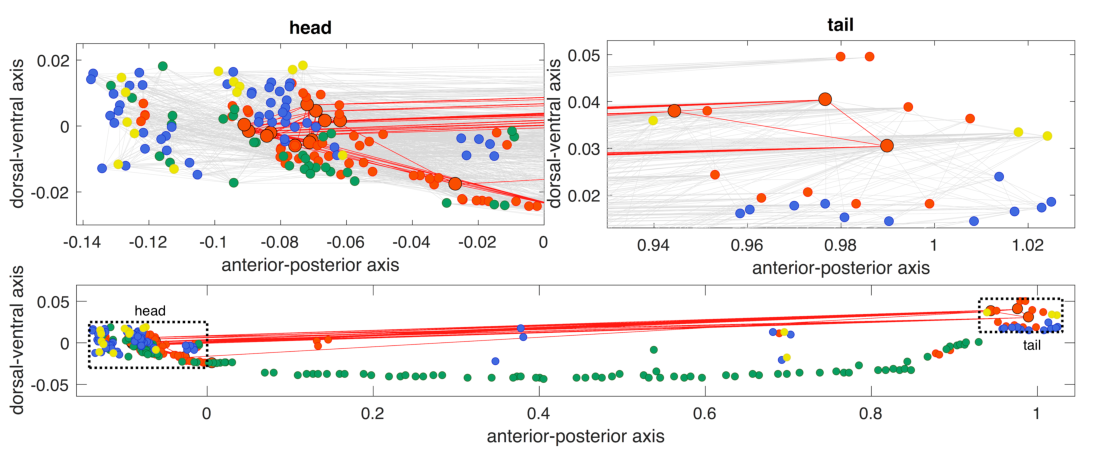
\includegraphics[width=1\textwidth]{Chapter2/Ch2Fig2.pdf}}
\caption{\textbf{Hub neurons are contained within the head and tail of \emph{C.elegans}}.
Neurons are positioned along the anterior--posterior (horizontal), and dorsal--ventral (vertical) axes, and are colored by type:
(i) interneuron (85 neurons, orange),
(ii) sensory (68 neurons, blue),
(iii) motor (108 neurons, green), or
(iv) multiple assignments (18 neurons, yellow).
Hub neurons (i.e., neurons with $k > 44$, see Figure \ref{fig:Ch2Fig5}) are shown as larger circles and outlined in black.
`Rich-club' connections between hub neurons are shown (red), and all other connections are also shown in the upper plots (gray).
Axes of each subplot are to scale with each other, and the upper zoomed-in plots of the head and tail are shown as dotted rectangles in the lower plot.}
\label{fig:Ch2Fig2}
\end{figure}

We first characterize the probability that two neurons will be connected given their source and target types, labeling each neuron as being in either the `head', `body', or `tail' of \emph{C.elegans}.
Connection probability is plotted as a function of Euclidean separation distance in Figure \ref{fig:Ch2Fig3} for each combination of source and target neuron labels, across 10 equiprobable distance bins (with exponential fits added for visualization).
Distinguishing connections by source and target neuron types uncovers clear spatial relationships (that are obscured when all connections are grouped, as in \citep{Azulay2016}), that differ across connection classes.
From the very short distance scale of $\lessapprox 100\,\mu$m of head$\rightarrow$head and tail$\rightarrow$tail connections to the very longest-range head$\rightarrow$tail and tail$\rightarrow$head connections ($\gtrapprox 1\,$mm), connection probability decreases with separation distance (Figure \ref{fig:Ch2Fig3}A).
For connections between pairs of neurons located in the body, ranging up to $\approx 1$\,mm, a near-exponential trend is exhibited, mirroring results in other species and across longer length scales \citep{Wang2016}, including mouse \citep{Goulas2017, Fulcher2016}, and in rodents and primates \citep{Horvat2016}.
Other connections do not exhibit strong spatial connectivity relationships, i.e., connections between the body and head or between the body and tail, shown in Figure \ref{fig:Ch2Fig3}B.

\begin{figure}[h]
  \centering{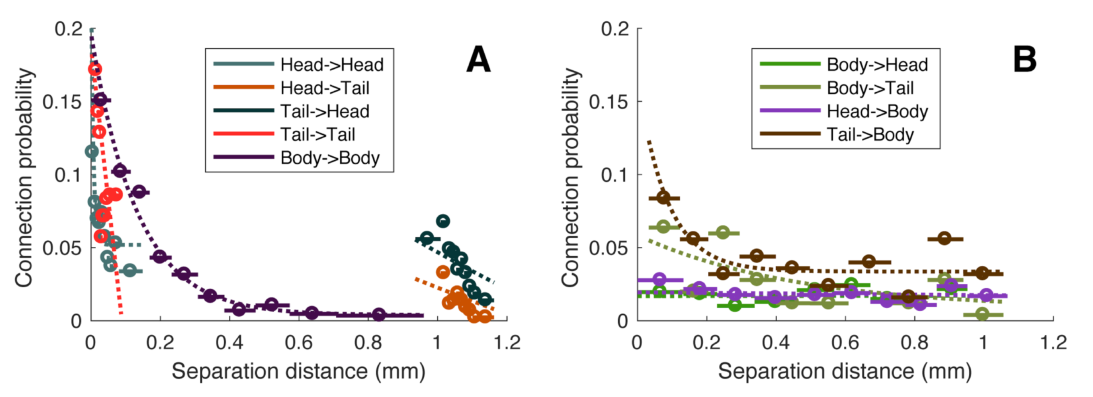
\includegraphics[width=1\textwidth]{Chapter2/Ch2Fig3.pdf}}
  \caption{
\textbf{Connection probability decreases with separation distance within and between the head and tail, and within the body.}
The connection probability for a pair of neurons as a function of their Euclidean distance is estimated in 10 equiprobable distance bins, shown as a circle (bin centers) and a horizontal line (bin extent).
There is a decreasing relationship for connections: within the head (aqua), from head$\rightarrow$tail (brown) and from tail$\rightarrow$head (stone blue), within the tail (red), and within the body (dark purple).
Exponential fits of the form $f(x) = A\exp(-\lambda x) + B$, some of which appear approximately linear across the range of the data, are shown as dotted lines.
(B)
Plots as in (A), but for connection classes between the body and head/tail: from body$\rightarrow$head (forest green), from body$\rightarrow$tail (dirt green), connections from head $\rightarrow$ body (purple), and from tail$\rightarrow$body (dark brown).
Apart from a small effect at short range for tail$\rightarrow$body connections, these connection classes show minimal distance dependence.}
\label{fig:Ch2Fig3}
\end{figure}

We next investigate the dependence of CGE, $r_\phi$, on the separation distance between neuron pairs, shown in Figure \ref{fig:Ch2Fig4}.
CGE decreases slightly with separation distance for the spatially close neurons within the head (Figure \ref{fig:Ch2Fig4}A) and within the tail (Figure \ref{fig:Ch2Fig4}B), but not for pairs of neurons involving the body (Figure \ref{fig:Ch2Fig4}C).
The decreasing trend in CGE with distance within the head and tail is primarily driven by a subset of nearby neurons with high $r_\phi$.
It may therefore represent a relationship specific to particular functionally related neurons, rather than a general, bulk spatial relationship seen in macroscopic mammalian brains \citep{Fulcher2016}.
Accordingly, attempting to correct for a bulk, non-specific trend by taking residuals from an exponential fitted to the relationship produced artifactual reductions in the CGE of many neuron pairs (shown in Figure \ref{fig:Ch2S4_Fig}).
Thus, we found no evidence for bulk spatial relationships of $r_\phi$ in the neuronal connectome of \emph{C.elegans}.

\begin{figure}[h]
  \centering{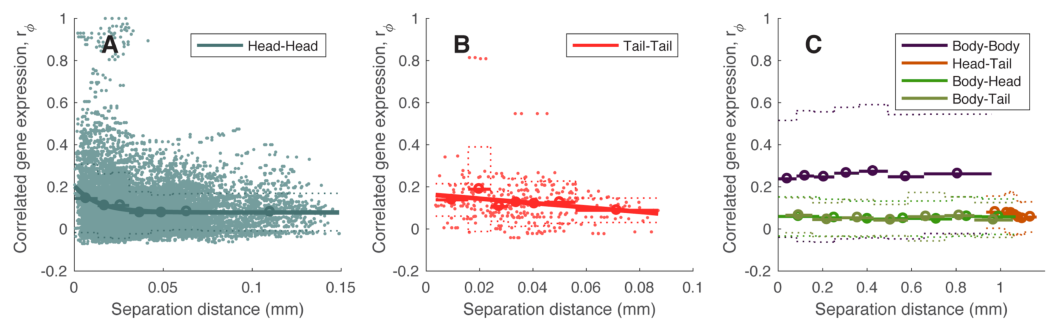
\includegraphics[width=1\textwidth]{Chapter2/Ch2Fig4.pdf}}
  \caption{
  \textbf{Dependence of correlated gene expression, $r_\phi$, on spatial separation between pairs of neurons.}
  Correlated gene expression, $r_\phi$ (excluding bilateral homologous pairs of neurons), is shown as a function of the pairwise separation distance between pairs of neurons (shown as the mean (solid) $\pm$ standard deviation (dotted) in seven equiprobable distance bins, with extent shown as horizontal bars), for (A) all pairs of neurons in the head, (B) all pairs of neurons in the tail, and (C) all other pairs (labeled).
  Scatters for all neuron pairs are added in (A) and (B).
  An exponential relationship, $f(x) = A\exp(-\lambda x) + B$, is fitted in (A) and (B).
  The weak decreasing trend in $r_\phi$ with distance, is primarily driven by a small subset of nearby neurons with high $r_\phi$, and may therefore represent a more specific relationship between particular neurons, rather than a general, bulk spatial relationship observed in macroscopic mammalian brains \citep{Fulcher2016, Krienen2016}.}
\label{fig:Ch2Fig4}
\end{figure}

\subsection{Hub connectivity}

Next we analyze the topological properties of the \emph{C.elegans} connectome, represented as a directed, binary connectivity matrix between 279 neurons, combining directed chemical synapses and undirected electrical gap junctions (Figure \ref{fig:Ch2Fig1}).
The degree distribution is shown in Figure \ref{fig:Ch2Fig5}A, where neurons are labeled as sensory neurons, interneurons, motor neurons, or neurons with multiple functional assignments.
Consistent with the results of \citet{Towlson2013},  who used an undirected version of the connectome (by ignoring the directionality of chemical synapses), we found a positively-skewed degree distribution containing an extended tail of high-degree hub interneurons.
Hub interneurons of \emph{C.elegans} are mostly command interneurons and mediate behaviors like coordinated locomotion and foraging \citep{Tsalik2003}.


\begin{figure}[!h]
   \centering{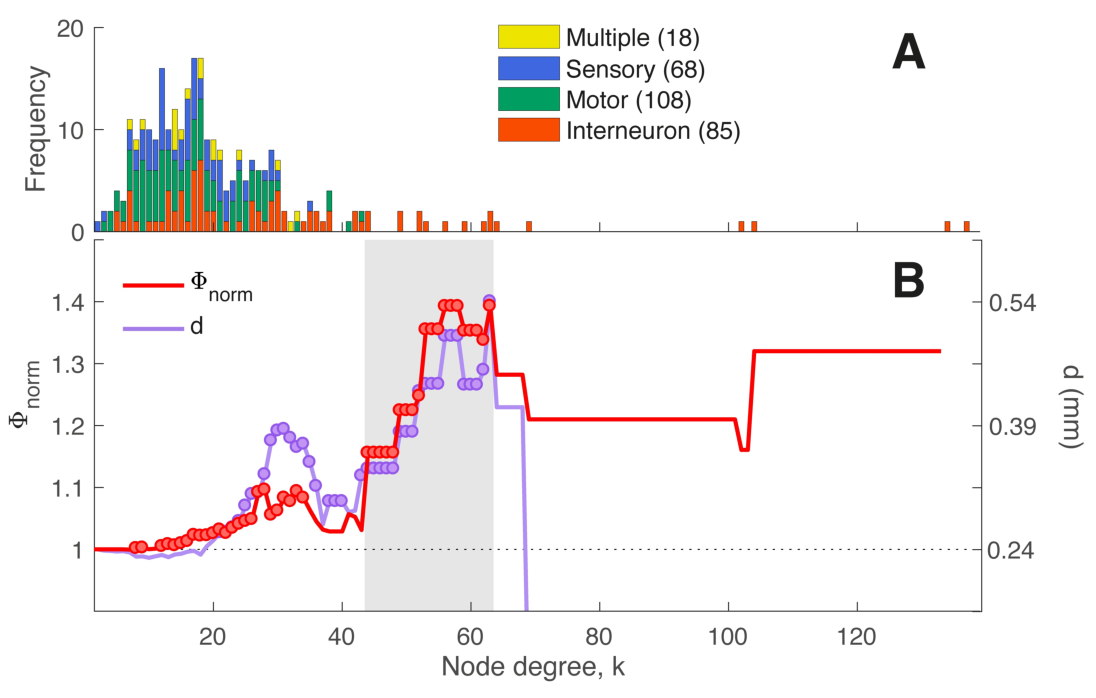
\includegraphics[width=1\textwidth]{Chapter2/Ch2Fig5.pdf}}
 \caption{\textbf{Rich-club organization of the \emph{C.elegans} connectome}.
(A) Degree distribution of neurons, labeled to four categories:
(i) interneuron (85 neurons, orange),
(ii) motor (108 neurons, green),
(iii) sensory (68 neurons, blue), or
(iv) multiple assignments (18 neurons, yellow).
The distribution features an extended tail of high-degree interneurons.
(B)
Normalized rich club coefficient, $\Phi_\mathrm{norm}$ (red), as a function of the degree, $k$, at which hubs are defined (as neurons with degree $>k$).
Also shown is the mean Euclidean separation distance, $d$ (purple) between connected hub regions (across degree thresholds, $k$).
$\Phi_\mathrm{norm} > 1$ indicates that hubs are more densely interconnected among each other than expected by chance, with red circles indicating values of $\Phi_\mathrm{norm}$ that are significantly higher than an ensemble of 1000 degree-matched null networks ($p < 0.05$).
Purple circles indicate where the Euclidean distance between connected pairs of hubs is significantly greater than the Euclidean distance for all other pairs of connected regions (right-tailed Welch's $t$-test, $p < 0.05$).
}
 \label{fig:Ch2Fig5}
\end{figure}

Using the normalized rich-club coefficient, $\Phi_\mathrm{norm}$, to quantify the extent to which hubs are densely interconnected, we confirmed the results of  
\citet{Towlson2013}, finding rich-club organization in the connectome, as shown in Figure \ref{fig:Ch2Fig5}B.
The figure plots the variation of $\Phi_\mathrm{norm}$ across degree thresholds, $k$, at which hubs are defined (as neurons with degree $>k$), with red circles indicating a significant increase in link density among hubs relative to 1000 degree-preserving nulls (permutation test, $p < 0.05$).
The plot reveals rich-club organization ($\Phi_\mathrm{norm} > 1$) at the upper tail of the degree distribution, particularly across the range $44 < k < 63$, shaded gray in Figure \ref{fig:Ch2Fig5}B.
Similar results were obtained using weighted representations of the connectome (i.e., using information about the number of synapses in the connectivity network) for two different definitions of the weighted rich-club coefficient \citep{Opsahl2008}, shown in Figure \ref{fig:Ch2S5_Fig}.
Throughout this work, we define a set of hubs as the sixteen neurons with $k > 44$, which corresponds to the lowest degree threshold at which the network displays a contiguous region of significant rich-club organization at high $k$.
Our list of hubs includes all of the 11 hub neurons of \citet{Towlson2013} at $3 \sigma$ (see Figure \ref{tab:HubList}), with five additional hubs identified in our analysis of the directed connectome.

The rich-club connectivity of the \emph{C.elegans} connectome is accompanied by an increase in mean hub-hub connection distance \citep{Towlson2013}, with a significant increase through the topological rich-club regime (right-tailed Welch's $t$-test, $p < 0.05$), shown in Figure \ref{fig:Ch2Fig5}B.
This can be attributed to a relative increase in long-distance hub-hub connections between the head and tail, shown in Figure \ref{fig:Ch2Fig2} (Figure  \ref{fig:Ch2S6_Fig}).
The high connection density and long mean anatomical distance between pairs of hub neurons counters the general trend in the \emph{C.elegans} connectome, where the probability of connectivity between two neurons decays with their separation distance (Figure \ref{fig:Ch2Fig3}).
These results are consistent with previous findings across diverse neural systems and suggest that the rich club may provide a central yet costly backbone for neuronal communication in \emph{C.elegans} \citep{VandenHeuvel2012, Towlson2013}.

\subsection{Correlated gene expression and connectivity}

We next investigate how the network connectivity properties of \emph{C.elegans} relate to patterns of CGE, using the mean square contingency coefficient, $r_\phi$.
To test whether CGE varies as a function of connectivity, we compared the distribution of $r_\phi$ between
(i) all connected pairs of neurons, and
(ii) all unconnected pairs of neurons.
Connected pairs of neurons have more similar expression profiles than unconnected pairs (Wilcoxon rank-sum test, $p = 1.8 \times 10^{-78}$).
Figure~\ref{fig:Ch2Fig6}A (left) shows distributions of $r_\phi$ for:
(i) all pairs of neurons that are connected via electrical gap junctions (474 pairs, after excluding bilateral pairs),
(ii) all pairs of neurons that are connected via reciprocal (291 pairs) and,
(iii) unidirectional chemical synapses (1721 pairs) as well as
(iv) all pairs of neurons that have neither connection (\num{36450} pairs).
Note that 175 pairs of neurons are connected by both chemical synapses and gap junctions, and are thus included in both chemical and electrical categories.
Amongst connected pairs of neurons, those connected via gap junctions exhibit more similar gene expression profiles than those connected via chemical synapses (Wilcoxon rank-sum test, $p = 5.4 \times 10^{-22}$).
We found no difference in CGE between pairs of neurons connected reciprocally by chemical synapses ($N_1 \leftrightarrow N_2$ for two neurons $N_1$ and $N_2$) versus those connected unidirectionally ($N_1 \rightarrow N_2$) (Wilcoxon rank-sum test, $p = 0.99$).

We next investigated whether CGE varies across different types of connections defined in terms of their hub connectivity.
For a given hub threshold, $k$, we first labeled each neuron as either a `hub' (nodes with degree $> k$) or a `nonhub' (degree $\leq k$), and then labeled each connection as either `rich' (hub $\rightarrow$ hub), `feed-in' (nonhub $\rightarrow$ hub), `feed-out' (hub $\rightarrow$ nonhub), or `peripheral' (nonhub $\rightarrow$ nonhub).
The median CGE, $\tilde{r}_\phi$, of each of these four connection types is plotted in Figure \ref{fig:Ch2Fig6}B, with circles indicating statistically significant increases of a given connection type relative to all other connections (one-sided Wilcoxon rank-sum test, $p < 0.05$).
Correlated gene expression in rich connections increases with degree, $k$, particularly in the topological rich-club regime where hubs are densely interconnected (shaded gray in Figure \ref{fig:Ch2Fig6}B).
In this topological rich-club regime, both feed-in and feed-out connections exhibit increased CGE relative to peripheral connections, which show the lowest levels of CGE.
Full distributions of $r_\phi$ for each edge type at a hub threshold of $k > 44$ are in Figure \ref{fig:Ch2Fig6}A (right).
This plot shows that, compared to all different types of pairs of neurons, connected pairs of hubs showed the highest CGE.

In summary, our results reveal:
(i) increased CGE in connected pairs of neurons;
(ii) the highest CGE in rich connections; and
(iii) lowest CGE in peripheral connections.
These results, obtained using incomplete binary annotations of gene expression across 948 genes in a microscale neuronal connectome, are consistent with a prior analysis of the expression of over \num{17000} genes across 213 regions of the mesoscale mouse connectome \citep{Fulcher2016}.

\subsection{Potential drivers of elevated correlated gene expression between hubs}
The sixteen hub neurons in \emph{C.elegans} ($k > 44$):
are all interneurons,
are all located in either the head or tail,
are mostly contained within a single topological module of the network,
are mostly cholinergic (13/16),
and are all born prior to hatching.
We therefore investigated whether the similarity of gene expression profiles between hubs is specific to their high levels of connectivity, or whether it could instead be driven by these other characteristics.

\begin{figure}[!h]
 \centering{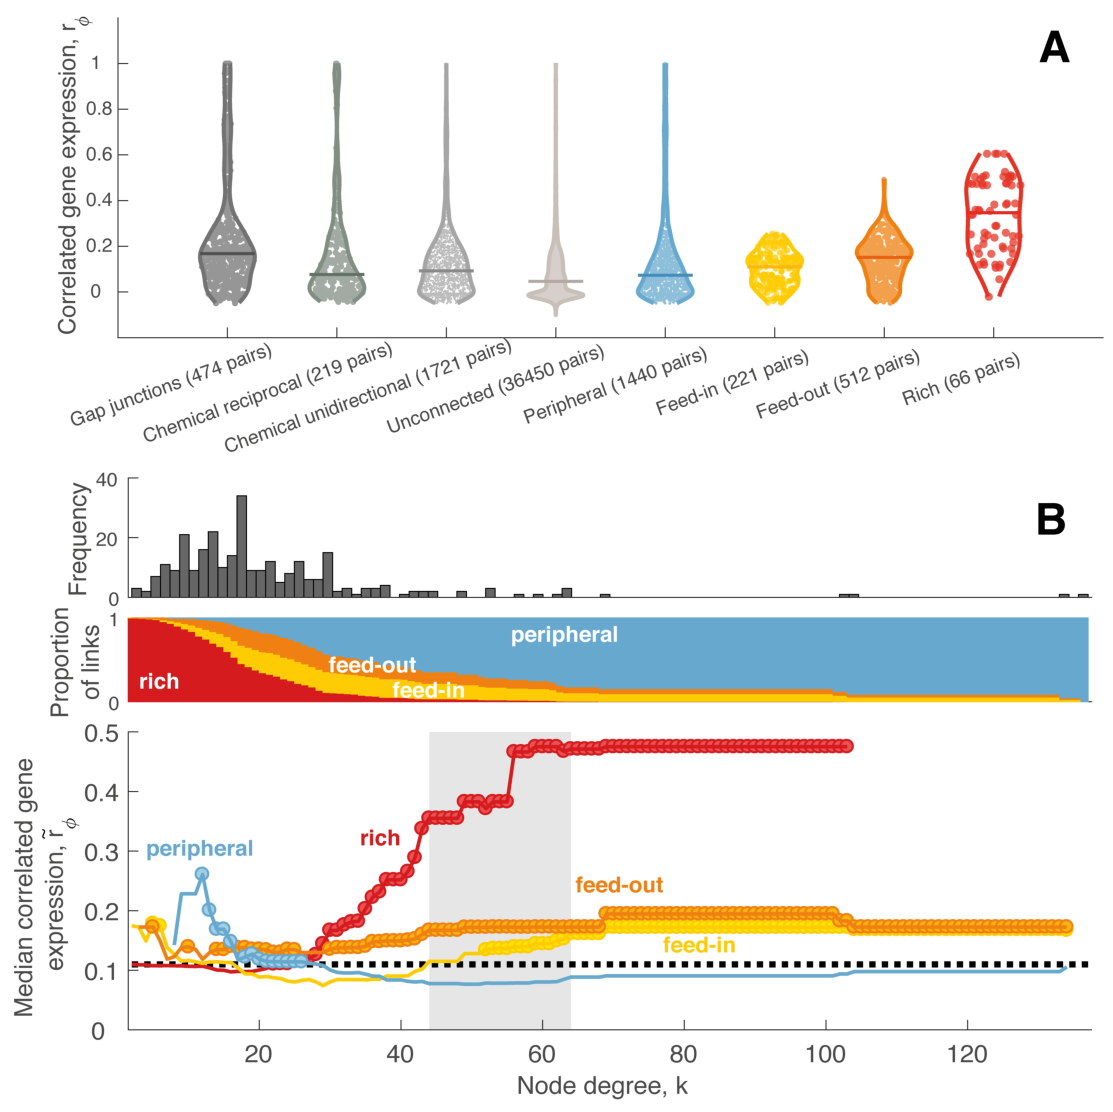
\includegraphics[width=0.85\textwidth]{Chapter2/Ch2Fig6.pdf}}
\caption{{\bf Correlated gene expression varies as a function of connectedness and connection type.}
(A) \textit{Left}: distribution of CGE for (i) pairs of neurons connected by gap junctions, (ii) pairs of neurons connected by reciprocal chemical synapses, (iii) pairs of neurons connected by unidirectional chemical synapses, (iv) pairs of neurons that are unconnected, shown as a violin plot, with the median of each distribution represented by a horizontal line.
CGE is increased in connected (electrical or chemical; reciprocally or unidirectionally) pairs of neurons relative to unconnected pairs ($p = 1.8 \times 10^{-78}$, Wilcoxon rank sum test).
Among connected pairs of neurons neurons connected via gap junctions have more similar CGE than connected via chemical synapses (Wilcoxon rank-sum test, $p = 5.4 \times 10^{-22}$).
\textit{Right}: GCE for pairs of neurons labeled as peripheral, feed-in, feed-out, and rich, where hubs are neurons with degree $k>44$. The median of each distribution shown as a horizontal line.
CGE is significantly higher between hubs (rich links) compared to feeder ($p = 5 \times 10^{-22}$, Wilcoxon rank sum test) and peripheral ($p = 3.9 \times 10^{-19}$, Wilcoxon rank sum test) links.
Feed-out links show significantly higher CGE than both feed-in ($p = 1.9 \times 10^{-6}$, Wilcoxon rank sum test) and peripheral links ($p = 4.5 \times 10^{-12}$, Wilcoxon rank sum test).
(B)
\emph{Top}: Degree distribution, $k$, of the \emph{C.elegans} connectome.
\emph{Middle}: proportion of connections that are:
`rich' (hub$\rightarrow$hub, red),
`feed-in' (nonhub$\rightarrow$hub, yellow),
`feed-out' (hub$\rightarrow$nonhub, orange), or
`peripheral' (nonhub$\rightarrow$nonhub, blue) as a function of the degree threshold, $k$, used to define hubs.
Note that at high $k$ most neurons are labeled as nonhubs and hence the vast majority of connections are labeled `peripheral'.
 \emph{Bottom}: Median CGE, $\tilde{r}_\phi$, for each connection type as a function of $k$.
The median CGE across all network links is shown as a dotted black line; the topological rich-club regime (determined from the network topology, Figure \ref{fig:Ch2Fig5}) is shaded gray.
Circles indicate a statistically significant increase in CGE in a given link type relative to the rest of the network (one-sided Wilcoxon rank-sum test, $p < 0.05$).
}
 \label{fig:Ch2Fig6}
\end{figure}

\paragraph{Interneurons.}
The sixteen hubs in \textit{C.elegans} are all interneurons.
To determine whether the increase in CGE in rich connections was specific to interneurons, we plotted the median CGE for hub-hub connections, $\tilde{r}_\phi$, as a function of the degree threshold, $k$, separately for connections involving interneurons, sensory neurons, and motor neurons, as shown in Figure \ref{fig:Ch2Fig7}B.
For the curve labeled `sensory', for example, each point is the median $\tilde{r}_\phi$ across connections involving sensory neurons (i.e., at least one neuron of a connected pair is a sensory neuron), for which both neurons have degree $>k$.
The increase in median hub-hub CGE is strongest for connections involving interneurons.
Motor neurons show a smaller increase with $k$, although the absence of motor and sensory neurons with high {$k$ makes it difficult to draw firm conclusions.
However, we do find that CGE is higher for hub-hub pairs of interneurons compared to connections between all pairs of nonhub interneurons (Wilcoxon rank sum test, $p = 5 \times 10^{-21}$), indicating that the high CGE of rich pairs cannot simply be related to the fact that all hub neurons are interneurons (Figure \ref{fig:Ch2Fig7}C).
We next investigated whether greater CGE of hub-hub pairs of neurons could be driven by specific anatomical properties of hub interneurons.
Specifically, we selected a subset of nonhub interneurons that most closely resemble the anatomical properties of hub interneurons in terms of their position and projection pattern; that is, the cells are in similar locations in the head and their axons project to similar targets in the tail. These neurons were AVFL, AVFR, AVHL, AVHR, AVKR, AVJL, and AVJR.
Pairs of hub interneurons show higher median CGE than pairs of anatomically-matched nonhub interneurons, with the difference being at the threshold of statistical significance (Wilcoxon rank sum test, $p = 0.051$), suggesting that the increase in CGE amongst hub interneurons is not a consequence of them being interneurons.

\begin{figure}[!h]
\centering{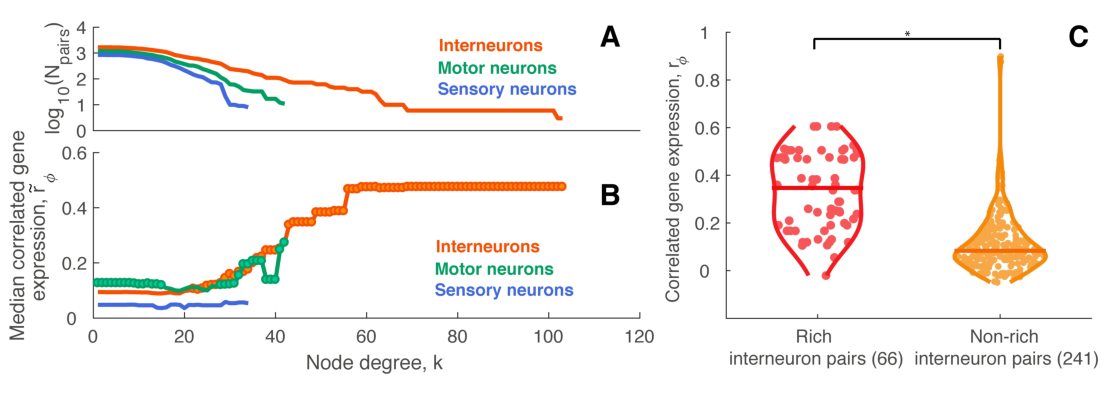
\includegraphics[width=1\textwidth]{Chapter2/Ch2Fig7.pdf}}
 \caption{
\textbf{Correlated gene expression is highest for hub interneurons.}
(A) The number of connected neuron pairs involving interneurons (orange), sensory neurons (blue), and motor neurons (green) across degree threshold, $k$, represented as $\log_{10}$(number of links).
(B) Median CGE as a function of degree for connections involving different types of neurons.
Circles indicate a statistically significant increase in CGE in a given link type relative to the rest of the network (one-sided Wilcoxon rank-sum test, $p < 0.05$).
(C) CGE distributions for connected pairs of hub interneurons (red) and connected pairs of non-hub interneurons (dark yellow) (Wilcoxon rank sum test, $p = 5 \times 10^{-21}$). * represents statistically significant difference.
}
 \label{fig:Ch2Fig7}
\end{figure}

\paragraph{Modular organization.}

Prior work in humans has shown that functional networks in the brain have elevated transcriptional coupling \citep{Richiardi2015}.
The \emph{C.elegans} connectome has a modular organization, with prior work decomposing it into:
(i) modules of neurons with dense intra-module connectivity (and relatively sparse connectivity between modules) \citep{Kim2014a, Pan2010, Bassett2010}, or
(ii) groups of neurons with more similar connectivity patterns within groups than between groups \citep{Achacoso1992, Pavlovic2014}.
We therefore examined the association between topological modularity of the \emph{C.elegans} connectome and CGE.
We used the Louvain community detection algorithm \citep{Blondel2008} to extract modules from the \emph{C.elegans} connectome using consensus clustering (see \textit{Methods}).
Four modules were extracted, with eleven hubs in module one (which contains 111 neurons), four hubs in module two (96 neurons), one hub in module three (40 neurons), and no hubs in module four (32 neurons).
We also compared the results of this modular partition of neurons to a previously reported nine-module partition derived from an Erd\"os-R\'enyi Mixture Model (ERMM) \citep{Pavlovic2014}.
For the Louvain consensus modules, CGE, $r_\phi$, was significantly increased for connected neurons in the same module (1552 pairs) relative to connected pairs in different modules (687 pairs) (Wilcoxon rank sum test, $p = 6.6 \times 10^{-4}$), but there was no significant difference between intra-modular connected neurons and inter-modular connected neurons for the nine-module ERMM partition (Wilcoxon rank sum test, $p = 0.46$).
The resolution and type of modular decomposition thus affects the relationship between CGE, connectivity, and modular network structure in \emph{C.elegans}.

We then tested whether connected hubs exhibit more similar CGE within and between modules (for both the consensus Louvain and ERMM modular decompositions).
For pairs of connected neurons within the same module, $r_\phi$ is higher for pairs of hubs than pairs of nonhubs (Wilcoxon rank sum test, $p = 6.9\times 10^{-17}$ for consensus Louvain modules, shown in Figure \ref{fig:Ch2Fig8}A; $p = 9.3 \times 10^{-7}$ for ERMM partition).
We found a similar result for connected neurons in different modules: pairs of connected hubs exhibit increased CGE than other types of connected pairs of neurons (Wilcoxon rank sum test, $p = 1.6 \times 10^{-5}$ for consensus Louvain modules, shown in Figure \ref{fig:Ch2Fig8}B; $p = 1.6 \times 10^{-16}$ for ERMM).
Thus, for both types of modular decompositions considered, intra-modular and inter-modular connections involving hub neurons exhibit more correlated gene expression patterns than other intra-modular and inter-modular connections.

\paragraph{Lineage distance.}
The lineage distance between a pair of neurons is defined as the sum of total divisions that have taken place since the most recent common ancestor cell \citep{Pavlovic2014, Sulston1977, Sulston1983}.
In the mammalian brain, neuronal lineage has been associated with both functional properties \citep{Ciceri2013, Li2012} as well as connectivity \citep{Yu2012}.
Moreover, tissue distance (resembling lineage distance on a cellular scale) correlates with gene expression divergence, meaning that tissues from the same branch on the fate map share more similar gene expression patterns in both human and mouse mesoderm as well as ectoderm tissues \citep{Cui2007}.
Given that the ectoderm eventually differentiates to form the nervous system, this finding suggests a possible relationship between lineage distance and CGE in a microscale neuronal system such as that of \textit{C.elegans}.
However, we find no significant correlation between lineage distance and CGE in \textit{C.elegans} (Spearman's $\rho = -0.027$, $p = 0.2$).
As shown in Figure \ref{fig:Ch2Fig8}C, there was only a weak tendency for the meadian lineage distance to be increased in non-rich pairs (Wilcoxon rank sum test, $p = 0.079$).
Thus, we can not attribute the transcriptional similarity of connected hub neurons to their neuronal lineage.

\begin{figure}[H]
\centering{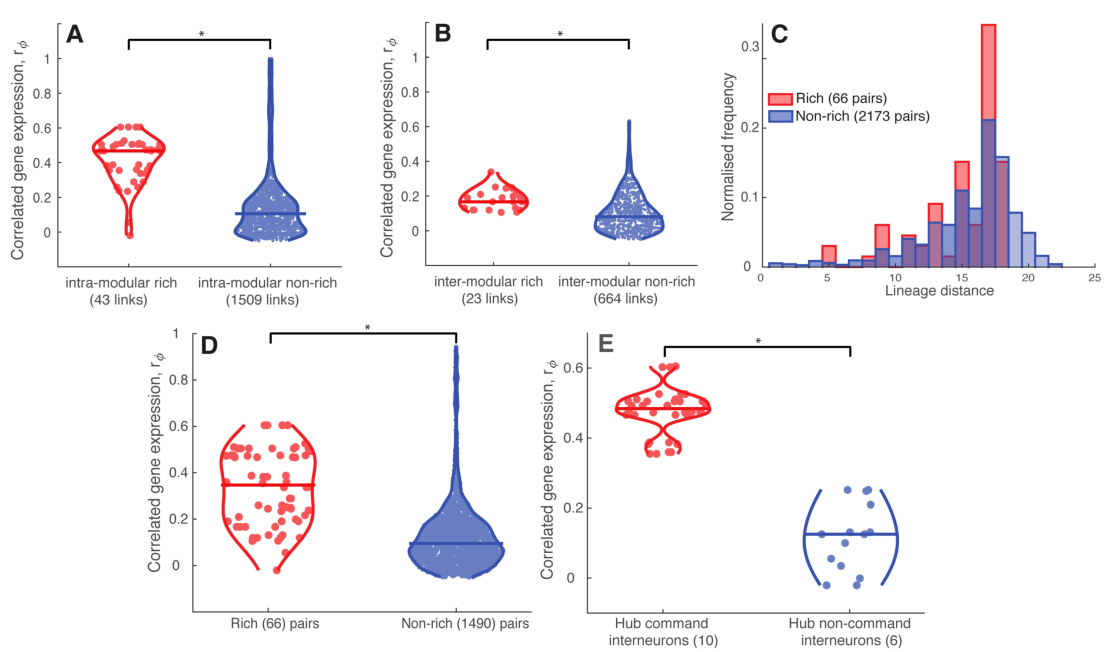
\includegraphics[width=1\textwidth]{Chapter2/Ch2Fig8.pdf}}
 \caption{
 \textbf{Increased CGE of hub neurons is not driven by modularity, neuronal birth time, or cell lineage distance.}
(A) Distributions of CGE, $r_\phi$, for intra-modular rich (red) non-rich (blue) connections, shown as violin plots with the median shown as a horizontal bar (Wilcoxon rank sum test, $p = 6.9 \times 10^{-17}$).
(B) Distributions of CGE, $r_\phi$, for inter-modular rich (red) and non-rich (blue) connections, shown as violin plots with the median shown as a horizontal bar (Wilcoxon rank sum test, $p = 1.6 \times 10^{-5}$).
(C) Distributions of lineage distance between rich links (red) and non-rich links (blue), plotted as histograms due to a discrete nature of this measure (Wilcoxon rank sum test, $p = 0.079$).
(D) Distributions of CGE, $r_\phi$, between early born hubs (rich links, red) and nonhubs (non-rich links, blue) shown as violin plots with the median shown as a horizontal bar (Wilcoxon rank sum test, $p = 3.9 \times 10^{-22}$).
(E) Distributions of CGE between hub command interneurons (red) and hub non-command interneurons (blue) shown as violin plots with the median shown as a horizontal bar (Wilcoxon rank sum test, $p = 3.3 \times 10^{-8}$).
* represents statistically significant differences.
}
 \label{fig:Ch2Fig8}
\end{figure}


\paragraph{Birth time.}
The genesis of neurons in \emph{C.elegans} is separated into two distinct time periods: before hatching (birth time $<550$ min -- `early-born') and after hatching (birth time $>1200$ min -- `late-born'), with no neurons formed during intermediate times \citep{Varier2011}.
As a broad group, connected pairs of early-born neurons do not exhibit significantly different CGE compared to connected pairs of late-born neurons (Wilcoxon rank sum test, $p = 0.64$), but connected pairs of early-born neurons do exhibit significantly higher CGE relative to pairs of connected neurons for which one neuron is born prior to hatching and the other is born after hatching (Wilcoxon rank sum test, $p = 4.2 \times 10^{-3}$).
Since all \emph{C.elegans} hub neurons are born prior to hatching \citep{Towlson2013} and neurons born at similar times may share similar connectivity properties \citep{Varier2011, Towlson2013}, we investigated whether the increase in CGE between hub neurons of \emph{C.elegans} may be driven by their similar birth times.
Focusing on the 201 neurons born prior to hatching (16 hub and 185 nonhub neurons), connected pairs of hub neurons exhibit significantly increased CGE, $r_\phi$, relative to other pairs of connected early-born neurons (Wilcoxon rank sum test, $p < 10^{-22}$), as shown in Figure \ref{fig:Ch2Fig8}D.

\paragraph{Neurochemistry.}
Hub neurons ($k > 44$) consist of thirteen cholinergic neurons, two glutamatergic neurons, and one neuron of unknown neurotransmitter type \citep{Pereira2015}.
We find that neuron pairs show different CGE relationships as a function of their neurotransmitter type, e.g., pairs of GABAergic neurons have high median CGE, $\tilde{r}_\phi = 0.59$, while pairs of glutamatergic neurons exhibit a relatively low median CGE, $\tilde{r}_\phi = 0.08$.
To determine whether the similarity in CGE between pairs of hub neurons is associated with their neurotransmitter types, we constructed $10^8$ random sets of sixteen neurons of the same neurotransmitter types as hubs (e.g., thirteen random cholinergic neurons, two random glutamatergic neurons, and one random neuron of an unknown neurotransmitter type) and compared the distribution of median CGE of each group to the median CGE of hub neurons as a permutation test.
Neurochemical identity is not associated with the elevated CGE of hub neurons, with hubs displaying a significant increase in median CGE relative to random sets of neurons with the same neurotransmitter types as hubs (permutation test, $p = 3\times10^{-4}$).

\paragraph{Anatomical location.}
Of the sixteen hub neurons, thirteen are in the head and three are in the tail; none are located in the body.
CGE varies as a function of anatomical location (i.e., `head', `body', and `tail'), with pairs of neurons in the same anatomical class exhibiting the highest median CGE (e.g., pairs of neurons within the body have a median $\tilde{r}_\phi = 0.14$, pairs of neurons within the tail have $\tilde{r}_\phi = 0.12$, and pairs of neurons within the head have $\tilde{r}_\phi = 0.07$), followed by lower median CGE in mixed classes (e.g., head-body pairs of neurons have $\tilde{r}_\phi = 0.01$).
Given this variation, we tested whether the increased CGE between hub neurons could be explained by their anatomical distribution using the permutation testing procedure described above for neurochemistry.
That is, we compared the distribution of CGE between hubs to a null distribution formed from $10^8$ random permutations of thirteen head neurons and three tail neurons.
The median CGE, $\tilde{r}_\phi$, between hub neurons is significantly increased relative to random sets of thirteen head neurons and three tail neurons (permutation test, $p = 8\times10^{-8}$).
Furthermore, CGE is significantly increased amongst hub neurons relative to other pairs of head neurons (Wilcoxon rank sum test, $p = 4.1 \times 10^{-11}$ for 46 hub-hub pairs and \num{1186} others),
and also amongst head/tail pairs of neurons (Wilcoxon rank sum test, $p = 1.6 \times 10^{-14}$ for 23 hub-hub pairs, 174 others),
but not for the three hub neurons in the tail (Wilcoxon rank sum test, $p = 0.15$ for three hub-hub pairs, 53 others).
Thus, anatomical location does not explain the high CGE of hub neurons.

\paragraph{Functional class.}
\emph{C.elegans} neurons can be divided into distinct groups that each perform a specialized behavioral function \citep{Hobert2003}.
One of the best-characterised functional classes that is particularly relevant for our analysis is the set of `command interneurons' -- a functional group of ten neurons that govern forward (AVBL, AVBR, PVCL, PVCR) and backward (AVAL, AVAR, AVDL, AVDR, AVEL, AVER) locomotion \citep{Rakowski2013}.
All of these neurons are hubs.
Given the overlap between hub neurons and command interneurons, we investigated whether command interneurons exhibit more similar expression than other hub interneurons, and may therefore drive the increase in CGE amongst hubs as a whole.
We compared CGE, $r_\phi$, between all pairs of command interneurons (ten neurons), and between all pairs of hubs that are not command interneurons (six neurons), shown in Figure \ref{fig:Ch2Fig8}E.
Correlated gene expression between command interneurons is significantly greater than between other hub neurons (Wilcoxon rank sum test, $p = 3.3 \times 10^{-8}$), indicating that command interneurons play a major role in driving the increased CGE amongst hub neurons.
Moreover, there is no difference in CGE between pairs of hubs that are not command interneurons (DVA, RIBL, RIBR, AIBR, RIGL, AVKL) and a set of seven anatomically matched nonhub head interneurons (AVFL, AVFR, AVHL, AVHR, AVJL, AVJR, AVKR) (Wilcoxon rank sum test, $p = 0.13$), indicating that the status of many hub neurons as command interneurons makes a significant contribution to the elevated CGE between hubs.

\subsection{Genes driving correlated gene expression patterns}

Having characterized a robust relationship between CGE and (i) connectivity, and (ii) hub connectivity, we next investigated which specific genes contribute most to this relationship.
Despite challenges with the incomplete binary expression measurements in a small proportion of the genome, we developed a method to score genes according to their contribution to a given CGE pattern (see \ref{Ch2Methods}).
We characterized individual high-scoring genes, with $p_\mathrm{corr} < 10^{-4}$ (approximately 20\% of genes with the highest scores in each analysis), and attempted to summarize functional groups of genes as biological process categories of the gene ontology (GO) that were enriched in high scoring genes using overrepresentation analysis (ORA) \citep{Ashburner2000, Gillis2010}.

We first investigated which genes drive increased CGE in connected pairs of neurons relative to unconnected pairs.
Previous studies in mouse have indicated that genes driving an increase in CGE between connected pairs of brain regions are enriched in GO categories related to neuronal connectivity and communication \citep{Fulcher2016, Ji2014, Fakhry2015a, French2011}.
First, we manually investigated individual high-scoring genes [i.e., those with $p_\mathrm{corr} < 10^{-4}$, see Supplementary Data File (\ref{file:geneList})].
Given that glutamate is a prevalent neurotransmitter in \textit{C.elegans} [26\% of neurons with known neurotransmitter type are glutamatergic \citep{Pereira2015}], it is appropriate that many high scoring genes are related to glutamate receptors (including \emph{glr-1}, \emph{glr-2}, \emph{glr-4}, \emph{glr-5}, \emph{nmr-1}, and \emph{nmr-2}).
Consistent with the importance of innexins in forming electrical synapses \citep{Starich2001}, our list contained the following innexin genes: \emph{unc-9}, \emph{unc-7}, \emph{inx-7}, \emph{inx-19}, \emph{inx-13}.
Genes encoding cell adhesion molecules related to axon outgrowth and guidance, cell migration and locomotion (\emph{sax-3}, \emph{cam-1}, \emph{unc-6}, \emph{rig-1}, \emph{unc-5}), learning (\emph{casy-1}) \citep{Zallen1999, Garriga1999, Leung-Hagesteijn1992, Harris2010, Ikeda2008},
as well as genes involved in determining cell polarity (\emph{vang-1}, \emph{prkl-1}) \citep{Wu2006, Hoffmann2010} were also amongst the top scoring genes for connectivity.
These genes have been implicated in neuronal connectivity in both flies and humans \citep{Paemka2013, Ehaideb2016, Sowers2013}, with our results predicting that they may play a similar role in \textit{C.elegans}.
In addition, transcription factors regulating neuronal development,
fate specification (\emph{lin-11}, \emph{unc-3}, \emph{unc-42}, \emph{ceh-14}, \emph{ast-1}, \emph{cfi-1}) \citep{Sarafi-Reinach2001, Prasad2008, Baran1999, Cassata2000, Schmid2006, Shaham2002a},
and locomotion (\emph{unc-3}) \citep{Prasad2008} were also implicated in driving increased CGE amongst connected pairs of neurons.
Both adhesion molecules and transcription factors are candidates for facilitating signal transduction and communication.

In order to summarize the above mentioned results and determine if any particular functional groups of genes are dominating in driving this effect, we performed an enrichment analysis.
Top scoring biological process GO categories from ORA analysis (of 85 genes relative to the 414 genes with sufficient data for this analysis) are listed in \ref{tab:enrichmentCON}.
Although no GO categories are significant at a false discovery rate of 0.05, the top categories are consistent with a connectivity profile, including `glutamate receptor signaling', `cell surface receptor signaling', and `ion transport', with other categories involved in regulation of growth rate and several related to catabolic processes.
Thus, despite incomplete gene expression data that do not provide sufficient coverage to detect statistically significant effects, these results indicate that our data-driven gene scoring method is able to yield sensible, biologically relevant insights into the genetic basis of neuronal connectivity in \textit{C.elegans} connectome.

Having characterized genes that contribute to the increase in CGE between connected pairs of neurons, we next investigated whether particular functional groups of genes drive differences in CGE between connections involving hub neurons (i.e., in rich, feed-in, and feed-out connections) relative to connections between pairs of nonhub neurons (i.e., peripheral connections).
In order to investigate which specific genes contribute most to the increase in CGE for connections involving hubs, we first investigated the highest-scoring genes, with $p_\mathrm{corr} < 10^{-4}$ (corresponding to approximately the top 20\% of genes in the analysis).
In addition to glutamate receptor genes (\emph{glr-5}, \emph{nmr-1}, \emph{nmr-2}, \emph{glr-1}, \emph{glr-2}, \emph{grld-1})
and acetylcholine related genes (\emph{ace-2}, \emph{cho-1}, \emph{unc-17}, \emph{deg-3}),
we again find a high number of genes regulating cell adhesion (\emph{cam-1}, \emph{rig-1}, \emph{rig-6}, \emph{unc-6}, \emph{grld-1}, \emph{dbl-1}, \emph{ncam-1})
and relevant transcription factors (\emph{unc-3}, \emph{unc-42}, \emph{ast-1}).
The implication of glutamate and acetylcholine may be attributable to the importance of glutamate in the regulation of locomotion in command interneurons \citep{Choi2015, Zheng1999}, with acetylcholine being the dominant neurotransmitter in hubs (13 out of 16 hubs are cholinergic).
We also find a high overlap between adhesion molecule and transcription factor genes found in the previous analysis and the implication of human orthologs [\emph{rig-1}, \emph{ncam-1}, \emph{grld-1}, corresponding to human genes ROBO4, NCAM2, and RBM15 respectively  \citep{Harris2010}] for genes regulating cell migration, differentiation and neuron cell adhesion.

While previous work implicated genes regulating oxidative metabolism for connections involving hubs in mouse \citep{Fulcher2016}, and for hub regions in human \citep{Vertes2016b}, the gene expression dataset used here was not sufficiently comprehensive to investigate these processes.
For example, only one of the 948 genes annotated to the GO categories related to hub connectivity in mouse is present in our gene expression dataset (\emph{unc-32} is annotated to the GO category: `ATP hydrolysis coupled proton transport').
Thus, although a direct test of the metabolic hypothesis for neural hubs is not possible from current data, we investigated whether other biological process GO categories were overrepresented in pairs of connected hubs using ORA (of 30 genes relative to the 168 genes with sufficient data for this analysis), with results listed in \ref{tab:enrichmentRICH}.
Even though no categories are statistically significant at a false discovery rate of 0.05, the list of top categories includes both `glutamate receptor signaling pathway' as well as more general `cell surface receptor signaling pathway' in addition to several ion transport related gene groups ('ion transport', `ion transmembrane transport', `transmembrane transport').
Other top-ranked GO categories include regulation of locomotion, and various metabolism and biosynthesis related processes.
Our gene scoring method again yields interpretable insights into the types of genes that contribute to differences in CGE between different classes of neuronal connections in \emph{C.elegans}.
While current data are limited, more comprehensive expression annotations in the future would allow more systematic and statistically powered inferences across GO categories.

\section{Discussion}
Highly connected hubs of neural systems play an important role in brain function, with their dense rich-club interconnectivity integrating disparate neural networks \citep{VandenHeuvel2013b, Fornito2015, DeReus2013b, VandenHeuvel2013a}.
Here, our analysis linking hub connectivity of the microscale connectome of \emph{C.elegans} to patterns of neuron-specific gene expression has identified a transcriptional signature that appears to be highly conserved, given recent findings reported in a mesoscale investigation of the mouse \citep{Fulcher2016} and a macroscale study of humans \citep{Vertes2016b}.
Specifically, we show that:
(i) CGE is higher for connected pairs of neurons compared to unconnnected pairs;
(ii) the neuron connection probability decays as a function of spatial separation, and;
(iii) connected pairs of hub neurons, which are generally separated by longer anatomical distances, show the highest levels of CGE.
This association between CGE and hub connectivity followed a gradient, such that CGE was lowest for connected nonhubs, intermediate for hub-nonhub pairs, and highest for connected hubs, consistent with results reported in the mouse brain \citep{Fulcher2016}.
Amongst the genes considered here, many of those with the greatest contribution to connectivity are biologically plausible genes related to receptors, neurotransmitters, and cell adhesion, and those with the greatest contribution to hub connectivity are related to glutamate receptors, acetylcholine signaling, and other neuronal communication related genes.
The methods we develop here for quantifying CGE, and for scoring the contribution of individuals genes to overall CGE, yield biologically interpretable results from incomplete binary gene expression data.
With improvements in gene annotation quality and specificity, and increases in genome coverage, similar methods could be used in future work to characterize the biological basis of a range of neuronal connectivity patterns.

The availability of spatial maps of gene expression with genome-wide coverage has allowed the relationship between gene expression and connectivity to be investigated in species ranging from \textit{C.elegans} through to mouse and human.
For example, \citet{Krienen2016} showed that the topography of transcriptional expression of a small number of human supragranular enriched genes mirrors the large-scale brain network organization of rs-fMRI in the healthy human brain, and \citet{Romme2017} showed that schizophrenia-related structural disconnectivity is significantly correlated to the expression profiles of schizophrenia risk genes.
Recent work has demonstrated a relationship between spatial gene expression maps and cortical hierarchy using structural MRI imaging in macaque and human \citep{Burt2018}.
Spatial maps of gene transcription will continue to play a key role in uncovering species-conserved mechanisms underlying brain connectivity.

Computational methods to extract relationships between network organization and gene expression can help understand the molecular processes underlying neuronal connectivity.
Previous research has related gene expression data in \textit{C.elegans} to axonal connectivity patterns, focusing on pairwise relationships of genes that might underpin axonal connectivity.
Both \citet{Kaufman2006} and \citet{Baruch2008} developed statistical models to predict the postsynaptic partners of individual neurons in \textit{C.elegans} (using $k$-nearest neighbors and boosted decision tree models, respectively).
This research found that the targets of some neurons are easier to predict than others \citep{Kaufman2006}, and that the prediction can be done with good accuracy using only a small subset of genes \citep{Baruch2008}.
Our results demonstrate differences in CGE across different topological classes of connections, and highlight genes that make the biggest contribution to these differences.
More detailed investigations of these relationships (e.g., across \textit{C.elegans} development) may shed light on the molecular logic underlying the establishment and maintenance of neuronal connectivity.

It is reasonable to expect that the principles of neural organization may differ from the scale of individual neurons to the scale of macroscopic brain regions (in which each brain region contains millions of neurons).
However, many of our results in \emph{C.elegans} suggest a striking conservation of many fundamental spatial trends in neural connectivity and CGE across scales and species.
For example, connection probability decreases with spatial separation between brain areas in rodents and primates \citep{Horvat2016,Wang2016} [including in macaque \citep{Markov2013}, human \citep{Henderson2014}, mouse \citep{Fulcher2016}, and rat \citep{Noori2017}],
for individual neurons in mouse primary auditory cortex \citep{Levy2012},
and between neurons in \emph{C.elegans} (see Figure S1 of \citep{Azulay2016}).
Unlike mammalian brains, where all neurons are confined to a spatially contiguous organ, neurons are distributed across nearly the entire length of \emph{C.elegans}, including a dense cluster of neurons in the head and in the tail.
Despite these distinct morphologies, we report a qualitatively similar spatial dependence of connection probability with separation distance for many classes of connections in \emph{C.elegans}, including those within the head, body, and tail, indicating that this distance-dependence may be a generic property of evolved neuronal systems that must balance the energetic cost of long-range connections with their functional benefit \citep{Bullmore2012, VandenHeuvel2012, Kim2014a, Betzel2016}.
Less frequently characterized is the spatial dependence of CGE, with available evidence indicating that more proximal brain areas exhibit more similar gene expression patterns than more distant brain areas in the mouse brain \citep{Fulcher2016} and human cortex \citep{Krienen2016, Pantazatos2017, Richiardi2017}.
Some of the spatial trends in CGE found in the 948 genes analyzed here mirror these trends of bulk regions of macroscopic mammalian brains.
It is therefore possible that these spatial dependences of connectivity and CGE may not be simply due to bulk spatial trends in macroscopic brains containing millions of neurons, but may reflect conserved organizational principles that hold across species and spatial scales.
Our results highlight the importance of treating nervous systems as spatially embedded objects, as many seemingly non-trivial properties of brain organization may be well approximated by simple, isotropic spatial rules \citep{Henderson2014, Roberts2016, Horvat2016, Bassett2010, Chen2006} [see also \citep{Bullmore2012, Betzel2016}].

Our analysis indicates that CGE patterns in \emph{C.elegans} show many surprising similarities to previous work in the mesoscale mouse connectome \citep{Fulcher2016}, despite:
(i) involving different gene expression annotation data (comprehensive \emph{in situ} hybridization expression data across $\sim$\num{20000} genes in mouse versus literature-curated annotations across $\sim$\num{1000} genes in \emph{C.elegans}),
(ii) being a different type of neural system (from the spatially continuous macroscopic brain of mouse, to the spatially separated nervous system of \emph{C.elegans});
(iii) orders of magnitude differences in spatial scale.
The findings were also robust to a range of data processing choices, including different representations of the connectome (e.g., directed/undirected, or excluding electrical synapses), and across alternative metrics for quantifying transcriptional similarity.

What could drive this highly conserved association between CGE and hub connectivity?
Here, we took advantage of the rich and diverse information available for each neuron of the \emph{C.elegans} connectome to begin to address this question.
We show that CGE between hub neurons is not determined by their neuronal type (i.e., the fact that all hubs are interneurons rather than sensory or motor neurons), since CGE between hub neurons is higher than between other pairs of interneurons.
The effect cannot be attributed to the modular organization of the network either, since CGE between hubs in the same module is higher than between other pairs of neurons in the same topological module, with a similar increase in CGE for pairs of hubs in different modules.
We also show that the effect is not driven by similarities in the birth time nor lineage distance of hub neurons, which exhibit higher CGE than other early-born neurons (prior to hatching) and are not closer in their lineage.
Moreover, the abundance of cholinergic signaling of hub neurons cannot explain the effect.
Rather, the CGE between pairs of hub neurons in \textit{C.elegans} may be related to the specific functional role of these cells.
Namely, 60\% of them are command interneurons, which play a vital role in coordinating forward and backward locomotion in \textit{C.elegans} \citep{Kim2016}.
The overlap between command interneurons and hub neurons has interesting parallels with the human cortex, where polymodal association areas tend to be the most highly connected network elements \citep{VandenHeuvel2016}.
Association areas sit at atop the cortical hierarchy and support complex behaviors by integrating information from diverse neural systems \citep{Mesulam1998}.
Locomotion is arguably one of the most complex behaviors expressed by \emph{C.elegans}.
Thus, the association between hub status and command interneurons may reflect the specialization of these neurons for supporting higher-order functions in the behavioral repertoire of \emph{C.elegans}.

It is as yet unclear whether CGE between network hubs, regardless of species and scale, is simply a byproduct of tightly coupled hub activity, or some shared morphological or development characteristic between hubs that we have not captured in the present analysis.
More comprehensive transcriptomic data (e.g., obtained through systematic single-neuron RNA sequencing), measured through development and coupled with measures of neuronal activity, would allow us to address these questions.
Additionally, we cannot rule out the possibility that gene annotations have been influenced by the nature of the curated data that we have used here. Given their functional similarity, command interneurons might have been tested as a group in a set of experiments for the expression of particular genes and consequently assigned similar expression signatures.
More precise and systematic measurement of neuron-specific gene expression patterns would be required to address this question.
Studies of gene expression often assume that expression levels correspond to protein abundance, but this assumption does not always hold \citep{Futcher1999, Greenbaum2003, Gygi1999}.
Thus, analyses of transcriptomic data can be viewed as a relatively efficient approach for investigating potential links between molecular function and nervous system organization, that can be more strongly verified using subsequent proteomic analysis.

In this work we developed methods to relate correlations in binary gene expression data to pairwise connectivity and subsequently score and evaluate the contribution of individual genes to these patterns.
Compared to continuous \emph{in situ} hybridization measurements of the expression of $>17\,000$ genes in the mouse brain \citep{Lein2007a}, or microarray measurements of $>20\,000$ genes in the human brain \citep{Hawrylycz2012, Shen2012}, which permit more detailed analysis \citep{Fulcher2016, Ji2014, Fakhry2015a, French2011, Vertes2016b, Parkes2017}, working with \emph{C.elegans} gene expression data is challenging due to its low coverage ($<5$\% coverage of the worm genome), binary indications of expression, and incompleteness (an inability to distinguish missing data from lack of expression).
Moreover, the data have different qualifiers related to the certainty of gene expression annotations (see \ref{app:AppendixCh2_1}), requiring choices to be made to appropriately balance sensitivity and specificity.
Although gene enrichment analyses did not have enough power to detect significant effects here, top GO categories point us towards biologically relevant categories related to neuronal connectivity, neurotransmitters, and metabolism.
We note, however, that the incomplete coverage of the genome in our annotated dataset may mask many true GO associations.
Our single gene analysis identified specific genes contributing to increases in CGE for connected pairs of neurons and for connections involving hub neurons.
In line with our expectations, genes regulating both chemical and electrical signaling, namely glutamate receptor and innexin genes, were implicated in general connectivity.
In addition, we also find multiple cell adhesion molecule genes and transcription factors that regulate neuronal development and fate specification -- both groups are important for forming neuronal connections.
High overlap between adhesion molecule genes and transcription factors implicated in regulating both general and hub connectivity highlights that related mechanisms might be used in both cases.
While we were not able to test GO categories related to neurotransmitter signaling comprehensively, due to insufficient coverage of gene expression annotations, single gene analysis revealed the importance of acetylcholine genes, which may be related to the fact that acetylcholine is the dominant neurotransmitter in hub neurons.

\section*{Acknowledgments}
We thank WormBase and particularly Daniela Raciti for providing valuable information regarding the curation of \emph{C.elegans} gene expression data and Taci Ali for preliminary data processing.
  
  \clearpage
  %!TEX root = ../Thesis.tex
\chapter{Transcriptional signatures of hub connectivity in neural networks}
\label{ch:Chapter3}
\fancyhead[R]{\textit{Chapter.} \textit{\thechapter: }\textit{Transcriptional signatures of hub connectivity in neural networks}}


% Insert author names, affiliations and corresponding author email (do not include titles, positions, or degrees).

\textbf{Aurina Arnatkevi\u{c}i\={u}t\.{e}},
Ben D. Fulcher,
Alex Fornito.
Uncovering the transcriptional signatures of hub connectivity in neural networks. Under review in \textit{
Frontiers In Neural Circuits}.\\
DOI: \url{https://doi.org/10.31234/osf.io/7j4s2} % Please use "sentence case" for title and headings (capitalize only the first word in a title (or heading), the first word in a subtitle (or subheading), and any proper nouns).


\section*{Preamble}
Preamble text.

\newpage

\section*{Abstract}
Connections in nervous systems are disproportionately concentrated on a small subset of neural elements that act as network hubs. Hubs have been found across different of species and scales ranging from \textit{C.elegans} to mouse, rat, cat, macaque and human, suggesting a role for genetic influences. The recent availability of brain-wide gene expression atlases provides new opportunities for mapping the transcriptional correlates of large-scale network-level phenotypes. Here we review studies that use these atlases to investigate gene expression patterns associated with hub connectivity in neural networks and present evidence that some of these patterns are conserved across species and scales.

\section{Introduction}

The brain is a multiscale network, with neuronal elements exhibiting coordinated patterns of activity that unfold across several orders of magnitude in time and space \citep{Buzsaki2004,Lichtman2011,Fornito2016}.
Graph theory provides a useful approach to represent network organization at each scale by focusing on the essential elements of the system: processing units and their interactions, represented respectively as nodes and edges in the graph \citep{Bullmore2009,Fornito2016}.
The advantage of using a graph theoretic approach to understand the organizational properties of the brain is that the same analysis tools can be applied regardless of the species or scale, ranging from electron micrograph data of neuron-and-synapse connectivity in the nematode worm \textit{Caenorhabditis elegans} \citep{White1986,Varshney2011}, through tract-tracing data in the mouse \citep{Oh2014,Gamanut2018} and macaque \citep{Stephan2001,Markov2014}, to brain-wide non-invasive structural and functional imaging in the human \citep{Bassett2009a,Bullmore2009,Fornito2013}.

A growing body of work has demonstrated that the connection topology of neural networks---that is, the specific arrangement of connections between system elements---shows a number of non-random properties that are conserved across different scales and in different species \citep{Bullmore2009,Sporns2011,Fornito2016,VandenHeuvel2016,Schroter2017}. These include (i) a predominance of short-range, locally clustered connections supporting functional specialization coupled with sparse, long-range projections that may promote global integration and functional diversity, resulting in an economical small-world organization \citep{Watts1998,Bassett2017,Betzel2017}; (ii) the presence of densely connected sub-networks, termed modules, organized hierarchically across several resolution levels so that modules contain nested sub-modules and so on \citep{Meunier2009,Bassett2010}; (iii) a fat-tailed distribution of connectivity across nodes, such that some nodes possess a relatively large number of connections and act as network hubs  \citep{VandenHeuvel2011,Towlson2013,VandenHeuvel2016} and (iv) a dense inter-connectivity of hub nodes, leading to the formation of a `rich club' \citep{Zamora-Lopez2010,VandenHeuvel2011,Harriger2012,Towlson2013}.

The strong conservation of such topological properties across scales and species implies a role for genes in shaping network organization. Twin studies have shown that topological properties of human brain networks mapped at the macroscale are heritable \citep{Smit2008,Fornito2011,VandenHeuvel2013e,Bohlken2014,Sinclair2015,Zhan2015,Colclough2017}, but they do not indicate the specific genes involved. Studies linking structural variation in the genome to variability in network-level phenotypes, both at the level of candidate genes \citep{Liu2010,Brown2011,Dennis2011,Markett2017} and in genome-wide scans \citep{Jahanshad2013}, have started to address this gap. However, they provide a partial picture, as it is often unclear how a given DNA variant impacts gene expression to give rise to phenotypic variability. 

In neuroscience, it has been difficult to link direct measures of gene expression to variation in network phenotypes defined across large swathes of the brain, as gene expression has traditionally only been quantifiable though invasive interrogation of regionally localized tissue samples. 
The recent availability of large-scale, brain-wide atlases of gene expression \citep{Lein2007a,Hawrylycz2012}, have overcome this hurdle and presented new opportunities to understand the molecular correlates of network-level phenotypes. Patterns of gene expression have been used to predict whether two neurons (or large-scale brain regions) will be structurally connected \citep{Varadan2006,Kaufman2006,Baruch2008,Wolf2011,French2011,Ji2014,Fakhry2015a}, and confirmed that regional variations in gene expression track specific aspects of structural \citep{Goel2014,Forest2017,Parkes2017,Romero-Garcia2018} and functional \citep{Cioli2014b,Richiardi2015,Hawrylycz2015,Krienen2016,Anderson2018} brain networks. The integration of gene expression atlases with imaging data is also shedding light on the molecular correlates of macroscopic brain changes observed in a range of disorders such as Huntington’s \citep{McColgan2018}, Parkinson’s \citep{Rittman2016} and schizophrenia \citep{Romme2017}.  

One important aspect of brain network organization relies is the distribution of connections across nodes, which is disproportionately concentrated on a small number of network hubs \citep{VandenHeuvel2011,Towlson2013}. Most simply, network hubs are defined as nodes with a relatively large number of connections, placing them in a topologically central position within the network [although other definitions are possible; see \citep{Power2011,Oldham}]. 
Intuitively, the global air transportation network offers insight into the role of hubs in mediating network traffic flow; certain airports, such as Dubai International, London Heathrow, and LAX are linked to the rest of the network by a much larger number of direct flights than other airports. They are thus positioned to mediate a large fraction of intercontinental travel. Similarly, connections are not distributed equally across neurons, neuronal populations or large brain areas, with specific network elements possessing the lion’s share of connections \citep{VandenHeuvel2011,Towlson2013,DeReus2014,VandenHeuvel2016}. 
These brain hubs are thought to play a critical role in the functional integration of anatomically disparate systems \citep{Harriger2012,VandenHeuvel2012}, and are disproportionately impacted by a diverse variety of brain diseases \citep{Crossley2014,Fornito2015}. Thus, understanding the molecular basis for hub connectivity may provide insight not only into integrated cerebral function, but also into the various disease processes that plague the brain.

In this article, we review how brain-wide gene expression atlases have been used to link two traditionally disparate scales of analysis in neuroscience: molecular function (microscale) and whole-brain network topology (macroscale), by identifying the transcriptional correlates of brain network hubs. We begin with a brief overview of the expression atlases that are currently available then consider how hubs are defined in brain networks and what we know about their functional role. We then examine research indicating that brain network hubs possess a distinct and conserved transcriptional signature.

\section{Characterizing gene expression across the entire brain}

Gene expression is a process through which genetic information encoded in sequences of DNA is read and used to synthesize a particular gene product. 
The two key steps in this complex process are transcription, where an unwound segment of DNA is read to produce messenger (mRNA), and translation, which occurs when the resulting mRNA is used to synthesize the gene product, such as a protein. Gene expression is commonly inferred from mRNA levels, thus serving as an index of transcriptional activity---an indirect proxy for the protein abundance. 
Transcriptional activity can be measured using several different techniques that either assay bulk tissue samples [microarray \citep{Schulze2001}, RNA-seq \citep{Mortazavi2008,Wang2009}], histological sections at a cellular resolution [in situ hybridisation (ISH) \citep{Schulze2001}], or single cells [single-cell RNA sequencing (scRNA-seq) \citep{Tang2009}]. 
Different classes of brain cells show distinctive gene expression patterns \citep{Darmanis2015,Tasic2016,Poulin2016,Mancarci2017}, and scRNA-seq is thus regarded as the most promising technology for accurately resolving cell specificity \citep{Yu2016}. 
However, scRNA-seq is difficult to scale to brain-wide analyses, and current brain-wide atlases of gene expression have relied on microarray or ISH. 
ISH has high spatial resolution, allowing gene expression to be measured in a tissue section with relatively high sensitivity and specificity, but requires a very large number of samples to quantify expression levels across thousands of genes \citep{Unger2010}. 
ISH has therefore only been used to construct atlases for species with high tissue availability, such as the mouse \citep{Lein2007a}. 
Microarray, on the other hand, allows the quantification of expression levels of thousands of genes at once by measuring the hybridisation of cRNA (Cy3-labeled RNA) in a tissue sample to particular spot (probe) on the microarray chip. 
The technique is limited to known gene sequences and is prone to background noise \citep{Okoniewski2006,Royce2007}, but provides a cost-effective way to measure gene transcription in high-throughput manner. It has been used to produce spatially comprehensive atlases of the human \citep{Kang2011,Hawrylycz2012,Miller2014} and non-human primate brain [NIH Blueprint Non-Human Primate (NHP) Atlas (2009), in conjunction with ISH].

As summarized in \citet{Keil2018}, there is a large number of gene expression atlases. 
Due to their high spatial coverage, the two most used brain-wide expression atlases are the Allen Mouse Brain Atlas (AMBA) \citep{Lein2007a} and the Allen Human Brain Atlas (AHBA) \citep{Hawrylycz2012}, both made freely available by the Allen Institute for Brain Science.
The AMBA provides an extensive representation of the expression patterns of $19\,419$ genes across the whole mouse brain, using ISH to quantify brain-wide expression patterns with the cellular resolution at each tissue slice with slices acquired every $200\mu$m (the latter resolution depends on the section). 
Spatially resolved gene expression data can be further parcellated using anatomical atlases of the mouse brain \citep{Johnson2010,Furth2018} to acquire averaged expression values through a hierarchy of brain regions defined at different resolution scales.

The AHBA comprises expression measures for $21\,245$ genes (depending on available annotation data) taken from $3\,702$ spatially distinct post-mortem tissue samples distributed throughout the brains of six human donors \citep{Hawrylycz2012,Hawrylycz2015}. 
Both atlases have been mapped to stereotaxic space, allowing researchers to link spatial variations in gene expression to the spatial variations of a given neural phenotype measured with structural or functional MRI, or other techniques \citep{Furth2018}. 
Other gene expression databases include both spatial \citep{Fertuzinhos2014} and spatio-temporal \citep{Ayoub2011,Belgard2011,Colantuoni2011,Miller2014} atlases, along with the Allen Developing Mouse Brain Atlas (2008), however most of these lack the spatial coverage of the AMBA and AHBA with only a handful regions being assessed across multiple time points. Some gene expression atlases have also been published for the macaque, using ISH and microarray \citep{Bakken2016}, and \textit{C. elegans} \citep{Harris2010}. 
The latter database has been curated from published reports and contains binary entries on around $5$\% of the $\sim20\,000$ genes in the full worm genome, such that the only information encoded is whether a given gene is expressed or not in a neuron.

Gene expression measures can be influenced by a number of technical and biological factors \citep{Fraser2005,Berchtold2008,Kumar2013,Trabzuni2013}.
For example, the AHBA consists of data from six donor brains, each varying in characteristics such as age at death, cause of death, sex, and ethnicity. Therefore, any analysis pooling expression measures across brains should ensure that inter-subject variability has not directly influenced the results. The analysis of gene expression measures often involves important additional processing decisions that are not applied consistently and can impact final results. For example, useful steps in processing raw AHBA data prior to analysis include (i) verifying probe-to-gene annotations; (ii) filtering genes that are not expressed above the background; (iii) selecting a representative probe when more than one probe has been used to assay a single gene; (iv) assigning tissue samples to specific brain regions in the imaging dataset; and (v) normalizing expression measures to account for inter-individual differences and outlying values. Each step requires a number of decisions, and best-practice workflows have not been established yet \citep{Arnatkeviciute2019}. 
Finally, gene expression data often shows a strong spatial autocorrelation, such that gene expression is more tightly coupled between regions that are close to each other compared to those that are spatially distant. This trend has been demonstrated in the mouse \citep{Fulcher2016}, human \citep{Richiardi2015,Krienen2016,Pantazatos2017,Vertes2016b,Arnatkeviciute2019} and head of \textit{C. elegans} \citep{Arnatkeviciute2018}.
In order to demonstrate that a putative association between regional variations in gene expression and a given neural phenotype is evident beyond this distance-dependence, potential biases introduced by the dependence can be addressed using methods ranging from simple regression \citep{Fulcher2016}, partial Mantel tests \citep{French2011,Ji2014,Fakhry2015} or spatially constrained randomisation procedures [for example, see \citep{Vertes2016b,Burt2017,Seidlitz2018,Arnatkeviciute2019}]. 

Brain-wide gene expression measures can be related to a brain network-level phenotype either at the level of specific brain regions \citep{Myers2007,Rittman2016,Vertes2016b,Parkes2017} or using inter-regional transcriptional coupling \citep{Richiardi2015,Fulcher2016,Arnatkeviciute2018,Romero-Garcia2018}. Analyses of regional gene expression focus on understanding how the expression of a given gene varies across regions, and whether this variation tracks spatial variations in some other phenotype (e.g., regional gray matter volume, or number of connections). In analyses of inter-regional transcriptional coupling or correlated gene expression (CGE), each region’s transcriptional profile is mapped as a vector of expression values across all genes, and these vectors are correlated between different regions, thus resulting in a region $\times$ region CGE matrix indicating the similarity between brain regions in terms of their gene expression patterns. Gene-gene co-expression \citep{Eising2016,Keo2017,Negi2017}, on the other hand, is estimated at the levels of genes (rather than regions). Each gene’s expression profile across regions is summarized as a vector, and these vectors are correlated between pairs of genes, resulting in a gene $\times$ gene coexpression matrix demonstrating whether regional expression patterns for gene pairs match. (Note that the term gene coexpression is sometimes used in reference to CGE. We use the current nomenclature to avoid confusion between the two.)

Once a relationship between gene expression and a given neural phenotype has been established, functional groups of genes involved in driving the effect can be identified using gene set enrichment analyses (GSEA) \citep{Subramanian2005,Irizarry2009}. 
Since such analyses are often performed across many thousands of genes, GSEA offers a method for determining whether certain categories of genes---e.g., defined by gene ontology (GO) \citep{Ashburner2000} or KEGG ontology (KO) \citep{Kanehisa2000}---are over-represented in the set of genes showing the strongest associations. This approach allows for a functional interpretation of the results, at the expense of specificity at the level of single genes (i.e., inferences are made about functional groups of genes). 

\section{Hubs in brain networks}

Complex behaviours require the coordination and integration of information both within and across different, functionally specialized brain regions. In primate brains, it has long been assumed that association areas, sitting atop the cortical hierarchy, and in interaction with subcortical regions, play an important role in these integrative processes \citep{Felleman,Mesulam1998,Meyer2009a}. 
Structural connectivity  studies have confirmed that association areas, and regions of basal ganglia and thalamus, have high levels of connectivity, marking them as network hubs \citep{VandenHeuvel2011}. 
Artificially lesioning these nodes rapidly fragments the network, indicating that they play a vital role in network integration \citep{Albert2000,VandenHeuvel2011}. 

Network hubs, the core elements in the network, can be defined using a range of different measures. These measures distinct aspects of topological centrality, which can be defined as the capacity of a node to influence or be influenced by other nodes by virtue of its connection topology \citep{Fornito2016}. 
The simplest such measure is node degree, which is defined as the number of connections attached to a node. Other commonly used measures include closeness and betweenness centrality, which are both built on the premise that information in the network propagates through the most efficient route (the shortest path between regions), and thus, the centrality of any given node can be quantified by its average shortest path length (closeness), or the number of shortest paths between other nodes on which it lies (betweenness). These measures are often positively correlated across most networks, including the brain, and it is common to find a subset of nodes that score highly on most centrality measures, representing a topologically central network core \citep{Oldham}. 

Another way to define hubs is in relation to the modular organization of the network. Nodes within a module are densely interconnected with each other and relatively sparsely connected to nodes in other modules. Given a partition of a network into modules [e.g., \citep{Blondel2008}], the integrative role of a node in the network can be characterized using the participation coefficient: a measure of connection diversity that assigns a high score to nodes with connections distributed evenly across modules. Thus, hubs defined based on the degree centrality can be further classified into ‘local hubs’, which connect primarily to nodes in the same module (high degree and low participation), and ‘connector hubs’, which connect to nodes from other modules (Fig. \ref{fig:Ch3Fig1}) \citep{Guimera2005}.

\begin{figure}[h!]
\begin{center}
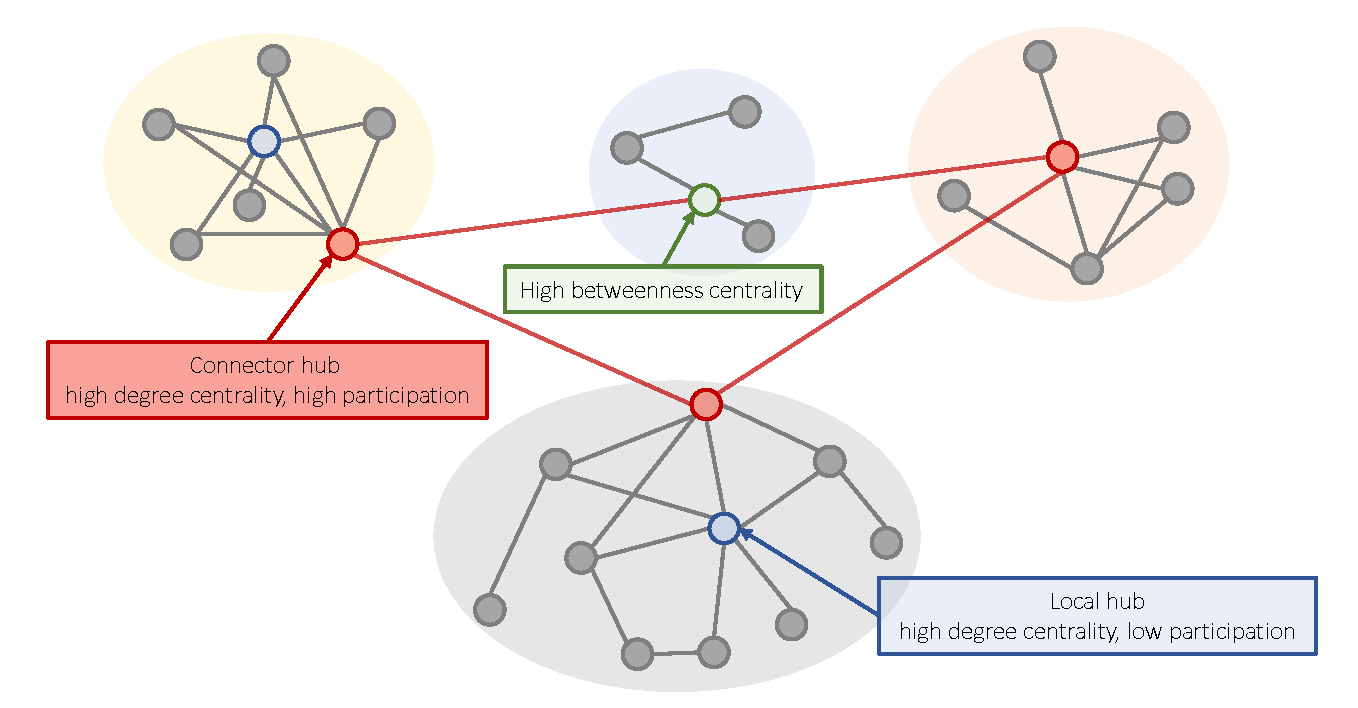
\includegraphics[width=1\textwidth]{{Chapter3/Ch3Fig1.pdf}}% This is a *.eps file
\end{center}
\caption{\textbf{Different concepts of hubness in brain networks.} A schematic representation of a modular network where nodes within a module (different background colours) show a relatively high degree of intra-modular connectivity and a low degree of inter-modular connectivity. High degree nodes can be classified into (i) local hubs (blue) that have a high degree centrality and low participation coefficient; and (ii) connector hubs (red) that have high degree and connect to nodes in other modules. Nodes with high betweenness centrality are located on shortest paths between nodes and can play an important role in linking different nodes, even if they have low degree (e.g., the green node supports communication between the yellow and orange modules).}\label{fig:Ch3Fig1}
\end{figure}

The interpretation of different measures of network centrality must be moderated by an appreciation of how the network has been constructed. If one investigates structural connectivity (e.g., through electron microscopy, tract tracing, or diffusion MRI) then network edges represent physical connections between network elements, and interpretation is straightforward. If one investigates functional connectivity (e.g., through electrophysiology, calcium imaging, or functional MRI), which captures statistical dependencies between physiological signals recorded at each node \citep{Friston1994}, the interpretation is less clear and some measures of dependence, such as the correlation coefficient, can bias the topology of the network \citep{Power2011,Zalesky2012}. Furthermore, different centrality measures make assumptions about how dynamics unfold on the network structure. For example, closeness and betweenness assume information is routed along shortest paths, which may not be a realistic model of communication in nervous systems \citep{Goni2014,Misic2015a,Seguin2018}. 

Brain network hubs are densely interconnected, forming a rich-club \citep{Colizza2006}. This property has been observed in the macroscale human connectome \citep{VandenHeuvel2011}, the mesoscale connectomes of the mouse \citep{Fulcher2016}, rat \citep{VandenHeuvel2016b}, cat \citep{DeReus2013b} and macaque \citep{Harriger2012}, and the micro-scale neuronal connectome of the \textit{C.elegans} \citep{Towlson2013} (Fig. \ref{fig:Ch3Fig2}).

\begin{figure}[h!]
\begin{center}
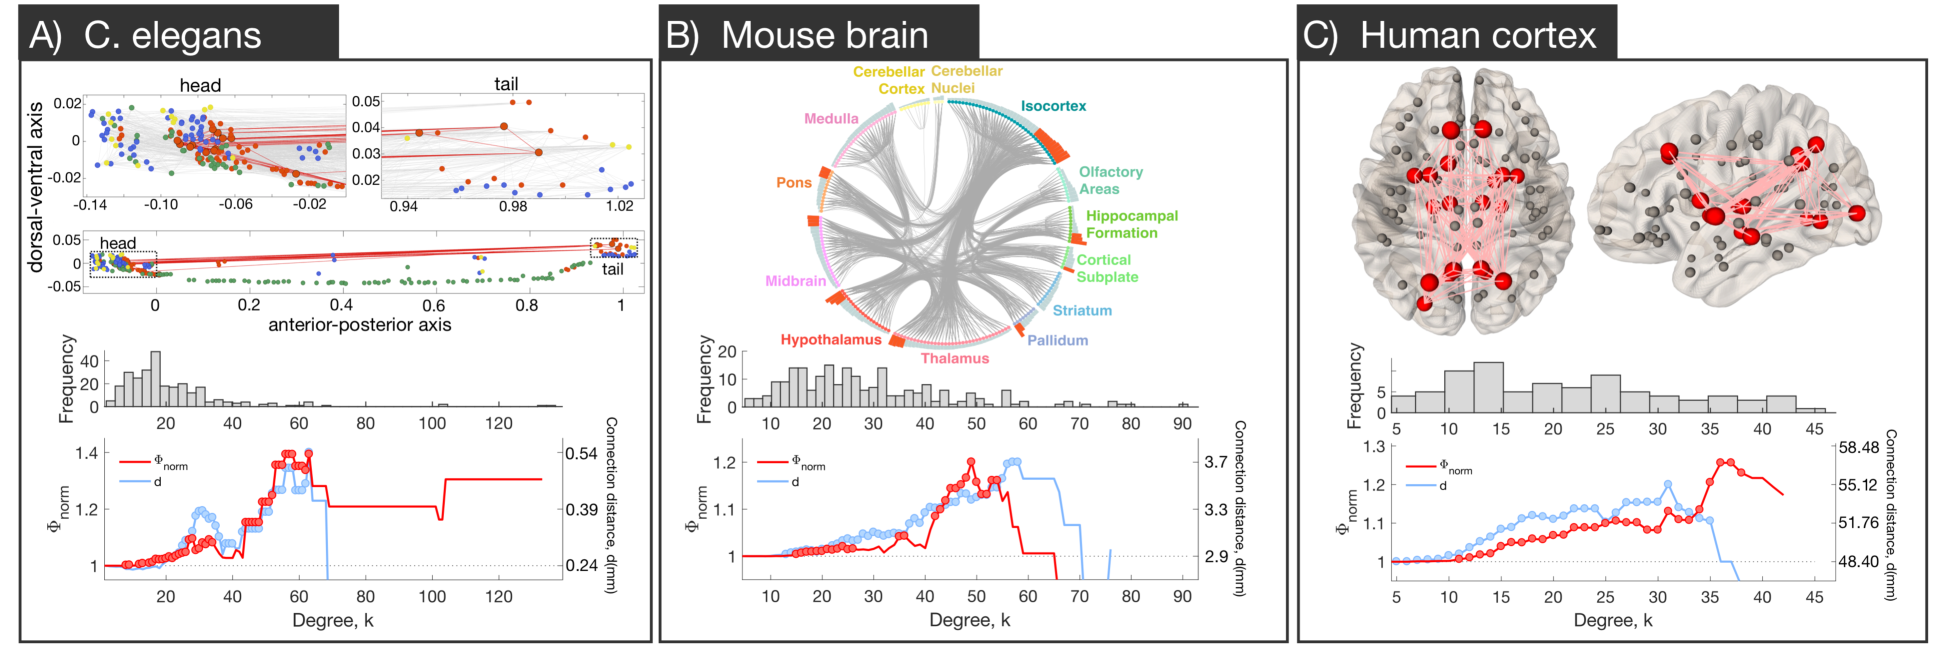
\includegraphics[width=1\textwidth]{Chapter3/Ch3Fig2.pdf}% This is a *.eps file
\end{center}
\caption{\textbf{Rich club connectivity in different species.} Top row: the spatial location of hubs in \textit{C. elegans} (A), mouse (B), and human (C). 
(A) Neurons are represented as nodes with colours corresponding to neuron type: interneurons (red), motor neurons (green), sensory neurons (blue), multimodal neurons (yellow). Hub neurons (neurons with node degree, denoted \textit{k}, greater than $44$) are shown as circles outlined in black. Connections between hubs are shown in red; other connections shown in gray in the upper plots. The upper part represents zoomed-in plots of the head and tail that are shown as dotted rectangles in the lower plot [adapted and reproduced from \citet{Arnatkeviciute2018}]. 
(B) Meso-scale connectome of the mouse. Hub regions (regions with $k > 44$) are distributed across the whole brain and contain areas in isocortex, striatum, hippocampal formation, pallidum, thalamus, hypothalamus, midbrain, pons, and cortical subplate [adapted and reproduced from \citet{Fulcher2016}].
(C) Macro-scale connectome of the human brain. Hub regions (regions with $k > 30$) are shown as big red spheres while other regions as smaller gray spheres. Connections between hubs are shown in pink. Hubs are bilateral: lingual gyrus, precuneus, superior frontal gyrus, superior parietal gyrus, insula, thalamus, putamen and hippocampus; right pallidum; left caudate and lateral occipital gyrus. 
Middle row: distribution of degree values across nodes. In each network, the distribution is heavy-tailed, consistent with the presence of highly connected hub nodes. 
Bottom row: Normalised rich club coefficient $\Phi_\mathrm{norm}$ (red) and average connection distance of hub-hub links, $d$ (blue), as a function of degree (\textit{k}) at which hubs are defined. 
The coefficient $\Phi_\mathrm{norm}$ is defined by thresholding the network at a given level of \textit{k}, calculating the density of connections between hub nodes (all nodes with degree $ > k$), and normalizing this value by the corresponding value obtained in an ensemble of appropriately matched surrogate graphs. 
The normalized coefficient therefore quantifies the degree to which the density of connections between hubs exceeds chance expectations. Since the threshold to define hubs is arbitrary, the coefficient is evaluated across all possible values of \textit{k}. 
A rise in $\Phi_\mathrm{norm}$ at high levels of \textit{k} is consistent with rich-club organization. Red circles indicate $\Phi_\mathrm{norm}$ values that are significantly higher than an ensemble of 10\,000 null networks (permutation test $p < 0.05$). 
Blue circles indicate where the mean connection distance between hubs is significantly greater relative to other links in the network (one-sided Welch’s t-test; $p < 0.05$). }\label{fig:Ch3Fig2}
\end{figure}

Given that hubs are distributed throughout the brain and involved in diverse functional systems \citep{DeReus2013b,VandenHeuvel2013a,Fulcher2016}, dense inter-connectivity of hub nodes is thought to support efficient integration of different functionally specialized systems \citep{VandenHeuvel2012}, and to increase the diversity of the brain’s functional repertoire \citep{Senden2014}. 
This integrative capacity comes at cost, with connections between hubs extending over longer anatomical distances than other types of connections \citep{VandenHeuvel2011,Harriger2012,Fulcher2016,Arnatkeviciute2018}. 
Hub regions also have the highest levels of resting metabolism \citep{Vaishnavi2010,Tomasi2013} and blood flow \citep{Liang2013a}. 
This high metabolic cost is thought to partly explain why pathology preferentially accumulates in brain network hubs across a wide range of diverse neurological diseases \citep{Bullmore2012,Crossley2014,Fornito2015}. 

The mechanisms resulting in the emergence of network hubs are unknown, but geometric constraints and evolutionary pressures to maximise adaptive function may play a role \citep{Henderson2014,Roberts2016,Betzel2017}. More generally, the striking conservation of rich-club organization across species and scales suggests that genetic influences may also play a prominent role. We now turn our attention to recent studies investigating the transcriptional correlates of hub connectivity by integrating connectomic data with spatially comprehensive gene expression databases across different species and scales. 

\section{The molecular correlates of hub connectivity}

The first study to link transcriptional measures to the hub connectivity \citep{Rubinov2015c} combined gene expression data from the AMBA \citep{Lein2007a} with a mouse connectome inferred statistically from 461 tract-tracing studies \citep{Oh2014}. 
Data from these anterograde tracer injections into the right hemisphere were aggregated into a directed and weighted connectivity matrix comprising of 112 bilaterally symmetrical cortical and subcortical nodes defining edge weights as normalised connection densities and ranging over four orders of magnitude, with $53$\% of all possible pairs of regions showing some level of non-zero connectivty. 
The authors identified a subset of nodes with high degree and a high participation coefficient, indicating that they were highly connected while also being connected to nodes in diverse functional systems. 
Using partial least squares (PLS) \citep{Herve2010}, they were able to derive a linear combination of genes whose expression levels explained $48$\% of the variance in nodal particiation coefficient. The analysis focused on a subset of 3\,380 genes form the AMBA that passed quality control criteria and were assayed in at least one additional independent experiment allowing the authors to evaluate gene expression reproducibility. The genes weighting strongly on the participation-related component were enriched for GO categories such as learning, cognition, and memory, suggesting a link between the expression of genes related to regional variations in network participation and those implicated in cognition. 

In a subsequent analysis of the Allen Institute mouse connectome, Fulcher and Fornito (2016) used a parcellation comprising $213$ regions linked by $3\,063$ connections ($6.9$\% of all possible links), focusing on the right hemisphere only (where complete information on afferent and efferent connectivity was available), in combination with ISH measures of expression across $17\,642$ genes in the AMBA \citep{Lein2007a}. 
Their primary aim was to characterize how coupled patterns of gene expression between regions (i.e., correlated gene expression or CGE) relate to network topology. After confirming that the right hemisphere of the mouse connectome did indeed show evidence of rich-club organization, and that connections between hubs were both the most costly (measured by connection distance, reciprocity and weight) and central (measured using edge betweenness centrality and an alternative measure called communicability, that does rely on shortest path communication) connections of the network, they distinguished between three topological classes of connections following the work of \citet{VandenHeuvel2012}: (i) rich links, which connect two hubs (where hub is defined based on degree); (ii) feeder links, which connect a hub to non-hub (feed-out) or a non-hub to a hub (feed-in); 
and (iii) peripheral links, which connect two non-hubs (Figure \ref{fig:Ch3Fig3}A). 
Across a wide range of thresholds for defining a hub, CGE was highest for rich links, followed by feeder, and lowest for peripheral edges, with CGE showing a sharp rise at a hub threshold range that coincided with a regime in which a significant topological rich club was observed (Figure \ref{fig:Ch3Fig3}B). This tightly coupled transcriptional activity between hub nodes defied a general trend in the brain where CGE between two areas decayed sharply (exponentially) as a function of their distance. That is, despite connected hubs being separated by longer anatomical distances than other pairs of regions, they showed the highest levels of transcriptional coupling (note that CGE measures were corrected for this dependence). 
Enrichment analysis showed that this effect was driven by genes regulating the oxidative synthesis and metabolism of ATP---the primary energetic source of neuronal communication. By comparison, an enrichment analysis comparing connected to unconnected regions (regardless of whether those connections involved hubs) found significant involvement of a large number of GO categories related to synaptic plasticity and communication, axon structure, and metabolism. These findings suggest that while genes involved in forming and maintaining synapses and axons are important for establishing a connection between two regions, the primary genomic distinction between different topological classes of connections (as defined in relation to hubs) is related to the metabolic requirements of those connections.

More recently, we found a qualitatively similar pattern of elevated CGE in rich links in the nematode \textit{C. elegans} connectome \citep{Arnatkeviciute2018}. 
Combining electron micrograph data defining the electrochemical connectome of 279 neurons \citep{Varshney2011} with binary gene expression profiles across 948 genes (Figure \ref{fig:Ch3Fig3}C) acquired from WormBase \citep{Harris2010}, we identified the same trend for CGE to be highest for rich links, followed by feeder, and then peripheral edges (Figure \ref{fig:Ch3Fig3}D). 
The involvement of metabolic genes in rich-club connectivity---as in the mesoscopic mouse connectome \citep{Fulcher2016}---could not be confirmed due to limited gene expression data in the worm, but analysis of the available data indicated that glutamate signalling and neuronal communication genes made the strongest contribution to elevated CGE for hub-hub connections \citep{Arnatkeviciute2018}. 
Leveraging the extensive additional data on neuronal phenotypes available for the worm, we found that elevated CGE for connected hubs could not be explained by a range of other properties such as neuronal lineage distance (number of cell divisions separating pairs of neurons from a common ancestor), differences in birth time, neuronal subtype (sensory, motor, or interneuron), chemically secreted neurotransmitter, anatomical separation distance or topological module affiliation. However, the effect did seem to be driven by the fact that most hubs in the worm connectome are command interneurons, a specialized class of neurons that regulates motion. Motion is one of the more complex behaviors in the worm’s repertoire, and these findings parallel evidence in primates that network hubs are primarily located in association cortices, which are thought to mediate higher-order cognition \citep{Achard2006,Sporns2007}. 
Thus, despite numerous differences in the data, including different gene annotation methods ($\sim20\,000$ ISH genes in mouse versus $\sim1\,000$ binary literature-curated annotations in worm), the type of the neural system (spatially continuous macroscopic mouse brain \textit{vs} spatially separated \textit{C. elegans} nervous system), and the orders of magnitude differences in scale, both studies demonstrated the same general pattern of increased transcriptional similarity across topologically central hub nodes.

\begin{figure}[!h]
\begin{center}
\includegraphics[width=1\textwidth]{Chapter3/Ch3Fig3.pdf}% This is a *.eps file
\end{center}
\caption{\textbf{Empirical studies investigating the transcriptional properties of hub connectivity in mouse (A,B) and \textit{C. elegans} (C,D).} 
(A) The schematic representation of different types of connections in the mouse brain: rich (connecting a hub to a hub)---red, feeder (connecting a hub to a non-hub or a non-hub to a hub)---green, peripheral (connecting a non-hub to a non-hub)---blue. Links in the connectome were categorized across this scheme. For each region, a vector of gene expression values was extracted as the corresponding row of the region in the full gene expression matrix comprising the AMBA. The matrix represents the normalised gene expression of $17\,642$ genes (columns) across $213$ regions (rows). Gene expression profiles for each region were then used to estimate correlated gene expression (CGE) between region pairs. 
(B) Mean correlated gene expression for rich, feeder and peripheral links as a function of node degree (\textit{k}) where hubs are nodes with degree $> \textit{k}$. The mean CGE of rich links increases at levels of \textit{k} that coincide with a regime where evidence of topological rich-club organization is found indicating that CGE is highest for connected pairs of network hubs. The topological rich club regime (determined from the network topology, see Fig. \ref{fig:Ch3Fig2}A) shaded gray. Circles indicate a statistically significant increase in correlated gene expression for a given link type relative to the rest of the network (one-sided Welch-s t-test; $p < 0.05$) [adapted and reproduced from \citet{Fulcher2016}]; 
(C) Neuron-and-synapse connectome of \textit{C. elegans}, reconstructed for $279$ neurons using electron microscopy. Connections coloured according to how they connect hubs (neurons with degree $> 44$) and non-hubs (neurons with degree $≤ 44$): red (rich links connecting hubs), orange (feed-in links connecting a non-hub to a hub), yellow (feed-out links connecting a hub to a non-hub), blue (peripheral links connecting non-hubs). Middle: additional data acquired for each neuron such as its: chemically secreted transmitter, anatomical location, birth time, hub status and neuronal type. Right binary gene expression profile for each of the $279$ neurons (rows) across $948$ genes (columns).
(D) Median CGE for each connection type (feed-in and feed-out connections are combined and represented as feeder) as a function of node degree \textit{k}. The topological rich club regime (determined from the network topology, see Fig. \ref{fig:Ch3Fig2}A) shaded gray. 
Circles indicate a statistically significant increase in CGE in a given link type relative to the rest of the network (one-sided Wilcoxon rank sum test, $p < 0.05$) [adapted and reproduced from \citet{Arnatkeviciute2018}]. } \label{fig:Ch3Fig3}
\end{figure}


In light of the findings in both mouse and \textit{C.elegans}, where several groups of genes implicated in cognition \citep{Rubinov2015c}, oxidative metabolism \citep{Fulcher2016}, and neuronal communication \citep{Arnatkeviciute2018} have been identified as being related to hub connectivity, one could wonder whether the same genes are involved in the hub connectivity of the human brain. The first analysis to link gene expression and hub connectivity in humans was performed by \citet{Vertes2016b}, who combined resting-state fMRI (rs-fMRI) data with the high coverage genome-wide gene expression from AHBA \citep{Hawrylycz2012}. 
Rendering rs-fMRI data for $285$ cortical regions as a binary undirected network, thresholded to retain $10$\% of all possible connections, they measured three different properties of each node: its within-module connectivity, its participation coefficient (between-module connectivity), and its average Euclidean distance from other nodes. 
PLS identified three components that collectively accounted for $37$\% of the total variance in nodal metrics with the first component exhibiting a positive correlation with intra-modular degree and a negative correlation with average nodal distance, corresponding to high degree nodes that mostly form short-range within-module connections. Genes positively loading on this component were enriched for GO categories related to transcriptional regulation. The second component was positively related to both the participation coefficient and average nodal distance, thus representing nodes with long connections that extend between modules, consistent with the integrative hubs of the network (Figure \ref{fig:Ch3Fig4}A).
As seen in the analysis of the structural connectivity analysis of the mouse \citep{Fulcher2016}, genes loading positively on this component were enriched in GO categories related to oxidative metabolism and mitochondrial function.  
These genes also showed significant overrepresentation for a set of $19$ genes \citep{Krienen2016} selectively enriched in the supragranular layers of the human cortex (HSE – human supragranular enriched genes) with some of those genes being implicated in the formation of corticocortical projections emanating from the higher layers of the cortex \citep{Krienen2016}. 
Together these findings suggest that hubs across species demonstrate conserved transcriptional properties related to their high metabolic demands.

It is well-known that the human brain undergoes an extended period of development during adolescence that is critical for brain maturation and coincides with the period of peak risk for many mental disorders \citep{Paus2008}. Some of those developmental changes particularly target hub regions \citep{Dennis2013,Hwang2013,Baker2015a} [for a review see \citep{Cao2016}]. 
\citet{Whitaker2016a} examined a large sample of adolescents (279, aged 14 to 24 years old) and found that topologically central hubs of the cortical structural covariance networks undergo an increased rate of consolidation, defined by increased cortical thinning and enhanced myelination (Figure \ref{fig:Ch3Fig4}B).
Components of transcriptional variance that correlated with this consolidation were extracted using PLS, employing the full set of 20\,737 genes from the AHBA. The first two components explaining 28\% of the variance in MRI measures were related to the baseline measures of cortical thickness and myelination (PLS1), and cortical shrinkage and myelination - consolidation over time (PLS2) (Figure \ref{fig:Ch3Fig4}B) respectively. 
The PLS2 component involved contributions from genes regulating synaptic transmission and a set of genes linked to risk for schizophrenia, suggesting that deviation from the normal developmental consolidation of hub regions might manifest as an intermediate phenotype for schizophrenia \citep{Whitaker2016a}, consistent with evidence that hubs are disproportionately impacted by the disease \citep{VanDenHeuvel2013,Crossley2014,Klauser2016} and that regional variations in the expression of schizophrenia risk genes track the regional variations in the magnitude of group differences in connectivity between controls and patients \citep{Romme2017}. 

\begin{figure}[H]
\begin{center}
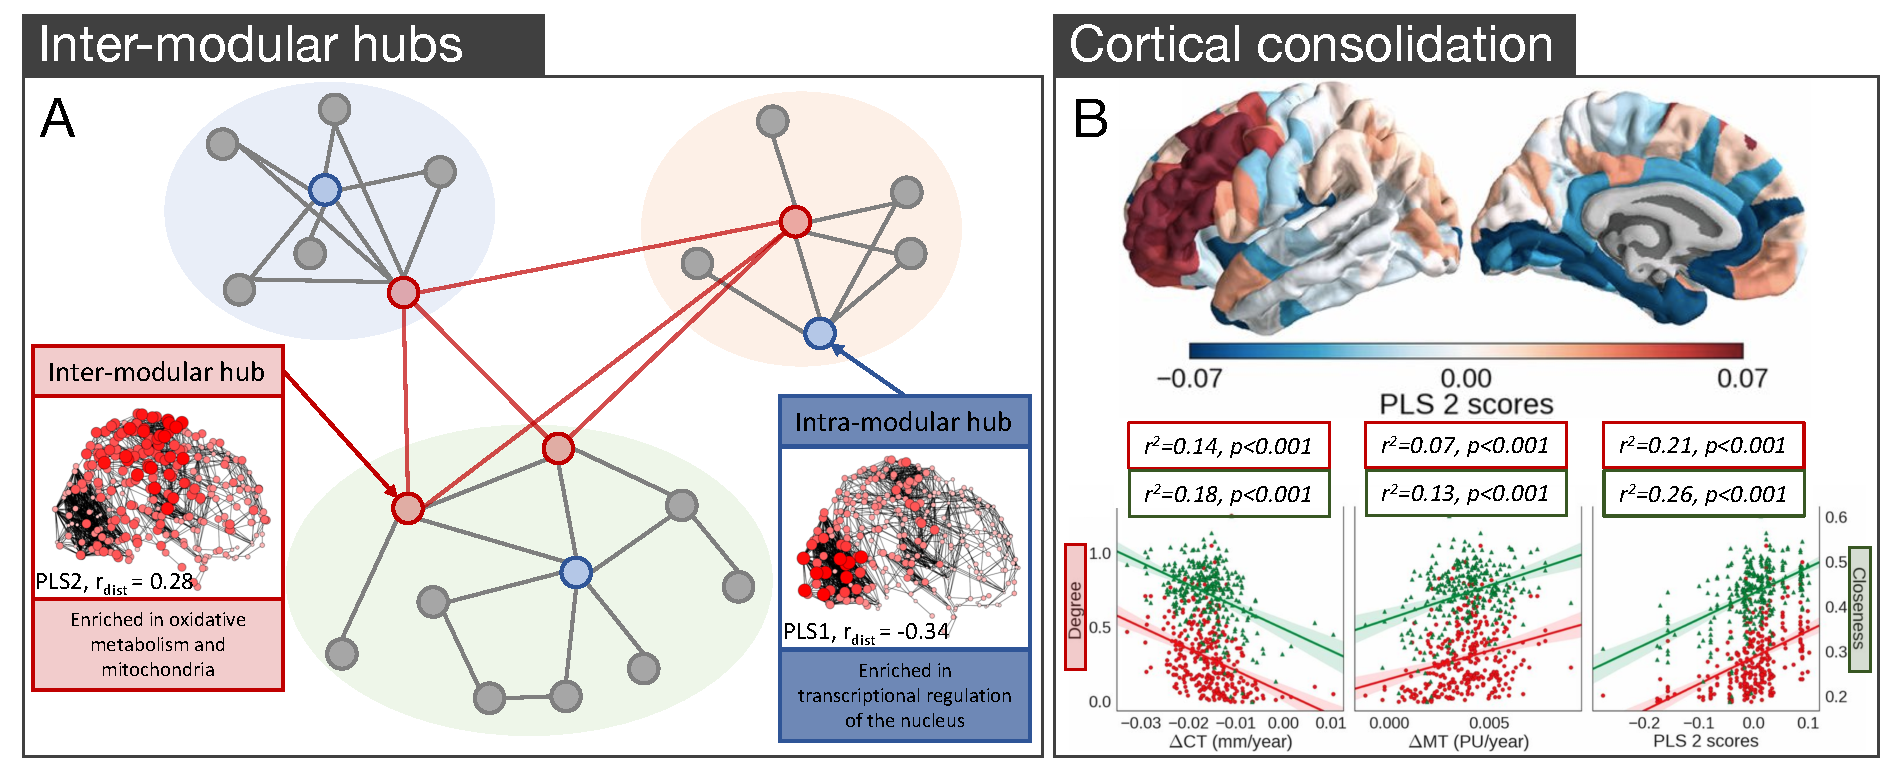
\includegraphics[width=1\textwidth]{Chapter3/Ch3Fig4.pdf}% This is a *.eps file
\end{center}
\caption{\textbf{Empirical studies investigating the transcriptional properties of hub connectivity in human.} 
(A) A schematic representation of the modular organization of the connectome demonstrating the key properties of inter- and intra- modular hubs based on \citet{Vertes2016b}. 
Intra-modular hubs (blue nodes) mostly connect nodes within the same module and are characterized with a relatively short connection distances; characterized by the PLS1. Intra-modular hubs (red nodes) have a more diverse connectivity profile with connections extending long distances and connecting nodes from different modules; characterized by the PLS2. Size and color saturation of the nodes in the connectome corresponds to the regional scores on PLS1 (Intra-modular hub) and PLS2 (Inter-modular hub) to represent the spatial pattern of transcriptional profiles [adapted and modified from \citet{Vertes2016b}]. 
(B) Gene expression and cortical consolidation in adolescence based on \citet{Whitaker2016a}, 
top: spatial topography of the second component from a PLS analysis corresponding to cortical consolidation during adolescence, defined as cortical shrinkage/myelination. Genes identified in this profile are related to synaptic transmission and risk to schizophrenia, among others, and are overexpressed in prefrontal areas of the cortex; bottom: hubs in the structural covariance network experience faster rates of cortical thinning (CT) and myelination. The PLS2 gene expression profile is also significantly associated with degree, meaning that hubs are likely to over-express those genes [adapted and modified from \citet{Whitaker2016a}]. } \label{fig:Ch3Fig4}
\end{figure}

Importantly, this work implies that genes involved in the development of hubs, which relate to myelination and synaptic transmission, are distinct from those implicated in cross-sectional studies of adult hub connectivity, which implicate metabolic genes. In other words, the genetic mechanisms underlying the development of hub connectivity may differ from those involved in sustaining the functional role that hubs play in a mature neuronal system. The further development of brain-wide atlases of developmental changes in gene expression will help shed light on how such differences can be leveraged to gain insight into the development of different brain disorders.

\section{Conclusions and further directions}

Brain-wide gene expression atlases provide exciting opportunities to link different scales of brain organisation. At the same time, integrating such data with connectomic measures poses challenges. Given the nascense of this field, no standardized data processing pipelines have been developed, with widespread inconsistencies in processing of the same transcriptional data across studies \citep{Arnatkeviciute2019} complicating direct comparison between findings, even within the same species. Nonetheless, the available studies---conducted in diverse species and using different measures of brain connectivity and gene expression acquired at different resolution scales---point to a conserved transcriptional signature of hub connectivity related to genes regulating neuronal communication and metabolism, consistent with the high centrality and metabolic cost of hub regions \citep{Bullmore2009}.

One limitation affecting the human data is that the gene expression measures are derived from bulk tissue samples. The cellular composition of these samples can influence measured gene expression patterns, such that two samples can differ in their transcriptional properties simply due to the differences in the density of distinct cell types. Single-cell transcriptomics is able to provide precise gene expression measurements in individual cells, thus resolving cell-specific transcriptional profiles. While scRNA-seq is not currently feasible for the whole human brain, the expression profiles of specific cell groups in the adult \citep{Johnson2015a,Hu2017,Picardi2017} and developing brain \citep{Zhong2018} are being characterized. 

These limitations notwithstanding, the consistency of results considered here---often identified through unbiased, data-driven techniques--- demonstrate the potential utility of brain-wide transcriptomic measures in yielding biologically meaningful insights to otherwise abstract graph-theoretical structures such as hubs and other neural phenotypes. With the availability of new resources and developments in neuroimaging, the combination of such data across resolution scales offers a promising way forward for uncovering the molecular mechanisms that drive the large-scale organization of the connectome.

\section*{Acknowledgments}

We would like to thank Stuart Oldham for processing human DWI data used in Figure \ref{fig:Ch3Fig2}. 
  
  \clearpage
  %!TEX root = ../Thesis.tex
\chapter{Linking brain-wide gene expression and neuroimaging data}
\label{ch:Chapter4}
\fancyhead[R]{\textit{Chapter.} \textit{\thechapter: }\textit{Linking brain-wide gene expression and neuroimaging data}}


% Insert author names, affiliations and corresponding author email (do not include titles, positions, or degrees).

\textbf{Aurina Arnatkevi\u{c}i\={u}t\.{e}},
Ben D. Fulcher,
Alex Fornito (2019).
A practical guide to linking brain-wide gene expression and neuroimaging data. Published in \textit{NeuroImage}.\\
DOI: \url{https://doi.org/10.1016/j.neuroimage.2019.01.011}

\section*{Preamble}
The Allen Human Brain Atlas (AHBA) provides an unprecedented brain-wide gene expression database that can be used in combination with a range of brain imaging methods to map the transcriptional markers of imaging-derived phenotypes. In this thesis we use the AHBA to investigate transcriptional markers of hub connectivity, however, inconsistencies in methods used for processing the AHBA data throughout the literature led us to question the impact of different approaches employed. In this chapter we propose a seven-step processing pipeline for integrating AHBA and neuroimaging data and compare the influences of different methodological choices, making the first step towards a standardized analysis pipeline that can be routinely employed throughout the field and benefit the reproducibility. This groundwork was a necessary precursor for the following analyses presented in Chapter 5.\\
Supplementary materials for this chapter are in Appendix \ref{appendixB}.

\newpage

\section*{Abstract}
The recent availability of comprehensive, brain-wide gene expression atlases such as the Allen Human Brain Atlas (AHBA) has opened new opportunities for understanding how spatial variations on the molecular scale relate to the macroscopic neuroimaging phenotypes. A rapidly growing body of literature is demonstrating relationships between gene expression and diverse properties of brain structure and function, but approaches for combining expression atlas data with neuroimaging are highly inconsistent, with substantial variations in how the expression data are processed. The degree to which these methodological variations affect findings is unclear. Here, we outline a seven-step analysis pipeline for relating brain-wide transcriptomic and neuroimaging data and compare how different processing choices influence the resulting data. We suggest that studies using AHBA should work towards a unified data processing pipeline to ensure consistent and reproducible results in this burgeoning field.

\section{Introduction}

Over the past two decades, human imaging genetics has emerged as a powerful strategy for understanding the molecular basis of macroscopic neural phenotypes measured across the entire brain \citep{Meyer-Lindenberg2006a,Munoz2009,Arslan2015,Hashimoto2015}. Traditionally, this work has involved correlating allelic variation at one or more genetic loci with variation in one or more imaging-derived phenotypes (IDPs), initially through candidate gene studies and more recently at a genome-wide level. The latter has been facilitated by the formation of large consortia, such as ENIGMA \citep{Thompson2014}. A common assumption in this work is that variants associated with an IDP (or nearby variants tagged by the associated variant) influence gene expression or protein abundance, which in turn alters cellular function and ultimately affects the studied IDP. However, multiple environmental and other factors can impact gene activity \citep{Fraser2005,Choi2007,Cole2009} and the functional roles of many IDP-linked variants, which are usually identified through large-scale statistical analyses, are often unknown. As a result, the mechanisms through which a given variant may influence phenotypic variation can be unclear. Moreover, the expression levels of many genes vary substantially across brain regions \citep{Hawrylycz2015}, and these spatial variations cannot be inferred from DNA sequence alone.

Assays of gene expression provide a more direct measure of gene function. Expression assays are invasive, requiring direct access to neural tissue, and technical limitations have historically constrained analyses of gene expression in the brain to small sets of areas studied in isolation. Recent advances in the development of high-throughput tissue processing and bioinformatics pipelines have overcome these limitations, resulting in datasets of gene expression across a large fraction of the genome in a large number of brain regions, and through various stages of development [see \citet{Keil2018} for a detailed overview]. While some of the human atlases span multiple brain areas, only the Allen Human Brain Atlas (AHBA) offers high resolution coverage of nearly the entire brain, comprising expression measures for more than \num{20000} genes taken from \num{3702} spatially distinct tissue samples. Critically, the samples have been mapped into the stereotaxic space, allowing researchers to directly relate spatial variations in gene expression to spatial variations in IDPs (for more details on the AHBA see \ref{app:AppendixCh4_1}).

This unprecedented capacity to link molecular function to macroscale brain organization has given rise to the nascent field of imaging transcriptomics [for an overview, see \citep{Fornito2019}], which has begun to yield new insights into how regional variations in gene expression relate to: functional connectivity within canonical resting-state networks \citep{Richiardi2015,Forest2017};
fiber tract connectivity between brain regions \citep{Goel2014};
temporal and topological properties of large-scale brain functional networks \citep{Cioli2014b,Vertes2016b};
the specialization of cortical and subcrotical areas \citep{Krienen2016,Parkes2017,Anderson2018};
regional maturation during embryonic and adolescent brain development \citep{Kirsch2016a,Whitaker2016a};
and pathological changes in brain disorders \citep{Rittman2016,Romme2017,McColgan2018,Romero-Garcia2018a}. Software toolboxes to facilitate the integration of brain-wide transcriptomic and imaging data have also been developed \citep{French2015,Gorgolewski2015,Rizzo2016,Rittman2017}.

Unlike behavioral genetics or studies of structural DNA variants, where the goal is to understand how genetic variation correlates with phenotypic variability across a sample of individuals, analyses in imaging transcriptomics are concerned with identifying spatial correlations between gene expression patterns and some property of brain structure or function \citep{Fornito2019}. In other words, the goal is to identify genes with spatial profiles of expression that track anatomical variations in a given IDP. These analyses are often highly multivariate, involving expression measures of around \num{20000} genes in each of around $10^{2}$-$10^{3}$ brain regions, being related to one or more distinct IDPs quantified in each region. This complexity is compounded by the fact that both imaging data and gene expression data undergo extensive processing prior to analysis.

The impact of data processing choices on the results of neuroimaging analyses is well documented, with strategies for the correction of motion-related and global signal fluctuations in functional MRI being a prime example \citep{Power2015a,Power2017,Ciric2017,Parkes2018}. Comparable scrutiny has not yet been applied to the many processing choices that can affect the analysis of transcriptomic atlases and their relation to IDPs. At the time of writing, more than 30 studies have linked the AHBA gene expression measures to human neuroimaging data. The lack of a standard processing pipeline for gene expression data means that the degree to which the results of this work are robust to different methodological choices remains unclear.

As the field develops, it is important to establish methodological guidelines to ensure consistent and reproducible results, and to support valid interpretation. In this paper, we offer a practical guide to some of the key steps in processing the AHBA gene expression data and examine the potential impact of methodological choices available at each step. We focus on the AHBA, as it is the most spatially comprehensive and widely used gene expression atlas in the field \citep{Hawrylycz2012}.

The paper is organised as follows. We begin by summarizing some basic aspects of how gene expression is quantified, and general characteristics of the AHBA. We then outline several key steps in a basic workflow for relating gene expression measures to imaging data and examine the impact of methodological choices at each step. In the final section, we make some recommendations for best practice and provide directions for further research.


\section{Measuring gene expression}

Gene expression is a process through which genetic information encoded by sequences of DNA is read and used to synthesize a particular gene product, such as a protein or RNA molecule \citep{Szymanski2002}. The order of amino acids within each gene determines the structure and function of the resulting product, which in turn affects cellular function and drives phenotypic variability. While the DNA sequence of each cell in the organism is identical, different cells and anatomical structures express different phenotypes (e.g., neurons versus lymphocytes) due to differences in gene expression. The process through which a sequence of DNA is expressed is complex, but (for present purposes) can be divided into two main stages: (1) transcription, which occurs when an unwound segment of DNA is read to produce messenger RNA (mRNA); and (2) translation, which occurs when mRNA is used to synthesize proteins \citep{Krebs2014}. Gene expression is commonly approximated by measuring mRNA levels of a particular gene and is thus an index of gene transcriptional activity. Gene transcription is an indirect proxy for protein abundance, which is ultimately determined by gene translation. This distinction is important as several studies have shown that mRNA and protein levels within a tissue can vary significantly \citep{Futcher1999,Gygi1999,Greenbaum2003}, and gene expression (transcriptional activity) and protein abundance (translational activity) are not always positively correlated \citep{Margineantu2007,Schwanhausser2011}.

In the AHBA, transcriptional activity has been measured using microarray, which quantifies the expression levels of thousands of genes at once by measuring the hybridization of cRNA (Cy3-labeled RNA) in a tissue sample to a  particular spot on the microarray chip. Each of these spots, called probes, maps to a unique location of the DNA and contains single-stranded nucleic acid profiles that are ready to anneal to their complementary targets in the process of hybridization. Relative levels of gene expression in a tissue sample are then quantified by measuring the fluorescence at each sequence-specific location, which is proportional to the amount of cRNA in a sample \citep{Tarca2006}. This method provides a cost-effective way to measure gene expression in high-throughput manner. However, it is limited to known gene sequences, is prone to background noise due to indirect assessment of expression values, and spatial biases can result from variability in the lateral diffusion of target molecules on the chip \citep{Steger2011}. Expression measures can also be affected by cross-hybridization artefacts arising when cRNA anneals to an imperfectly matched probe.

Microarray is typically performed on bulk tissue samples, and the cellular composition of a sample can strongly influence its gene expression profile. As a result, two samples with varying densities of different cell types may show transcriptional differences simply because of their different cellular composition. This is an important consideration when comparing data acquired from samples taken from different parts of the brain, since variations in the density of distinct cell types may drive differences in regional gene expression. In addition, variations in the way tissue samples are acquired, handled and processed, age at death \citep{Glass2013}, sex \citep{Berchtold2008,Trabzuni2013}, ethnicity \citep{Spielman2007}, brain pH \citep{Mexal2006}, post-mortem interval \citep{Zhu2017}, and RNA degradation \citep{Jaksik2015}, can all affect expression measures. Another potential influence arises from batch effects, caused by samples being processed at different times, by different staff, or in different labs; even changing atmospheric ozone levels can impact the final measures \citep{Fare2003} [see \citet{Scherer2009} for an overview]. The Allen Institute has implemented a series of steps to mitigate this variability as much as possible, as outlined in Allen Human Brain Atlas technical white paper \citep{AHBAdoc}.

One final consideration is that any individual gene expression assay provides a static snapshot of a dynamic process. Gene expression changes through development, and as a function of experience, environmental exposures and other factors \citep{Fraser2005,Choi2007,Berchtold2008,Cole2009,Birdsill2011,Naumova2012,Kumar2013}.
The further advancement of developmental atlases of gene expression \citep{Johnson2009,Colantuoni2011,Kang2011,Fertuzinhos2014,Bakken2016} will help to shed light on these dynamic processes.

% METHODS: connectivity data
\section{A general workflow for processing brain-wide transcriptomic data}
The AHBA consists of microarray data in \num{3702} spatially distinct samples taken from six neurotypical adult brains. The samples are distributed across cortical, subcortical, brainstem and cerebellar regions in each brain, and quantify the expression levels of more than \num{20000} genes (for more details see \ref{app:AppendixCh4_1}). Different brain regions were sampled across each of the six AHBA donors to maximize spatial coverage. Figure \ref{fig:Ch4Fig1} shows the  variability of coverage across individual brains.

Each tissue sample is associated with a numeric structure ID, name and structure label (cortex, cerebellum, or brainstem) in addition to the MRI voxel coordinates in native image space and MNI stereotaxic coordinates, which can be used to match samples to other imaging data (Figure \ref{fig:Ch4Fig1}). The AHBA also provides: (1) a binary indicator of when the level of a given transcript exceeds background levels, which can be used for quality control purposes; (2) RNA-seq data for a subset of tissue samples in two donor brains (120 samples each), which can be used for cross-validating expression measures (as we show below); and (3) magnetic resonance images, including T1-weighted, T2-weighted, T2-weighted gradient echo and FLAIR scans for all six brains, and diffusion-weighted images for two brains. These scans were collected prior to the dissection for anatomical visualization.

\begin{figure}[h!]
  \centering
    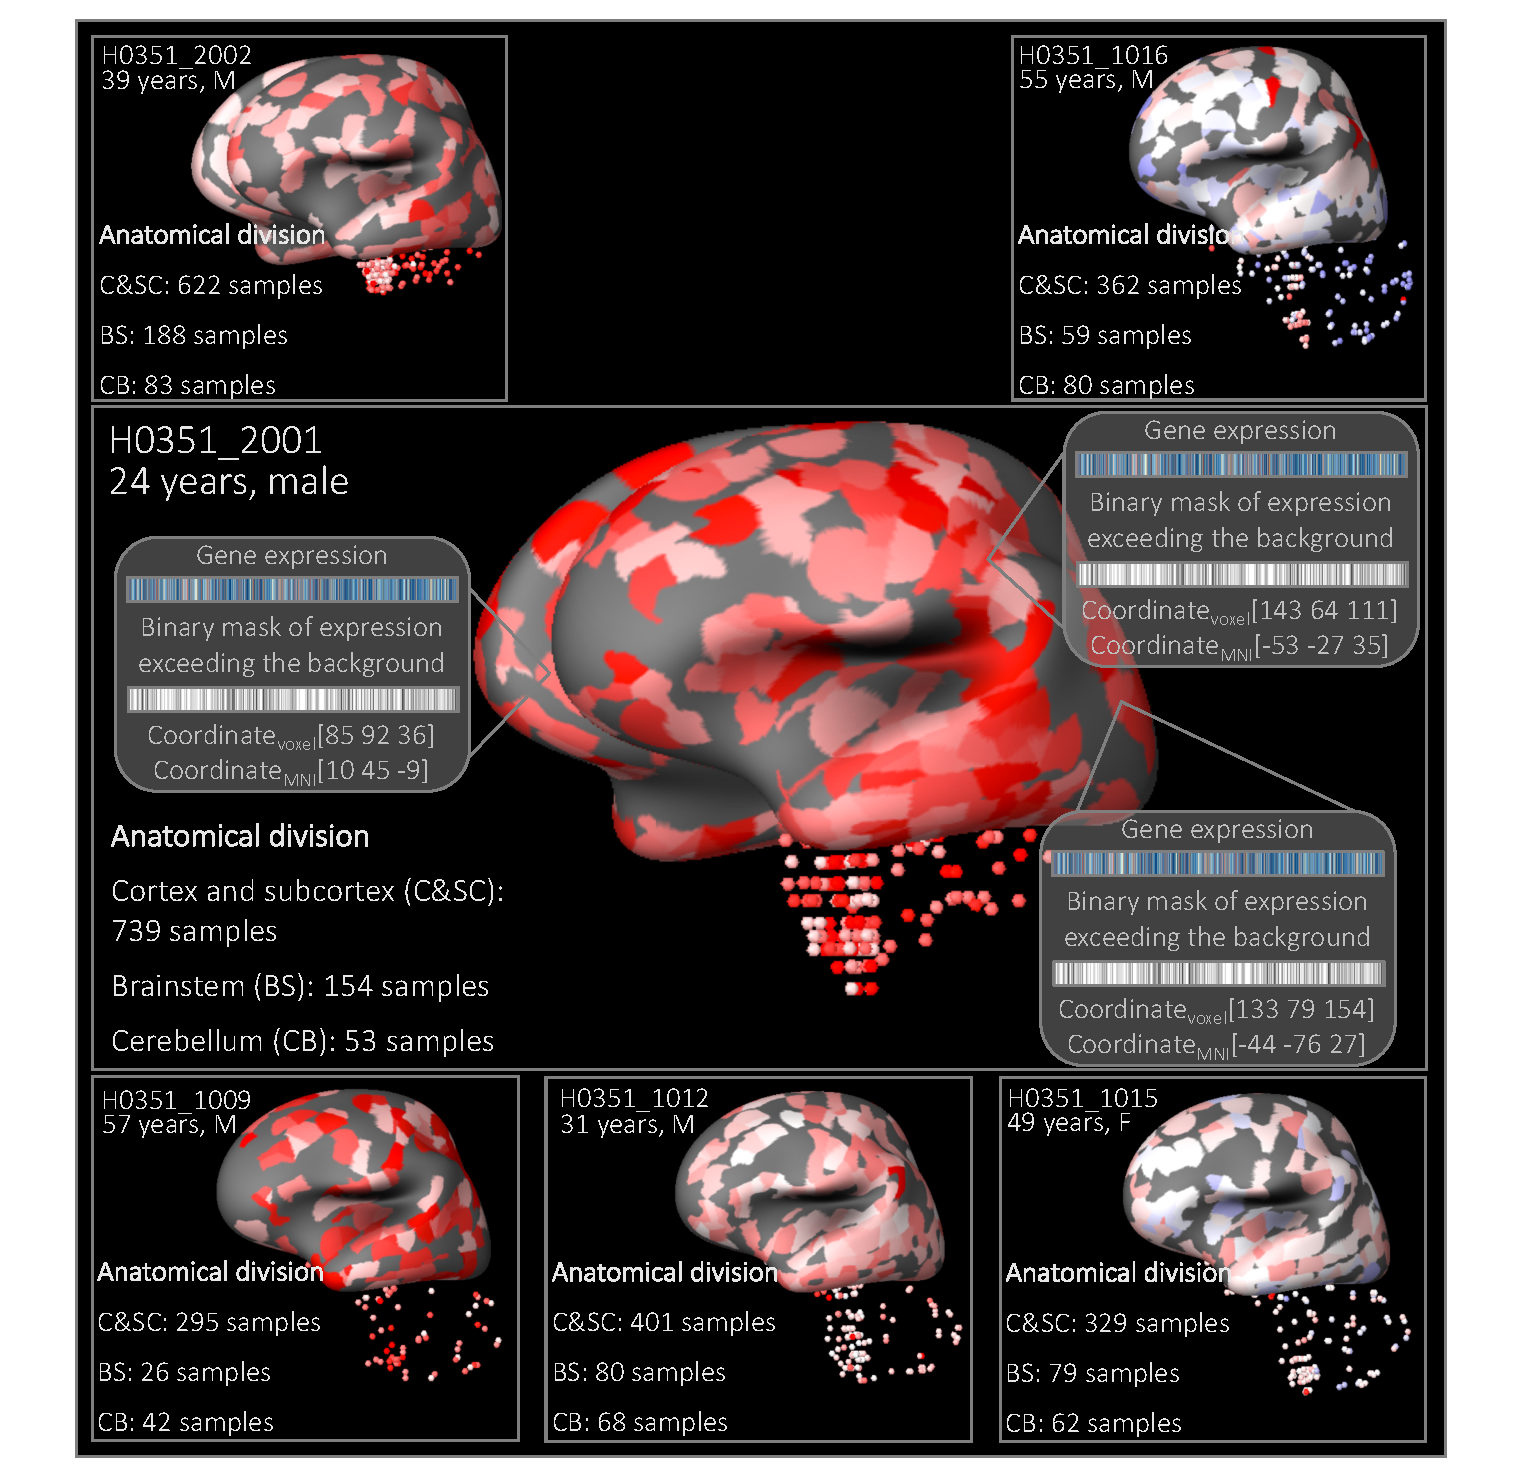
\includegraphics[width=1\textwidth]{Chapter4/Ch4Fig1.pdf}
\caption{\textbf{A schematic representation of expression data for a selected representative gene: CLRN1}. Discrete tissue samples in each brain are represented as colored areas on a grey brain surface. Color corresponds to the gene expression level of each sample relative to all other samples combined over all six brains ($z$-score): red (high), blue (low). The size of the patch is not representative of the size of the actual tissue sample used to quantify gene expression (which was much smaller than shown). The patch has been padded out by the AHBA online platform as a visual aid. The number of samples in each anatomical division: cortex and subcortex (C\&SC), brainstem (BS) and cerebellum (CB) for every donor brain is listed. Middle: A schematic representation of available data for each sample which includes expression values for $\sim$\num{20000} genes, a binary indication of whether the expression levels exceed background noise, and native voxel and MNI coordinates for each sample. Brain representation produced using Brain Explorer 2 (2006-2015 Allen Institute for Brain Science; available from: \url{http://human.brain-map.org/static/brainexplorer}). }
\label{fig:Ch4Fig1}
\end{figure}

The AHBA samples were processed over approximately three years, which raises concerns about possible batch effects. Expression data were subjected to normalization procedures within a single brain, as well as between brains, to minimize the effect of non-biological biases such as array-specific differences, dissection method, and RNA quality differences among others, while maintaining biologically-relevant variance. Detailed information about the normalization is provided in the technical white paper \citep{AHBAdoc}. Despite these procedures, we show below that large inter-individual differences in gene expression remain, such that samples from the same brain tend to have more similar gene expression compared to the samples from other brains. These differences must be taken into account when combining data across all six brains.

Beyond the processing steps applied by the Allen Institute, a number of other procedures are required to link expression measures and neuroimaging data. Here we outline seven major steps, summarized in Figure \ref{fig:Ch4Fig2}, which represent the core features of a typical workflow:
(i) verifying probe-to-gene annotations;
(ii) filtering of probes that do not exceed background noise;
(iii) probe selection, where representative probes (or a summary measure) are selected to index expression for a gene;
(iv) sample assignment, where tissue samples from the AHBA are mapped to specific brain regions in an imaging dataset;
(v) normalization of expression measures to account for inter-individual differences and outlying values;
(vi) gene-set filtering, to remove genes that are inconsistently expressed across six brains and/or to select genes in a hypothesis-driven way based on the research question.
(vii) accounting for the spatial patterns in gene expression;

The first six processing steps produce the region $\times$ gene matrix that can be used for the regional analyses.
The final step of accounting for the autocorrelation in the gene expression measures depends on the particular research question.
The potential need to account for spatial effects arises because gene expression is more strongly correlated between samples that are separated by short distances compared to those that are far apart, a pattern that has been described in humans
\citep{Richiardi2015,Krienen2016,Vertes2016b,Pantazatos2017}, mouse \citep{Fulcher2016} and \textit{C.elegans} \citep{Arnatkeviciute2018}.
Although this spatial autocorrelation is, in itself, an important neurobiological feature of the brain transcriptome \citep{Gryglewski2018, Fornito2019},
it is critical for any analysis claiming a specific association between spatial variations in gene expression and a given IDP to show that the association is not attributable to lower-order spatial gradients of gene expression.

In the following sections, we outline some of the choices that can be made at each of these steps and consider their impact on analysis with some recommendations summarized in the conclusions section. Code and data are available at github \url{https://github.com/BMHLab/AHBAprocessing} and figshare \url{https://doi.org/10.6084/m9.figshare.6852911} respectively.

\begin{figure}[h!]
  \centering
    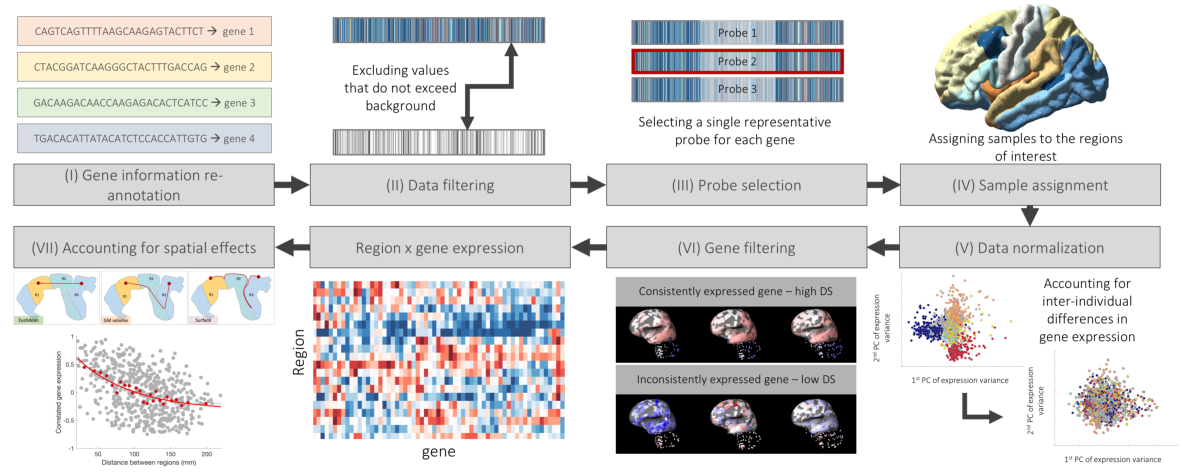
\includegraphics[width=1\textwidth]{Chapter4/Ch4Fig2.pdf}
\caption{\textbf{Schematic of a general workflow for combining AHBA and neuroimaging data.} The basic workflow involves: (i) confirming and updating probe-to-gene annotations using the latest available data; (ii) data filtering, where expression values that do not exceed background are removed; (iii) probe selection, which, for genes indexed by multiple probes, involves selecting a single representative measure to represent the expression of that gene across all donor brains; (iv) sample assignment, where tissue samples from the AHBA are mapped to specific brain regions in an imaging dataset; (v) normalization of expression measures to account for inter-individual differences and outlying values; (vi) gene-set filtering, to remove genes that are inconsistently expressed across six brains and/or to select genes in a hypothesis-driven way [here we show a gene with consistent expression across three individual brains in the top row and a gene with low consistency in the bottom row, where consistency is measured using a metric called differential stability, or DS \citep{Hawrylycz2015}]. The application of these six steps results in a region $\times$ gene expression data matrix that can be further used for the analysis. An important consideration for analyses involving transcriptional data is (vii) accounting for spatial effects.}

\label{fig:Ch4Fig2}
\end{figure}

\subsection{Step 1. Probe-to-gene re-annotation}

In microarray experiments, probe sequences correspond to a unique portion of DNA and are assigned to genes based on available genome sequencing databases \citep{OLeary2016}. While the AHBA (and other platforms) provide annotation tables where probes are mapped to genes, this information gets outdated with each update of the sequencing databases. An accurate probe-to-gene mapping is essential for obtaining  biologically meaningful findings. It is therefore necessary to re-assign probes to genes using the most current information available. This re-annotation can be done using several methods and toolboxes, some of which are summarized in Table \ref{Table1}. To our knowledge, only three studies using the AHBA have performed probe-to-gene re-annotation \citep{Richiardi2015,Eising2016,Romero-Garcia2018}.

\begin{table}[h!]
\caption{Tools that can be used to update probe-to-gene assignment.}
\label{Table1}
\resizebox{\textwidth}{!}{%
\begin{tabular}{ll}
\hline
\multicolumn{1}{c}{\textbf{Software}} & \multicolumn{1}{c}{\textbf{Description}} \\ \hline
Re-annotator & \begin{tabular}[c]{@{}l@{}}Command-line based re-annotation pipeline which uses probe sequence and mRNA reference database information \\ to identify genes that match specific microarray probe sequences. Can work with any type of probe sequence \\ data$^{a}$ but requires additional software tools (PERL, BWA, SAMtools, Annovar) and external data sources such as \\ a reference genome sequence and gene locations.\end{tabular} \\ \hline
BioMart & \begin{tabular}[c]{@{}l@{}}Web-based data mining tool that provides an easy way to employ the latest available information contained\\ in the Ensembl genome database - a comprehensive source of stable automatic annotation of the human genome \\ sequence. Limited to standard microarray platforms and cannot annotate custom probes in AHBA.\end{tabular} \\ \hline
AnnotationDbi & \begin{tabular}[c]{@{}l@{}}R-based software package in ‘Bioconductor’ providing a user interface and database connection code for\\ annotation data package. Limited to standard microarray platforms and cannot annotate custom probes in AHBA.\end{tabular} \\ \hline
\end{tabular}}
\begin{tablenotes}
     \item[1] $^{a}$ The probe sequence information that is needed to perform annotation using the Re-annotator pipeline can be accessed using the Allen Institute’s website application programming interface (API) (see \ref{app:AppendixCh4_7}) and is available at \url{https://doi.org/10.6084/m9.figshare.6852911}. Agilent probe sequences can also be downloaded  through the manufacturer's website (\url{https://earray.chem.agilent.com/earray/})
   \end{tablenotes}
\end{table}

To investigate how probe-to-gene annotations change over time, we supplied a list of all available 60 bp length AHBA probe sequences ($n=$\num{58692}) to the Re-annotator toolkit \citep{Arloth2015} (Table \ref{Table1}). We found that \num{45821} probes (78\%) were uniquely annotated to a gene and could be related to an entrez ID -- a stable identifier for a gene generated by the Entrez Gene database at the National Center for Biotechnology Information (NCBI). A total of 19\% of probes were not mapped to a gene, and just under 3\% were mapped to multiple genes and could not be unambiguously annotated. Of the probes that were unambiguously annotated to a gene, \num{3438} (7.5\%) of the annotations differed from those provided by the AHBA: \num{1287} probes were re-annotated to new genes and \num{2151} probes that were not previously assigned to any gene in the AHBA could now be annotated. Additionally, \num{6211} ($\sim$10\%) probes in the initial AHBA dataset had an inconsistent gene symbol, ID or gene name information according to the NCBI database (\url{https://www.ncbi.nlm.nih.gov/}), as of 5th March 2018. Because of these differences, we recommend obtaining probe-to-gene annotations and retrieving the gene symbol ID and name from the latest version of NCBI (\url{ftp://ftp.ncbi.nlm.nih.gov/gene/DATA/GENE_INFO/Mammalia/}). Hereafter, we present all analyses using this newly re-annotated set of \num{45821} probes, corresponding to \num{20232} unique genes.

\subsection{Step 2. Data filtering}

Microarray experiments are prone to background noise due to non-specific hybridization, so appropriate controls must be employed to discriminate expression signal from noise. Variability in measured intensity values is greater for lower hybridization intensities, where signal levels approach background \citep{Quackenbush2002a}. This problem is often addressed by removing a fixed percentage of probes with lowest intensity or using only array elements that show statistically significant expression differences (increase) from the background \citep{Quackenbush2002a}. Each probe in each sample of the AHBA has been assigned a binary indicator for whether it measures an expression signal that exceeds background levels, as defined using a $t$-test based criterion described in the AHBA white paper [\citep{AHBAdoc}, see Figure \ref{fig:Ch4Fig1}]. Filtering genes using the AHBA binary indicator [intensity based filtering (IBF)] can have a marked effect on the final set of genes included for analysis, however only a few published studies using the AHBA data have reported using IBF \citep{Hawrylycz2012,Richiardi2015,Burt2018}. For example, if we exclude probes that did not exceed the background in at least 50\% of all cortical and subcortical samples across all subjects, we exclude 30\% of probes (\num{13844} out of \num{45821}), assaying \num{4486} out of \num{20232} genes (Figure \ref{fig:Ch4Fig3}A). In other words, if no filtering is performed, $>$22\% of genes will have expression levels consistent with background noise in at least half of the tissue samples.

To further investigate the impact of IBF, we examined how filtering affects the average correlation between expression values quantified by multiple probes for the same gene. Given that expression measures of different probes are expected to be comparable, IBF should increase the inter-probe agreement. Figure \ref{fig:Ch4Fig3}B shows the distribution of the average between-probe correlation, estimated before and after IBF. Starting with an initial set of \num{17769} genes with multiple probes, applying IBF to exclude probes that do not exceed background in at least $50\%$ of regions removes \num{6579} genes. It is evident that the distribution of between-probe correlations is pushed towards higher values due to IBF, consistent with a stronger gene expression signal.

We next compared the mean between-probe correlations obtained before and after IBF, focusing on the \num{11190} genes with multiple probes that were retained after filtering.
For \num{10111} of these genes, the average correlation was identical, while for the remaining \num{1097} genes ($\sim10\%$), the mean correlation was significantly greater following IBF [Spearman's rank correlation (denoted as $\rho$ through the text): $\rho = 0.47$ \textit{vs} $\rho = 0.30$; $p = 7 \times 10^{-54}$, Wilcoxson rank sum test; Figure \ref{fig:Ch4Fig3}C]. Applying IBF increased the mean correlation between microarray and RNA-seq measures of gene expression acquired in the same brains (Figure \ref{fig:Ch4Sfig1}B). RNA-seq allows precise quantification of the amount of RNA in the sample without reliance on existing knowledge about genome sequences [for an overview, see \citet{Wang2009,Kukurba2015}]. It is also free of the background noise artefacts that are known to contaminate hybridization-based gene expression measures and therefore provides a more reliable estimate of gene expression. RNA-seq measures of gene expression were acquired from two (out of six) AHBA brains in 120 samples and provide a useful reference for validating different pre-processing approaches. The fact that IBF increases the correlation between microarray and RNA-seq supports the superior validity of the microarray measures. More generally, probes with a higher proportion of samples exceeding the background demonstrate higher correlation to RNA-seq expression measures and higher differential stability, which is a measure of consistent regional variation across different donor brains (Figure \ref{fig:Ch4Sfig2} and Table \ref{Table2}).

Gene score resampling (GSR) analysis \citep{Gillis2010}, which is designed to identify over-represented gene groups, revealed that IBF excluded genes involved in generic cellular, immunological and metabolic processes which are not specific to the brain (see supplementary file enrichmentExpression.csv for results and \ref{app:AppendixCh4_2} for more details). The exact threshold for IBF still remains a choice that should be motivated by the question of interest and will depend on the relative tolerance for false positives versus false negatives in the following analysis. Nonetheless, our results indicate that IBF is effective in improving the validity of microarray expression measures. It also appears to be a more effective filtering method for AHBA data than variance-based filtering, which has been proposed in some gene expression analyses [\citep{Hackstadt2009}, see Figure \ref{fig:Ch4Sfig3}].

\begin{figure}[h!]
  \centering
    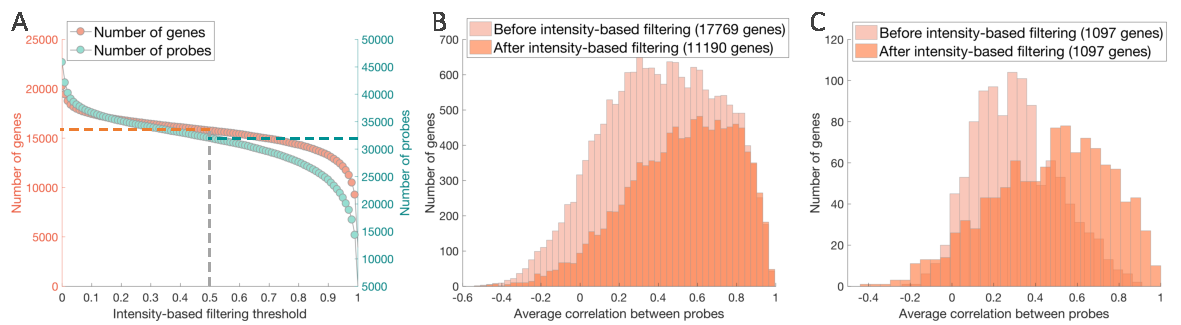
\includegraphics[width=1\textwidth]{Chapter4/Ch4Fig3.pdf}
\caption{\textbf{Intensity-based filtering (IBF) is consistent with an increase in a real expression signal, increasing the average inter-probe correlation for individual genes.} (A) The number of probes and genes as a function of filtering threshold: $x$ axis – the minimum proportion of samples with expression values exceeding the background; $y$ axis – the number of probes and genes retained. Dotted lines correspond to the number of probes and genes retained after 50\% filtering threshold was applied.
(B) Average correlation between expression values measured using all available probes for the same gene: light orange -- original set of \num{17769} genes with more than 1 probe; dark orange – \num{11190} gene set after intensity-based filtering with more than one probe, where probes for which 50\% of samples do not survive IBF are removed.
(C) Distributions of average correlations between expression values measured using all available probes for the same gene that demonstrated any change after IBF (1097 genes, or $\sim$10\% genes with multiple probes). }

\label{fig:Ch4Fig3}
\end{figure}

\subsection{Step 3. Probe selection}

Multiple probes can be used to measure the expression level of a single gene at different exons (segments of RNA molecules that code for a protein or peptide sequence), which can increase the reliability of the measurement. After performing re-annotation and IBF, 71\% genes in the AHBA were measured with at least two probes (compared to 93\% in the original data). One might expect that probes measuring the expression of the same gene should show consistent expression patterns, but this is not always the case. Differences between probes measuring the same gene can arise from different sources, including errors in probe sequences immobilised on the array during manufacturing; errors in mapping probe sequences to mRNA transcripts; inaccuracies in probe-to-gene annotations; probe-specific differences in hybridization specificity; and multiple splice variants of specific genes [for further details, see \citet{Liu2010}, and \citep{Jaksik2015}]. We find that, even after IBF, the correlation between probes measuring the expression levels of the same gene is $\rho < 0.3$ for more than 20\% of genes (Figure \ref{fig:Ch4Fig3}B). Investigators have used different strategies to derive a representative measure of gene expression some of which are summarized in Table \ref{Table2}.

\begin{table}[h!]
\caption{Methods used for deriving an estimate of gene expression in cases where multiple probes are available for the same gene.}
\label{Table2}
\resizebox{\textwidth}{!}{%
\begin{tabular}{ll}
\hline
\multicolumn{1}{c}{\textbf{Method}} & \multicolumn{1}{c}{\textbf{Description}} \\ \hline
Mean & \begin{tabular}[c]{@{}l@{}}
Calculate the mean of all available probes for a gene. \citet{Tan2013,French2015,Eising2016} \\ \citet{Krienen2016,Vertes2016b,Whitaker2016a,Negi2017,McColgan2018} \end{tabular} \\ \hline
Max intensity & \begin{tabular}[c]{@{}l@{}}
Select probe with the highest expression level. \citet{Romero-Garcia2018} \end{tabular} \\ \hline
Variance & \begin{tabular}[c]{@{}l@{}}
Select the probe with the highest variance across brain regions. \citet{Negi2017} \end{tabular} \\ \hline
PC & \begin{tabular}[c]{@{}l@{}}
Select the probe with the highest loading onto the first principal component of probes. \citet{Parkes2017} \end{tabular} \\ \hline
Differential stability (DS) & \begin{tabular}[c]{@{}l@{}}
Select the probe with most consistent pattern of regional variations cross the six donor \\ brains, as quantified using a measure called Differential Stability (DS). \citet{Hawrylycz2015,Kirsch2016a} \end{tabular} \\ \hline
Correlation variance/intensity & \begin{tabular}[c]{@{}l@{}}
Select the probe with the highest average correlation to other probes$^{a}$ for \textgreater{}2 probes; select the probe with maximum \\ variance (correlation variance) or maximum intensity (correlation intensity) when only 2 probes available. \\ \citet{Hawrylycz2012,Hawrylycz2015,Myers2015a,Burt2018,Forest2017,Anderson2018} \end{tabular} \\ \hline
Sequence mismatches & \begin{tabular}[c]{@{}l@{}}
Select the probe with fewest sequence mismatches, or the probe with highest standard deviation if \textgreater 1 probe have \\ the same number of mismatches$^{b}$. \citet{Richiardi2015} \end{tabular} \\ \hline
\end{tabular}}
\begin{tablenotes}
     \item[1] $^{a}$ This measure is implemented in the R function ‘collapseRows’ from WGCNA package \citep{Miller2011}. Here we used a custom implementation of this function that was applied for samples within each brain separately in order to account for potential inter-individual differences in gene expression (discussed in step 5).
     \item[2] $^{b}$ Sequence mismatch is defined by Re-annotator software as the difference between probe sequence and the reference genome sequencing data. Considering that $\sim93\%$ probes were re-annotated without any mismatches, the overwhelming majority of probes will be chosen applying the highest standard deviation criteria and resemble maximum variance selection approach. Therefore, this probe selection criteria was not implemented separately and is not presented in the probe selection comparison plots.
   \end{tablenotes}
\end{table}

To evaluate how the gene expression measures vary under different probe selection methods, we estimated, a single summary measure of expression for each gene indexed by multiple probes, according to one of the methods listed in Table \ref{Table2}. We also evaluated a few other methods beyond those used in the published literature, such as selecting the probe with maximum coefficient of variation across samples (CV), or the probe with the highest proportion of samples with expression levels exceeding background noise (signal proportion). In addition, we included random probe selection (averaged over 100 repeats) for comparison. We then took the expression vector of each gene across tissue samples and computed the Spearman rank correlation coefficients  between these vectors estimated for each possible pair of methods.

Figure \ref{fig:Ch4Fig4}A shows the average correlation between expression measures selected using different criteria, averaged across \num{17769} genes assayed by multiple probes. Since most studies using the AHBA do not report using IBF, we show results for unfiltered data (similar results were obtained using IBF, see Figure \ref{fig:Ch4Sfig1}). The average correlation coefficients between probe selection methods range between $0.5 < \bar{\rho} < 0.98$, indicating that the probe selection method can have a major impact on expression estimates. The method of summarizing the expression measures for a gene as the mean across all available probes is the most highly correlated, on average, to all the other methods. Variance-related methods [coefficient of variation, maximum variance, correlation-variance and highest loading on first PC of non-normalized data \citep{Parkes2017}] are similar to each other, but different to other methods. Consistency (DS) and intensity (max intensity, signal proportion and correlation-intensity) related methods, on the other hand, are more correlated with each other. Notably, the correlations between gene expression measures selected based on the highest CV compared to the consistency/intensity-related criteria are much lower than resulting from the random probe selection strategy, indicating that these methods favour dissimilar properties of expression measures for probe selection. A more detailed discussion of these results is presented in \ref{app:AppendixCh4_3}.

\begin{figure}[h!]
  \centering
    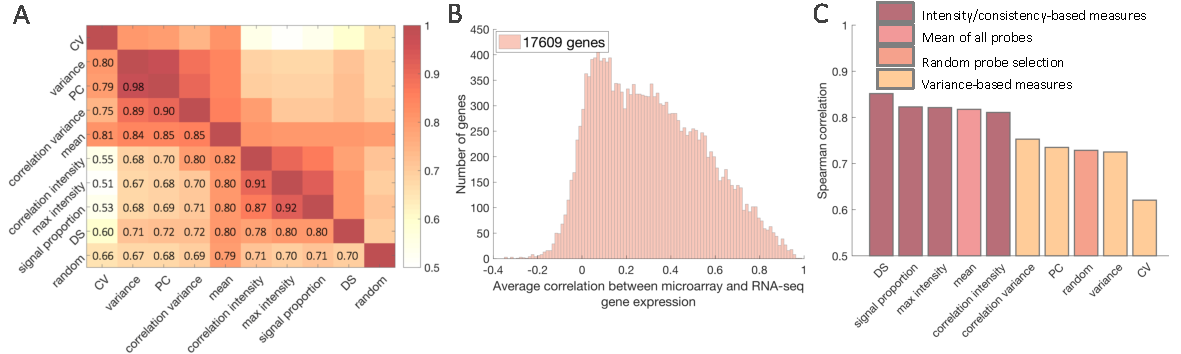
\includegraphics[width=1\textwidth]{Chapter4/Ch4Fig4.pdf}
\caption{\textbf{The probe selection method can have a large effect on resulting gene expression estimates.}
(A) Mean Spearman correlation coefficient of expression levels across \num{17769} genes with multiple probe annotations, using a range of different probe selection methods: CV, variance, PC, signal proportion, DS, correlation variance, correlation intensity, mean (see Table \ref{Table2}) or selecting a representative probe at random (correlation values averaged over 100 runs).
(B) The distribution of Spearman correlation values between microarray and RNA-seq expression data for genes that are present in both datasets. When multiple probes for a gene are available, the maximum correlation value between probes was selected.
(C) Average correlation between probes selected using RNA-seq (by selecting the probe that is most correlated with the RNA-seq data) and other methods (ordered by decreasing values), based on \num{10221} genes that: (i) had more than one probe available; (ii) were present in both microarray and RNA-seq datasets; (iii) were correlated to RNA-seq ($\rho > 0.2$, Spearman's rank correlation) to ensure that RNA-seq based probe selection provides a meaningful estimate in regards to the microarray data.}
\label{fig:Ch4Fig4}
\end{figure}

The lack of a gold standard makes it difficult to choose between different probe selection options. One strategy is to use RNA-seq data as an external reference \citep{Miller2014a}. Comparing expression values for matching structures in each of the two brains allows us to select probes that correlate most strongly with RNA-seq, providing an additional quality control measure to cross-validate probe selection.

Considering that \num{17609} of the \num{20232} genes in the microarray data have RNA-seq measures, we first aimed to evaluate whether excluding the $\sim13\%$ of genes that do not overlap between the datasets would eliminate brain-relevant genes. We verified this using over-representation analysis ORA, which is designed to identify statistically over-represented gene categories \citep{Gillis2010}: the genes removed are not enriched in brain-specific functions but rather are related to generic processes such as septin assembly and organization, as well as the negative regulation of RNA splicing (see supplementary file enrichmentExpression.csv for results and \ref{app:AppendixCh4_2} for more details).

We then examined the correlations between microarray and RNA-seq expression measures in the \num{17609} genes that overlap between both RNA-seq and microarray datasets across 112 brain regions, as shown in Figure \ref{fig:Ch4Fig4}B. Most correlations are low, with 52\% of genes exhibiting a correlation $\rho < 0.3$ and only 23\% genes exhibiting a correlation $\rho > 0.5$. This divergence between RNA-seq and microarray is likely to be caused by inaccuracies in the microarray measurements. Using GSR analysis \citep{Gillis2010}, we find that genes with higher correlations between microarray and RNA-seq are related to neuronal connectivity and communication related processes with categories such as ‘transmission of nerve impulse’, ’ensheathment of neurons’, ‘myelination’ and ‘glial cell development’ demonstrating the strongest enrichment (see supplementary file enrichmentExpression.csv for results and \ref{app:AppendixCh4_2} text for more details). This analysis suggests that RNA-seq data can be used as a reference to select brain-relevant and reliably measured genes.

Figure \ref{fig:Ch4Fig4}C shows that, compared to other probe selection methods, RNA-seq demonstrates the highest similarity to intensity/consistency-based approaches ($\rho > 0.8$, Spearman's rank correlation), with DS showing the highest correlation. In contrast, variance-based methods are no more similar to the RNA-seq measures than random probe selection ($\rho < 0.75$, Spearman's rank correlation). Given that RNA-seq data is only available for a limited number of samples (with only 87\% of genes being represented), and the data come from only two of the six donor brains in the AHBA, Figure \ref{fig:Ch4Fig4}C indicates that DS may be a reasonable alternative method for probe selection that can be generalized to the full AHBA.

\subsection{Step 4. Assigning samples to brain regions}

The AHBA provides gene expression data for multiple spatially localized tissue samples (Figure \ref{fig:Ch4Fig1}). When relating such data to macroscopic IDPs, it is necessary to generate some mapping between the spatial location of each tissue sample and the particular spatial unit of analysis (e.g., voxel, brain region) used to construct the IDP. This mapping is facilitated by the AHBA including an MNI coordinate (and voxel coordinate) for each tissue sample, and MRI data acquired for each individual brain contained in the AHBA. Each tissue sample is also associated with an anatomical structure ID, which can be related to corresponding higher order structures using the Allen Institute anatomical ontology, allowing brain structures to be identified at different resolution scales.

Existing studies have used several approaches to map tissue samples to regions-of-interest (ROIs) in imaging data.
One strategy has been to match samples to structures based on the name of a given anatomical sample. The simplest approach is to use the anatomical structure names provided by the AHBA [see \citet{AHBAdoc,Tan2013,Myers2015a,Chen2016,Kirsch2016a,Hecker2017,Lee2017a,Negi2017}], but these regions do not directly correspond to brain parcellations typically used in imaging analyses, so precise alignment with imaging data can be difficult. An alternative approach is to use the MNI (or voxel) coordinates of each sample \citep{Goyal2014,Cioli2014b,French2015,Richiardi2015,Komorowski2016,Krienen2016,Rizzo2016,Burt2018,Parkes2017,Romme2017,Shin2017,Anderson2018,Romero-Garcia2018}.
It is possible to either assign samples to brain regions in a single parcellation defined in MNI space \citep{Krienen2016,Keo2017,Parkes2017,Romme2017}, or to assign samples to regions based on parcellations of each individual AHBA brain \citep{Romero-Garcia2018}. The former approach is simpler, but a characteristic of the AHBA is that the MNI coordinates provided for each tissue sample are based on spatial normalizations that were tailored to each individual brain. Specifically, two of the AHBA brains were scanned \textit{in cranio} and normalized to MNI space via a linear transformation, whereas the other four were acquired \textit{ex cranio} and normalized using an affine followed by a non-linear transformation [for details see \citep{AHBAdoc}] with the deformation fields also being smoothed to facilitate matching the images to Nissl stains. These differences across brains will influence the accuracy of the normalization across the six brains, which is compounded by differences in tissue distortion that occurred during sample handling and processing.

To overcome these issues, a parcellation scheme can be applied to each individual donor brain. This method can more accurately account for individual differences in anatomy but is contingent on being able to generate appropriate transformations between native and MNI space for an accurate parcellation. For cortex, the accuracy of the parcellation can be greatly enhanced by parcellating and normalizing the surface while the parcellation of non-cortical areas requires volumetric normalization. In our own work, we have been able to segment the cortical surfaces of the six AHBA brains with reasonable accuracy (assessed by visual inspection), and we supply four different volumetric parcellations mapped at different resolutions to each brain using FreeSurfer: the Desikan-Killany \citep{Desikan2006}, comprising $34$ nodes per hemisphere, the group-level HCPMMP1 \citep{Glasser2016} comprising $180$ nodes per hemisphere, and two random parcellations comprising $100$ and $250$ nodes per hemisphere, respectively.

Once a particular parcellation has been generated, tissue samples should be assigned to the nearest region of the parcellation. In this assignment, a threshold can also be applied, to avoid assigning samples beyond a certain distance. The distance between sample and region is commonly estimated as the Euclidean distance in 3D space. This sample-region distance has been computed in different ways, including representing a region in space by its centroid coordinate \citep{Vertes2016b,Whitaker2016a,McColgan2018}, or taking the minimum distance between the sample and any voxel in the region \citep{French2015,Parkes2017,Romme2017}. The latter approach is more accurate, given that regions in any given parcellation vary in size and folded geometry (e.g., Figure \ref{fig:Ch4Fig5}A).

\begin{figure}[h!]
  \centering
    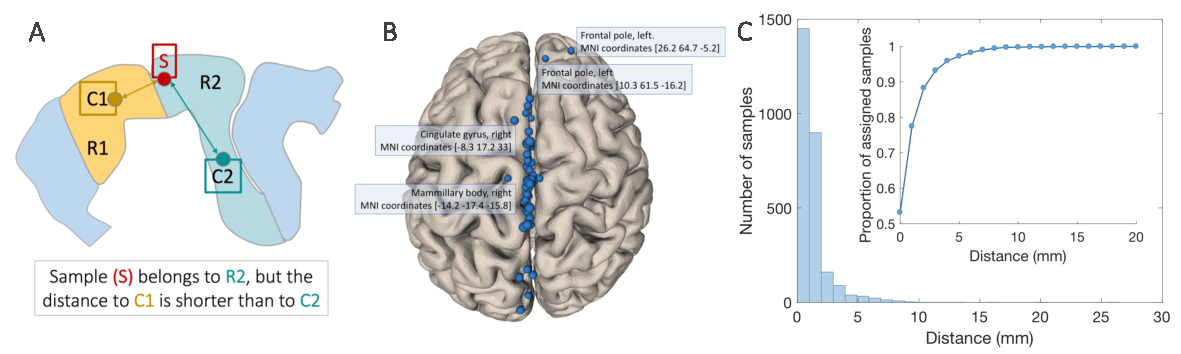
\includegraphics[width=1\textwidth]{Chapter4/Ch4Fig5.pdf}
\caption{\textbf{Methods for assigning localized tissue samples to matching regions in a brain parcellation are sensitive to the metric used to define sample-region distances, the distance threshold used, and the use of anatomical annotations on individual samples.}
(A) Schematic representation of sample assignment when a sample is assigned to the closest ROI centroid. A given sample belongs to region R2 but is closer to the centroid (C1) of region R1 than the centroid (C2) of R2, resulting in an erroneous assignment.
(B) Schematic representation of samples that were assigned to a hemisphere that differed from the annotations provided with their MNI coordinates.
(C) Sample assignment using distance thresholds: the number of samples across all six brains within a given distance from a parcellation region. Insert shows the proportion of assigned samples as a function of distance threshold. At a 2 mm distance threshold, $\sim$90\%  of tissue samples can be matched to a region in the parcellation. }
\label{fig:Ch4Fig5}
\end{figure}

In this process of assigning samples to regions, errors can occur if the mapping is not done separately for (i) broad anatomical division (cortex, subcortex, cerebellum and so on); and (ii) left and right hemispheres. That is, cortical samples listed as coming from the left hemisphere in the AHBA ontology should only be mapped to left cortical voxels (as samples were taken from annatomically known positions in the brain), right subcortical or cerebellar samples to right subcortical/cerebellar voxels and so on.

In our own experience, we have observed that subcortical samples (as indicated by AHBA ontology) can be mapped to cortical regions of the parcellation as a cortical voxel may be closer (or visa versa). Similarly, if no separation between hemispheres is performed, 58 out of \num{2748} cortical and subcortical samples are assigned to an incorrect side of the brain when using the Desikan-Killany \citep{Desikan2006} parcellation (Figure \ref{fig:Ch4Fig5}B). While the majority of those samples are very close to the midline, several are clearly incorrectly mapped to the stereotaxic space, such as two samples in the frontal pole, which are assigned to the left side of the brain according to the AHBA annotations but have a positive MNI $x$-coordinate. The same is true for some samples from the mammillary body and cingulate gyrus, which are labelled as coming from the right hemisphere but have negative MNI $x$-coordinates (Figure \ref{fig:Ch4Fig5}B). To avoid potential mistakes, samples with mismatching assignments should be excluded. In addition, the AHBA ontology classifies hippocampus as a part of the cerebral cortex while most neuroimaging tools do not. Given the differences in gene expression between the neocortex and allocortex, including hippocampal samples when integrating information from the cortical sheet may give misleading results.

A second consideration is to set a distance threshold for assigning samples to regions, to ensure that samples further than a given threshold away from the parcellation will not be assigned \citep{Romero-Garcia2018}. As shown in Figure \ref{fig:Ch4Fig5}C, only around 50\% of samples are directly mapped to a parcellation when using the Desikan-Killany \citep{Desikan2006} parcellation (i.e., their coordinates correspond to a voxel inside the parcellation). Increasing the distance threshold will allow some tolerance for small errors in spatial normalization. For example, \citet{Romero-Garcia2018} implemented distance-constrained sample assignment by extending the parcellation into the white matter in order to include those cortical samples that have not been directly mapped to the parcellation. Figure \ref{fig:Ch4Fig5}C shows that assigning samples that are up to 2 mm away from any voxel in the parcellation increases the proportion of assigned samples to almost 90\%, with additional increases in the distance threshold yielding only minor gains in the number of assigned samples. Therefore, we use a 2 mm distance threshold in our analyses.

An important consideration regarding sample assignment arises from the fact that only two out of six brains were sampled from both hemispheres and four brains have samples collected only in the left. This sparse sampling should be carefully considered when combining data across donors. Restricting analyses to the left hemisphere will minimize variability across regions (and hemispheres) in terms of the number of samples available. However, if a whole-brain analysis is desired, such variability should be carefully studied to ensure that it does not impact one’s findings. In the \ref{app:AppendixCh4_4}, we provide information on the number of samples assigned to four different parcellations. One way to deal with limited anatomical coverage in the AHBA is to infer missing expression values based on some model of the data. For example, \citet{Gryglewski2018} built a Gaussian process regression model using a weighted linear combination of the nearest samples to infer the missing expression value at a particular location. Validation of model predictions in new data would support its use in extending the coverage of the current AHBA.

\subsection*{Step 5. Six brains, one atlas: accounting for individual variability}

The AHBA is often used to represent a general transcriptomic profile of the adult human brain. However, it is comprised of data taken from people aged 24 to 57 years, of different ethnicities, sexes, medical histories, causes of death, and post-mortem intervals (Table \ref{Table3}). Many of these factors can impact gene expression \citep{Fraser2005,Berchtold2008,Kumar2013,Trabzuni2013}. One way to address this brain-specific variance is to conduct analyses separately in each brain. However, spatial coverage of different brain areas in the AHBA varies from person to person. Therefore, collapsing samples from all brains to derive a single atlas with maximum spatial coverage. In this case, an appropriate correction for donor-specific transcriptomic patterns is required.


\begin{table}[h!]
\caption{Information about the six adult donors in AHBA.}
\label{Table3}
\resizebox{\textwidth}{!}{%
\begin{tabular}{llllll}
\hline
\multicolumn{1}{c}{\textbf{Donor}} & \multicolumn{1}{c}{\textbf{Age}} & \multicolumn{1}{c}{\textbf{Sex}} & \multicolumn{1}{c}{\textbf{Ethnicity}} & \multicolumn{1}{c}{\textbf{Medical conditions}} & \multicolumn{1}{c}{\textbf{Post-mortem interval$^{a}$}} \\ \hline
H0351\_2001$^{b}$ & 24  & Male   & \makecell{African \\ American} & \begin{tabular}[c]{@{}l@{}}History of asthma \end{tabular} & 23 hours \\ \hline
H0351\_2002$^{b}$ & 39  & Male   & \makecell{African \\American} & \begin{tabular}[c]{@{}l@{}}Possible small pituitary adenoma; \\single neurofibrillary tangle in entorhinal cortex \end{tabular}                                                                                                      & 10 hours \\ \hline
H0351\_1009 & 57  & Male   & Caucasian        & \begin{tabular}[c]{@{}l@{}}History of atherosclerotic cardiovascular disease \end{tabular}                                                                                                                                        & 25.5 hours            \\
\hline
H0351\_1012 & 31  & Male   & Caucasian        & \begin{tabular}[c]{@{}l@{}}Sudden cardiac arrest; benign spindle cell \\ proliferation and dystrophic calcification \\ in temporal horn of lateral ventricle \end{tabular}                                                               & 17.5 hours            \\
\hline
H0351\_1015 & 49  & Female & Hispanic         & \begin{tabular}[c]{@{}l@{}}Splenectomy, hypothyroidism treated with Levothroid;\\ modest numbers of hemosiderin laden macrophages \\ noted in Virchow-Robin spaces in parietal and occipital \\ lobes, mild arteriosclerosis \end{tabular}
& 30 hours              \\
\hline
H0351\_1016 & 55  & Male   & Caucasian        & \begin{tabular}[c]{@{}l@{}}Coronary artery atherosclerosis, prescriptions \\ for clotting and high cholesterol                                                                                                         \end{tabular} & 18 hours              \\
\hline
\end{tabular}}
\begin{tablenotes}
     \item[1] $^{a}$ Post-mortem interval is defined as the time period from the time of death to the time the tissue is frozen.
     \item[1] $^{b}$ These donors have tissue samples collected across both left and right hemispheres while all the other donors have samples only from within the left hemisphere.
   \end{tablenotes}
\end{table}

The Allen Institute applied a range of data normalization procedures to remove batch effects and artefactual inter-individual differences. Nonetheless, residual inter-individual differences remain (Figure \ref{fig:Ch4Fig6}A). While a number of studies account for the additional inter-individual differences between donor brains through subject-specific normalization prior to aggregation \citep{Richiardi2015,Whitaker2016a,Vertes2016b,Negi2017,Liu2017,Romero-Garcia2018,Burt2018,McColgan2018}, some perform normalization after aggregating across subjects \citep{Parkes2017} or do not explicitly specify inter-subject normalisation \citep{Veronese2016}. Here we investigated whether intrinsic inter-individual differences in gene expression are able to discriminate individual donor brains by projecting all tissue samples from all six brains into a two-dimensional transcriptional principal components space. Figure \ref{fig:Ch4Fig6}A plots loadings of each cortical tissue sample on the first two principal components of gene expression for all six donors (for the whole brain see Figure \ref{fig:Ch4Sfig5}). This unsupervised projection of samples into gene expression space captures the latent dimensions of variance between all samples and broadly separates the six donors (regardless of where a tissue is located in the brain), indicating that each donor has a distinctive gene expression profile. In other words, while the data normalization procedures applied by the Allen Institute prior to data release removed batch effects and artefactual inter-individual differences, a considerable degree of intrinsic donor-specific variance remains and must be accounted for in order to perform valid data aggregation.

\begin{figure}[h!]
  \centering
    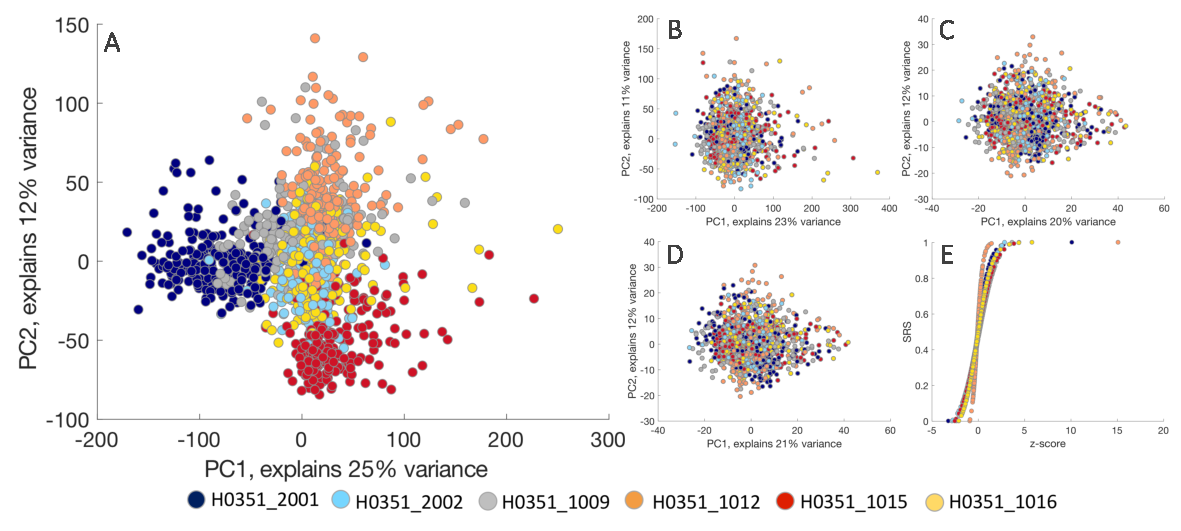
\includegraphics[width=1\textwidth]{Chapter4/Ch4Fig6.pdf}
\caption{\textbf{Appropriate normalization can remove donor-specific variability in gene expression.}
(A) Non-normalized gene expression data in principal component (PC) space. Data from different donors are represented in different colours. Samples from different subjects occupy different parts of the low-dimensional gene expression space. Panels B,C represent gene expression data in principal component space normalized separately for each subject using $z$-scores
(B) or the scaled robust sigmoid (SRS) transform 
(C). Panel D shows gene expression data in principal component space after applying \textit{limma} batch effect removal \citep{Ritchie2015} on cross-subject aggregated data, followed by SRS normalization. After normalization (B,C,D), samples no longer segregate by donor. 
(E) Correlations between normalized expression values ($z$-score \textit{vs} SRS) for the ZZZ3 gene (chosen for visualization purposes).
Each dot represents a normalized expression value for ZZZ3 gene across samples, and different colours correspond to different subjects. The $z$-score normalization results in extreme values being assigned to outliers, therefore producing different scales for subjects and complicating direct comparison of values.
This example demonstrates how outliers in the data can affect the scaling for different subjects: using $z$-score normalization results in different scales for different subjects with normalized values ranging from approximately $-5$ to $5$ for four out of six subjects, whereas subjects H0351\_1012 (orange) and H0351\_2001 (dark blue) have a much wider range. In comparison, SRS produces normalized expression values on the same scale for each subject without being affected by outliers.
Representations in principal component space are based on \num{10028} genes, with representative probes chosen based on correlation to RNA-seq data. }
\label{fig:Ch4Fig6}
\end{figure}

One approach for addressing donor-specific effects is to perform a leave-one-out analysis, where the analysis is repeated six times, excluding one of the brains at each iteration  \citep{Parkes2017,McColgan2018}. Such an approach can rule out the undue influence of any single brain, provided that the results are consistent across iterations. A more direct way of eliminating the inter-individual differences in expression measures is to normalize the gene expression data separately for each subject \citep{Richiardi2015,Whitaker2016a,Vertes2016b,Rizzo2016,Liu2017,Negi2017,Burt2018,McColgan2018,Romero-Garcia2018a}. With this approach, each gene’s expression values are normalized across regions separately for each donor in order to reflect the relative expression of each gene across regions, within a given brain (Figure \ref{fig:Ch4Fig6}B-D). A desirable normalization procedure should offer robustness to outlying values and quantify expression on the same scale across donors to enable direct comparison. Most studies using AHBA have used $z$-score normalization \citep{Rizzo2016,Whitaker2016a,Vertes2016b,Negi2017,Romero-Garcia2018a},

\begin{equation}
    \label{eqn:eq1}
    x_\mathrm{norm} = \frac{x_\mathrm{\textit{i}}-\overline{x}}{\sigma},
\end{equation}
where $\overline{x}$ represents the mean, $\sigma$ represents the standard deviation and $x_\mathrm{\textit{i}}$ -- the expression value of a gene in a single sample. The estimates of $\overline{x}$ and $\sigma$ are appropriate for symmetric distributions, whereas gene expression distributions across brain samples are often non-symmetric, and can contain outliers, which can bias these summary statistics. Figure \ref{fig:Ch4Fig6}E demonstrates the sensitivity of $z$-score normalization to the outlying values.
A variety of outlier-robust normalizations exist such as Hampel hyperbolic tangent transformation, however here we focus on a variant of a normalization method used by \citet{Fulcher2016}, the scaled robust sigmoid (SRS) normalization \citep{Fulcher2013}. This approach normalizes gene expression values based on an outlier-robust sigmoid function,

\begin{equation}
    \label{eqn:eq2}
    x_\mathrm{y} = \frac{1}{1+\mathrm{exp}({\frac{-(x_\mathrm{\textit{i}}-\left\langle x \right\rangle)}{\mathrm{IQR}/1.35}})},
\end{equation}
where $\left\langle x \right\rangle$ represents the median and $\mathrm{IQR}$ represents the interquantile range, before rescaling normalized values to a unit interval,

\begin{equation}
    \label{eqn:eq3}
    x_\mathrm{norm} = \frac{x_\mathrm{y}-\mathrm{min(x)}}{\mathrm{max(x)}-\mathrm{min(x)}}.
\end{equation}

This normalization is robust to outliers and ensures equivalent scaling of expression values for each person. Figures \ref{fig:Ch4Fig6}C and E show the effectiveness of SRS in dealing with outliers and scaling. Other strategies for removing donor-specific effects involve using linear models applied to cross-donor combined data. For example, donor-specific effects can be treated as an additional batch effect and removed via linear modelling using the R/Bioconductor software package \textit{limma} \citep{Ritchie2015}. While this approach removes inter-individual differences in gene expression, the linear model is sensitive to outliers. This correction in turn can be followed by SRS normalization to minimize the influence of outliers (Figure \ref{fig:Ch4Fig6}D).

To account for potential between-sample differences in gene expression, \citet{Burt2018} introduced within-sample normalization across genes before subject-specific normalization across samples (see Figure \ref{fig:Ch4Sfig6}). Indeed, some samples can show a markedly different expression profile (extremely low or high values across all genes) from other samples in close spatial proximity, potentially due to measurement artefacts. The influence of these artefacts can be minimized by applying within-sample cross-gene normalization to quantify relative expression levels within a given sample, before normalizing across samples. To quantify the effect of the initial within-sample normalization, we calculated the correlations between expression values across genes and samples in two cases: i) when only cross-sample normalization for each gene was applied; ii) when both cross-gene normalization within sample as well as cross-sample normalization for each gene were applied. While the correlation values were relatively high ($\mathrm{median_\mathrm{sample}}(r) =  0.97$, $\mathrm{IQR} = 0.04$; $\mathrm{median_\mathrm{gene}}(r) = 0.86$, $\mathrm{IQR} = 0.1$), based on visual inspection, the initial within sample normalization was beneficial in reducing potential measurement artefacts in the data.

One additional consideration is that the spatial distribution of tissue samples across individual brains in the AHBA is not uniform. As such, different brains can contribute a different number of samples to any given brain region (Figure \ref{fig:Ch4Fig1} and Figure \ref{fig:Ch4Sfig7}). In light of this variability, we have two choices: we can either average all samples falling within a region, meaning that the average may be driven by a subset of individuals who have more samples localized to that region, or we can average at the level of each individual donor brain before aggregating across people (Figure \ref{fig:Ch4Sfig7}). The latter approach ensures that each donor makes an equal contribution to the mean, provided that all genes are normalized to the same scale. While the choice of inter-subject averaging does not significantly impact whole-brain analyses, it might have a more pronounced effect if the analysis is focused on a particular region where samples are not evenly distributed across donors (for a more detailed explanation see Figure \ref{fig:Ch4Sfig7}).

\subsection{Step 6. Gene filtering}

The AHBA consists of more than \num{20000} unique genes, of which only a fraction is expected to show consistent regional variations in expression across the brain. Many analyses interested in transcriptomic signatures of IDPs will be primarily interested in these brain-specific genes. Various methods for pre-selecting genes of interest have been adopted, including selecting: (i) disease-specific genes \citep{Rittman2016,Romme2017,Yokoyama2017a}, (ii) genes related to a priori hypotheses \citep{Goyal2014,Komorowski2016,Krienen2016,Acevedo-Triana2017}, (iii) genes that are expressed consistently across all six AHBA brains, as quantified using the DS measure \citep{Hawrylycz2015}, or (iv) demonstrate consistent expression between different gene expression datasets \citep{Shin2017}. Genes with high DS values demonstrate consistent patterns of regional variation in expression across the six AHBA subjects, and have been shown to be enriched for brain-related biological functions \citep{Hawrylycz2015}. Filtering based on DS thus offers a more targeted approach for investigating relationships between IDPs and gene expression compared to whole-genome analysis.

The selection of disease-specific genes is traditionally based on previous GWAS studies \citep{Satake2009,Simon-Sanchez2009,Hoglinger2011,Ferrari2014,Ripke2014a,Kouri2015}, while gene selection based on an \textit{a priori} hypothesis can depend on other factors such as a specific involvement in clinical disorders \citep{Komorowski2016,Acevedo-Triana2017}. One particular set of 19 genes demonstrating a selective enrichment in the upper layers of the human cortex compared to mouse [Human Supragranular Enriched (HSE) genes] has been extensively investigated and was found to be related to measures of functional connectivity \citep{Krienen2016} and brain network topology \citep{Vertes2016b,Romero-Garcia2018}.

\subsection{Step 7. Accounting for spatial effects}

The application of steps 1 to 6 results in a processed region $\times$ gene matrix of transcription level values, which can be used for further analyses. Typically, the data are linked to IDPs at either the regional level, or at the level of pairs of regions [i.e., patterns of correlated gene expression (CGE) between pairs of brain regions are related to pair-wise measures of structural or functional connectivity between those regions \citep{Fornito2019}]. In both cases, we seek to understand how spatial variations in gene expression or CGE relate to spatial variations in the IDP. One complicating factor is that cortical regions that are located in close proximity are more likely to share similar gene expression patterns \citep{Richiardi2015,Krienen2016,Vertes2016b,Pantazatos2017,Richiardi2017}. A similar spatial autocorrelation of gene expression has been reported in the mouse brain \citep{Fulcher2016} and in the head of the nematode \textit{C.elegans} \citep{Arnatkeviciute2018}.

In some respects, this distance-dependence of gene expression is an interesting and physiologically meaningful trend that warrants further investigation [for a review, see \citep{Fornito2019}]. However, if an IDP varies across the brain in a manner that reproduces a spatial gradient in gene expression, any apparent association between the IDP and gene expression measures may be driven by low-order spatial effects. Depending on the research question, especially when a direct relationship between an IDP and gene expression is evaluated, it is important to confirm that the identified association is stronger than what would be expected based on the spatial autocorrelation properties of gene expression (if such an effect is claimed). For example, a researcher may wish to show that CGE is higher between nodes belonging to the same brain functional network. As spatially adjacent regions are more likely to belong to the same functional system, such an effect may simply be driven by their separation distance rather than their functional identity. If one wishes to conclude that elevated CGE is related specifically to functional network affiliation, then the influence of spatial separation on CGE must be addressed. Indeed, this has been a topic of some debate in the literature \citep{Richiardi2015,Pantazatos2017,Richiardi2017}.

A critical first step in understanding spatial biases in gene expression is to define distances between brain regions. These distances can be estimated by (i) calculating the Euclidean distance between regions; (ii) estimating the shortest distance within the grey matter volume; or (iii) estimating the shortest distance on the cortical surface (Figure \ref{fig:Ch4Fig7}), see \ref{app:AppendixCh4_5} for more details. The Euclidean distance is the simplest method, but it approximates distances as straight lines that do not respect cortical geometry. Calculating distances within the grey matter volume or on the cortical surface present a more biologically valid approach, as distances are constrained by cortical geometry. A comparison of these methods, shown in Figure \ref{fig:Ch4Fig7}D, demonstrates that evaluating the Euclidean distance results in shorter distances, on average, compared to other methods, while anatomically constrained volume and surface-based approaches yield similar distance estimates in cortex. Note that the Euclidean approach is easier to generalize for measuring distances to subcortex.

\begin{figure}[h!]
  \centering
    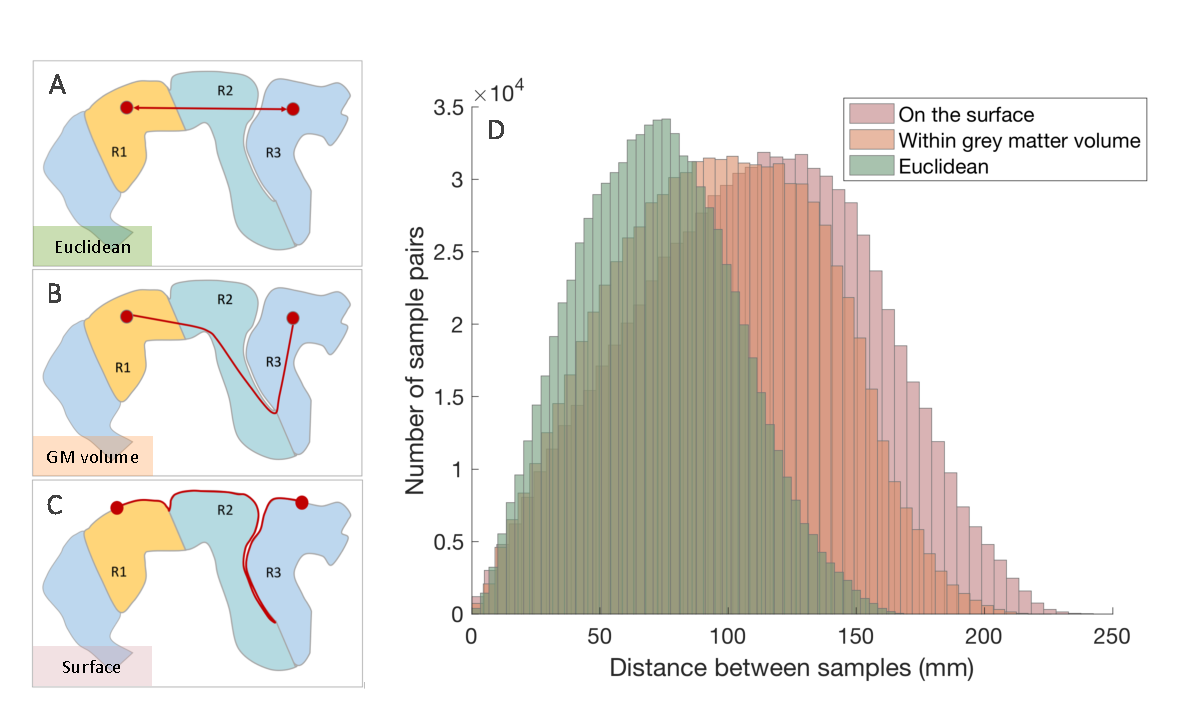
\includegraphics[width=1\textwidth]{Chapter4/Ch4Fig7.pdf}
\caption{\textbf{Distances between samples can be defined in different ways.}
Schematic representation of different approaches to calculate the distances between samples.
(A) Euclidean distance, defined as the shortest distance between two points.
(B) Distance within grey matter defined as the shortest distance within the grey matter volume. This measure is implemented by representing each voxel in the cortex as a node and creating a three-dimensional network where the shortest distances between brain regions are found using Dijkstra's algorithm \citep{Dijkstra1959}. The resulting distances will approximate the distances between regions within the cortical volume.
(C) Distance on a mesh-based representation of the cortical surface, where gene expression samples are assigned to vertices in the mesh and the shortest distance is calculated as a shortest path between them. Both Euclidean and grey matter distances can be calculated using volumetric parcellation schemes, while estimating the distance on the cortical surface requires generating a surface-based cortical parcellation.
(D) Distributions for pairwise sample distances calculated using the three approaches. Euclidean distance estimates are lower compared to both distances estimated within grey matter volume and on the surface. }
\label{fig:Ch4Fig7}
\end{figure}

Spatial effects are most easily examined in the context of analyses of correlated gene expression. Such analyses focus on patterns of pair-wise or multivariate transcriptional coupling between regions, where transcriptional coupling is estimated as a correlation between regional expression profiles. Such measures of CGE can then be related to some inter-regional IDP, such as a measure of functional or structural connectivity \citep{Richiardi2015,Fulcher2016,Arnatkeviciute2018}. Figure \ref{fig:Ch4Fig8}A shows that CGE decays sharply as a function of increasing spatial distance (on the pial surface) between regions in the cortex; relationships for other distance measures are qualitatively similar (see Figure \ref{fig:Ch4Sfig8}). In line with previous findings in different species \citep{Fulcher2016,Arnatkeviciute2018}, the dependence of CGE on distance can be approximated as an exponential (Figure \ref{fig:Ch4Fig8}A) and therefore the residuals of the exponential fit could be further used in the analyses (Figure \ref{fig:Ch4Fig8}B). Extending this relationship to the whole brain, including samples from both cortex and subcortex, is complicated by a strong anti-correlation between cortical and subcortical gene expression \citep{Hawrylycz2015}. Thus, separate normalization procedures for cortical and subcortical regions and corrections for different types of region pairs can be applied (see \ref{app:AppendixCh4_6} and Figure \ref{fig:Ch4Sfig9} for more details). Note also that the dependence of CGE on distance can vary as a function of the gene set and parcellation being used (see Figure \ref{fig:Ch4Sfig10}).

\begin{figure}[h]
  \centering
    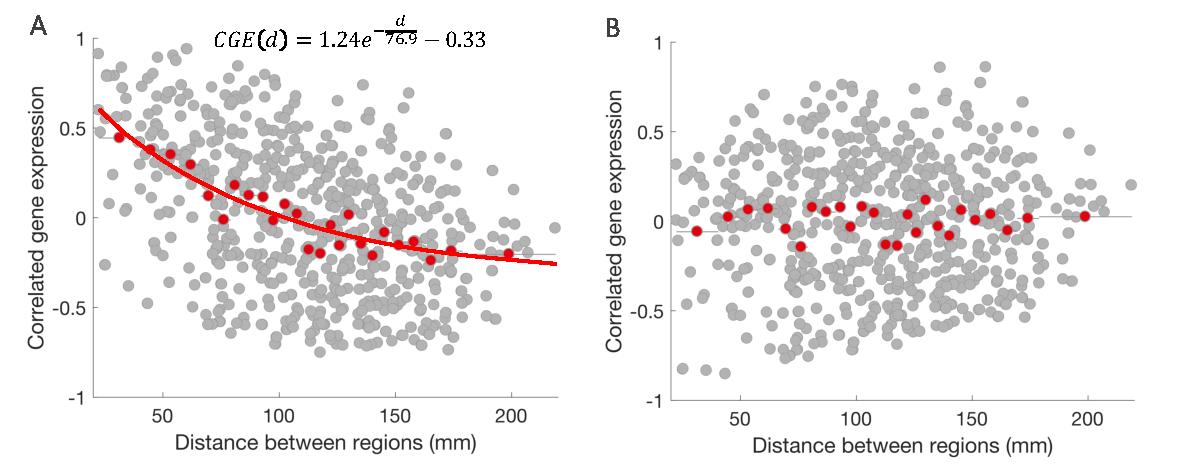
\includegraphics[width=1\textwidth]{Chapter4/Ch4Fig8.pdf}
\caption{\textbf{Characterizing the distance-dependence of gene expression data.}
(A) CGE as a function of separation distance on the cortical surface. The red line represents an exponential fit $CGE(d) = 1.24e^{-d/76.9}-0.33$.
(B) CGE residuals after removing the exponential trend. CGE between pairs of regions are represented in grey dots and red dots represent the mean value in 25 equiprobable distance bins after the correction. CGE calculated using all \num{10027} genes (after intensity-based filtering and probe selection based on correlation to RNA-seq data).}
\label{fig:Ch4Fig8}
\end{figure}

Characterizing and removing distance dependence can be relatively straightforward in analyses of CGE. Addressing spatial relationships in analyses of regional gene expression can be more challenging since distance is defined between pairs of regions, whereas a regional expression value is a property of a single region. Some promising strategies to deal with this issue involve comparing observed findings relative to an appropriate null model. One class of methods uses spatially constrained permutation of the original data. Arbitrarily-defined regions are not independent from one another, so some spatial constraints are required to account for these dependencies during permutation. As an example, a block permutation algorithm implemented by \citet{Vertes2016b} accounted for spatial relationships between regions by aggregating areas into spatially contiguous subsets (blocks) according to the Desikan-Killiany atlas, and then permuting the resulting blocks rather than individual regions. \citet{Vasa2018} introduced a spatial permutation test based on the rotation of regional coordinates in the spherical projection, such that the relative spatial relationships between regions are preserved. Matching between original and rotated coordinates, therefore, allows the regional measure to be permuted while controlling for spatial contiguity and hemispheric symmetry. \citet{Burt2018} used a spatial lagged autocorrelation model to characterise the spatial dependency between observed gene expression values. Moreover, while these approaches provide some valid options, thorough evaluation of these null models is an important avenue of future work. While distance is perhaps the most obvious influence to consider correcting in expression analyses, other factors, such as regional variations in cytoarchitecture and cell density, are also relevant considerations \citep{Barbas2015,Burt2018}. The appropriateness of different corrections should be carefully motivated by the specific research question.

\begin{table}[H]
\caption{Recommendations and practical considerations for each data processing step.}
  \centering
    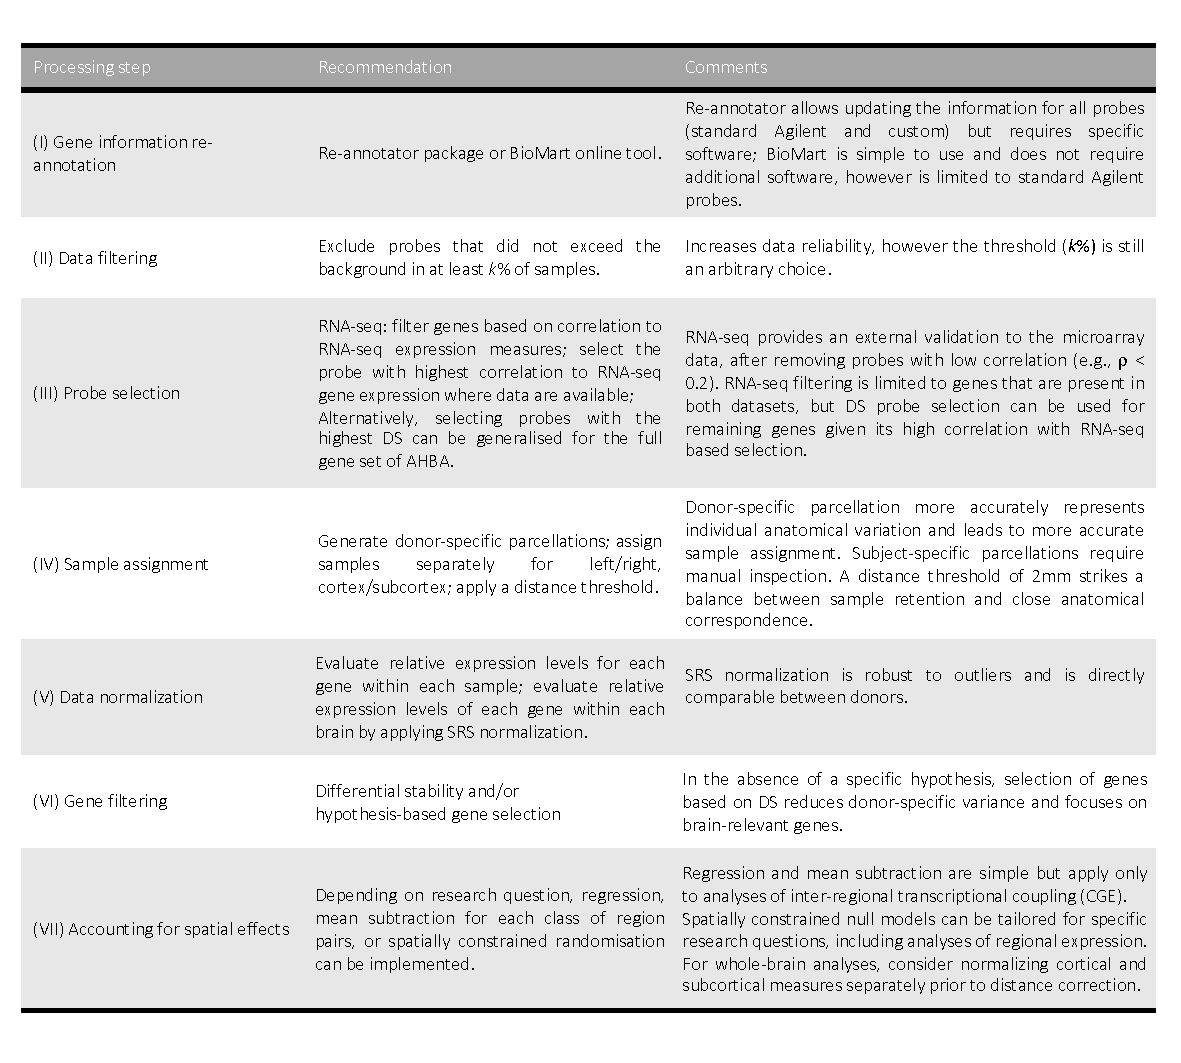
\includegraphics[width=1\textwidth]{Chapter4/Ch4Fig9.pdf}
\label{fig:Ch4Fig9}
\end{table}

\section{Conclusions}

Imaging transcriptomics provides an unprecedented opportunity to uncover the molecular basis of large-scale brain organization [for a review, see \citep{Fornito2019}]. Given the rapid development of this field and its heavy reliance on publicly available data, there is a pressing need for standardized data processing pipelines that will facilitate the comparison of findings across studies. Our analysis delineates seven core steps of a basic workflow and demonstrates how choices at each step may affect the final expression measures. While the order of some processing steps might strongly influence the data--for instance, intensity-based filtering should be done before probe selection in order to avoid selecting probes with very low intensity — the order of other steps (e.g., 3-5) may be interchangeable. We summarize some preliminary recommendations for best practice in Table \ref{fig:Ch4Fig9}.

Considerable further work is required, particularly in the development of methods for addressing spatial correlations in the data. The development of standardized workflows will be essential to ensure reproducibility, particularly as gene expression atlases become more widely available and increase in their sophistication \citep{Lein2007a,Harris2010,Miller2014}. We have focused here on the processing of expression measures and removal of inherent biases in the data. Another area requiring further work is the development of appropriate statistical methods for relating IDPs to transcriptomic measures. For example, there is considerable variability in the software packages used for enrichment analyses, each of which makes different assumptions and uses different annotations of genes to gene ontology and other categories \citep{Rhee2008}. It will be important to understand how the available choices for analyzing these data influence reproducibility. 

\section*{Acknowledgments}

We would like to thank A/Prof David Powell, Dr. Sarah Williams, and Dr. Leon French for valuable comments regarding the gene expression data processing.
  
  \clearpage
  %!TEX root = ../Thesis.tex
\chapter{Genetic markers of hub connectivity in the human brain}
\label{ch:Chapter5}
\fancyhead[R]{\textit{Chapter.} \textit{\thechapter: }\textit{Genetic markers of hub connectivity in the human brain}}

\textbf{Aurina Arnatkevi\u{c}i\={u}t\.{e}},
Stuart Oldham,
Ben D. Fulcher,
Mark Bellgrove,
Alex Fornito.
Genetic markers of hub connectivity in the human brain. \textit{This manuscript is currently in preparation}.\\

\section*{Preamble}
The ultimate goal of this thesis is to investigate genetic markers of hub connectivity across different scales. Building on the previous work in the mesoscale \citep{Fulcher2016} and microscale [\citep{Arnatkeviciute2018}, presented in Chapter 2] connectomes, we next aimed to comprehensively examine the genetic markers of hub connectivity in the human brain through combining diffusion weighted imaging, genotyping, and AHBA gene expression data. In this chapter we investigated edge-wise, connectome-wide heritability, the effects of structural DNA variation through the polygenic scores, and the transcriptional signature of hub regions. We show that connectivity between hubs is the most highly heritable, is related to polygenic liability for mental illness, and high IQ. We also show that hubs in the human brain have elevated transcriptional coupling that is predominantly driven by metabolism-related genes, mirroring previous findings in mouse \citep{Fulcher2016} and human \citep{Vertes2016b}. Together, this work establishes a link between molecular function and large-scale connectome organization and demonstrate that the genetic influences on brain network organisation converge on hubs.\\
Supplementary materials for this chapter are in Appendix \ref{appendixC}.

\newpage

\section*{Abstract}
Nervous systems characteristically possess a relatively small number of highly connected regions, called network hubs, that are also highly interconnected with each other, forming a so-called `rich club’. Rich club organization plays an important role in supporting integrated brain function and is highly conserved, having been identified in diverse species with varying biological complexity. Such conservation points to a potential role of genes in shaping hub connectivity. Here, we comprehensively investigate genetic markers of hub connectivity in the human brain, as measured using diffusion MRI, by characterising its heritability, polygenic basis, and transcriptional signature. Using connectome-wide heritability analysis of 117 MZ and 60 DZ twin pairs, we demonstrate that the integrity of connections between hubs are under the strongest genetic control compared to hub--non-hub and non-hub--non-hub connections. At the level of structural DNA variation, we demonstrate that higher polygenic liability for psychiatric disorders is associated with reduced structural integrity of hub--hub connections, whereas higher polygenic scores for IQ are related to increased hub connection strength. Using gene expression data from the Allen Human Brain Atlas (AHBA), we show that hub regions display  tightly coupled transcriptional profiles, and that this effect is driven most strongly by genes regulating energy metabolism, mirroring results in the mesoscale mouse connectome \citep{Fulcher2016}. Together, these findings suggest that connections between hubs are under strong genetic influence with genetic variants driving this effect implicated in risk for mental illness and inter-individual differences in intelligence. Moreover, we show that hub regions are characterised by a distinct and highly conserved transcriptional signature defined by elevated coupling of metabolic gene expression.

\section{Introduction}

Nervous systems are complex, intricately connected networks that show non-trivial organisation over multiple spatial and temporal scales. The underlying wiring principles that lead to this complex organization however are still not well understood. The most general and longest-standing principles were first proposed by Santiago Ram\'{o}n y Cajal over a hundred years ago, who stated that neurons and their processes are configured to conserve time, space, and material \citep{RamonyCajal1995}. Conservation of space and material refers to a minimization of cellular and physical resources (e.g., dense cell packing, minimal axonal length) whereas conservation of time refers to the establishment of efficient networks that enable rapid communication between neural elements.

Since Cajal's initial proposal, most research has focused on the conservation of space and material. This work has shown that the minimization of network cost, often measured in terms of axonal wiring volume, can explain many features of neuronal organisation \citep{Cherniak1994,Chklovskii2002,Klyachko2003,Rivera-Alba2011,Wen2005}, ranging from the geometry of neuronal arbors \citep{Cherniak1999} to the placement of cortical areas \citep{Cherniak2004}. However, if the connection costs were strictly minimised, nervous systems would resemble a lattice, forming only short-range connections. But this is not the case, instead, brain networks possess more long-range connections than would be expected under a pure cost-minimisation model \citep{Bassett2006,Bullmore2012,Kaiser2006}. It is thought that these long-range connections act as shortcuts to facilitate communication between distant brain regions, thereby increasing topological integration within the network \citep{Bullmore2012,Buzsaki2004a,VandenHeuvel2012} and supporting adaptive, functional complexity \citep{Betzel2018}. These considerations suggest that nervous systems are configured to optimise a trade-off between the minimisation of wiring cost on one hand and the optimization of communication efficiency, integration and functional complexity on the other \citep{Bullmore2012}. This trade-off is consistent with Cajal's conservation laws, such that minimization of wiring costs minimises `material and space', whereas minimization of communication delays conserves `time'.

A key factor in how nervous systems negotiate the trade-off between conservation of material and time depends on precisely where the long-range connections of the system are formed. Numerous studies of connectomes, acquired in diverse species and measured at different resolution scales, have shown that these long-range connections are preferentially located between highly connected network elements called hubs \citep{Harriger2012,Towlson2013,VandenHeuvel2011,VandenHeuvel2013b}. Indeed, brain hubs are more strongly interconnected with each other than expected by chance, forming a so-called rich club, and the connections between hubs account for a disproportionate fraction of neuronal wiring costs \citep{Arnatkeviciute2018,Fulcher2016,Harriger2012,Towlson2013,VandenHeuvel2011}. Connections between hubs also mediate a large fraction of signal traffic in the brain \citep{Misic2016,VandenHeuvel2011}, indicating that the brain rich club represents a costly yet critical communication backbone for integrated  functioning \citep{Gratton2012,Markov2013a,VandenHeuvel2018,VandenHeuvel2013a}. Rich club organisation has been identified in the microscale neuronal connectome of the \textit{C.elegans} \citep{Towlson2013}, the mesoscale connectomes of the mouse \citep{Fulcher2016}, rat \citep{Liang2017}, cat \citep{DeReus2013b}, and macaque \citep{Harriger2012}, and the human connectome as measured at the macroscale with diffusion MRI \citep{VandenHeuvel2011}. This strong conservation of the rich club organisation across species suggests that genes may play a central role in shaping hub connectivity.

Several methods are now available to understand how genes shape brain connectivity \citep{Lein2017,Luo2018}. In humans, the three most commonly employed involve: i) quantitative modelling of heritability using twin pairs  \citep{Jansen2015}; ii) testing for correlations between phenotypic and allelic variation of the genome using either candidate gene, genome-wide, or polygenic associations \citep{Thompson2013}; and iii) testing for associations between network properties and anatomical variations in gene expression using publicly available expression atlases \citep{Fornito2019}.

Each of these genetic approaches is complementary. Heritability analyses rely on the inherent genetic differences between monozygotic (MZ) and dizygotic (DZ) twin pairs. Assuming that MZ twins share a 100\% of their genes whereas DZ twins, on average, share 50\% of their genes, it is possible to use structural equation models to determine the proportion of trait variance that is attributable to genetic factors. Several twin studies have investigated the heritability of various connectivity related phenotypes \citep{Bohlken2014,Colclough2017,Fu2015,Shen2014,Sudre2017}, but none have investigated hub connectivity directly. One early small sample size study found that cost-efficient properties of functional connectivity in human brain networks were strongly heritable, particularly in areas of association cortex, which are known to be brain network hubs \citep{Fornito2011}.

One limitation of the twin design is that it does not identify the specific genes or variants that mediate heritability. This limitation can be overcome by testing for associations between trait and allelic variation at multiple alleles scattered throughout the genome. Early candidate gene studies showed poor reproducibility \citep{Hutchison2004,Sullivan2007}, so more recently there has been a major investigation in genome-wide association studies (GWAS) which use very large samples to test for associations at millions of allelic markers throughout the genome \citep{Bush2012}. As an extension of this work, polygenic scores for GWA-investigated traits can be estimated, which aggregate an individual’s net genetic liability for a given phenotype \citep{Torkamani2018}. In the context of brain connectivity, a number of early candidate gene studies found relationships between selected genes and white matter microstructure \citep{Braskie2012,Chiang2011,Jahanshad2012b}, topological network properties \citep{Dennis2011}, and resting state functional connectivity \citep{Filippini2009,Trachtenberg2012,Westlye2011}. Variants related to structural connectivity \citep{Chiang2009,Jahanshad2012a,Jahanshad2013} and a broad set of imaging phenotypes \citep{Elliott2018} have been later identified through the data-driven GWAS. Building on the prior disorder-related GWAS, polygenic scores for a set of psychiatric disorders have been related to cortical gyrification \citep{Liu2016a}, functional connectivity \citep{Dezhina2018,Sadeh2018,Wang2017}, and longitudinal changes in white matter properties \citep{Alloza2018}. However, the functional effects of statistically-identified variants may be unclear such that these variants may not be causal, as GWAS can detect an association to a nearby tag variant that does not in itself exert a causal influence on the phenotype \citep{Wang2010}.

A third approach that more directly bridges the gap between gene function and phenotype relies on recently constructed brain-wide gene expression atlases \citep{Hawrylycz2012} [for a review see \citep{Keil2018}]. Gene expression provides a direct measure of the degree to which a gene has been transcribed in a given tissue and may thus be more proximally related to the functional effects of key genes than statistically-identified DNA variants. However, current human gene expression atlases are constructed from post-mortem data, meaning that we can only examine how anatomical variations in the expression patterns of a gene correlate with spatial variations in a given neural phenotype and cannot understand individual phenotypic variability in this context \citep{Fornito2019}. Moreover, gene expression, commonly quantified through messenger RNA (mRNA) abundance, provides only an indirect marker of the actual abundance of the protein in the cell [\citep{Futcher1999,Greenbaum2003,Gygi1999}, for other limitations of this approach see \citep{Fornito2019}]. Nonetheless, converging evidence from atlas-based studies suggest that brain network hubs carry a distinctive transcriptional signature \citep{Arnatkeviciute2018,Fulcher2016,Rubinov2015c,Vertes2016b}. An atlas-based analysis of the mouse connectome found that connected pairs of hubs show increased transcriptional coupling, defined as the similarity in the gene expression profiles between brain regions, relative to hub--non-hub and non-hub--non-hub connections, with the effect being primarily driven by genes regulating oxidative synthesis and metabolism of ATP \citep{Fulcher2016}. Notably, elevated transcriptional coupling of hubs was apparent despite hubs being separated by longer anatomical distances, on average, than other pairs of areas, which showed a strong tendency for reduced transcriptional coupling as a function of anatomical separation. Increased gene expression similarity between hubs has also been replicated in the microscale connectome of \textit{C.elegans} nervous system \citep{Arnatkeviciute2018}. Similarly, a separate study of functional hub connectivity in the human brain found that regions with long-range connections predominantly linking different modules tend to have higher expression of genes regulating oxidative metabolism and mitochondrial function \citep{Vertes2016b}. Spatial patterning of gene expression has also been associated with hubs in development \citep{Whitaker2016a} and disease \citep{Rittman2016}. Together, these findings suggest that hub regions across different species and scales exhibit transcriptional properties that are related to their high metabolic demands.

Here, we aim to comprehensively investigate genetic markers of hub connectivity by examining its heritability, polygenic influences and transcriptional correlates in the human connectome. We hypothesised that if hub connectivity and rich club organization is a highly conserved feature of brain organization, then connections between hubs should be strongly heritable. Moreover, if hub connectivity supports integrated function and is susceptible to disease \citep{Crossley2016a,Fornito2015}, then individuals with high polygenic scores for mental illness should show weaker hub connectivity, whereas individuals with high polygenic scores for IQ should show stronger hub connectivity. Finally, given prior findings in the mouse \citep{Fulcher2016} and worm \citep{Arnatkeviciute2018}, we predicted that connected pairs of hubs should show elevated transcriptional coupling compared to other areas, and that this effect will be driven by genes regulating metabolism-related processes.

\section{Materials and methods}

To comprehensively investigate genetic influences on hub connectivity we combine three different data modalities: structural brain connectivity derived from the DWI, brain-wide gene expression atlas data from the AHBA and the polygenic scores for a range of psychiatric disorders and IQ. These rich data allowed us to assess the relationship between brain connectivity and genetics in different ways: quantitatively, through the edge-wise, connectome-wide heritability analysis; at the level of gene expression; at the level of structural DNA variation through polygenic score (PGS) analysis; and through the analysis of the correlated gene expression (CGE) patterns (Figure \ref{fig:Ch5Fig1}).

\begin{figure}[h!]
\begin{center}
\includegraphics[width=1\textwidth]{Chapter5/Ch5Fig1.pdf}% This is a *.eps file
\end{center}
\caption{\textbf{Investigating the genetic markers of hub connectivity.}
Left: a schematic representation of the connectome illustrating different connection types in the brain: rich – connections between two hubs; feeder – connections between a hub and a non-hub; peripheral – connections between two non-hubs. Top: heritability analysis using structural equation modelling is applied to every connection within the brain (ACTE model illustrated). Mean heritability estimates are then compared across rich, feeder and peripheral connections; Middle: connection weights for each link across subjects are correlated with polygenic scores for a range of psychiatric disorders and IQ. The average correlation value across link types is then compared between link types. Rich links are expected to show a stronger negative relationship for disorders and a stronger positive relationship for IQ compared to other links within the brain. Bottom: gene expression data from the AHBA is collapsed into a region $\times$ gene matrix. Region-specific vectors of expression values across all genes are then correlated between all pairs of regions, yielding a measure of transcriptional coupling, or correlated gene expression (CGE). Average CGE values are then compared across rich, feeder and peripheral links.}
\label{fig:Ch5Fig1}
\end{figure}

\subsection*{Diffusion weighted imaging}
\label{sec:DWI}

The DWI data used to define the structural connectivity network were obtained from two separate sources: the Human Connectome Project [HCP, \citep{VanEssen2013}] and a study conducted at Monash University (Monash Cohort). We used the minimally processed DWI and structural data from the HCP for 972 participants ($age_{mean} = 28.7 \pm 3.7$, 522 females), including a cohort of related individuals –- MZ and DZ twin pairs together with their non-twin siblings (more details presented in the \ref{sec:Heritability} section). HCP data were acquired on a customized Siemens 3T ``Connectome Skyra'' scanner at Washington University in St Louis, Missouri, USA using a multi‐shell protocol for the DWI: $1.25 mm^{3}$ isotropic voxels, repetition time (TR) = $5520ms$, echo time (TE) = $89.5 ms$,  field-of-view (FOV) of $210 \times 180 mm$, $270$ directions with $b = 1000, 2000, 3000 s/mm^{2}$ (90 per b value), and 18 $b = 0$ volumes. Structural T1-weighted data were collected using $0.7 mm^{3}$ isotropic voxels, $TR = 2400 ms$, $TE = 2.14 ms$, FOV of $224 \times 224 mm$. The full details can be found elsewhere \citep{Glasser2013}.

The Monash Cohort comprised 414 participants with MRI data obtained on a Siemens Skyra 3T scanner at Monash Biomedical Imaging in Clayton, Victoria, Australia using the following DWI parameters: $2.5 mm^{3}$ voxel size, TR = $5520 ms$, TE = $89.5 ms$, FOV of $210 \times 180 mm$, 60 directions with $b = 3000 s/mm^{2}$, and seven $b = 0$ volumes. T1-weighted structural scans were acquired using: $1 mm^{3}$ isotropic voxels, TR = $2400 ms$, TE = $2.14 ms$, FOV of $224 \times 224 mm$. Data for 82 subjects were excluded due to low connectome density ($n = 11$, connectome density more than 3 standard deviations lower than the mean) or no genotype data ($n = 71$), resulting in a sample of 332 participants ($age_{mean} = 23.7 \pm 5.5$, 189 females).

Pre-processing for T1-weighted structural images in the Monash Cohort consisted of visual screening for gross artefacts followed by the reconstruction of grey/white matter interface and the pial surface using FreeSurfer v5.3.0 software. Surface reconstructions for each subject were visually inspected performing manual corrections if needed in order to achieve a more accurate surface representation. Network nodes for each individual in both datasets were defined using a recently-developed, data-driven group average parcellation of the cortex into 360 regions (180 per hemisphere) \citep{Glasser2016}. To ensure that our results were not driven by the use of this parcellation, we also replicated our findings using a random cortical parcellation consisting of 500 approximately equally sized regions (250 per hemisphere). The advantage of this parcellation is that it minimizes differences in size between regions, which can bias results.

Subsequent processing of the DWI data for both datasets was performed using the MRtrix3 \citep{Tournier2012} and FMRIB Software Library \citep{Jenkinson2012}. Tractography was conducted in each participant's T1 space using second order integration over fibre orientation distributions (iFOD2) -- a probabilistic algorithm that improves the quality of tract reconstruction in both highly curved and crossing-fiber regions \citep{Tournier2010}. To further improve the biological accuracy of the structural networks we also applied Anatomically Constrained Tractography (ACT), which delineates the brain into different tissue types (cortical grey matter, subcortical grey matter, white matter, cerebrospinal fluid) and uses that information to ensure that streamlines are beginning, traversing, and terminating in anatomically plausible locations \citep{Smith2012}. A total of 10 million streamlines were generated on a probabilistic basis using a dynamic seeding approach that evaluates the relative difference between the estimated fibre density and current streamline reconstruction, and preferentially samples from areas of insufficient density \citep{Smith2015a}.

The resulting tractogram was then combined with the cortical parcellation for each subject to produce a network map of white matter connectivity. Streamline termination points were assigned to the closest region within a $5mm$ radius. Connection weights were quantified using streamline count (number of streamlines connecting two regions, SC), as well as the mean fractional anisotropy (FA) of voxels traversed by streamlines connecting two regions. Streamline count provides a measure of relative connection strength derived from the tractography algorithm, whereas FA acts as a marker of the white matter microstructure along the tract, both measures being subject to certain caveats \citep{Jones2013}.
Connectomes derived from probabilistic tractography algorithms are often thresholded due to the high probability of false positive connections \citep{Sarwar2019,Sotiropoulos2017}. Commonly used methods involve a range of options including weight-based, consistency-based and density-based thresholding approaches \citep{Betzel2018,Roberts2016a}: weight-based thresholding eliminates connections below a particular threshold; consistency-based thresholding retains connections present in a set proportion of subjects; and density-based thresholding retains connections based on a particular property (weight, consistency or other) to achieve a desired connectome density. No consensus has been reached regarding the most appropriate thresholding method. In our analysis, we combined consistency-based and density-based approaches, such that we selected edges that are commonly reconstructed across subjects and then derived a group-representative connectomes at a selected density. This resulted in a single group-average connectome for the HCP and Monash datasets. Specifically, we: i) selected edges that are present in at least $30\%$ of subjects; and ii) retained the strongest edges (based on the streamline count) to achieve a desired connectome density. Since the desired connection density is arbitrary, we examined our results across a range of densities to evaluate the sensitivity of our findings. For the 360 region parcellation, we considered $15\%$, $20\%$, $25\%$ densities. Given the higher number of possible connections using a higher resolution parcellation of 500 regions, we evaluated slightly lower densities: $10\%$, $15\%$, and $20\%$.

The group representative connectome derived from the HCP dataset was then used as a binary mask for selecting edges for the heritability and gene expression analyses, while the group representative connectome derived from the Monash dataset was used for selecting edges for the polygenic score (PGS) correlation analyses. We chose to define connections for the gene expression analysis based on the HCP connectomes due to the higher sample size and the superior data quality. In both heritability and PGS analyses, we quantified connection weights using FA and streamline count. We focus on results for the former and present results for the latter in \ref{app:AppendixCh5_2}. To enable a more direct comparison to the previous analyses of gene expression in mouse \citep{Fulcher2016} and \textit{C.elegans} \citep{Arnatkeviciute2018}, our gene expression analysis in human was performed using binary connectivity matrices.


\subsection{Network analysis}
In this section we outline the network analysis methods that were used to characterize the structural brain connectivity.

\paragraph*{Degree and strength.}

The connectivity of each region (node) within the network can be quantified by counting the number of connections that a node has, known as degree, \textit{k}. At a particular degree threshold \textit{k}, nodes can be labelled as hubs (degree $> k$) or non-hubs (degree $\leq k$). Subsequently, all the connections within the network can be classified as `rich' (between two hubs), `feeder' (between a hub and a non-hub) and `peripheral' (between two non-hubs). In a weighted network, a node can be also characterised by counting the total weight of its connections, known as node strength.

\paragraph*{Rich club organisation.}

To quantify the interconnectivity between hub regions within a binary brain connectivity network, we used the topological rich club coefficient $\phi(k)$:

\begin{equation}
    \label{eqn:Ch5Eq1}
    \phi(k) = \frac{2E_{>k}}{N_{>k}(N_{>k}-1)},
\end{equation}

where $N_{>k}$ is the number of nodes with degree $>k$, and $E_{>k}$ is the number of edges between them \citep{Colizza2006}. Therefore, the rich club coefficient quantifies the density of the sub-graph consisting of nodes with degree higher than a selected threshold \textit{k}. Nodes with higher degree make more connections, resulting in a higher expected connection density between them. To quantify levels of connectivity in excess of this, we compared the $\phi(k)$ in the empirical network to the mean value across a 1000 randomized null networks, $\phi_{rand}(k)$, that were generated by rewiring the edges in the empirical network while retaining the same degree sequence, using the \texttt{randmio\_und} function from the Brain Connectivity Toolbox \citep{Rubinov2010}. Each edge on average was rewired 50 times per null network.

To assess whether the connections between high degree nodes in a weighted network were more likely to have stronger weights than expected by chance, we also evaluated the weighted rich club coefficient \citep{Opsahl2008}:

\begin{equation}
    \label{eqn:Ch5Eq2}
    \phi^{w}(k) = \frac{W_{>k}}{\sum_{l=1}^{E_{>k}}w^{rank}_{l}},
\end{equation}

where $W_{>k}$ is the sum of weights in the sub-graph with degree higher than \textit{k} and the denominator is the total sum of \textit{l} strongest weights in the network. Separating the definitions of weighted and topological rich club coefficients, instead of rewiring the links, here we randomly re-assigned weights within the network while keeping the binary topology of the network the same \citep{Alstott2014}. In both cases, we computed the normalised rich club coefficient $\phi_{norm}(k)$ as the ratio between the rich club coefficient in the empirical network and the mean rich club coefficient in the set of the corresponding randomised networks:
\begin{equation}
    \label{eqn:Ch5Eq3}
    \Phi_\mathrm{norm}(k) = \frac{\phi(k)}{\langle \phi_\mathrm{rand}(k) \rangle}.
\end{equation}
Values of $\Phi_{norm}$ exceeding 1 indicate rich club organisation, where high degree nodes are more densely interconnected (in a case of the topological rich club) or have higher weights (in a case of the weighted rich club) than be expected by chance. The statistical significance of the result is assessed by computing a $p$-value directly from the empirical null distribution of the 1000 randomised networks, $\phi_{rand}(k)$, as a permutation test \citep{VandenHeuvel2011}.

\paragraph*{Communicability.}

Connections that mediate a high proportion of traffic within the brain are critical for information transfer. To confirm that this was the case in our data, and considering that neuronal signals within brain networks may not necessarily propagate along shortest topological paths, we investigated the topological centrality of rich links using a measure of communicability \citep{Estrada2008} across a range of degree thresholds. The communicability (C) between a pair of nodes \textit{i} and \textit{j}, is calculated accounting for all possible paths of length \textit{l} between the nodes, weighted as $1/l!$, so that shorter paths are assigned higher weights and consequently have a higher contribution to the overall score. The communicability $C_{ij}$ for a binary matrix A is formally defined as:
\begin{equation}
    \label{eqn:Ch5Eq4}
    C_{ij}= \sum_{l=0}^{\infty}\frac{(A^{l})_{ij}}{l!} = e^{A}_{ij}.
\end{equation}

\subsection{Heritability analysis}
\label{sec:Heritability}

The HCP data includes 117 pairs of genetically confirmed monozygotic (MZ) twin pairs together with 82 of their non-twin siblings, as well as 60 dizygotic (DZ) same-sex twin pairs and 58 of their non-twin siblings. For each twin pair with more than one non-twin sibling, one sibling was selected at random (demographic details summarized in the Table \ref{Ch5Table1}). Only twin pairs where both twins had genotyping-verified zygosity were included in the heritability analysis.

\begin{table}[h!]
\centering
\caption{Demographic data for twin groups and their non-twin siblings. MZ -- monozygotic twins, DZ -- dizygotic twins. Age is displayed in years: $mean \pm SD$.}
\label{Ch5Table1}
\begin{tabular}{@{}llll@{}}
\toprule
\textbf{Zygosity} & \textbf{Number of subjects} & \textbf{Sex (F/M)} & \textbf{Age} \\ \midrule
MZ twins & 117 pairs & 69/48 & $29.3 \pm 3.3$ \\
MZ non-twin siblings & 69 & 34/35 & $29.1 \pm 4.2$ \\
DZ twins & 60 pairs & 33/27 & $28.8 \pm 3.5$ \\
DZ non-twin siblings & 48 & 24/24 & $29.1 \pm 4.0$ \\ \bottomrule
\end{tabular}
\end{table}

Heritability analysis relies on the assumption that the similarity in a particular trait between twins is due to the additive effects of shared genes or shared environmental factors. While MZ twins share all their genes and therefore are genetically identical, DZ twins on average share half of their genes resulting in $~50\%$ genetic similarity (similar to non-twin siblings). Whereas shared genetic factors as well as common environment contribute to the similarity between twins in a pair, unique environmental factors contribute to the differences observed between them. Therefore, it is possible to decompose the phenotypic variance and covariance in any particular trait into several factors such as additive genetic (A), common environmental (C) and unique environmental (E) influences. Considering that twins raised together might have experienced a more similar environment compared to their non-twin siblings, including a set of non-twin siblings into the analysis allows us to separate the common environmental contributions into twin-specific (T) and twin non-specific (C) common environment.

Structural equation modelling (SEM) was implemented for every connection in the group-averaged cortical connectome using OpenMx software \citep{Boker2011,Neale2016} in $R$. The main analysis was performed on the 360 region \citep{Glasser2016} cortical connectome (further referred as f360 parcellation) at $20\%$ density using fractional anisotropy as a connection weight. The analyses were subsequently reproduced with varying connectome densities ($15\%$ and $25\%$) and using a higher resolution random cortical parcellation [500 regions (further referred as r500 parcellation]: $10\%$, $15\%$ and $20\%$ densities]. A range of biometric models -- ACTE, ACE, AE, CE, E -- were implemented in order to find maximum likelihood estimates of additive genetic (A), twin-specific common environmental (T), twin non-specific common environmental (C) and unique environment (E) factors using age and sex as covariates. Outlying connection weight values for each analysis were removed using the boxplot function in $R$ by keeping data points ($w$) in a range $Q1-1.5 \times IQR< w <Q3+1.5 \times IQR$. The Akaike information criterion (AIC) \citep{Akaike1998} was used to compare the goodness of fit of all tested models in order to find the most parsimonious one. For each edge the model with the lowest AIC was selected. Consequently, the narrow sense heritability [the proportion of variance attributable to additive genetic factors (referred as heritability through this work)] for each connection was estimated as defined by the best-fitting model.

\subsection{Genotype data}

DNA samples for 715 individuals of European descent from the Monash Cohort were genotyped using the Illumina Infinium PsychArray-24v1.2 BeadChip at Path West’s Diagnostic Genomics Laboratory in Western Australia. The Illumina Psych-Chip comprising of \num{510000} markers: \num{265000} tagging SNPs from the Infinium Core-24 BeadChip and \num{245000} markers from the Infinium Exome-24 BeadChip. Illumina Psych-Chip was developed in collaboration with the Psychiatric Genomics Consortium (PGC) and supplemented with an additional $~50000$ SNPs implicated in psychiatric and neurodevelopmental disorders.

We performed quality control (QC) using PLINK 1.9 software at both the individual subject and SNP level. Initially, we removed subjects with very low-genotyping score ($\geq 0.10$ of missing data) and excluded SNPs with genotyping call rate $<90\%$ and with a minor allele frequency (MAF) $< 0.01$. Further, several subject-level QC steps were performed by removing individuals: i) with disparities between the recorded and observed sex status as determined through X-chromosome homozygosity; ii) with low genotyping score ($\geq 0.05$ of missing data); iii) with cryptic relatedness higher than 0.25; iv) displaying outlying mean heterozygosity (greater than $\pm3$ SDs from the sample mean). In order to identify any potential sources of population stratification in the sample we performed multidimensional scaling (MDS) using HapMap3 dataset \citep{Consortium2010} and excluded subjects exceeding $\pm±2$SD on the $1^{st}$ or $2^{nd}$ principal components, leaving a total of 666 subjects for the imputation. SNPs with low genotyping call rate $<95\%$, MAF$<0.01$ and significantly departing from Hardy– Weinberg (H–W) equilibrium ($p<10^{7}$) were excluded leaving \num{283 616} variants in the final set taken forward to imputation. We used MaCH and Minimac2 for phasing and genotype imputation respectively employing the 1000 Genomes (phase one release three) reference panel. After imputation, SNPs with MAF$<0.01$ and MAF$>0.98$ were removed. To eliminate poorly imputed variants, SNPs with imputation quality $r^{2} < 0.8$ were excluded resulting in a total of \num{5723894} variants used for the polygenic score calculations.

\subsection{Polygenic risk score calculation}

Polygenic scores (PGS) for five major psychiatric disorders including schizophrenia, major depressive disorder, ADHD, bipolar disorder and autism spectrum disorder (ASD) and IQ were calculated using PRSice software package \citep{Euesden2015}. The PGS for each subject were estimated as a sum of risk alleles, weighted by their effect size as defined in the latest publicly available GWA study for each trait \citep{Neale2010,Ripke2014a,Ruderfer2018,Savage2018,AutismConsortium2017,Wray2018} while controlling for sex, age, age$^{2}$, age $\times$ sex interaction and four first principal components extracted from the MDS analysis (to adjust for population stratification) as covariates. PGSs are calculated by selecting SNPs based on their association with a trait in the base GWAS. Selecting an appropriate SNP significance threshold for PGS calculations poses an issue of balancing statistical power and the strength of the association with a trait. More stringent thresholds generate a smaller set of SNPs that are more likely to be truly associated with the trait of interest whereas more liberal thresholds might help to increase the statistical power while possessing a risk of selecting SNPs that have weak associations. Considering that we did not have reliable measures of disorder-specific traits in our sample and therefore could not select the most predictive threshold ($p_{T}$) for each disorder, we chose a $p_{T}<0.05$ to balance the statistical power of the estimated PGR and the number of SNPs included in the analyses \citep{Ripke2014a}. The number of selected SNPs varied in the range \num{15 000}-\num{40 000} SNPs, depending on the trait of interest.

\subsection{PGS correlation}

After selecting the subjects that had both DWI and PGS data available ($n= 332$, $age_{mean} = 23.7 \pm 5.5$, 189 females) we used a partial rank correlation (Spearman) to evaluate the relationship between the connection weight and the polygenic scores for a range of psychiatric disorders (ASD, ADHD, major depression, bipolar disorder and schizophrenia) and IQ, while controlling for participant age and sex. For each connection in the representative group connectome defined using the Monash Cohort data, we extracted fractional anisotropy-based connection weight values across subjects (streamline count-based results are presented in the \ref{app:AppendixCh5_2}). In each correlation, subjects with connections with outlying values were filtered in a two-step procedure: i) only the subjects with an existing connection were retained; ii) among the existing connections, only links with weight ($w$) within the range of $Q1-1.5 \times IQR< w <Q3+1.5 \times IQR$ were selected, resulting in the median exclusion of 15 subjects ($IQR = 28$) at any individual edge. In the case of SC based connection weights, a median of 36 subjects ($IQR=39$) were excluded at any individual edge. As a result, partial rank correlation coefficients were estimated for every connection in the representative group connectome.

\subsection{Gene expression}
\label{secGeneExpression}

We used brain-wide gene expression data from the Allen Human Brain Atlas (AHBA), which consists of microarray expression measures in 3702 spatially distinct tissue samples taken from six neurotypical adult brains \citep{Hawrylycz2012}. Different brain regions were sampled across each of the six AHBA donors to maximize spatial coverage, resulting in approximately 400--500 tissue samples in each brain. The samples were distributed across cortical, subcortical, brainstem and cerebellar regions, and quantify the expression levels of over \num{20000} genes. Considering that only two out of six brains were sampled from both right and left hemispheres whereas the other four brains have samples collected only from the left hemisphere, we decided to focus our analyses on the left cortex only. For more details about the data see \citep{Hawrylycz2012}.

The processing of the gene expression data consisted of several steps, outlined in \citep{Arnatkeviciute2019}. Briefly, i) probe-to-gene annotations were updated using the Re-Annotator toolbox \citep{Arloth2015}; ii) intensity based filtering was applied in order to exclude probes that do not exceed background noise in more than $50\%$ of samples; iii) a representative probe for each gene was selected based on the highest correlation to RNA sequencing data in two of the six brains \citep{Miller2014a}; iv) gene expression samples were assigned to the regions-of-interest by generating donor-specific grey matter parcellations and assigning samples located within $2mm$ of the parcellation voxels; v) gene expression measures within a given brain were normalised first by applying a scaled robust sigmoid normalisation [see \citet{Arnatkeviciute2019}] for every sample across genes and then for every gene across samples in order to evaluate the relative expression of each gene across regions, while controlling for donor-specific differences in gene expression [see \citet{Arnatkeviciute2019} for a validation]. Normalised expression measures in samples assigned to the same region were averaged within each donor brain and aggregated into a region by gene $\times$ matrix consisting of expression measures for \num{10027} genes over 180 (left hemisphere, HCP parcellation) and 250 regions (left hemisphere of the random parcellation) respectively. For more details, see the \ref{app:AppendixCh5_1}.

\subsection{Transcriptional coupling}
\label{sec:CGE}

Using the brain-wide gene expression measures derived from the AHBA we quantified transcriptional coupling between regions using the measure of correlated gene expression (CGE). We defined CGE as the Pearson correlation between the normalized expression measures of available genes after pre-processing ($n=\num{10027}$). As shown in Figure \ref{fig:Ch5Fig1} and described in \citep{Arnatkeviciute2019}, CGE exhibits a strong spatial autocorrelation that can be approximated by an exponential relationship, where pairs of regions in close proximity to each other demonstrate much more similar expression patterns (higher CGE) compared to region pairs separated by longer distances. To investigate whether CGE differs between different topological classes of connections beyond any low-order spatial effect, we fit an exponential function with form $r(d)=Ae^{-d/n}+B$. The parameters $A = 0.64$, $B = -0.19$ and $n=90.4$ capture the trend well, allowing us to retain the residuals for further analysis (Figure \ref{fig:Ch5Fig2}), defined as $\widehat{CGE_{ij}}=CGE_{ij} - r(d_{ij})$. These distance-corrected residual CGE values were used in all CGE analyses.

\begin{figure}[h!]
\begin{center}
\includegraphics[width=1\textwidth]{Chapter5/Ch5Fig2.pdf}% This is a *.eps file
\end{center}
\caption{\textbf{Relationship between the correlated gene expression and regional separation distance.}
(A) Correlated gene expression as a function of the regional separation distance on the cortical surface. The red line represents an exponential fit $r(d)=0.64e^{-d/90.4}-0.19$.
(B) CGE residuals after removing the exponential trend. CGE between pairs of regions are represented in grey dots and red dots represent the mean value in 25 equiprobable distance bins.}
\label{fig:Ch5Fig2}
\end{figure}

To evaluate transcriptional coupling between different connection types, for every edge within the connectivity matrix, we assigned a distance-corrected CGE measure. At each degree threshold \textit{k} for defining hubs (degree $>k$) we then computed an average CGE value for every link type (rich -- connection between two hubs, feeder -- connection between a hub and a non-hub and peripheral -- connection between two non-hubs). Significant increases in the CGE for a given link type compared to the rest of the network were evaluated using a one-sided Welch's $t$-test ($P<0.05$).

To determine which functional gene groups contribute the most to any observed differences in CGE across different link types in the brain, we estimated the gene contribution scores (GCS) as previously shown in \citep{Fulcher2016} using the definition of the Pearson correlation coefficient:

\begin{equation}
    \label{eqn:Ch5Eq5}
    \widehat{CGE_{ij}} = CGE_{ij} - r(d_{ij}) = \frac{1}{N}\sum_{a=1}^{N}[\widetilde{g}_{i}^{a}\widetilde{g}_{j}^{a} - r(d_{ij})],
\end{equation}
where N is the number of genes (N = \num{10 027}), $\widetilde{g}_{i}^{a} \widetilde{g}_{j}^{a}$ the product of the $z$-score normalised expression values for a gene \textit{a} in regions \textit{i} and \textit{j} and $r(d_{ij})$ is a previously defined spatial autocorrelation effect approximated as an exponential line. Therefore, the gene contribution score between a pair of regions \textit{i} and \textit{j} for a gene a was defined as $GCS_{ij}^{a}= \widetilde{g}_{i}^{a}\widetilde{g}_{j}^{a} - r(d_{ij})$.

We then assigned each gene a $t$-statistic quantifying the increase in GCS for rich compared to peripheral links, as these two groups constitute the most distinct link types: a high value indicates a more correlated gene expression pattern among rich compared to peripheral links. Those $t$-statistic measures were then used in the enrichment analyses as gene scores for determining whether any functional gene groups were contributing more than others.

\subsection{Enrichment analysis}
\label{sec:enrichment}
The gene enrichment analyses are designed to assess whether any functional gene groups are overrepresented in a large set of genes. Every gene in our sample (n = \num{10027} genes) was assigned a $t$-statistic score quantifying its contribution towards the increase in GSC for rich links. Using these scores we aimed to determine which specific functional groups of genes contribute to the observed increase in correlated gene expression. Functional gene group analysis was performed using version 3.1.2 of ErmineJ software \citep{Gillis2010}. Gene ontology (GO) \citep{Ashburner2000} annotations were obtained from GEMMA \citep{Zoubarev2012} as \texttt{Generic\_human\_ncbiIds\_noParents.an.txt} on May 16, 2018. Gene Ontology terms and definitions were acquired from the \url{archive.geneontology.org/latest-termdb/go_daily-termdb.rdf-xml.gz} on May 16 2018. We performed gene score resampling (GSR) analysis on the $t$-statistic scores testing the biological process GO categories with 5 to 100 genes available using the mean t-statistic score across genes to summarise the GO category and applying full resampling with 106 iterations. Resulting $p$-values were FDR-corrected across \num{5987} GO categories using the false discovery rate method of Benjamini and Hochburg \citep{Benjamini1995}.

\section{Results}

We start by describing the general topological properties of the representative cortical group connectome derived from the HCP dataset (results for the Monash Cohort are presented in the \ref{app:AppendixCh5_3}) before progressing to analyses of (i) heritability; (ii) polygenic variation; and (iii) transcriptional coupling. The results presented in the main text are based on the structural connectivity data derived using a functionally-defined brain parcellation \citep{Glasser2016}. The main results are reproduced using a range of connectome densities and a high resolution 500-region random parcellation (see \ref{app:AppendixCh5_2}).

\subsection{Rich club organisation of the human brain}

We first describe the topological properties of the group-representative connectome comprising \num{12924} unique connections between 360 functionally defined regions \citep{Glasser2016}. The network was thresholded retaining the 20\% edges with the highest weights (see section \nameref{sec:DWI}). Subsequently, the mean FA values along each tract were used as connection weights serving as a marker for the white matter microstructure of that tract. For each region, we counted the number of connections attached to it, called node degree, \textit{k}. As shown in Figure \ref{fig:Ch5Fig3}, the degree distribution of the group-averaged connectome has a long-tail, consistent with the presence of a small number of highly connected regions. These nodes represent putative network hubs.

For each degree threshold (\textit{k}), we quantified the connectivity between regions with degree $> k$ to determine whether higher degree nodes tend to preferentially connect to each other, forming a rich club. Figure \ref{fig:Ch5Fig3}A demonstrates the variation of the normalised topological rich club coefficient $\Phi_{norm}$ across a range of degree thresholds, \textit{k}, at which hubs are defined (as regions with degree $> k$). Circles indicate a significant increase in link density among hubs in the empirical network relative to 1000 degree-preserving nulls (permutation test, $p < 0.05$). The topological rich club organisation ($\Phi_{norm} >1$) is evident between nodes in the tail of the degree distribution, particularly spanning $105< k <146$, that we call the topological rich club regime (note that estimates can be unstable in the extreme ends of the tail due to a limited number of samples). Through this work, we define hubs as regions with $k > 105$, corresponding to the degree threshold at which the normalised rich club coefficient shows a sharp and consistent increase at high \textit{k}.

\begin{figure}[h!]
\begin{center}
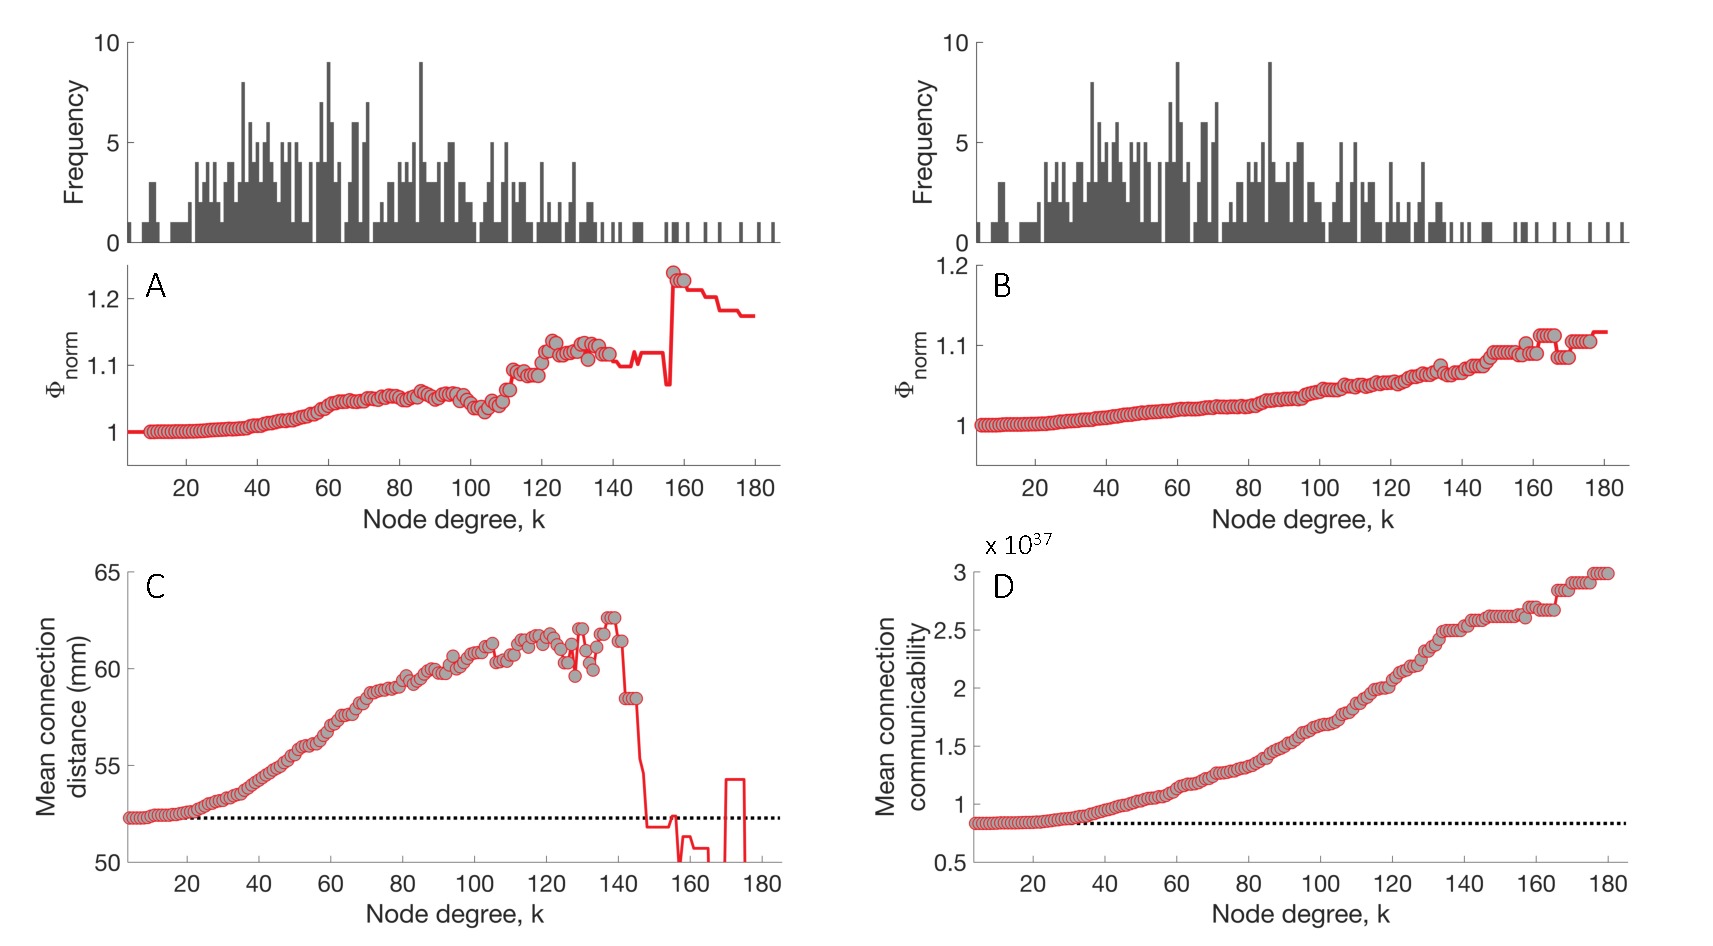
\includegraphics[width=1\textwidth]{Chapter5/Ch5Fig3.pdf}% This is a *.eps file
\end{center}
\caption{\textbf{Rich club organisation of the connectome.}
Top: the degree distribution of the connectome. Bottom:
(A) Normalized topological rich club coefficient $\Phi_{norm}$; $\Phi_{norm} >1$ indicates that hubs are more densely interconnected than expected by chance; circles indicate values that are significantly higher compared to an ensemble of 1000 degree-matched null networks ($p < 0.05$).
(B) Normalized weighted rich club coefficient ($\Phi_{norm}^{w}$); $\Phi_{norm}^{w}>1$ indicates that connections between hubs are stronger than expected by chance; circles indicate values that are significantly higher than an ensemble of 1000 topology-matched null networks ($p < 0.05$). Mean Euclidean separation distance between connected hub regions (C) and mean connection communicability (D) as a function of the degree, \textit{k}, at which hubs are defined (as regions with degree $> k$); The mean connection distance and communicability values across all network links shown as a dotted black line; circles indicate values significantly greater than across all other pairs of connected regions (right-tailed Welch’s $t$-test, $p < 0.05$).}
\label{fig:Ch5Fig3}
\end{figure}

Using the weighted rich club coefficient ($\Phi_{norm}^{w}$), we quantified whether connections between hubs tend to be stronger than expected by chance. In this analysis, the null networks were generated by randomising the connection weights while preserving the network topology. Such randomisations allow to assess the weighted rich club effect that is independent from the topological rich club \citep{Alstott2014}. The continuous increase in the weighted rich club coefficient across degree thresholds (Figure \ref{fig:Ch5Fig3}B) indicates that, in addition to being more densely interconnected as defined by the topological rich club, hub regions preferentially share stronger connections.

Compared to other connections within the network, connections between hubs display a higher mean connection length (Figure \ref{fig:Ch5Fig3}C). The high interconnectivity between hubs as well as their tendency to share stronger and longer distance connections indicate the high wiring-cost associated with establishing and maintaining hub connectivity. These properties counter the general trends across the brain observed in different species where connection probability \citep{Arnatkeviciute2018,Fornito2019,Fulcher2016} and weight \citep{Betzel2018} tend to decrease with distance.

The topological centrality of each edge serves as a proxy for its functional importance in network communication and can be quantified using a measure of communicability which accounts for the contribution of all possible paths between a pair of nodes [and is consistent with a diffusive model of signal propagation; see \citep{Avena-Koenigsberger2017}]. Here we show that the mean connection communicability increases as a function of degree (Figure \ref{fig:Ch5Fig3}D) suggesting that connections between hubs are likely to mediate a high proportion of signal traffic within the brain. Collectively, these results indicate that, rich links are particularly costly and functionally important elements of the connectome, as has previously been shown in human \citep{VandenHeuvel2011} and other species \citep{Arnatkeviciute2018,Fulcher2016,Towlson2013}. Having established the importance of hub connectivity we now turn to investigate the genetic correlates associated with hub connectivity.

\subsection{Heritability}

We start with quantifying the degree to which genes influence brain connectivity using a connectome-wide heritability analysis (see section \nameref{sec:Heritability}). Biometric models (ACTE, ACE, AE, CE, E) of individual variability in the connection strength were fitted to every edge to partition the phenotypic variability into several factors: additive genetic (A); common environmental (C); twin specific common environmental (T) and unique environmental (E). The best-fitting model for every edge was determined using the Akaike information criterion \citep{Akaike1998}. For the majority of connections, the selected model included the additive genetic component (AE $= 48\%$, ACTE $= 17\%$, ACE $<1\%$), while $34\%$ of connections did not display a significant genetic contribution (E $= 24\%$, CE $= 10\%$).

\begin{figure}[h!]
\begin{center}
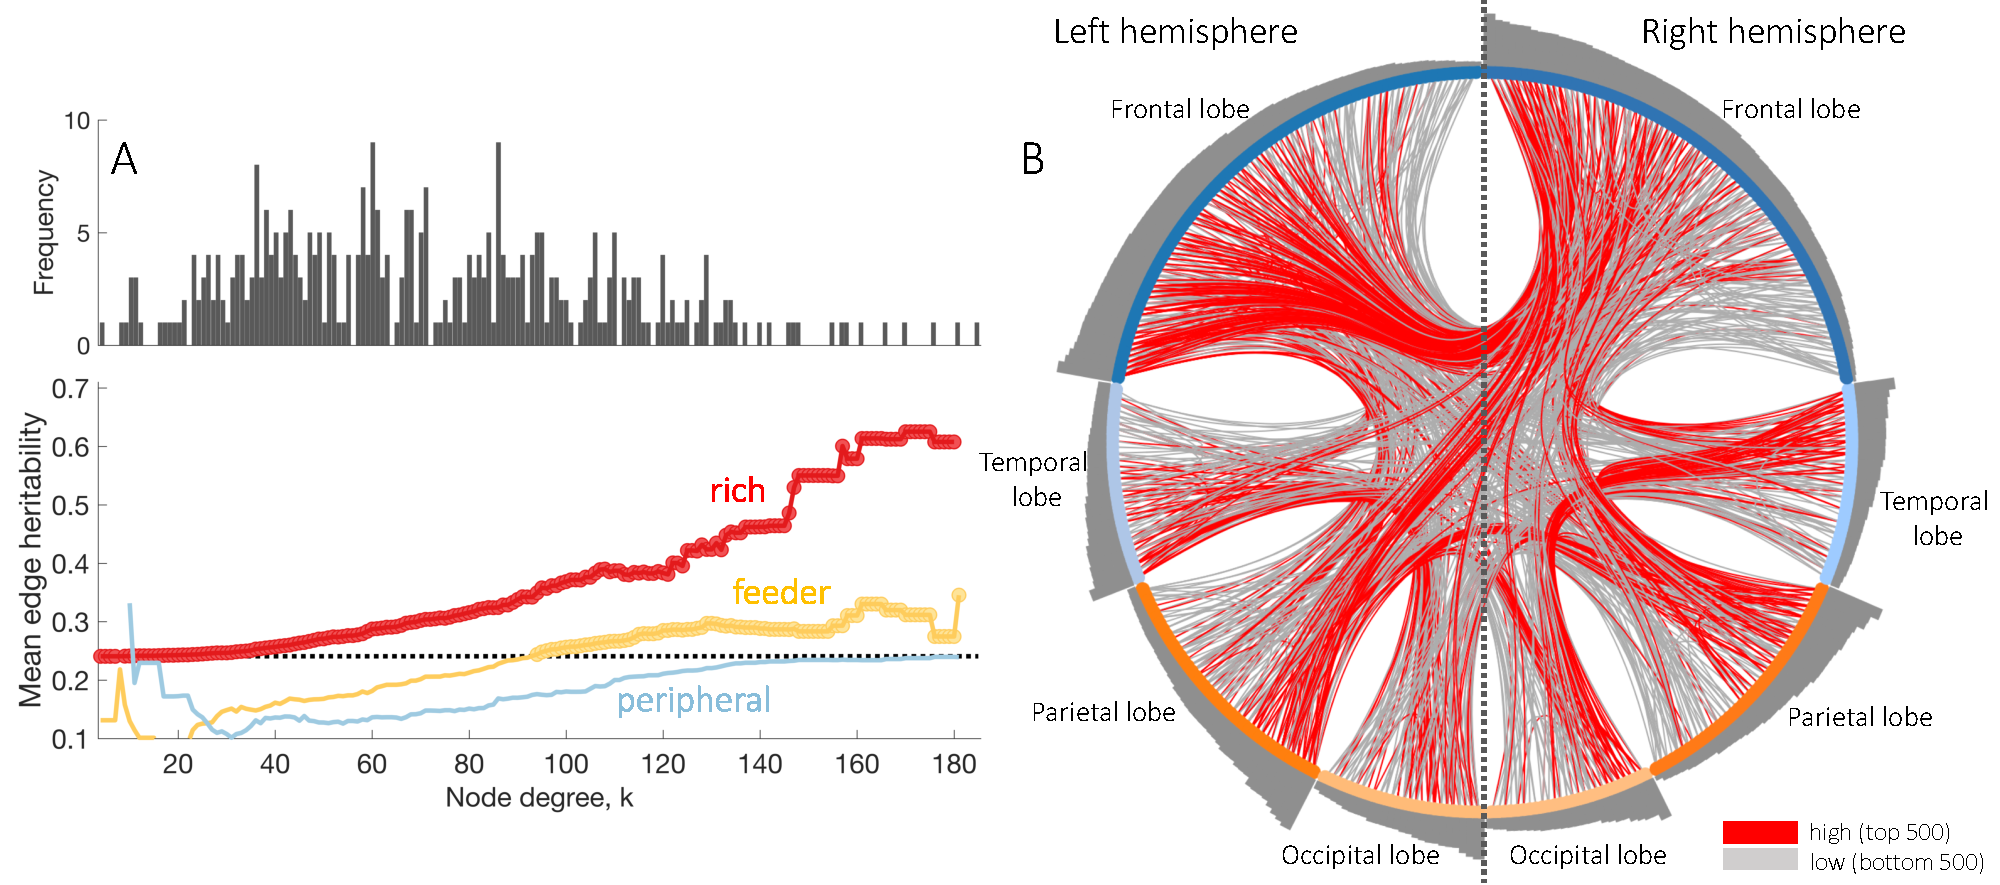
\includegraphics[width=1\textwidth]{Chapter5/Ch5Fig4.pdf}% This is a *.eps file
%https://immersive.erc.monash.edu/neuromarvl/?save=7ecb3a65-228e-4299-bcd4-2c65423741a8_130.194.90.94
\end{center}
\caption{\textbf{Rich links show an increased heritability.}
(A) Top: The degree distribution of the representative group-level connectome. Bottom: Mean edge heritability for `rich' (hub -- hub), `feeder' (hub -- non-hub), `peripheral' (non-hub -- non-hub) connections as a function of degree threshold, \textit{k} used to define hubs. The mean heritability across all network links shown as a dotted black line. Circles indicate a statistically significant increase in heritability in a given link type compared to the rest of the network (one-sided Welch’s $t$-test, $p < 0.05$).
(B) Connectogram showing the heritability for the 500 highest and 500 lowest values. Connections (lines) between brain regions (circles) are coloured according to their heritability estimates. Considering that $34\%$ of all connections exhibit 0 heritability, 500 connections were selected at random for visualisation purposes. Brain regions are organised by hemisphere and lobe with the frontal regions represented at the top of the plot. Nodes are sorted by degree (shown in bars) and coloured by lobe.}
\label{fig:Ch5Fig4}
\end{figure}

As a result, based on the best fitting model estimate, we evaluate the narrow sense heritability (the proportion of variance attributable to additive genetic factors) and investigate how it varies across different connection types defined according to rich club status. For a given hub threshold (degree $> k$), we define each node as a hub (degree $> k$) or a non-hub (degree $\leq k$) and then classify each connection as `rich' (hub -- hub), `feeder' (hub -- non-hub) or `peripheral' (non-hub -- non-hub) (see Figure \ref{fig:Ch5Fig1}). The mean heritability for every link type across a range of degree thresholds is shown in Figure \ref{fig:Ch5Fig4}A. The statistically significant increase in heritability for a particular link type compared to the rest of the network (one-sided Welch’s $t$-test, $p < 0.05$) is indicated by filled circles. The mean heritability for rich links increases as a function of degree, especially within the topological rich club regime, indicating that the strongest genetic influences are for the connections between the most highly inter-connected hubs. As expected, connections involving one hub (feeder links) also demonstrate a slight increase in the mean edge heritability across a range of degree thresholds, supporting the graded nature of the effect. Connections between non-hub regions (peripheral links) exhibit the lowest heritability across the degree distribution. Figure \ref{fig:Ch5Fig4}B further displays the anatomical distribution of connections with the highest and lowest heritability estimates. The most heritable connections, despite of their anatomical position, tend to be located between the high degree nodes while the edges with the lowest genetic contributions are more likely to connect lower degree regions.

\subsection{Polygenic variation}

Next, combining the DWI and genotype data from the Monash Cohort, we examined the relationship between connectivity and the polymorphic genetic variation. Connections were defined by applying the previously defined criteria (see section \nameref{sec:DWI}) resulting in a 20\% density group-representative connectome comprising \num{12924} unique connections between 360 functionally specified regions. As with the HCP data, the connectome exhibited both topological and weighted rich club organisation (see \ref{app:AppendixCh5_3}). Hubs were defined as regions with $k > 110$ based on the topological rich club organization of the group representative connectome showing a consistent increase in the normalized rich club coefficient at high degree.

To test whether cumulative polygenic risk for psychiatric disorders (ASD, bipolar disorder, major depression, schizophrenia and ADHD) is associated with the connectivity strength, for every connection within the connectome we used a partial correlation coefficient between the connection weight and PGRS across subjects controlling for participants sex and age. We expected that an increased genetic risk for psychiatric disorders would be preferentially associated with reduced hub connectivity. In line with our hypothesis, the correlations between the normalized connection weights and polygenic risk scores for all disorders demonstrated a similar tendency with the values for rich links decreasing as a function of \textit{k} threshold (Figure \ref{fig:Ch5Fig5}). In the case of ASD and bipolar disorder the decrease in the association for rich links started at relatively moderate thresholds (Figure \ref{fig:Ch5Fig5}D,E) with significantly lower values at the beginning of the topological rich club regime ($k>110$, one-sided Welch's $t$-test, $p < 10^{-10}$) whereas for other disorders (Figure \ref{fig:Ch5Fig5}A-C) significant differences were observed only at the very end of the degree distribution. Thus, higher polygenic risk for mental disorders, particularly ASD and bipolar disorder, is associated with decreased connectivity strength between network hubs.

\begin{figure}[h!]
\begin{center}
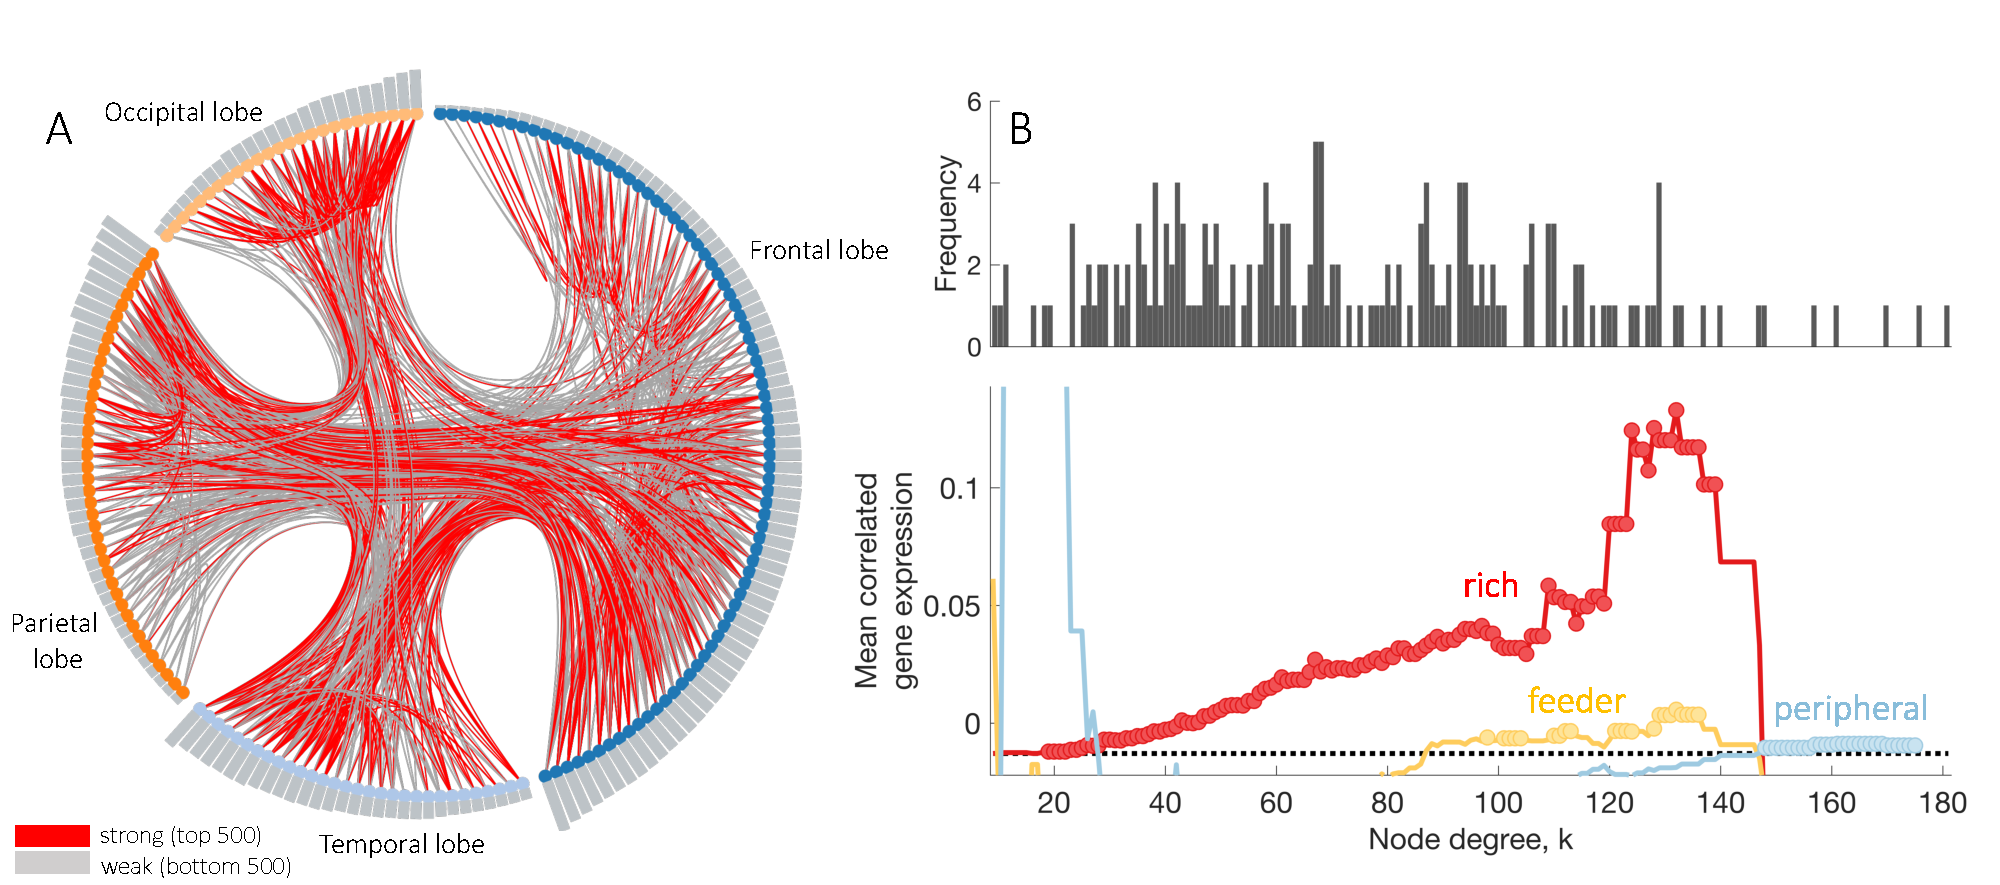
\includegraphics[width=1\textwidth]{Chapter5/Ch5Fig5.pdf}% This is a *.eps file
%https://immersive.erc.monash.edu/neuromarvl/?save=7ecb3a65-228e-4299-bcd4-2c65423741a8_130.194.90.94
\end{center}
\caption{\textbf{Rich links show distinct correlation patterns in relation to the genetic risk for disorders and genetic scores for IQ.}
Top: Degree distribution, \textit{k}, of the connectome. Bottom: Mean partial correlation (Spearman) coefficient between the connection weight and polygenic scores for schizophrenia (A), major depression (B), ADHD (C), ASD (D), bipolar disorder (E) and IQ (F) for each connection type as a function of \textit{k}. The mean partial correlation across all network links is shown as a dotted black line; Circles indicate a statistically significant decrease (A-E) and increase (F) in correlation coefficient in a given link type relative to the rest of the network (one-sided Welch's $t$-test, $p < 0.05$).}
\label{fig:Ch5Fig5}
\end{figure}

We also investigated the association between connectivity strength and polygenic scores for IQ expecting the opposite association, namely, that higher polygenic scores will be related to increased hub connectivity. First, we tested whether polygenic scores derived based on the latest publicly available GWAS for IQ \citep{Savage2018} were informative of the IQ scores in our sample. Indeed, the polygenic scores at $p_{T} = 0.05$ were able to explain $6.2\%$ variance in IQ measures in our sample ($p = 3.6 \times 10^{-7}$), comparable with previously found associations between PGS and phenotypic traits \citep{Euesden2015} suggesting a meaningful association with the phenotype. As shown in Figure \ref{fig:Ch5Fig5}F, the average correlation between the polygenic scores and connectivity strength was the highest for rich followed by feeder links while no increase was observed in peripheral connections. This relationship suggests a positive association between the genetic scores for IQ and connection strength between hubs. In other words, people with higher genetic scores for IQ, on average, have an increased connectivity strength for connections between hubs. Across the topological rich club regime ($k > 110$), the associations are stronger for rich compared to feeder links as well as for feeder compared to peripheral (Welch's $t$-test; all $p<0.01$).


Despite the association in all cases being relatively weak, the opposite relationships observed in the case of the polygenic scores for disorders and IQ imply a meaningful trend. Together, these results suggest that the effects of the structural DNA variation evaluated through the cumulative effect using polygenic scores converge on hubs and exemplify the same trend observed in the analysis of heritability.

\subsection{Transcriptional coupling}

Finally, we investigated the transcriptional properties of connectivity by evaluating the transcriptional coupling between brain regions, as quantified using CGE, across different link types. The analysis was focused to the left hemisphere due to the limited coverage of the AHBA (see section \nameref{secGeneExpression}). Figure \ref{fig:Ch5Fig6}A visualizes the anatomical distribution of connections between the region pairs with the strongest (highest positive CGE) and weakest (lowest absolute CGE) transcriptional coupling. The strongest transcriptional coupling is more likely to occur between higher degree nodes. To further investigate the patterns of transcriptional coupling between different link types, we plot the mean CGE for every link type as a function of degree threshold (Figure \ref{fig:Ch5Fig6}B). The plot reveals that CGE for rich links increases as a function of degree, with a sharp increase observed within the topological rich club regime. Feeder links showed only a very marginal increase at the highest degree thresholds, while peripheral links had the lowest CGE. These CGE findings thus mirror those obtained in the heritability and polygenic score analysis.

\begin{figure}[h!]
\begin{center}
\includegraphics[width=1\textwidth]{Chapter5/Ch5Fig6.pdf}% This is a *.eps file
%https://immersive.erc.monash.edu/neuromarvl/?save=7ecb3a65-228e-4299-bcd4-2c65423741a8_130.194.90.94
\end{center}
\caption{\textbf{Rich links show an increased correlated gene expression.}
(A) Connectogram showing the anatomical distribution of connections between the regions with the strongest (top 500 highest positive) and weakest (lowest absolute) transcriptional coupling. Connections (lines) between brain regions (circles) are coloured according to the correlated gene expression between the regions they connect. Brain regions are organised by the lobe (shown in node colour) and sorted by degree (shown in bars). 
(B) Top: The degree distribution of the left hemisphere group-level connectome. The degree for every region is based on the whole brain connectivity. Bottom: Mean CGE for `rich' (hub -- hub), `feeder' (hub -- non-hub), `peripheral' (non-hub -- non-hub) connections as a function of degree threshold, \textit{k} used to define hubs. The mean CGE across all network links shown as a dotted black line. Circles indicate a statistically significant increase in CGE in a given link type compared to the rest of the network (one-sided Welch's $t$-test, $p < 0.05$).}
\label{fig:Ch5Fig6}
\end{figure}

We next investigated whether any particular functional groups of genes are driving the transcriptional coupling between hubs. Each gene was assigned a score quantifying its contribution towards the increase in CGE in rich compared to peripheral links, as these two categories present the most topologically distinct connection types (see section \nameref{sec:CGE}). For this analysis edges within the topological rich club regime (degree $> 105$) were defined as rich and links between regions with degree $\leq105$ as peripheral. We performed a gene score resampling (GSR) analysis (see section \nameref{sec:enrichment}) to determine whether high-scoring genes were enriched in any gene ontology (GO) biological process categories. A total of 41 category showed a significant ($p<0.05$, FDR corrected) increase in the CGE for rich links. These categories included those related to cell metabolism including `ATP synthesis coupled electron transport', `oxidative phosphorylation', `cellular respiration' and `nucleotide phosphorylation', among others (see Figure \ref{fig:Ch5SFig14}). The involvement of metabolism-related genes in driving the increased CGE between hub regions is in line with their high energetic demands \citep{Bullmore2012,Collin2014,Liang2013a,Tomasi2013} and match previous analyses of CGE in mouse \citep{Fulcher2016}, and spatial gene-expression maps in human \citep{Vertes2016b}.

\section{Discussion}

Hubs are thought to represent costly but functionally valuable elements of brain networks \citep{VandenHeuvel2012} that demonstrate conserved organization across a range of species and scales \citep{Harriger2012,Towlson2013,VandenHeuvel2011,Zamora-Lopez2010}. Here we confirm that connections between hubs in the human brain are topologically central and costly, as previously demonstrated \citep{VandenHeuvel2012}, and show that hub connectivity is likely to be under tight genetic control. Specifically, we find that compared to the rest of the network, connections between hubs are more heritable; that hub regions display increased transcriptional coupling despite being separated by longer distances; that increased genetic risk for psychiatric disorders is associated with reduced hub connectivity; and higher genetic scores for IQ are related to increased connectivity strength between hubs. Together, these findings demonstrate a relationship between the large-scale brain connectivity and genetics, with the most pronounced effects on edges involving network hubs -- regions that are among the most costly and functionally valuable elements of the connectome.

Early genetic studies have successfully implemented heritability analyses to quantify genetic contributions towards a range of imaging derived phenotypes \citep{Colclough2017,Fornito2011,Peper2007,Roshchupkin2016,Shen2014,Sinclair2015,Sudre2017,Thompson2001}, demonstrating moderate to high degree of genetic influences. In line with the general principles of brain organisation suggesting a trade-off between minimising the wiring cost and maximising the communication efficiency, prior evidence of a strong genetic contribution towards regional cost-efficiency in functional networks \citep{Fornito2011} supports the hypothesis that brain networks have evolved to satisfy the competitive selection criteria of minimizing cost and promoting efficient, adaptive performance. Hub connectivity plays a central role in how nervous systems negotiate this trade-off \citep{VandenHeuvel2013b}  and, as our findings demonstrate, is under substantial genetic control. Indeed, the gradual increase in heritability for rich links followed by feeder connections across a range of degree thresholds indicates a graded nature of the effect such that the genetic control over brain connectivity is increasing with increasing topological connection centrality.

Having established that the contributions of additive genetic factors converge on connections between hubs we aimed to investigate how inter-individual differences in hub connectivity relate to the structural DNA variations between people. We evaluated the associations between polygenic scores for five major psychiatric disorders and structural connectivity and found that genetic susceptibility for illness is preferentially linked to reduced connection strength between hubs. Under the assumption that hubs form a putative backbone for brain communication \citep{Harriger2012,Towlson2013,VandenHeuvel2011,VandenHeuvel2013b}, decreased connectivity strength between them might indicate a reduced integrative capacity that is linked to the increased genetic predisposition to psychiatric disorders. Consistently negative associations across disorders were countered by the positive trend observed in relation to the polygenic scores for IQ indicating an increased connectivity strength between hubs in subjects with the higher genetic scores for IQ. Although the associations are moderate, consistent with the bulk of polygenic associations reported thus far \citep{Alloza2018,Dezhina2018,Liu2016a,Sadeh2018,Wang2017}, the opposite direction of the associations for disorders and IQ suggests that different genes exert opposing effects on hub connectivity, ultimately resulting in the expression of distinct behavioural phenotypes. Although, the utility of the polygenic scores in the field of imaging genetics has been questioned \citep{Reus2017}, a number of studies have identified associations between PGS and cortical gyrification \citep{Liu2016a}, functional connectivity \citep{Dezhina2018,Sadeh2018,Wang2017} and longitudinal changes in white matter properties \citep{Alloza2018}. More specifically, in line with the directionality of our results, genetic predisposition to major depression was found to be associated with decreased global white matter integrity \citep{Whalley2013} whereas higher genetic scores for IQ showed a positive association with global FA \citep{Jansen2018}. Our findings indicate that polygenic liability for psychiatric disorders, and genetic predisposition to adaptive traits such as IQ, is preferentially associated with functionally critical hub connectivity.

Next, we aimed to replicate the previous findings in mouse \citep{Fulcher2016} and \textit{C.elegans} \citep{Arnatkeviciute2018} demonstrating increased gene expression similarity between hubs. Investigating how gene expression patterns track macroscale brain network organisation in human became possible through the availability of the Allen Human Brain Atlas \citep{Hawrylycz2012}. In the past few years, a range of brain network properties in human have been related to gene expression \citep{Cioli2014b,Forest2017,Goel2014,Richiardi2015,Vertes2016b}. Replicating the previous findings in mouse \citep{Fulcher2016} and \textit{C.elegans} \citep{Arnatkeviciute2018}, consistently increasing CGE between hubs suggests some intrinsic genetic similarity between those regions despite their disparate anatomical locations. Moreover, the involvement of metabolism-related genes in driving this transcriptional coupling mirrors the findings in both mouse \citep{Fulcher2016} and human \citep{Vertes2016b} indicating a conserved transcriptional signature supporting high energetic requirements of hub areas \citep{Liang2013a,Tomasi2013} that transcends different species. This result is consistent with evidence that hubs are metabolically expensive \citep{Vaishnavi2010,Varkuti2011}. Indeed, the high metabolic demands of hub regions may increase their sensitivity to metabolic distress, making these areas vulnerable to the effects of injury or disease \citep{Crossley2014,Fornito2015}. It is possible that CGE of metabolic genes may be related to similarities in the microcircuitry of hub regions, given that the AHBA data are derived from bulk tissue samples and do not distinguish expression patterns of different cell types. Single-cell sequencing \citep{Lein2017} would shed some light on this possibility.

Providing such unprecedented opportunities for new research, the usage of publicly available databases such as AHBA pose several challenges as integrating gene expression measures derived from an atlas together with imaging data requires substantial consideration \citep{Arnatkeviciute2019,Fornito2019}. One of the most critical aspects in investigating the transcriptional correlates of a spatially varying brain imaging phenotype such as connectivity, are the spatial properties of gene expression. Spatial autocorrelations of gene expression have been observed across multiple species \citep{Arnatkeviciute2018,Burt2018,Fornito2019,Fulcher2016} with regions in close proximity exhibiting more similar gene expression. Whereas spatial autocorrelation of gene expression is an interesting question in itself, most studies relating gene expression to the imaging derived phenotypes aim to evaluate the relationships beyond simple spatial patterns. This can be achieved by statistically controlling for these relationships \citep{Fakhry2015a,Fulcher2016} or by evaluating the statistical significance of the result based on the spatially constrained null models \citep{Burt2018,Romero-Garcia2018,Whitaker2016a,Vasa2018,Vertes2016b}. Here we account for the spatial relationship by approximating it with an exponential trend and analysing the spatially corrected CGE as the residuals from a bulk spatial trend estimated as an exponential fitted to all pairs of brain regions. Therefore, the observed transcriptional similarity between hub regions does not result from the general spatial trends in gene expression and thus provides additional information regarding their functional role.

\section{Conclusions}
In this work we combined three different approaches spanning several levels of genetic inference to systematically evaluate genetic contributions to brain connectivity. We demonstrate that functionally important connections between topologically central network hubs are under stronger genetic control compared to more topologically peripheral links. At the level of structural DNA variation, we show that polygenic liability for psychiatric disorders is preferentially associated with decreased connectivity strength between hubs whereas higher polygenic scores for IQ are indicative of increased hub connectivity. Linking gene function and brain-wide connectivity we show that hub regions display a tightly coupled gene expression. This transcriptional coupling is driven by metabolism-related genes. Together, our findings demonstrate a direct link between molecular function and the large-scale organisation of the human connectome.
  
  \clearpage
  %!TEX root = ../Thesis.tex
\chapter{General discussion and concluding \\ remarks}
\label{ch:Discussion}
\fancyhead[R]{\textit{Chapter.} \textit{\thechapter: }\textit{General discussion and concluding remarks}}
%\fancyhead[ER]{\bf Ch. \thechapter~INTRODUCTION \& OVERVIEW}

\section{General discussion}
The overarching aim of this thesis was to investigate the molecular basis of large-scale brain connectome organisation, with a particular focus on the genetic underpinnings of brain network hub connectivity. The critical role that hubs are assumed to play in cognitive performance \citep{Buckner2009}, coupled with the susceptibility of these regions to a range of brain disorders \citep{Bassett2009a,Crossley2014,Fornito2015} highlights their importance for integrated brain function. The striking conservation of network hubs and rich-club organization across species and scales, together with the consistently high centrality and cost of these network elements \citep{VandenHeuvel2016}, suggest that hub interconnectivity may have evolved to satisfy competitive selection criteria of minimising connection costs while maintaining integrated communication between neural elements \citep{Bullmore2012}. Understanding the genetic basis of hub connectivity could thus shed light on key evolutionary principles for brain networks, the molecular basis of higher-order, integrative brain function, and genetic liability for brain disease.

This thesis examined the link between genetics and hub connectivity across two disparate spatial scales: the microscale of cells and synapses in \textit{C.elegans} and the macroscale of brain regions linked by white matter bundles in the human. As part of the latter analysis, a detailed pipeline for relating human neuroimaging and gene expression data was developed. The following sections outline some general implications of the major findings.

\subsection*{Hub connectivity is associated with a highly conserved transcriptional signature}

As previously demonstrated in the mesoscale mouse connectome \citep{Fulcher2016}, Chapter 2 showed that hub neurons in the \textit{C.elegans} connectome display increased similarity of gene expression profiles. Findings presented in Chapter 5 demonstrate that a similar increase in transcriptional coupling between hub regions is also evident in the macroscale human connectome. This consistency is striking given the large differences in resolution scales (worm: cells and synapses; mouse: cell populations and axons; human: brain regions and white matter bundles), connectome mapping methods (worm: electron microscopy for; mouse: viral tract-tracing; human: DWI), and gene expression quantification (worm: binary expression indicators derived from the previous literature; mouse: cellular resolution \textit{in-situ hybridisation}; human: bulk tissue microarray). Both mouse and human analyses indicated that the strongest contributions to elevated CGE between pairs of connected hubs come from genes regulating oxidative metabolism. This specific result could not be replicated for \textit{C.elegans}, as expression data for such genes were not available.

A key aspect of this apparent transcriptional signature of hub connectivity is that it counters the more general trend in the brain, in which CGE and connection probability decline as a function of distance between regions. In contrast, hubs have higher CGE and are more likely to be connected despite being, on average, separated by longer physical distances. This distinctive increase in CGE between hub regions could arise from multiple sources, including cellular and microcircuitry properties of hub regions. For example, non-human primate studies have identified that hub regions have lower neural cell density \citep{Beul2017,Scholtens2014}. Higher levels of regional connectivity have also been associated with a range of microscopic properties in macaque brains indicating increased neuronal complexity including more elaborate pyramidal dendritic branching, higher total spine count and larger soma size \citep{Scholtens2014}. Moreover, regional cytoarchitectural properties have been related to their pairwise laminar-projection profiles linking local microcircuits to their long-range connectivity \citep{Barbas,Barbas2015}. The cell-specific analysis of \textit{C.elegans} counters a simple cell density explanation, indicating the important role of specific cell types. The analysis of gene expression in \textit{C.elegans} shows that the functional identity of hub neurons is a significant factor in driving the increase in CGE between them. Future work investigating the cell-specific transcriptional properties of hub regions is required in order to test this hypothesis in higher order animals.

\subsection*{Hub connectivity in the human connectome is under tight genetic control and is linked to genes for intelligence and mental illness}

Relating imaging to gene expression data provides a way for identifying how spatial patterns of gene expression track spatial variations of network phenotypes. However, they do not offer insight into whether or which genes regulate inter-individual differences in hub connectivity. Chapter 5 thus combined two other commonly used methods for characterizing genetic influences on a given trait -- heritability analysis of twin data and polygenic score analysis of structural DNA variants.

The heritability analysis revealed that individual differences in the hub connectivity strength are under strong genetic control: average heritability of  rich links is significantly higher compared to both feeder and peripheral links. Moreover, feeder connections showed significantly higher heritability compared to peripheral links, demonstrating the graded nature of the effect, where genetic contribution is increasing with increasing topological centrality of the connections. This result indicates that genes play a major role in shaping connectivity microstructure that appears to be highly selective for the connections between connectome hubs. This high heritability of hub connectivity is consistent with the hypothesis that the apparent trade-off between wiring cost and adaptive function may be strongly concentrated on the arrangement of hub connections \citep{Bullmore2012}. This result implies that genes, by virtue of their effect on hub connectivity, may play a key role in determining how individual brains negotiate the trade of between cost minimization and adaptive network topology. 

The genetic primacy of hub connections is supported by developmental considerations [for a review see \citep{Oldham2018}]. In \textit{C.elegans}, hub neurons are born at the earliest stages of the development \citep{Varier2011}, prior to evidence of coordinated movement in the animal. Structural hubs within  human brain networks also tend to emerge early in development, with studies demonstrating the presence of hubs in superior frontal, superior parietal, and occipital regions as early as 30 weeks gestational age \citep{Ball2014}. Hubs in preterm infants also form a highly interconnected rich-club, with most changes in the last 10 weeks of gestation occurring between hubs and other regions, rather than concentrating on the relatively mature rich connections between hubs \citep{Ball2014}. Furthermore, only minor changes in the connectivity strength between the putative core elements of the brain have been observed during the third trimester of fetal development \citep{Batalle2017}, indicating the early formation and relative consistency of hub connections in the human brain. Thus, the basic binary topology of hub connectivity may be established early, but these connections may undergo a protracted period of development, resulting in changes to the weighted topology of the network \citep{Baker2015a,Oldham2018}.

The PGS analysis revealed that genetic liability for a range of psychiatric disorders is preferentially related to reduced connectivity between hub regions. At the same time, higher genetic scores for IQ showed the opposite relationship, indicating that, on average, subjects with higher genetic scores for IQ have increased connection strength between hubs. This suggests that genes involved in driving inter-individual differences in hub connectivity are implicated in a broad range of phenotypes, including mental illness and general intelligence.
Considering that hubs form a backbone for brain communication \citep{Harriger2012, VandenHeuvel2011,VandenHeuvel2013b}, such relationship converging on connections between hub regions might be related to the differences in the integrative capacity of the brain that is linked to the increased genetic predisposition to psychiatric illness.

\subsection*{Standardized workflows are required for relating gene expression and \\neuroimaging data}

The capacity to link brain imaging data to gene expression measures is a recent innovation, possible only with the advent of brain-wide genome-wide gene expression atlases in different species [\citep{Harris2010,Hawrylycz2012,Lein2007a}, for a review see \citep{Keil2018}]. Although a growing number of studies are bridging the two types of data, there are no standard practices in the field and many data processing options are available. Chapter 4 conducted the first systematic survey of such options and found that processing choices can significantly affect the resulting data. For example, some procedures that are important for the meaningful biological interpretation of the results are often ignored in the literature, including  probe-to-gene re-annotation and the appropriate investigation of the spatial properties of gene expression. Whereas most of the processing choices require further consideration and should be tailored to particular research questions, it is necessary to ensure the implementation of comparable processing pipelines allowing to draw links between findings across different studies. The processing pipeline presented in this paper has been made publicly available allowing researchers to make any desired modifications. Moving forward, it will be important to work towards unified data processing methods when integrating brain-wide gene expression atlases with other modalities across species. 

\section{Limitations and future directions}

Despite the consistency of genetic influences on hub connectivity identified in this thesis, each study has a number of limitations, particularly with respect to how some of the data were curated. The connectome data in \textit{C.elegans} is as close to a gold standard as possible in the field, representing the (near-)complete neuron-and-synapse wiring diagram of the organism's nervous system. However, the gene expression data was relatively incomplete, relying on the curated results stored in Wormbase \citep{Harris2010}. Being limited to  information reported in the literature, such data aggregation methods are heavily biased in their coverage, and do not allow to distinguish between the cases of missing information and absent gene expression. These drawbacks could be overcome by implementing single cell RNA sequencing to acquire genome-wide expression signatures for individual neurons, however these experiments pose a number of technical challenges including the implementation of advanced cell sorting techniques. Single-cell RNA sequencing has been performed on a larval stage of \textit{C.elegans} development \citep{Cao2017}, however it has not yet been extended to single-neuron gene expression in the adult worm.

The human gene expression data provide better genomic coverage and reasonable spatial coverage of one hemisphere of the brain, but the data are derived from six donor brains precluding a detailed investigation of inter-individual differences in gene expression patterns \citep{Arnatkeviciute2019,Hawrylycz2015}. Moreover, as the expression measures are quantified in bulk tissue samples, they may be influenced by the cellular composition of each sample \citep{Tasic2016}. Although the genetic microarray  provides a cost-effective way of quantifying gene expression in a high-throughput manner, improvements in single-cell profiling should yield more detailed and informative gene expression maps \citep{Lein2017}. Considering that a very high proportion of genes demonstrates differential expression across development \citep{Colantuoni2011}, the generation of developmentally-resolved brain-wide atlases would be informative in uncovering the relationship between the transcriptional dynamics and brain connectivity.

The analyses of large-scale connectivity in the human brain presented in this thesis rely on diffusion weighted imaging. While it is currently the only available technique allowing to noninvasively explore the structural connectivity of the human brain, results derived from such indirect approaches should be interpreted with caution \citep{Jones2013,Sotiropoulos2017}. Tractography algorithms used to infer white matter pathways from the underlying diffusion signal have known biases, including difficulties in reconstructing long-range pathways \citep{Jones2010} mainly arising due to the high proportion of voxels containing crossing fibers \citep{Jeurissen2001}. Compared to deterministic algorithms, the usage of probabilistic tractography can at least partially mitigate this issue \citep{Tournier2010}, however, the lack of ground truth measures of brain connectivity makes it difficult to balance the sensitivity and specificity of the resulting connectivity estimates \citep{Zalesky2016}. Additional challenges arise in interpreting DWI-derived measures. For example, changes in FA are frequently attributed to inherent differences in white matter integrity, however they can result from a number of other factors, including differences in axon diameter, packing density, or the number of crossing fibers in the area \citep{Jones2013,Takahashi2002}. These factors cannot be disentangled using current techniques, therefore, the ongoing development of more quantitative estimates of DWI-derived anatomical connectivity \citep{Bouhrara2016,Zhang2012} may prove useful in the future.

\newpage
\section{Conclusions}

The findings presented in this thesis contribute towards the rapidly developing field of imaging genetics by demonstrating consistent evidence for a strong genetic influence on hub connectivity. Integrating a range of data modalities across different species and scales, this work shows that the genetic influences on brain connectivity converge on topologically central and functionally important brain network hubs. More specifically, hubs tend to display increased transcriptional similarity in both micro- and macroscale brain networks. Moreover, the connection strength between hub regions in the human brain is strongly heritable and is related to polygenic liability for mental illness and high IQ. The methodological findings on integrating brain-wide gene expression and neuroimaging data highlight the importance of ensuring consistency and reproducibility in atlas-based imaging genetics research.
  

  \clearpage
  
  \appendix
  %!TEX root = ../Thesis.tex
\chapter{Hub connectivity and gene expression in \textit{C.elegans}}
\label{appendixA}

\fancyhead[R]{\textit{Appendix A:~Hub connectivity and gene expression in \textit{C.elegans}}}

\section{Expression annotations at WormBase}
\label{app:AppendixCh2_1}

Neuronal gene expression is measured as a binary indicator on WormBase \citep{Harris2010}, based on curated data collated
from many individual experiments. Expression annotations are made either ‘directly’ to individual neurons (when
an experiment indicates expression in an individual neuron), or ‘indirectly’ to broader classes of neurons like
‘interneuron’ or ‘head’ (meaning that some members of that class exhibit expression of that gene). In order to
maintain specificity of annotations, we only analysed ‘direct' annotations here.
Annotations of gene G to neuron Y are also made with varying levels of certainty:
\begin{itemize}
\item ‘certain’: G was observed to be expressed in Y,
\item ‘enriched’: G has been found to be enriched in a certain dataset through microarray, RNAseq or
proteomic analysis,
\item ‘partial’: G was observed to be expressed in some cells of a group of neurons that include Y,
\item ‘blank’: data prior to 2005, or
\item ‘uncertain’: G was sometimes observed to be expressed in Y, or G was observed to be expressed in a cell
that could be Y.
\end{itemize}

To avoid including false positives, our analysis excluded annotations labeled as ‘uncertain’.

\section{Sensitivity of correlated gene expression measures}
\label{app:AppendixCh2_2}
Measures of correlation between binary vectors can be biased by the relative proportion of ones
between two vectors. For data analysed here, data annotated to individual neurons comes from between $3$ to
$138$ expressed genes (corresponding to $0.3\%$ to $14.6\%$ of all $948$ genes considered). To ensure that our measure of correlated gene expression (CGE) is not biased by such differences in the relative proportions of expression annotations, we conducted a sensitivity analysis in which we compared the $r_\phi$ metric, Eq. \ref{eq:rphi}, with alternative
methods for quantifying correlations between binary vectors: the Jaccard index, $n_{11}/(n_{10}+n_{01}+n_{11})$, Yule's Q
coefficient, $(n_{00}n_{11}-n_{01}n_{10})/(n_{00}n_{11}+n_{01}n_{10})$, and the $\chi{^2}$, index, $N(n_{00}n_{11}-n_{01}n_{10})/(n_{0\bullet}n_{1\bullet}-n_{\bullet1}n_{\bullet0})$ \citep{Kaufman2006}, where $n_{xy}$ counts
the number of observations of each of the four binary pairwise possibilities: $n_{00}$, $n_{01}$, $n_{10}$, and $n_{11}$ (as outlined in
the main text), and the $\bullet$ symbol sums across a given variable (e.g., $n_{\bullet}= n_{00} + n_{10})$.
To evaluate bias in each CGE measure to the proportion of annotations in each expression vector, we
generated random binary vectors of length 948 containing different proportions of 1s seen in our data, ranging
from the minimum, 1, to the maximum, 150. For all pairwise combinations of proportions, we computed the CGE
measure, taking an average across $1 000$ permutations, and then recorded the resulting mean correlation value,
as plotted in Figure \ref{fig:Ch2S2_Fig}. Because all vectors are independent random binary strings, any systematic dependence of
mean CGE with annotation proportion indicates bias. The mean square contingency coefficient, (Figure \ref{fig:Ch2S2_Fig}A) and
our own novel CGE matching index, $p_{match}$ show no systematic dependence on the proportion of ones in
each vector (varying randomly within ≈ $10^{-3}$ and ≈ $0.5$ respectively). However, Yule's Q shows a negative bias for
small annotation proportions (Figure \ref{fig:Ch2S2_Fig}B) and the Jaccard index shows a strong positive bias across the full range (Figure \ref{fig:Ch2S2_Fig}C). Based on these numerical experiments, we selected mean square contingency coefficient, $r_\phi$, here, to
ensure that changes in CGE were due to matching expression patterns and not simply driven by differences in the
number of gene annotations between neurons.


\section{Correlated gene expression matching index}
\label{app:AppendixCh2_3}

Existing measures of binary correlation (described below) are symmetric between ‘0’ and ‘1’ and thus do not directly distinguish between the biologically relevant case of genes being expressed together from the case in which neither gene is expressed. We thus developed a measure of the probability, $P(m)$, that two binary strings will contain m ‘positive matches’ (i.e., m genes are expressed in both neurons), which can be computed as:


\begin{eqnarray}
	\label{eq:S3}
     P(m) = \binom{n_{2}}{m}\binom{N-n_{2}}{n_{1}-m}/\binom{N}{n_{1}},
\end{eqnarray}

for two binary expression vectors, $x_{i}$, $y_{i}$, of length N containing $n_{1}$ and $n_{2}$ 1s, respectively ($n_{1} \leq n_{2}$), with m matches ($n_{11}$). Our index, $p_{match}$, is approximately equal to the probability of obtaining as many or fewer matches than observed (weighting the probability of the observed number of matches at 0.5 for symmetry), computed as:

\begin{eqnarray}
	\label{eq:S4}
     p_{match} = \sum_{x=0}^{m-1}P(x)=P(m)/2,
\end{eqnarray}

for m positive matches.
	We verified that this index yields qualitatively similar results to the mean square contingency coefficient, $r_\phi$, (Figure \ref{fig:Ch2S3_Fig}), validating our related positive match method for scoring individual genes [as an approximately single-gene contribution to the probability score computed in Eq. \ref{eq:CBinomialProbability}].
Given the qualitative similarity of this measure to $r_\phi$, we chose to focus on $r_\phi$ throughout this work due to its ease of interpretability as a correlation coefficient ranging from -1 to 1.

\begin{figure}[h!]
  \centering{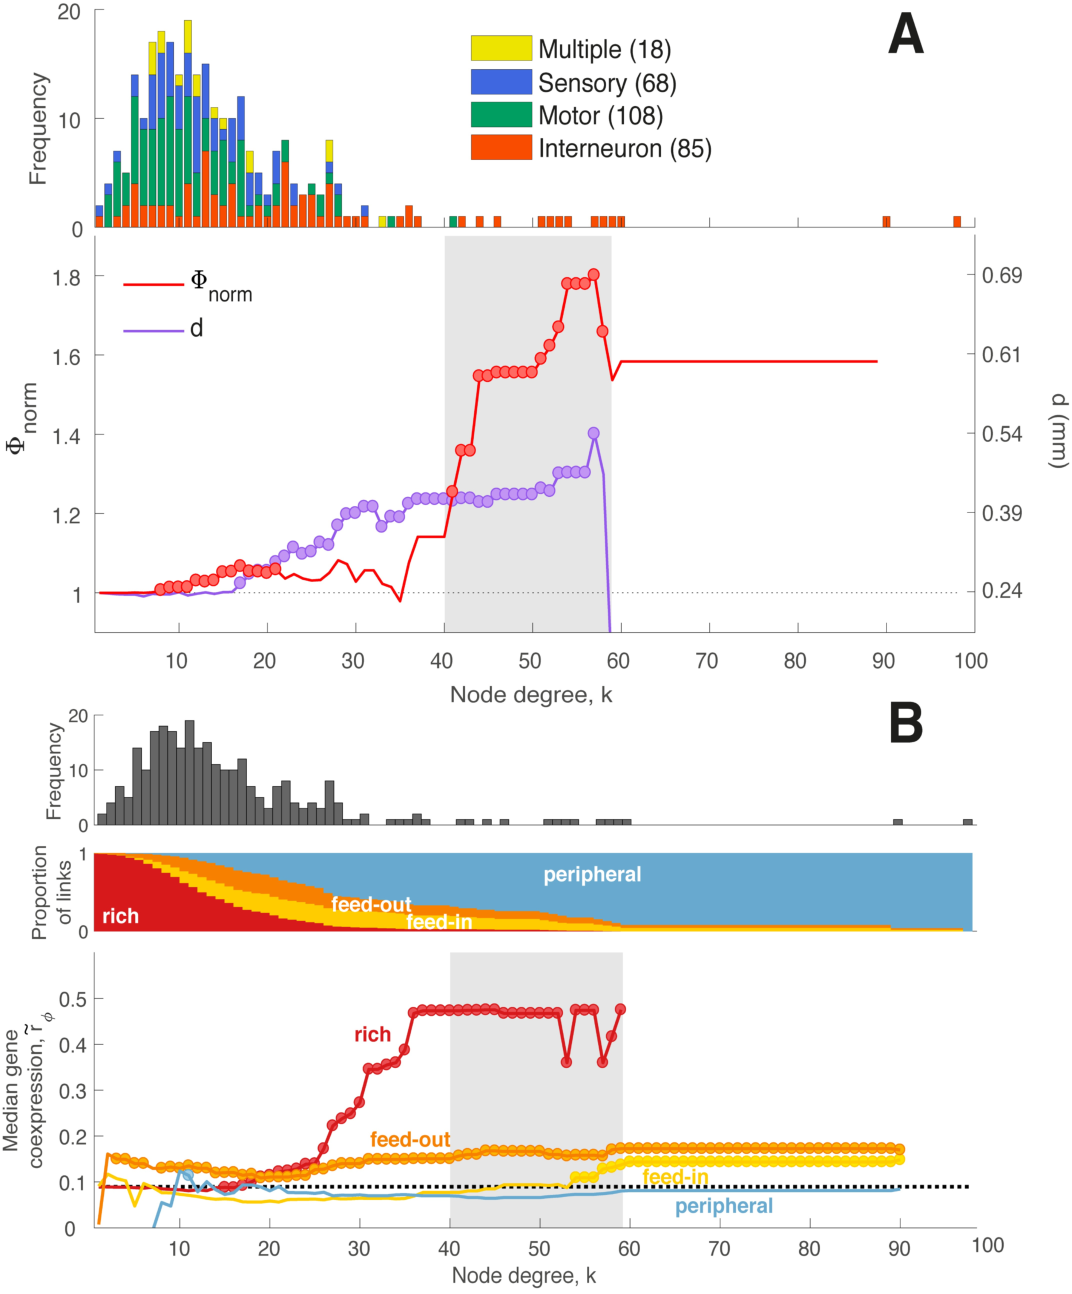
\includegraphics[width=0.6\textwidth]{Chapter2/Ch2S1fig.pdf}}
 \caption{{\bf Rich club organisation and correlated gene expression in synaptic connectivity matrix.}
(A) Rich-club organization of the synaptic \textit{C.elegans} connectome.
Top: Degree distribution of neurons, labelled to four categories: (i) interneuron (85 neurons, orange), (ii) motor (108 neurons, green), (iii) sensory (68 neurons, blue), or (iv) multiple assignments (18 neurons, yellow).
The distribution features an extended tail of high-degree neurons. Bottom: Normalized rich club coefficient, $\Phi_\mathrm{norm}$ (red), as a function of the degree, $k$, at which hubs are defined (as neurons with degree $>k$).
Also shown is the mean Euclidean separation distance, d (purple) between connected hub regions (across degree thresholds, k). $\Phi_\mathrm{norm} > 1$ indicates that hubs are more densely interconnected among each other than expected by chance, with red circles indicating values of $\Phi_\mathrm{norm}$ that are significantly higher than an ensemble of 1000 degree-matched null networks ($p < 0.05$).
Purple circles indicate where the Euclidean distance between connected pairs of hubs is significantly greater than the Euclidean distance for all other pairs of connected regions (right-tailed Welch's t-test, $p < 0.05$).
(B) Top: Degree distribution, $k$, of the synaptic \textit{C.elegans}  connectome.
Middle: proportion of connections that are: `rich' (hub $\rightarrow$ hub, red), `feed-in' (nonhub $\rightarrow$ hub, yellow), `feed-out' (hub $\rightarrow$ nonhub, orange), or `peripheral' (nonhub $\rightarrow$ nonhub, blue) as a function of the degree threshold, $k$, used to define hubs.
Note that at high $k$ most neurons are labeled as nonhubs and hence the vast majority of connections are labeled `peripheral'.
Bottom: Median CGE, $\tilde{r}_\phi$, for each connection type as a function of $k$.
The median CGE across all network links is shown as a dotted black line; the topological rich-club regime (determined from the network topology, cf. A) is shaded gray.
Circles indicate a statistically significant increase in CGE in a given link type relative to the rest of the network (one-sided Wilcoxon rank-sum test, $p < 0.05$).}

\label{fig:Ch2S1_Fig}
\end{figure}

%% FIGURE S2
\begin{figure}[h!]
  \centering{\includegraphics[width=1\textwidth]{Chapter2/Ch2S2fig.pdf}}
 \caption{{\bf Dependence of correlated gene expression measures on the proportion of positive annotations.} We plot the mean value of each metric across 1000 different pairs of random, binary vectors of length 948, which vary only in their proportion of `1's (between 0--0.15; corresponding to a number of `1's ranging from 1 to 150).
This is repeated for:
(A) mean square contingency coefficient, $r_\phi$,
(B) Jaccard index,
(C) Yule's $Q$, and
(D) our developed positive match measure, $p_\mathrm{match}$, (see \ref{app:AppendixCh2_3}).
Any systematic trend in correlation values indicates a bias driven by the proportion of positive annotations for a pair of vectors, as is seen for the Jaccard index and Yule's $Q$.
By contrast, $r_\phi$, which is used through this work, and our probability-based measure, $p_\mathrm{match}$, used to motivate individual gene scoring for enrichment analysis, show no evidence of systematic bias (note the color axis scales)}.
\label{fig:Ch2S2_Fig}
\end{figure}


%% FIGURE S3
\begin{figure}[h!]
  \centering{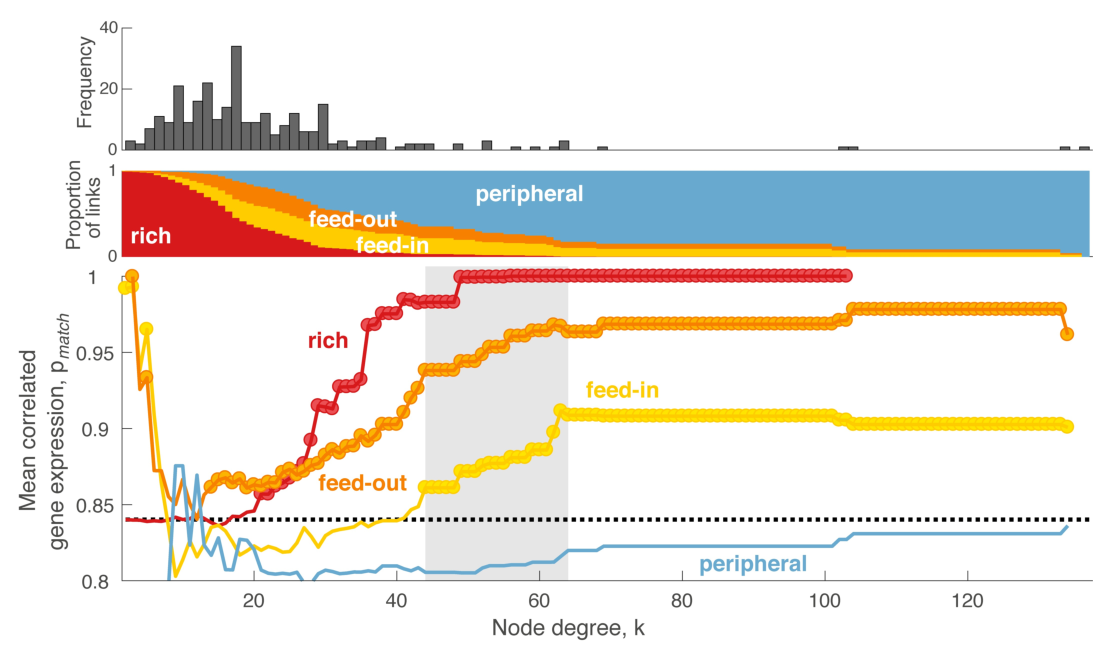
\includegraphics[width=1\textwidth]{Chapter2/Ch2S3fig.pdf}}
 \caption{{\bf Correlated gene expression measured using the positive matching probability index.} The matching probability index, $p_\mathrm{match}$, as introduced in \ref{app:AppendixCh2_3}.
\emph{Top}: Degree distribution.
\emph{Middle}: Proportion of connections that are `rich' (hub$\rightarrow$hub, red), `feed-in' (nonhub$\rightarrow$hub, yellow), `feed-out' (hub$\rightarrow$nonhub, orange), and `peripheral' (nonhub$\rightarrow$nonhub, blue) as a function of the degree threshold, $k$, used to define hubs.
Note that at high $k$, most neurons are labeled as nonhubs, and hence the vast majority of connections are `peripheral'.
\emph{Bottom}: Mean CGE calculated using similarity index from only positive matches, $p_{match}$, for each connection type as a function of $k$.
The mean CGE across all network links shown as a dotted black line; the topological rich-club regime (determined from the network topology, Figure \ref{fig:Ch2Fig5}) is shaded gray.
Circles indicate a statistically significant increase in CGE in a given link type relative to the rest of the network (one-sided Welch's $t$ test; $p < 0.05$).}
\label{fig:Ch2S3_Fig}
\end{figure}



%% FIGURE S4
\begin{figure}[h!]
  \centering{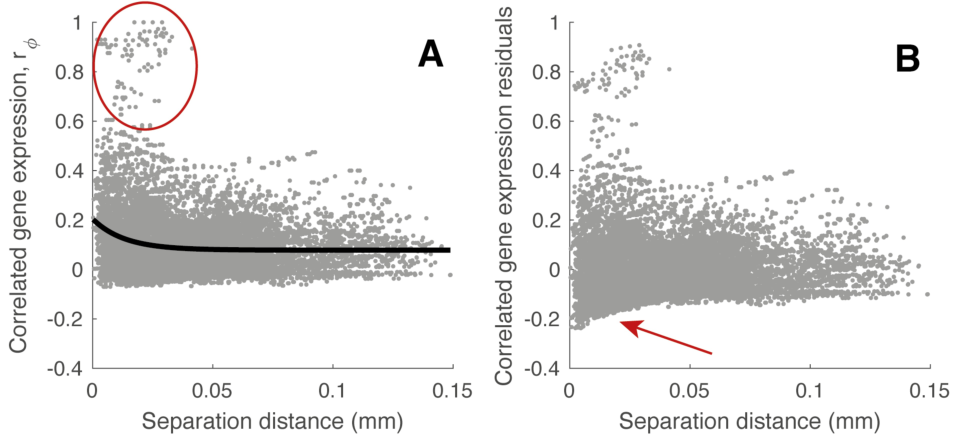
\includegraphics[width=1\textwidth]{Chapter2/Ch2S4fig.pdf}}
 \caption{{\bf Correcting for spatial effects in CGE data using a bulk exponential trend.}
  Here we consider correlated gene expression in the head, where the strongest spatial relationship exists (Figure \ref{fig:Ch2Fig4}. (A) CGE values, $r_\phi$, plotted as a function of Euclidean separation distance for all pairs of neurons within the head (gray dots), with a fitted exponential trend shown in black, $f(x) = A\exp(-\lambda x) + B$.
(B) Taking residuals from this trend does not adequately correct the spatial trend.
    Note the artifactual negative correlations indicated with an arrow.
    This indicates that the trend is not a bulk, isotropic effect, but may instead be driven primarily by a small number of neuron pairs with high $r_\phi$ at short distances ($\lessapprox 50\mu$m), indicated with a circle in (A).
For example, neuron pairs with $r_\phi > 0.8$, are all between the following classes of head neurons: CEP, IL1, OLQ, RMD, RME, RMF, SAAD, SAAV, SAB, SIA, SIB, SMB, SMD, URA, URY.}
\label{fig:Ch2S4_Fig}
\end{figure}


%% FIGURE S5
\begin{figure}[h!]
  \centering{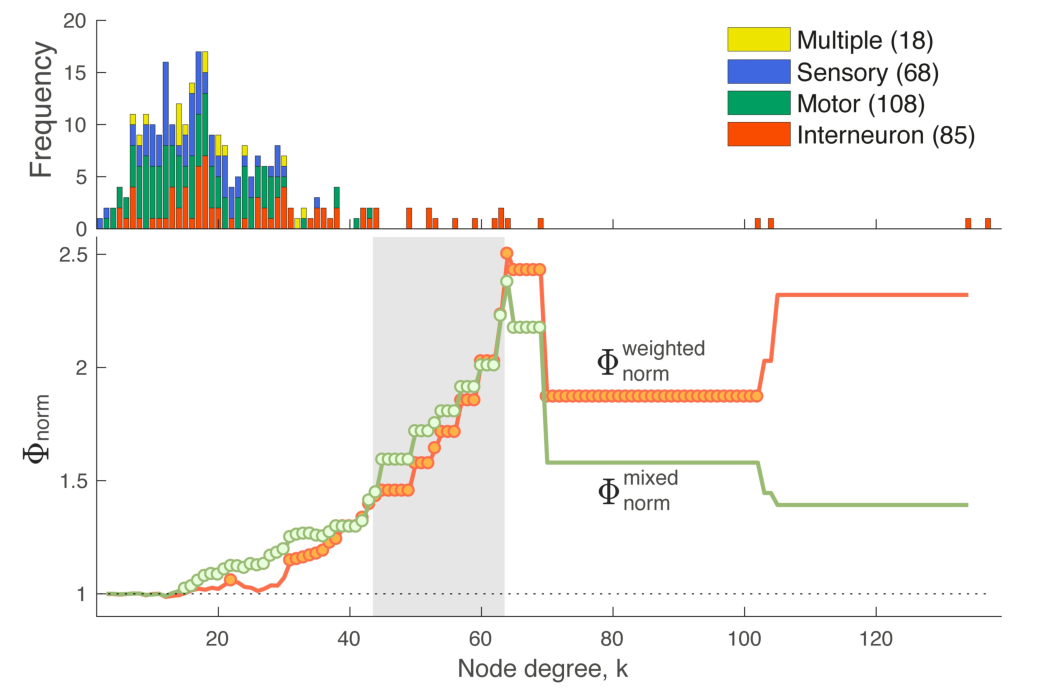
\includegraphics[width=1\textwidth]{Chapter2/Ch2S5fig.pdf}}
 \caption{{\bf Weighted and unweighted rich-club analyses yield similar results.}
   (A) Degree distribution of the \emph{C.elegans} connectome.
    Neurons are labeled to four types as in the legend.
    (B)
    Normalized weighted rich-club coefficient, $\Phi_\mathrm{norm}^\mathrm{weighted}$ (i.e., topology fixed and weights randomized in the null model, shown orange), and
    normalized mixed rich-club coefficient, $\Phi_\mathrm{norm}^\mathrm{mixed}$ (i.e., both topology and weights mixed in the null model, shown green) are plotted as a function of the degree, $k$, at which hubs are defined (as neurons with degree $>k$) \citep{Alstott2014}.
    Circles indicate values of $\Phi_\mathrm{norm}$ that are significantly higher than an ensemble of 1\,000 degree-matched null networks (Welch's $t$-test, $p < 0.05$).
    Compared to topological rich-club analysis presented in the main text, here the weights of the connections are also accounted for when calculating the rich club coefficient.
    In the case of the weighted rich-club coefficient, the topology for the null models was kept stable and only the weights of the connections randomized. Results presented here show that connections between higher degree nodes are stronger than expected by chance.
    On the other hand, in the mixed rich club coefficient both the topology and weights are randomized, therefore we see the combined effect of both types.
    Distinction between the different null models is discussed in detail in \citep{Alstott2014}.
    These results show that connections between high degree nodes are both denser and stronger than expected by chance.}
\label{fig:Ch2S5_Fig}
\end{figure}


\begin{figure}[h!]
  \centering{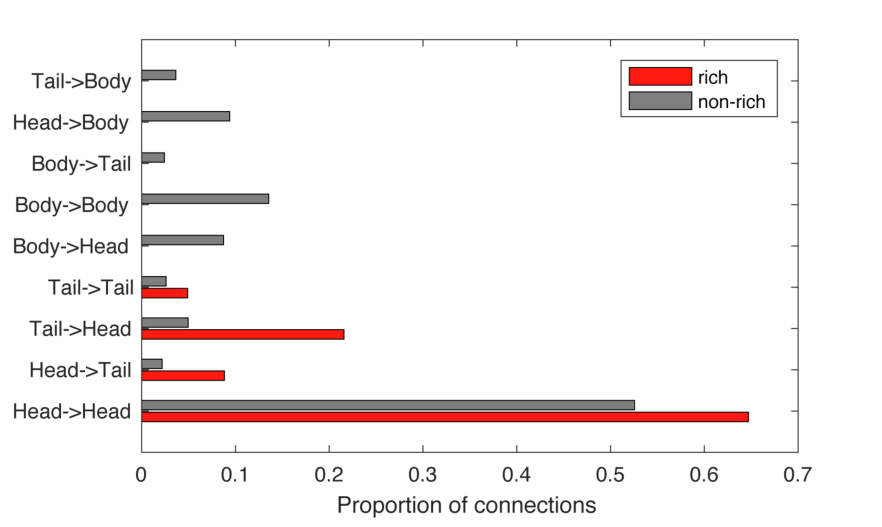
\includegraphics[width=1\textwidth]{Chapter2/Ch2S6fig.pdf}}
 \caption{{\bf Rich and non-rich connections in the \emph{C.elegans} connectome, categorized by the  anatomical location of the source and target neurons.}
   Hub-hub connections (`rich') are shown red, and all other connections (`non-rich', i.e., feeder and peripheral) are shown gray, where hubs are defined as neurons with degree, $k > 44$.
Anatomical locations are labeled as `head', `body', and `tail', and each connection is labeled according to its source and target neurons, listed on the vertical axis in the form `Source-Target'.
The plot shows that the increased separation distance between connected hubs relative to other types of connected neurons is driven by a relative increase in long-range connections between the head and tail.}
\label{fig:Ch2S6_Fig}
\end{figure}

\begin{figure}[h!]
  \centering{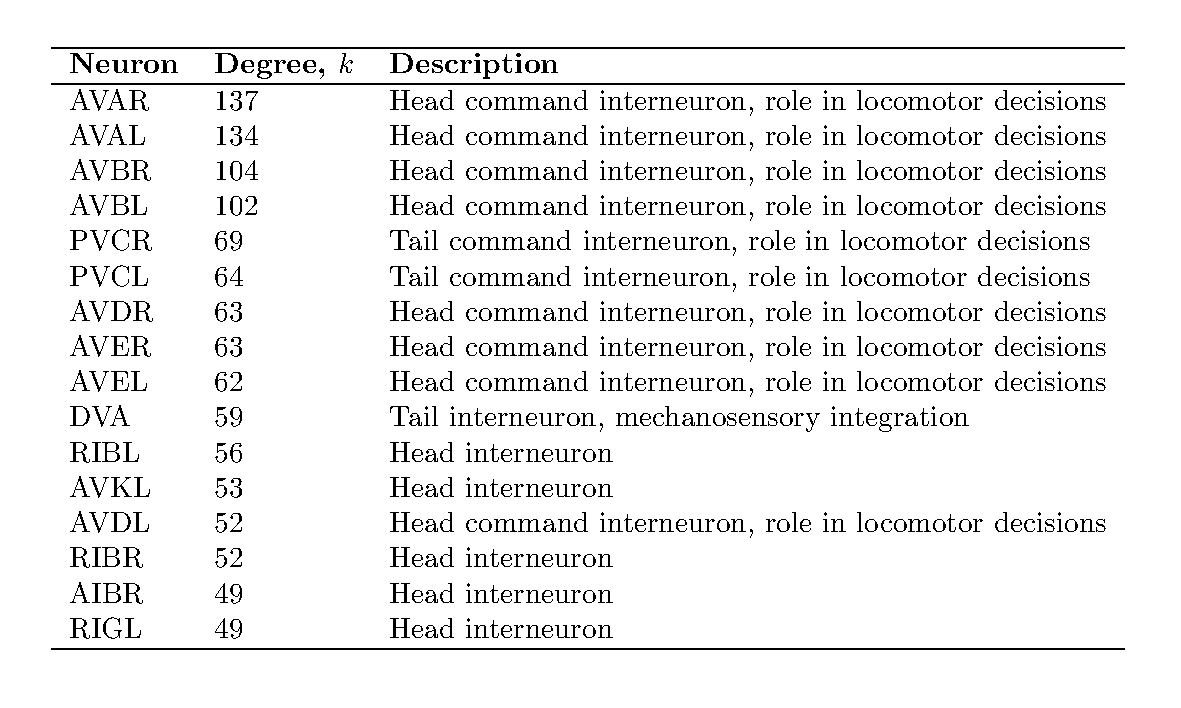
\includegraphics[width=1\textwidth]{Chapter2/Ch2S1Tab.pdf}}
   \caption{{\bf Hub neurons of the \textit{C.elegans} connectome.} Hubs are defined as neurons with degree $k > 44$. For each hub, we list (i) the neuron name, (ii) its degree, $k$, (iii) location (`head', `body', or `tail'), and function based on information presented in the wormatlas website \url{http://www.wormatlas.org/}.
Neurons are sorted (descending) by degree.}
\label{tab:HubList}
\end{figure}

\begin{figure}[h!]
  \centering{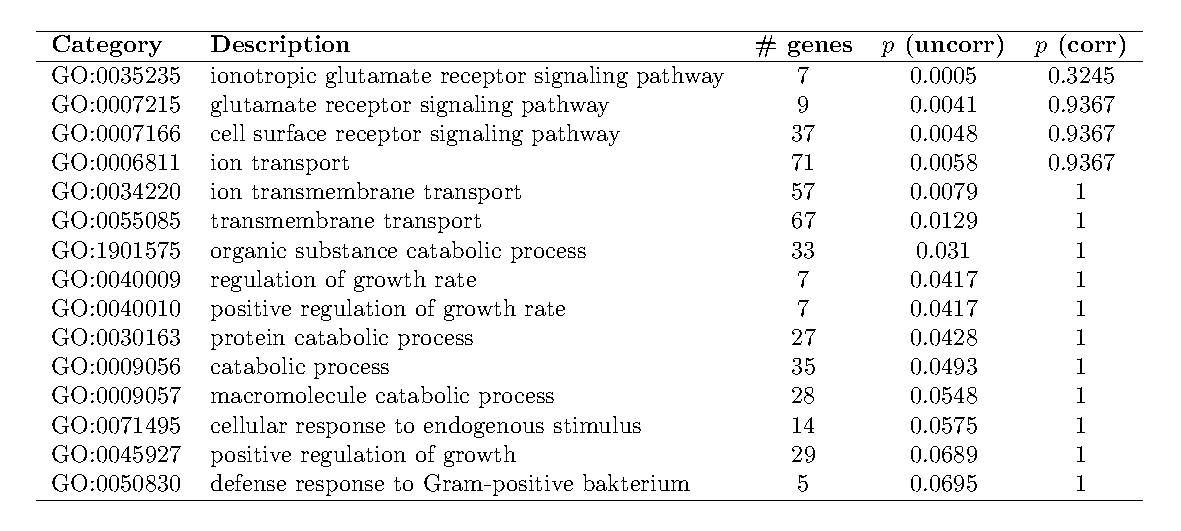
\includegraphics[width=1\textwidth]{Chapter2/Ch2S2Tab.pdf}}
   \caption{{\bf Enrichment results for connected \textit{vs} unconnected neurons.} Top 15 biological process GO categories enriched in genes with the highest mean increase in CGE for connected neurons compared to unconnected neurons.
Categories are sorted by $p$-value (ascending).}
\label{tab:enrichmentCON}
\end{figure}

\begin{figure}[h!]
  \centering{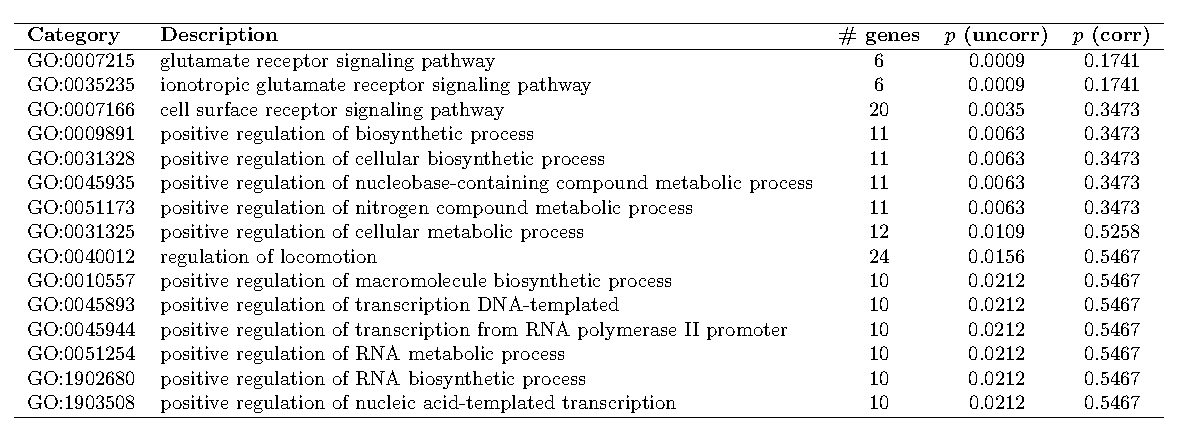
\includegraphics[width=1\textwidth]{Chapter2/Ch2S3Tab.pdf}}
   \caption{{\bf Enrichment results for links involving hubs.} Top 15 biological process GO categories enriched in genes with the highest increase in CGE for connections involving hub neurons (i.e., rich, feed-in and feed-out connections) compared to connections between nonhub neurons (i.e., in peripheral connections).
Categories are sorted by $p$-value (ascending).}
\label{tab:enrichmentRICH}
\end{figure}

\paragraph*{S1 File.}
\label{file:geneList}
{\bf Genes controbuting towards increased CGE.}
A list of genes that contributed towards the (i) increased CGE in connected compared to unconnected pairs of neurons, and (ii) increased CGE in rich and feeder compared to peripheral connections.

  %!TEX root = ../Thesis.tex
\chapter{Linking brain-wide gene expression and neuroimaging data}
\fancyhead[R]{\textit{Appendix B:~Linking brain-wide gene expression and neuroimaging data}}

\paragraph*{supplementary material S1}\mbox{}\\
\label{SItext1}

\textbf{Details on AHBA}\\
The AHBA microarray gene expression data consists of \num{3702} samples from six  neurotypical adult brains. Several hundred samples (mean $\pm$ standard deviation: $617 \pm 241$) were collected from cortical, subcortical, brainstem and cerebellar regions in each brain and profiled for genome-wide gene expression using custom Agilent $8\times60$K cDNA chip which consists of a standard Whole Human Genome Microarray Kit, $4\times44$K (Design ID: $014850$) and more than \num{18000} custom-generated probes created specifically for AHBA in order to increase the genetic coverage. Originally, \num{48171} of all \num{58692} probes were annotated to a gene, resulting in a set of \num{20787} unique genes with expression measures. In addition to gene expression data, the AHBA provides a binary indicator when the level of a given transcript exceeds background [as defined by the $t$-test -based criteria \citep{AHBAdoc}].
Each probe in the AHBA is associated with a numerical ID and a platform-specific label or name. If a probe is assigned to represent a unique gene it is also characterized with a range of gene-specific labels such as gene symbol and an entrez gene ID, a stable identifier for a gene generated by the Entrez Gene database at the National Center for Biotechnology Information (NCBI). If required, probe sequences can be accessed using the Allen Institute’s website application programming interface (see \nameref{SItext7}) while Agilent probe sequences can also be downloaded through the manufacturer's website (\url{https://earray.chem.agilent.com/earray/}). Probe sequences can also be found in the figshare repository \url{https://doi.org/10.6084/m9.figshare.6852911}. Note that the expression levels of a single gene can be measured using multiple probes that correspond to a different part of the gene sequence. In the AHBA, $93\%$ of all genes are annotated to more than one probe.

Probe-level data are available for each of \num{3702} tissue samples taken throughout the brain. Different brain regions were sampled across each of the six AHBA donors to maximize spatial coverage. Each tissue sample is associated with a numeric structure ID, name, and structure label (`cortex', `cerebellum', or `brainstem') in addition to the MRI voxel coordinates in native image space and MNI coordinates in standard space that can be used for matching samples to the stereotaxic space. The AHBA also provides RNA-seq data for a subset of tissue samples in two donor brains ($n=120$ each). It consists of expression values for more than \num{22000} genes presented in fragment count (number of reads matching a given gene) and TMP (Transcripts Per Kilobase Million - normalized read count with regards to read and transcript length) formats. RNA-seq method quantifies the transcription by directly sequencing each molecule in high-throughput manner, therefore providing a more precise measurement of levels of transcripts without the prior knowledge of the DNA sequence of interest \citep{Wang2009}.

Magnetic resonance images---T1-weighted, T2-weighted, T2-weighted gradient echo and FLAIR---were collected prior to dissection of each brain for anatomic visualization. Diffusion tensor images were collected for two brains (H0351\_2001 and H0351\_2002). Detailed information about image acquisition sequences is presented in a technical white paper \citep{AHBAdoc}.

\paragraph*{supplementary material S2}\mbox{}\\
\label{SItext2}

\textbf{Enrichment analysis} \\
\noindent Software: version 3.1.2 version of ErmineJ software \citep{Gillis2010};\\
Biological process GO annotations: obtained from GEMMA \citep{Zoubarev2012} as \\
\texttt{Generic\_human\_ncbiIds\_noParents.an.txt} downloaded on May 16, 2018. \\
Gene Ontology terms and definitions: obtained from \url{archive.geneontology.org/latest-termdb/go_daily-termdb.rdf-xml.gz} on May 16 2018.\\
The analyses were performed only on the biological process annotations. \\

\textbf{Intensity-based filtering}\\
To test if intensity-based filtering (where probes are filtered based on the binary indication of expression levels exceeding the background) targets any specific functional gene groups, we performed the gene score resampling (GSR) analysis. Avoiding the potential bias of overestimating the influence of genes that are represented with multiple probes scores for the GRS analysis were determined at gene (rather than probe) level by: (i) calculating the proportion of samples with expression values exceeding the background using the binary indicator provided by AHBA for each probe; (ii) if more than one probe was available for a gene, the probe with the highest proportion of samples exceeding the background was selected to represent that gene. As a result, each of the \num{20232} genes was assigned a score indicating the proportion of samples with expression levels exceeding the background. The analysis was performed focusing on genes with low scores in order to determine what functional gene groups are affected by intensity-based filtering. The mean score in a GO group was selected to summarize it, using full resampling with $10^{6}$ iterations. FDR-corrected $p$-values (across around \num{7000} GO categories) were used to summarize the effect. The significant GO categories (at $p_\mathrm{corr}<0.05$) include non brain-specific processes such as sensory perception, chemotaxis, cell killing, and immune response among others (a list of TOP $100$ GO categories is presented in supplementary file enrichmentExpression.csv). \\

\textbf{RNA-seq – microarray non-overlap}\\
The usage of RNA-seq expression measures for probe selection in microarray data is limited to genes that are present in both datasets. Given that $\sim13\%$ ($n=$\num{2623}) out of the  \num{20232} genes in the microarray data are not present in the RNA-seq dataset, we aimed to characterize the types of genes that do not have corresponding RNA-seq measures, and test if any brain-specific functional groups of genes are over-represented in this set as these genes would be excluded from the further analysis. If this is the case, then probe selection based on the correlation to RNA-seq data would not be an optimal solution due to the loss of relevant information. Overrepresentation analysis (ORA) was performed for each biological process GO category with $5$ to $100$ genes available taking the mean score in a GO group to summarize it. FDR-corrected $p$-values (across around \num{7000} GO categories) were used to summarize the effect. The significant GO categories (at $p_\mathrm{corr}<0.05$) include general processes such as septin assembly and organization as well as the negative regulation of RNA splicing among others (presented in supplementary file enrichmentExpression.csv) and are not related to brain-specific biological processes. \\

\textbf{Microarray and RNA-seq correlation}\\
In order for RNA-seq gene expression measures to provide a valid reference when selecting a probe, microarray and RNA-seq measures should be at least weakly correlated. Given that for a number of genes the maximum correlation between microarray and RNA-seq expression measures is very low, the probe selection based on such low correlations will be invalid. Therefore, we first exclude probes exhibiting a low correlation (taking a selected threshold, $\rho < 0.2$) to RNA-seq data resulting in the exclusion of \num{6725} genes. To evaluate the functional groups of genes that were removed, we performed an overrepresentation analysis (ORA). Avoiding the potential bias of overestimating the influence of genes that are represented with multiple probes, scores for the ORA analysis were determined at gene (rather than probe) level by: (i) calculating correlation between microarray and RNA-seq expression for each probe in two subjects; (ii) estimating the mean correlation for each probe across two subjects; (iii) if the maximum correlation value was lower than $0.2$, a gene was excluded and assigned an arbitrary value of $0$ to serve as a binary indicator of exclusion; otherwise a value of $1$ was assigned to represent a gene. As a result, each of \num{17609} genes were assigned a score indicating whether it was excluded due to low correlation to RNA-seq data. ORA was performed for each biological process GO category with $5$ to $100$ genes available taking the mean score in a GO group to summarize it. FDR-corrected $p$-values (across around \num{7000} GO categories) were used to summarize the effect. The significant (at $p_\mathrm{corr}<0.05$) GO categories include general processes such as immune response, DNA modification and regulation of transposition among others (in Supplementary File enrichmentExpression.csv).

To further verify that genes with higher correlations between microarray and RNA-seq were related to neuronal connectivity and communication related processes we performed gene score resampling analysis (GSR). Avoiding the potential bias of overestimating the influence of genes that are represented with multiple probes scores for the GSR analysis were determined at gene (rather than probe) level by: (i) calculating correlation between microarray and RNA-seq expression for each probe in two subjects; (ii) estimating the mean correlation for each probe across two subjects; (iii) if more than one probe was available for a gene, the maximum correlation value was selected to represent that gene. As a result, each of the \num{17609} genes that are present in both microarray and RNA-seq datasets was assigned a score indicating the maximum correlation between microarray and RNA-seq expression values across matching structures.

Focusing on genes with high scores in order to determine which functional gene groups are more likely to be correlated with RNA-seq expression values, we treated larger scores as indicative of the signal. Gene score resampling was performed for each biological process GO category with $5$ to $100$ genes available taking the mean score in a GO group to summarize it, using full resampling with $10^{6}$ iterations. FDR-corrected $p$-values (across around \num{7000} GO categories) were used to summarize the effect. The significant (at $p_\mathrm{corr}<0.05$) GO categories include brain-specific processed such as ensheathment of neurons, oligodendrocyte development, transmission of nerve impulse, glial cell development, central nervous system myelination, synaptic vesicle transport and action potential among others. Of the TOP $100$ significant GO categories, around $50\%$ are related to brain-specific processes (presented in supplementary file enrichmentExpression.csv; to emphasize the presence of processes that we have identified as brain-specific, we noted them in green).

\paragraph*{supplementary material S3}\mbox{}\\
\label{SItext3}

\textbf{Comments on differences between probe selection methods}\\
Two of the variance-based methods for probe selection—those based on choosing probes with high coefficient of variation or maximum variance—aim to select probes that vary most across the brain. This approach is based on the logic that investigators are often interested in genes that show variation in expression across brain regions. However, probes with higher variance tend to have lower mean intensity because a lower hybridization leads higher signal variability \citep{Quackenbush2002a}. Indeed, we find a negative relationship between expression variance and mean intensity across probes with expression values exceeding the background (average probe intensity $> 3$; $\rho = -0.44$, $p < 0.001$, Spearman’s rank correlation, see Figure \ref{fig:Ch4Sfig4}).

Choosing a probe based on the highest loading on the first PC aims to select the probe with the most representative expression pattern based on the probe-to-probe variance-covariance matrix. If the probes are not correlated, the first PC will not be representative. Correlations between probes selected using variance-based and consistency/intensity-based approaches are lower than those obtained through random selection. This suggests that variance and intensity/consistency-based approaches favour probes with more different expression measures, meaning that probes with the highest variance would tend on average to be less consistent than randomly selected probes and vice versa (Figure \ref{fig:Ch4Fig4}A, for the comparison between probe selection methods after QC filtering is applied see Figure \ref{fig:Ch4Sfig1}).

The most popular approach is to summarize gene expression as a mean of all available probes (see Table \ref{Table2}). This method shows high similarity to all other methods. Given that probes can measure different parts of the same gene with different sensitivity, expression measures quantified using different probes are likely not to be equivalent. In this case summarising expression of the gene by calculating the mean of all available probes is likely to reduce this variability.
Consistency-based probe selection selects probes with the most consistent regional expression patterns across the six brains in the AHBA, using a measure called differential stability (DS), first introduced in  \citet{Hawrylycz2015}. The first analysis of the AHBA data indicated that regional variation in expression levels across anatomical structures was strongly correlated between different brains, thus between-region variation in expression should dominate between-subject variance. Choosing a probe with consistent regional variation assumes that this variation is real, and that any between-subject variance is noise. Such an approach is justifiable in analyses where investigation of regional variations in gene expression are the goal. While high DS values are relatively easy to interpret, low DS values could reflect at least three different scenarios: (i) low signal-to-noise ratio across samples; (ii) the presence of true and significant inter-subject variability; (iii) relatively spatially homogeneous patterns of expression within each donor brain. These options should be considered when implementing the DS metric.
When combining data across the donors, the same probe should be chosen to represent gene expression across the six donor brains. This is necessary in order to ensure that the probes used to measure the expression levels of a particular gene hybridize to the same part of that gene.

\paragraph*{supplementary material S4}\mbox{}\\
\label{SItext4}

\textbf{Information regarding sample assignment}\\
The data provided with this manuscript consists of four region $\times$ gene matrices for left cortical regions. Here we focus only on the left hemisphere as right hemisphere samples were only collected from two of the six AHBA donor brains. We focus only on cortex because major gene expression differences between cortex and subcortex mean that collapsing data from both requires careful consideration regarding appropriate normalization strategies. These decisions are contingent on one’s research questions. Region $\times$ gene matrices containing data from both hemispheres and including sub-cortical regions can be generated using the processing pipeline provided in the github repository \url{https://github.com/BMHLab/AHBAprocessing}. Below we provide some summary information regarding the sample assignment to the left cortical region in each parcellation applying $2\,mm$ distance threshold:

\begin{figure}[h!]
  \centering
    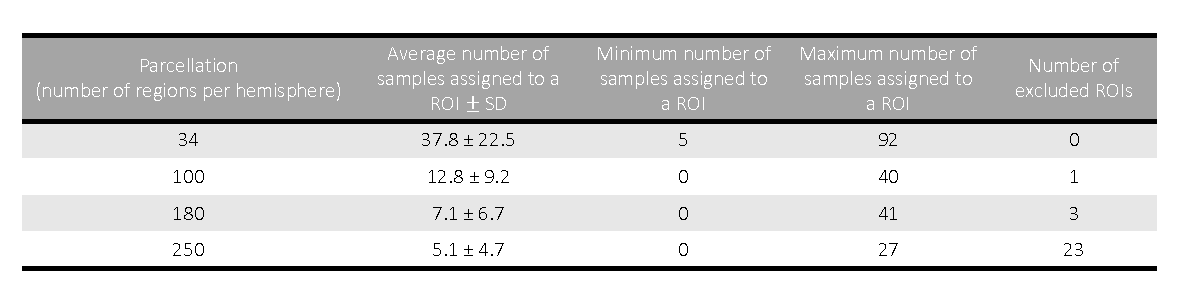
\includegraphics[width=1\textwidth]{Chapter4/TableS4.pdf}
\label{TableS4}
\end{figure}

\paragraph*{supplementary material S5}\mbox{}\\
\label{SItext5}

\textbf{Evaluating distances between samples}\\
All distances between samples were calculated on a set of samples that were mapped onto individual parcellations applying a $2\,$mm distance threshold as described in Step $4$. Voxel coordinates provided by the AHBA that were used to map samples to subject-specific parcellations are derived from images in subject space and could not be combined to estimate distances between samples from different subjects. Therefore, for both Euclidean distances and distances within cortical surfaces we used MNI coordinates provided by the AHBA for each region to estimate the pairwise distances between them given that MNI coordinates are derived in the same space for all subjects.

\textbf{Euclidean distances} were calculated using the function \texttt{pdist2} in MATLAB 2016b\footnote{MATLAB is a product of Mathworks}.

\textbf{Distances within cortical volume} were calculated using an HCPMMP1 \citep{Glasser2016} parcellation in the MNI space (downloaded from \url{https://neurovault.org/collections/1549/}, file \texttt{MMP\_in\_MNI\_corr.nii})  by: i) changing the strides of the image from $[-1 3 -2]$ to $[-1 2 3]$ in order to change the image orientation; ii) rendering the brain parcellation in MNI space as a 3D matrix; ii) converting the original MNI sample coordinates to voxel-based coordinates that correspond to the parcellation loaded in a 3D matrix format; iv) finding the closest coordinate in the parcellation for each sample and mapping a sample to that location; v) rendering the parcellation as a graph with each voxel representing a node; vi) implementing Dijkstra’s algorithm \citep{Dijkstra1959} to calculate the closest distances between samples within the GM volume using \texttt{shortestpath} function in MATLAB. Distances between pairs of regions were calculated as an average of distances between samples within them.

\textbf{Distance on the cortical surface} were calculated using annotation files for each parcellation and the spherical representation of the cortical surface by: i) identifying vertices that correspond to a particular region on the sphere and calculating the mean of their coordinates to obtain a centroid value; ii) mapping centroid coordinates to the cortical surface representation; iii) calculating the distances between each pair of regions using the \texttt{toolbox\_fast\_marching} toolbox in MATLAB.

\paragraph*{supplementary material S6}\mbox{}\\
\label{SItext6}

\textbf{Spatial relationship between CGE and distance}\\
Figure \ref{fig:Ch4Sfig9}B shows the relationship between CGE and separation distance for three different types of regional pairs: (i) intra-cortical region pairs, which show relatively high CGE at all distances (light grey); (ii) intra-subcortical region pairs, which show a linearly decreasing relationship at short distances (dark grey); and (iii) cortical-subcortical region pairs, which demonstrate mostly negative CGE at all distances (peach). This variability precludes simple removal of a global trend as in \citep{Fulcher2016} and suggests a separate correction should be applied for each class of connection. Figure \ref{fig:Ch4Sfig9}C shows the result of removing the mean CGE at each equiprobable distance bin separately for each connection class. Even after this correction, intracortical CGE values appear to be underestimated while cortico-subcortical are overestimated. Another method for addressing the inherent differences between cortical and subcortical gene expression profiles is to normalize the expression data separately for these two anatomical divisions [e.g., \citet{Anderson2018}]. With this approach, expression values are scaled relative to other values within just the cortex, or within just the subcortex. Division-specific normalization allows a gene to score highly if its expression in the subcortex is high relative to other subcortical regions, even if its expression relative to the cortex may be low (and vice-versa), at the expense of distorting the magnitude relationships between cortical and subcortical values. With this approach, the negative correlation between cortical and subcortical regions is reduced with some region pairs demonstrating relatively similar gene expression profiles (Figure \ref{fig:Ch4Sfig9}D). As presented in Figure \ref{fig:Ch4Sfig9}E, the relationship between CGE and separation distance is now more qualitatively similar for all three groups and can be corrected using simple mean subtraction across distance bins (Figure \ref{fig:Ch4Sfig9}F).

\paragraph*{supplementary material S7}\mbox{}\\
\label{SItext7}

\textbf{API: probe sequences} for the first \num{10000} rows.\\
\url{http://api.brain-map.org/api/v2/data/query.xml?criteria=model::Probe,rma::criteria,products[id$eq2],rma::include,gene,predicted_sequence,rma::options[only$eq%27probes.name,probes.type,probes.ncbi_accession_number,probes.gi,genes.entrez_id,genes.acronym,sequences.sequence_length,sequences.sequence_data%27],[num_rows$eq10000][start_row$eq0]}

\newpage

\begin{figure}[h!]
  \centering
    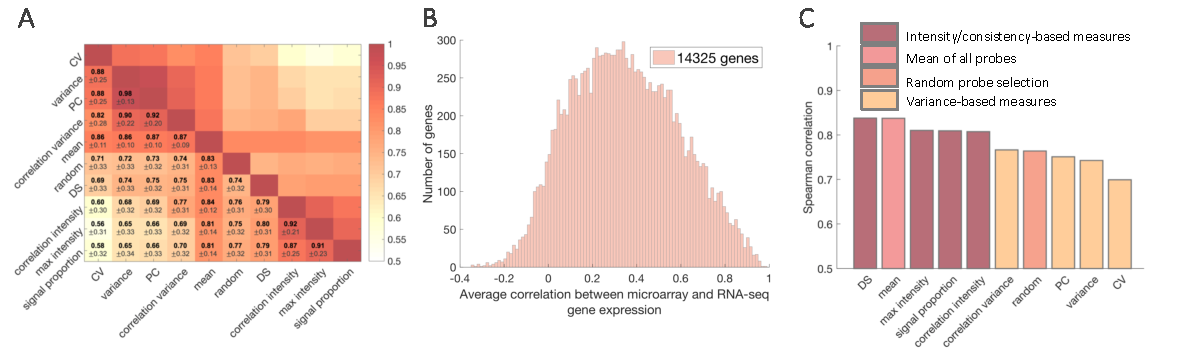
\includegraphics[width=1\textwidth]{Chapter4/FigureS1.pdf}
\caption{\textbf{Average correlation between summary expression scores for genes annotated to multiple probes, where a single representative probe is chosen based on different criteria after intensity-based filtering (IBF).}
A) Average correlation between summary expression scores for genes annotated to multiple probes, where a single representative probe is chosen based on different criteria: CV, variance, PC, signal proportion, DS, correlation variance, correlation intensity, mean (see Table \ref{Table2}) or selecting a representative probe at random (correlation values averaged over $100$ runs). The average correlation is computed over \num{11190} genes with multiple probe annotations after intensity-based filtering. B) The distribution of Spearman correlation coefficients between microarray and RNA-seq expression data for genes that are present in both datasets. When multiple probes for a gene were available, the maximum correlation value between probes was selected. IBF increases the average correlation between microarray and RNA-seq gene expression measures relative to not using IBF, Wilcoxon rank-sum test, $p=1.1 \times 10^{-49}$. C) Average correlation between probes selected using RNA-seq expression (by selecting the probe that is correlated to the RNA-seq data the most) and other methods (ordered by decreasing values, based on \num{7950} genes that (i) were present in both microarray and RNA-seq datasets; (ii) were correlated to RNA-seq in excess of a threshold value ($\rho > 0.2$, Spearman rank correlation) to ensure that RNA-seq based probe selection provides a meaningful estimate of the microarray measures; (iii) had more than one probe available after intensity-based filtering). }
\label{fig:Ch4Sfig1}
\end{figure}

\begin{figure}[h!]
  \centering
    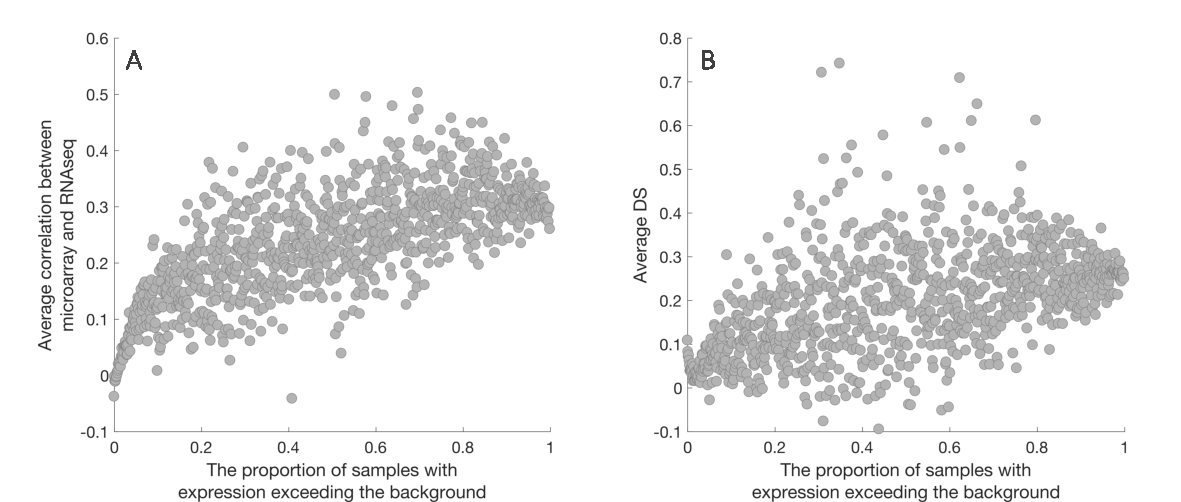
\includegraphics[width=1\textwidth]{Chapter4/FigureS2.pdf}
\caption{\textbf{The effect of intensity based filtering.}
The relationship between the proportion of samples with expression measures exceeding the background and A) the average correlation between microarray and RNA-seq expression measures at the probe level (Spearman’s $\rho = 0.3$, $p<0.001$); B) the average differential stability (DS) for each gene (Spearman’s $\rho = 0.33$, $p<0.001$). DS measures were calculated based on the scaled robust sigmoid normalized data (see Eq.\ref{eqn:eq2}) within the regions of the left cortex. Correlation and differential stability values are averaged within 1000 bins to aid visualization.}
\label{fig:Ch4Sfig2}
\end{figure}

\begin{figure}[h!]
  \centering
    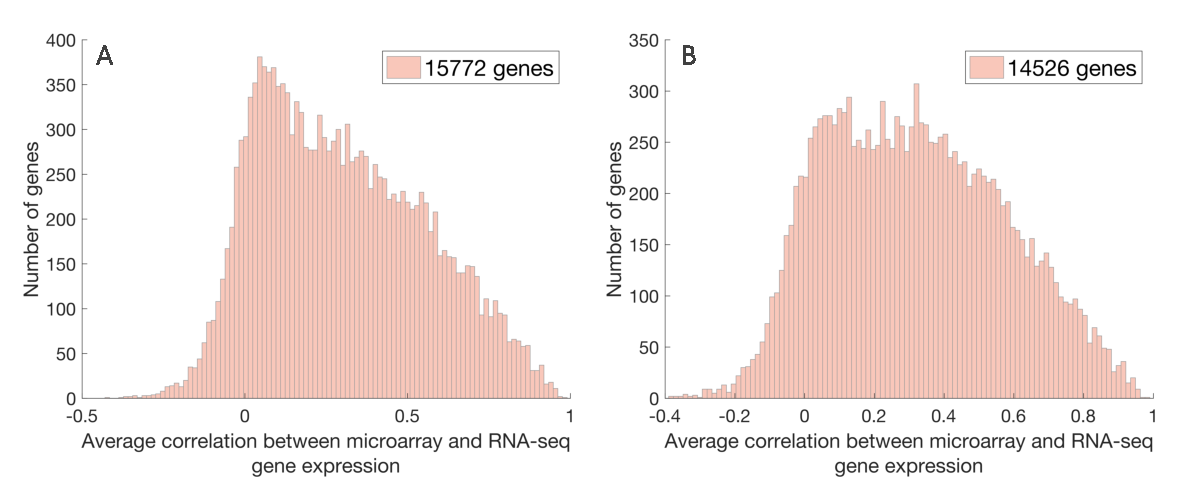
\includegraphics[width=1\textwidth]{Chapter4/FigureS3.pdf}
\caption{\textbf{Correlation to RNA-seq expression measures and gene expression measures obtained following variance-based filtering of probes.}
In variance-based filtering probes with the lowest variance are to be excluded. A probe was excluded if it was consistently classified within the $50\%$ of the  lowest variance probes in all six brains. This figure shows the distribution of Spearman correlation values between microarray and RNA-seq expression data for genes that are present in both datasets when the variance-based filtering is applied to $\log_2$-transformed data (A) and non-transformed data (B). We use RNA-seq data as a gold standard to verify microarray filtering results. When multiple probes for a gene were available, the probe with the maximum correlation value was selected. Variance-based filtering on $\log_2$-transformed data decreases the correlation between microarray and RNA-seq expression measures compared to the data prior to filtering (Wilcoxon rank-sum test, $p = 10^{-5}$). Variance-based filtering on non-transformed data increases the mean correlation (Wilcoxon rank-sum test, $p = 0.008$), but the increase is not as large as when using intensity-based filtering (see Figure \ref{fig:Ch4Sfig1}).}
\label{fig:Ch4Sfig3}
\end{figure}

\begin{figure}[h!]
  \centering
    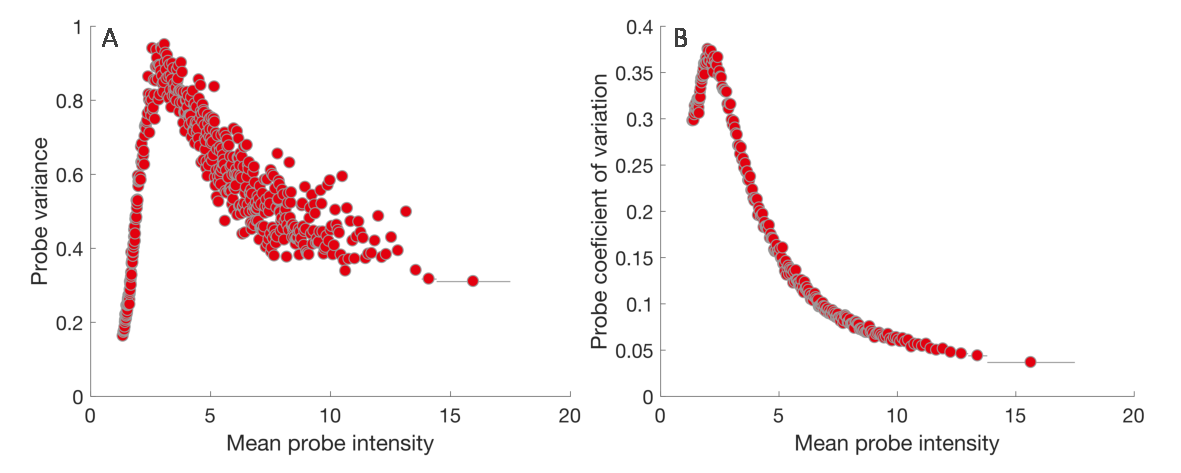
\includegraphics[width=1\textwidth]{Chapter4/FigureS4.pdf}
\caption{\textbf{The relationship between average probe intensity, variance, and coefficient of variation.}
The relationship between average probe intensity and A) variance, and B) coefficient of variation in $500$ and $250$ equiprobable intensity bins respectively, shown as a circle (bin centers) and a horizontal line (bin extent). The relationship between probe intensity and variance is positive for low intensity probes (intensity$<3$); for higher intensity probes increasing intensity results in decreasing variance. The same trend is evident for the relationship between coefficient of variation and intensity.}
\label{fig:Ch4Sfig4}
\end{figure}

\begin{figure}[h!]
  \centering
    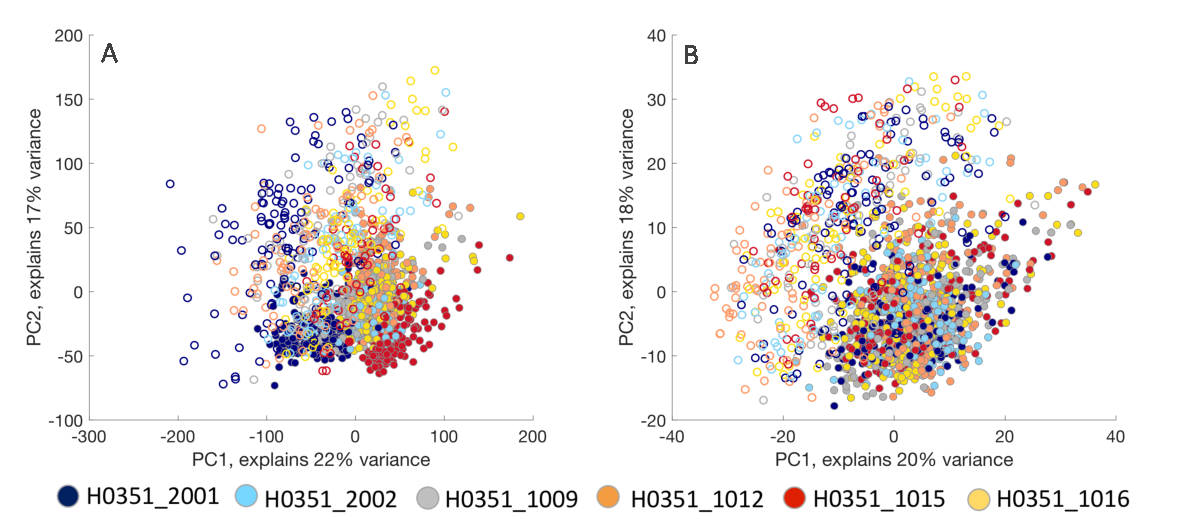
\includegraphics[width=1\textwidth]{Chapter4/FigureS5.pdf}
\caption{\textbf{Inter-individual differences in gene expression and the effect of normalization in the whole brain.}
A) Original gene expression data for cortical and subcortical samples in principal component space. Data from different donors are represented in different colours. Samples from different subjects occupy different parts of the low-dimensional gene expression space. B) gene expression data in principal component space normalized using scaled robust sigmoid (SRS). After normalization samples no longer segregate by donor and show a more clear separation between cortex and subcortex. Filled and closed markers denote cortical and subcortical regions, respectively.}
\label{fig:Ch4Sfig5}
\end{figure}

\begin{figure}[h!]
  \centering
    \includegraphics[width=1\textwidth]{Chapter4/FigureS6.pdf}
\caption{\textbf{A schematic representation of cross-gene and cross-sample normalization.} Within-sample cross-gene normalization estimates the relative expression level of all available genes within a given sample (grey row). Within-gene cross sample normalization estimates the relative expression of a particular gene across all available samples (red column).}
\label{fig:Ch4Sfig6}
\end{figure}

\begin{figure}[h!]
  \centering
    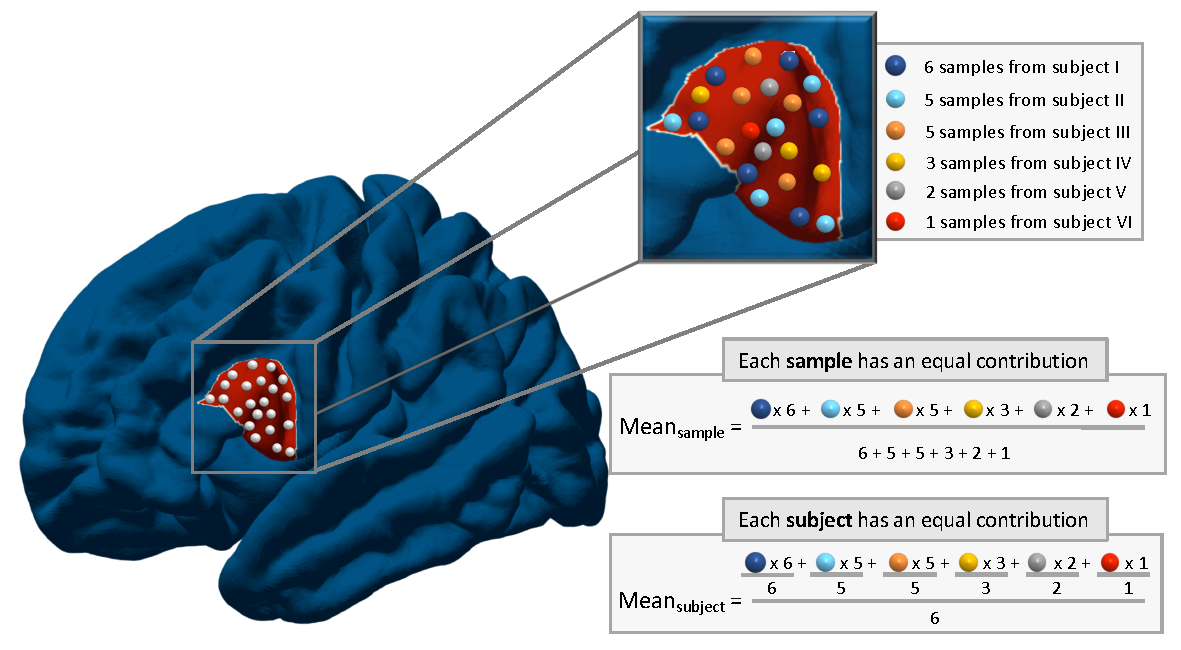
\includegraphics[width=1\textwidth]{Chapter4/FigureS7.pdf}
\caption{\textbf{Two alternative ways of averaging expression values within the region of interest. }
Each region of interest might contain a different number of samples from each subject. For example, the presented region has $6$ samples from subject I, $5$ samples from subjects II and III, $3$ samples from subject IV and only $2$ and $1$ samples from subjects V and VI respectively. One way of calculating the mean is to take the average of all samples, such that each sample makes an equal contribution to the overall expression value ($\mathrm{Mean_{sample}}$). An alternative is to average the samples from each donor first, and then take a second-order average across donors ($\mathrm{Mean_{subject}}$). The latter ensures that each subject makes an equal contribution to the summary expression value. The former might be influenced by donors with more samples in a given region. The choice of inter-subject averaging does not significantly impact the statistics in the reported study. As an example, for the cortical parcellation containing 180 regions per hemisphere, we compare data using both sample and subject-level averaging. The mean correlation between resulting regional expression vectors (for each region across all genes) is $0.97$ ($SD = 0.04$). The lowest correlation (outlier) is $0.76$ for one region, which contains samples from three subjects [S1($n=2$), S2($n=6$), S5($n=1$)]. In this region, S2 dominates the mean if the average across samples is taken. The mean correlation between gene expression measures (for each gene across regions) is also $0.97$ ($SD = 0.01$) with no obvious outliers. These findings suggest that different averaging approaches are likely to have a minor effect on study findings at a global level, but could affect regionally-focused analyses; particularly regions with an uneven distribution of samples across donors.}
\label{fig:Ch4Sfig7}
\end{figure}

\begin{figure}[h!]
  \centering
    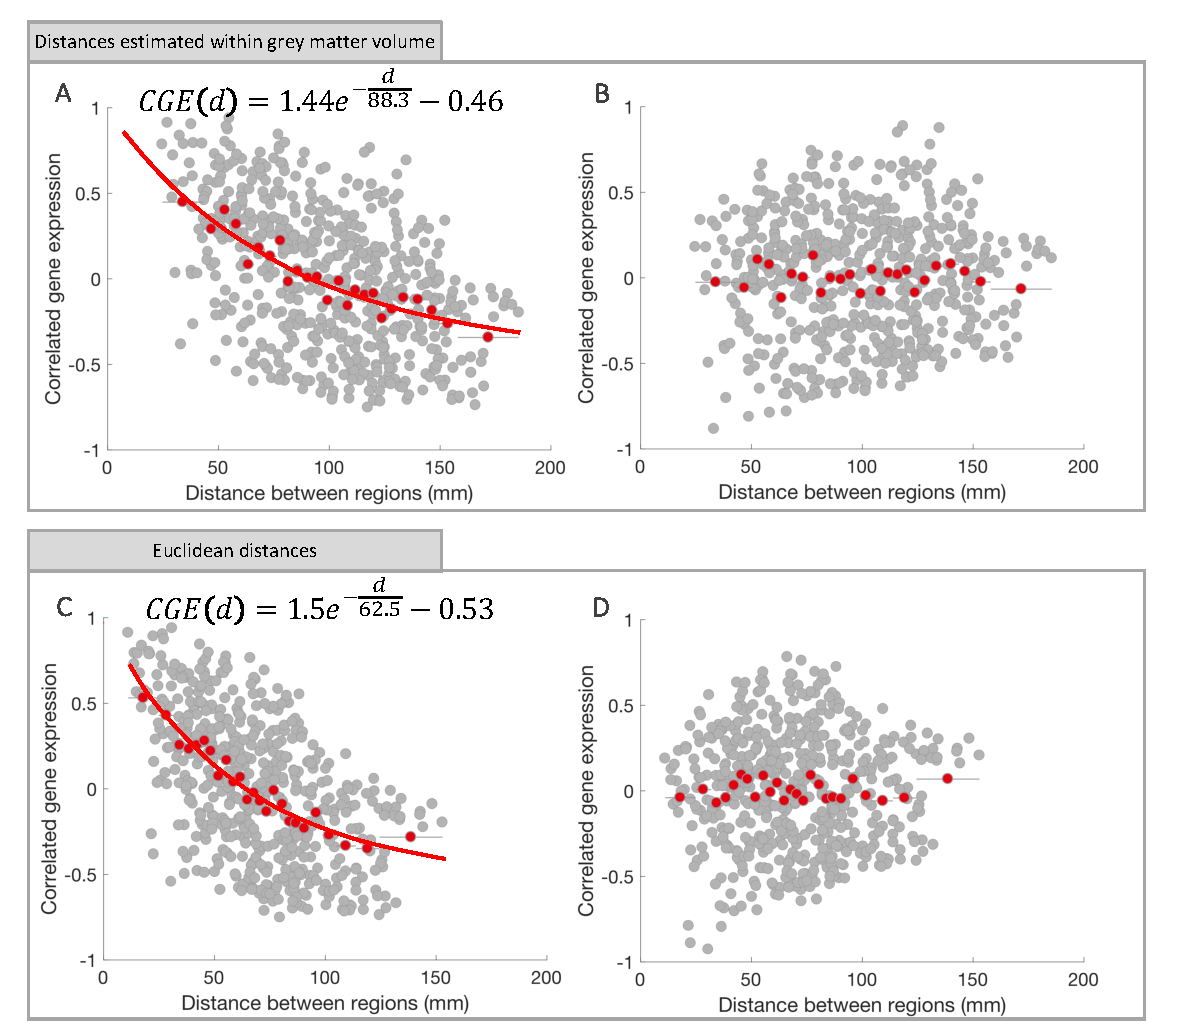
\includegraphics[width=1\textwidth]{Chapter4/FigureS8.pdf}
\caption{\textbf{The relationship between CGE and inter-regional distance estimated within grey matter volume and as Euclidean distance.}
Top: the relationship between CGE and distance when the distance between regions calculated within grey matter volume. Bottom: the relationship between CGE and distance when the distance between regions calculated as Euclidean distance. A,C) CGE as a function of separation distance where CGE between pairs of regions are represented in grey dots and red dots represent the mean value in $25$ equiprobable distance bins; The red line represents an exponential fit. A) $CGE(d) = 1.44e^{-d/88.3}-0.46$; C) $CGE(d)=1.5e^{-d/62.5}-0.53$.
B,D) Residuals after removing the exponential trend in each case;
CGE calculated using all \num{10027} genes (after intensity-based filtering and probe selection based on correlation to RNA-seq data). }
\label{fig:Ch4Sfig8}
\end{figure}

\begin{figure}[h!]
  \centering
    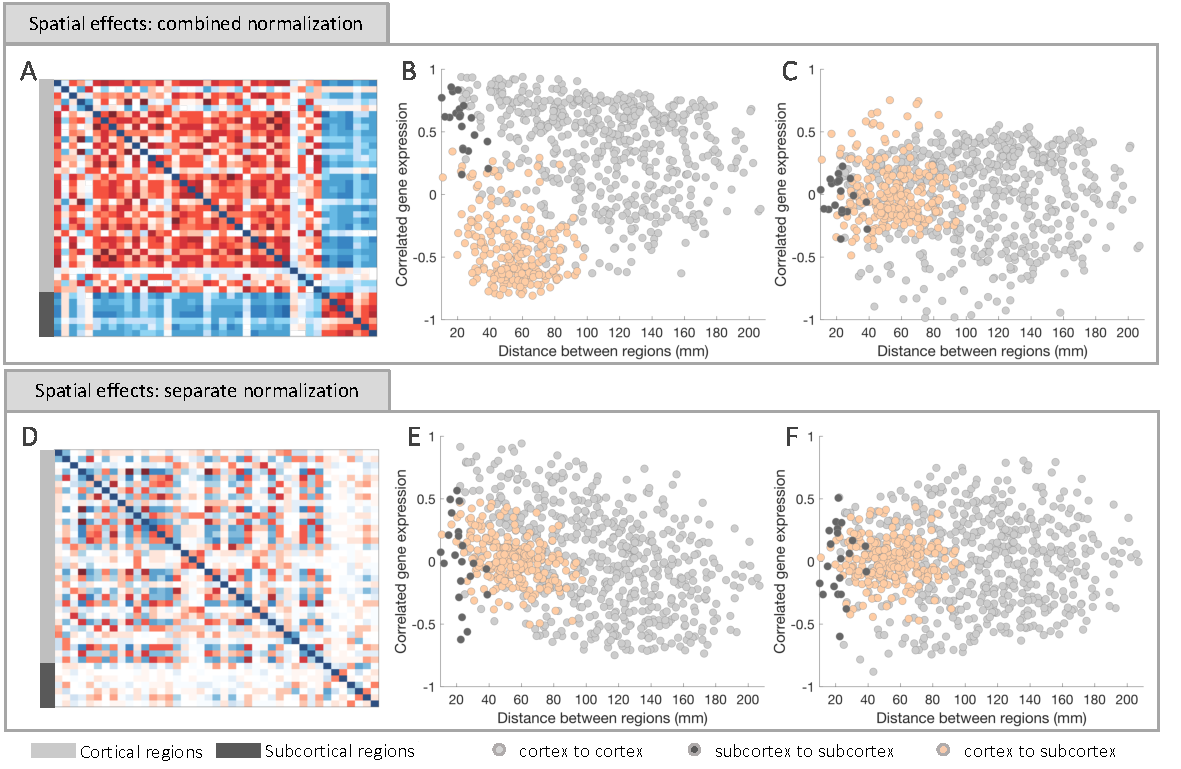
\includegraphics[width=1\textwidth]{Chapter4/FigureS9.pdf}
\caption{\textbf{The relationship between CGE and inter-regional distance for cortical and subcortical regions.}
Top row: A) Matrix of CGE values for the left hemisphere, including both cortical and subcortical regions, in which expression values have been normalized for both cortical and subcortical regions together; B) CGE as a function of separation distance where CGE between different subsets of regions are represented in different colours: within cortex --- light grey, within subcortex --- dark grey, between cortex and subcortex --- peach; C) CGE residuals after removing the spatial effect for each subset of regions separately by subtracting the average of each bin, where different colours represent subsets of connections as above. D) Matrix of CGE values for the left hemisphere, including both cortical and subcortical regions, in which expression values have been normalized separately for cortical and subcortical regions; E) CGE as a function of separation distance, where normalization has been performed on cortical and subcortical regions separately. Different colours represent subsets of connections as above; F) CGE residuals after removing the spatial effect for each subset of regions (when normalization performed on cortical and subcortical regions separately) by subtracting the average of each bin where different colours represent subsets of connections as above. Distances between cortical regions were evaluated on the cortical surface while distances between subcortical regions as well as between cortical and subcortical regions estimated as Euclidean.}
\label{fig:Ch4Sfig9}
\end{figure}

\begin{figure}[h!]
  \centering
    \includegraphics[width=1.1\textwidth]{Chapter4/FigureS10.pdf}
\caption{\textbf{The relationship between CGE and inter-regional distance on the cortical surface for high and low resolution parcellations using a full set of genes and a set of only highest DS genes.}
The relationship between CGE and inter-regional distance for different resolution cortical parcellations and different sets of genes. Top row: low resolution Desikan-Killany parcellation \citep{Desikan2006} ($34$ regions). Bottom row: high resolution HCPMMP1 \citep{Glasser2016} parcellation ($180$ regions). First column: CGE calculated using only $10\%$ of highest DS genes that are most consistently expressed across subjects and regions. Second column: CGE calculated using all \num{10027} genes. The relationship between CGE and inter-regional distance also depends on the subset of genes chosen for the calculation, such that high DS genes show a stronger association with inter-regional distance. This effect is more pronounced in the higher resolution parcellation.}
\label{fig:Ch4Sfig10}
\end{figure}

  %!TEX root = ../Thesis.tex
\chapter{Genetic markers of hub connectivity in the human brain}
\label{appendixC}
\fancyhead[R]{\textit{Appendix C:~Genetic markers of hub connectivity in the human brain}}

\section{Processing gene expression data}
\label{app:AppendixCh5_1}

Microarray gene expression and all the accompanying metadata were downloaded from the \url{http://human.brain-map.org/static/download}. The raw data consisted of \num{58692} probes quantifying the expression of \num{20737} genes in \num{3702} tissue samples in six neurotypical adult brains. The pre-processing procedures applied to the data are outlined below and the choices detailed in \mbox{\citep{Arnatkeviciute2019}}. Data used for the analyses can be found in the figshare repository: \url{https://figshare.com/s/441295fe494375aa0c13}.

\begin{enumerate}\addtocounter{enumii}{5}% This cannot be more than 25
      \item Probe-to-gene annotations were updated Re-Annotator software toolbox \citep{Arloth2015} resulting in the selection of \num{45821} probes corresponding to the total of \num{20232} genes.
      \item Tissue samples annotated to the brainstem and cerebellum were removed.
      \item Intensity based filtering was applied in order to exclude probes that do not exceed the background noise in more than 50\% of cortical and subcortical samples excluding \num{13844} probes corresponding to \num{4486} unique genes.
      \item If more than one probe was available for a gene, a representative probe was selected based on the correlation to RNA sequencing data \citep{Miller2014a} by applying several additional thresholding criteria:
      \begin{enumerate}
      \item genes that did not have the corresponding RNA-seq measures were removed;
      \item probes that demonstrated a low correlation to RNA-seq data (Spearman $\rho<0.2$) were removed;
	  \item a representative probe for a gene was selected based on the highest correlation to the RNA-seq data in the corresponding samples.
      \end{enumerate}
      \item Gene expression samples were assigned to the regions-of-interest by generating donor-specific grey matter parcellations and assigning samples located within $2$ mm of the parcellation voxels. To increase the assignment accuracy, samples were first divided into four separate groups based on their location: hemisphere (left/right) and structure assignment (cortex/subcortex), so samples listed as coming from the left cortical hemisphere as per AHBA ontology are only mapped to left cortical voxels of the parcellation. Applying $2$ mm distance threshold almost 90\% of all cortical and subcortical samples were assigned to a non-zero voxel of the parcellation.
      \item Samples assigned to the subcortical regions as well as samples assigned to the right hemisphere were removed.
      \item To account for inter-individual differences in gene expression between the donor brains, gene expression measures within a given brain (left cortical samples) were normalised by applying a scaled robust sigmoid normalisation \citep{Arnatkeviciute2019} in two separate steps:
      \begin{enumerate}
      \item For every sample across all genes to quantify the relative expression of every gene within each sample;
      \item For every gene across all samples to evaluate the relative expression of each gene across regions.
      \end{enumerate}
      \item The resulting normalised expression measures assigned to the same region in the parcellation were averaged and aggregated into a region by gene matrix consisting of expression measures for \num{10027} genes over 180 and 250 cortical regions respectively.
      \item Distances between those regions were estimated on the cortical surface (pial) using the annotation files for each parcellation, the spherical and the fsaverage representation of the cortical surface. First, all the vertices that correspond to a particular region in the spherical representation were identified and their centroid coordinates were calculated. Then the centroid coordinates were mapped to the fsaverage cortical surface and the distances between each pair of regions were calculated using the toolbox \texttt{fast\_marching\_toolbox} in MATLAB.
\end{enumerate}

\newpage
\section{Robustness to data processing decisions}
\label{app:AppendixCh5_2}

In this section we show robustness checks for data processing decisions. To evaluate how sensitive our findings are to the parcellation and connection density choices, here we present a set of the main findings using two different parcellations containing i) 360 functionally defined (f360) and ii) 500 randomly defined (r500) regions at different connectome densities. If not stated otherwise, the top row (panels A-C) contains results replicated using f360 parcellation and the bottom row (panels D-F) -- r500 parcellation. In all cases connectomes maintain the topological (Figure \ref{fig:Ch5SFig1}) and weighted (Figure \ref{fig:Ch5SFig2}) rich-club organisation with a slightly increasing consistency of the effect for the topological rich-club organisation at higher connectome densities (compare Figure \ref{fig:Ch5SFig1} A and C; D and F).

\begin{figure}[h!]
\begin{center}
\includegraphics[width=1\textwidth]{Chapter5/SFigure1.pdf}% This is a *.eps file
\end{center}
\caption{\textbf{Topological rich-club.}
Topological rich-club results reproduced using: top row -- 360 region parcellation at $15\%$ (A), $20\%$ (B), $25\%$ (C) connectome density; bottom row -- 500 region parcellation at $10\%$ (D), $15\%$ (E), $20\%$ (F) connectome density. In each plot top: The degree distribution of the group-level connectome. Bottom: Normalised topological rich-club coefficient ($\Phi_{norm}$); $\Phi_{norm}>1$ indicates that hubs are more densely interconnected than expected by chance; circles indicate values that are significantly higher than an ensemble of 1000 degree-matched null networks ($p<0.05$).}
\label{fig:Ch5SFig1}
\end{figure}

\begin{figure}[h!]
\begin{center}
\includegraphics[width=1\textwidth]{Chapter5/SFigure2.pdf}% This is a *.eps file
\end{center}
\caption{\textbf{Weighted rich-club.}
Weighted rich-club results reproduced using: top row -- 360 region parcellation at $15\%$ (A), $20\%$ (B), $25\%$ (C) connectome density; bottom row -- 500 region parcellation at $10\%$ (D), $15\%$ (E), $20\%$ (F) connectome density. In each plot top: The degree distribution of the group-level connectome. Bottom: Normalised weighted rich-club coefficient ($\Phi_{norm}$); $\Phi_{norm}>1$ indicates that connections between hubs are stronger than expected by chance; circles indicate values that are significantly higher than an ensemble of 1000 null networks ($p<0.05$) where the connections weights were randomised while preserving the topology. }
\label{fig:Ch5SFig2}
\end{figure}

\clearpage
Heritability estimates remain significantly increased for rich links in both f360 and r500 parcellations at all densities (Figure \ref{fig:Ch5SFig3}). Overall heritability estimates within the lower density connectomes were slightly higher compared to the denser ones (the dotted line shifts down along the columns). Connectomes defined based on the r500 parcellation demonstrate marginally lower heritability that might be related to the lower connectome density ($15-25\%$ \textit{vs} $10-20\%$). A little higher heritability for the rich links with a more consistent increase at the highest degrees were obtained using a f360 parcellation likely due to a slightly higher number of nodes at the very end of the degree distribution.

\begin{figure}[h!]
\begin{center}
\includegraphics[width=1\textwidth]{Chapter5/SFigure3.pdf}% This is a *.eps file
\end{center}
\caption{\textbf{Heritability.}
Mean edge heritability results reproduced using: top row -- 360 region parcellation at $15\%$ (A), $20\%$ (B), $25\%$ (C) connectome density; bottom row -- 500 region parcellation at $10\%$ (D), $15\%$ (E), $20\%$ (F) connectome density. In each plot top: The degree distribution of the group-level connectome. Bottom: Mean edge heritability for `rich' (hub -- hub), `feeder' (hub -- nonhub), `peripheral' (nonhub -- nonhub) connections as a function of degree threshold, \textit{k} used to define hubs. The mean heritability across all network links shown as a dotted black line. Circles indicate a statistically significant increase in heritability in a given link type compared to the rest of the network (one-sided Welch's $t$-test, $p < 0.05$).}
\label{fig:Ch5SFig3}
\end{figure}

\clearpage
Correlated gene expression remains significantly increased for rich links in both parcellations across a range of degree thresholds (Figure \ref{fig:Ch5SFig4}). Within the functionally defined parcellation, the increase in CGE is more pronounced at the lower connectome densities which might be related to the potentially increased number of false positive connections at higher densities. Comparable results for rich links are evident within the r500 parcellation with feeder links demonstrating a more significant increase in CGE compared to only a marginal effect in f360 parcellation.

\begin{figure}[h!]
\begin{center}
\includegraphics[width=1\textwidth]{Chapter5/SFigure4.pdf}% This is a *.eps file
\end{center}
\caption{\textbf{Transcriptional coupling.}
Mean correlated gene expression results reproduced using: top row -- 360 region parcellation at $15\%$ (A), $20\%$ (B), $25\%$ (C) connectome density; bottom row -- 500 region parcellation at $10\%$ (D), $15\%$ (E), $20\%$ (F) connectome density. In each plot top: The degree distribution of the group-level connectome. Bottom: Mean correlated gene expression for `rich' (hub -- hub), `feeder' (hub -- nonhub), `peripheral' (nonhub -- nonhub) connections as a function of degree threshold, \textit{k} used to define hubs. The mean correlated gene expression across all network links shown as a dotted black line. Circles indicate a statistically significant increase in correlated gene expression in a given link type compared to the rest of the network (one-sided Welch's $t$-test, $p < 0.05$).}
\label{fig:Ch5SFig4}
\end{figure}

\clearpage
Comparable decrease in the association between the connection weight and polygenic score for bipolar disorder (Figure \ref{fig:Ch5SFig5}), ASD (Figure \ref{fig:Ch5SFig6}) and major depression (Figure \ref{fig:Ch5SFig9}) were obtained in both parcellations and across connection densities. In those cases connectomes based on the r500 parcellation demonstrated a decrease over a wider range of values. The associations for schizophrenia (Figure \ref{fig:Ch5SFig7}) and ADHD (Figure \ref{fig:Ch5SFig8}) remain consistent across all densities of the f360 parcellation, however are not reproduced using r500 parcellation. The relationship between the connection weight and polygenic scores for IQ (Figure \ref{fig:Ch5SFig10}) were consistent across a range of connectome densities within the f360 parcellation whereas demonstrating only a marginal increase for rich links in r500 connectomes. Considering that the parcellations differ in region definition (functional \textit{vs} random), resolution and region size it is difficult to disentangle the contribution of each factor.

\begin{figure}[h!]
\begin{center}
\includegraphics[width=1\textwidth]{Chapter5/SFigure5.pdf}% This is a *.eps file
\end{center}
\caption{\textbf{PGS correlation: bipolar disorder.}
The bipolar disorder polygenic score results reproduced using: top row -- 360 region parcellation at $15\%$ (A), $20\%$ (B), $25\%$ (C) connectome density; bottom row -- 500 region parcellation at $10\%$ (D), $15\%$ (E), $20\%$ (F) connectome density. In each plot top: The degree distribution of the group-level connectome. Bottom: Mean partial correlation (Spearman) coefficient between the connection weight and polygenic scores for bipolar disorder for each connection type as a function of \textit{k}. The mean partial correlation across all network links is shown as a dotted black line; Circles indicate a statistically significant decrease in correlation coefficient in a given link type relative to the rest of the network (one-sided Welch's $t$-test, $p < 0.05$).}
\label{fig:Ch5SFig5}
\end{figure}

\begin{figure}[h!]
\begin{center}
\includegraphics[width=1\textwidth]{Chapter5/SFigure6.pdf}% This is a *.eps file
\end{center}
\caption{\textbf{PGS correlation: ASD.}
The autism spectrum disorder polygenic score results reproduced using: top row -- 360 region parcellation at $15\%$ (A), $20\%$ (B), $25\%$ (C) connectome density; bottom row -- 500 region parcellation at $10\%$ (D), $15\%$ (E), $20\%$ (F) connectome density. In each plot top: The degree distribution of the group-level connectome. Bottom: Mean partial correlation (Spearman) coefficient between the connection weight and polygenic scores for autism spectrum disorder for each connection type as a function of \textit{k}. The mean partial correlation across all network links is shown as a dotted black line; Circles indicate a statistically significant decrease in correlation coefficient in a given link type relative to the rest of the network (one-sided Welch's $t$-test, $p < 0.05$).}
\label{fig:Ch5SFig6}
\end{figure}

\begin{figure}[h!]
\begin{center}
\includegraphics[width=1\textwidth]{Chapter5/SFigure9.pdf}% This is a *.eps file
\end{center}
\caption{\textbf{PGS correlation: major depression.}
The major depression polygenic score results reproduced using: top row --  360 region parcellation at $15\%$ (A), $20\%$ (B), $25\%$ (C) connectome density; bottom row -- 500 region parcellation at $10\%$ (D), $15\%$ (E), $20\%$ (F) connectome density. In each plot top: The degree distribution of the group-level connectome. Bottom: Mean partial correlation (Spearman) coefficient between the connection weight and polygenic scores for major depression for each connection type as a function of \textit{k}. The mean partial correlation across all network links is shown as a dotted black line; Circles indicate a statistically significant decrease in correlation coefficient in a given link type relative to the rest of the network (one-sided Welch's $t$-test, $p < 0.05$).}
\label{fig:Ch5SFig9}
\end{figure}

\begin{figure}[h!]
\begin{center}
\includegraphics[width=1\textwidth]{Chapter5/SFigure7.pdf}% This is a *.eps file
\end{center}
\caption{\textbf{PGS correlation: schizophrenia.}
The schizophrenia polygenic score results reproduced using: top row -- 360 region parcellation at $15\%$ (A), $20\%$ (B), $25\%$ (C) connectome density; bottom row -- 500 region parcellation at $10\%$ (D), $15\%$ (E), $20\%$ (F) connectome density. In each plot top: The degree distribution of the group-level connectome. Bottom: Mean partial correlation (Spearman) coefficient between the connection weight and polygenic scores for schizophrenia for each connection type as a function of \textit{k}. The mean partial correlation across all network links is shown as a dotted black line; Circles indicate a statistically significant decrease in correlation coefficient in a given link type relative to the rest of the network (one-sided Welch's $t$-test, $p < 0.05$).}
\label{fig:Ch5SFig7}
\end{figure}

\begin{figure}[h!]
\begin{center}
\includegraphics[width=1\textwidth]{Chapter5/SFigure8.pdf}% This is a *.eps file
\end{center}
\caption{\textbf{PGS correlation: ADHD.}
The ADHD polygenic score results reproduced using: top row -- 360 region parcellation at $15\%$ (A), $20\%$ (B), $25\%$ (C) connectome density; bottom row -- 500 region parcellation at $10\%$ (D), $15\%$ (E), $20\%$ (F) connectome density. In each plot top: The degree distribution of the group-level connectome. Bottom: Mean partial correlation (Spearman) coefficient between the connection weight and polygenic scores for ADHD for each connection type as a function of \textit{k}. The mean partial correlation across all network links is shown as a dotted black line; Circles indicate a statistically significant decrease in correlation coefficient in a given link type relative to the rest of the network (one-sided Welch's $t$-test, $p < 0.05$).}
\label{fig:Ch5SFig8}
\end{figure}

\begin{figure}[h!]
\begin{center}
\includegraphics[width=1\textwidth]{Chapter5/SFigure10.pdf}% This is a *.eps file
\end{center}
\caption{\textbf{PGS correlation: IQ.}
The IQ polygenic score results reproduced using: top row -- 360 region parcellation at $15\%$ (A), $20\%$ (B), $25\%$ (C) connectome density; bottom row -- 500 region parcellation at $10\%$ (D), $15\%$ (E), $20\%$ (F) connectome density. In each plot top: The degree distribution of the group-level connectome. Bottom: Mean partial correlation (Spearman) coefficient between the connection weight and polygenic scores for IQ for each connection type as a function of \textit{k}. The mean partial correlation across all network links is shown as a dotted black line; Circles indicate a statistically significant increase in correlation coefficient in a given link type relative to the rest of the network (one-sided Welch's $t$-test, $p < 0.05$).}
\label{fig:Ch5SFig10}
\end{figure}


\clearpage
In the following section the main heritability and PGS correlation analyses are reproduced using streamline count (SC) weighted connectomes. Heritability for rich links increases as a function of degree (Figure \ref{fig:Ch5SFig11}) resembling the trend observed in the fractional anisotropy-based connectomes. Overall heritability estimates are lower with the maximum values for rich links reaching around $0.3$ at the highest degree thresholds compared to $0.7$ in the cases where heritability was estimated based on FA weights. The observed trends in polygenic score correlation analyses are much weaker compared to the FA-based connectomes (Figure \ref{fig:Ch5SFig12}). Whereas in most cases the directionality of the effect is similar with some instances demonstrating comparable trends (Figure \ref{fig:Ch5SFig11}C,F), it is not possible to make any definitive statements from such results. One potential explanation regarding the lower heritability estimates and the limited reproducibility for the polygenic score analyses using streamline count to define connection weights might be related to the non-biological nature of the measure. Within the context of probabilistic tractography SC can be regarded as the relative measure of connection probability, however the raw values lack a direct biological interpretation. Moreover, SC-based weights extend over several orders of magnitude consequently complicating the outlier removal procedure that is important in both heritability and polygenic score correlation analyses.

\begin{figure}[h!]
\begin{center}
\includegraphics[width=0.8\textwidth]{Chapter5/SFigure11.pdf}% This is a *.eps file
\end{center}
\caption{\textbf{Heritability: SC.}
Top: The degree distribution of the representative group-level connectome. Bottom: Mean edge heritability for `rich' (hub -- hub), `feeder' (hub -- nonhub), `peripheral' (nonhub -- nonhub) connections as a function of degree threshold, \textit{k} used to define hubs. The mean heritability across all network links shown as a dotted black line. Circles indicate a statistically significant increase in heritability in a given link type compared to the rest of the network (one-sided Welch's $t$-test, $p < 0.05$). }
\label{fig:Ch5SFig11}
\end{figure}

\begin{figure}[h!]
\begin{center}
\includegraphics[width=1\textwidth]{Chapter5/SFigure12.pdf}% This is a *.eps file
\end{center}
\caption{\textbf{PGS correlation: SC.}
The connection weigh and polygenic score correlation analysis reproduced based on the streamline count weighted connectome using 360 region parcellation at $20\%$ density for a range of psychiatric disorder and IQ polygenic scores: A) schizophrenia; B) bipolar disorder; C) major depression; D) ASD; E) ADHD; F) IQ. Each plot: top: The degree distribution of the group-level connectome. Bottom: Mean partial correlation (Spearman) coefficient between the connection weight and polygenic scores for each connection type as a function of \textit{k}. The mean partial correlation across all network links is shown as a dotted black line; Circles indicate a statistically significant decrease (A-E) and increase (F) in correlation coefficient in a given link type relative to the rest of the network (one-sided Welch's $t$-test, $p < 0.05$). }
\label{fig:Ch5SFig12}
\end{figure}

\clearpage
\section{Gene enrichment results and rich-club organisation}
\label{app:AppendixCh5_3}

\begin{figure}[h!]
\begin{center}
\includegraphics[width=0.85\textwidth]{Chapter5/SFigure13.pdf}% This is a *.eps file
\end{center}
\caption{\textbf{Rich-club organisation of the group representative connectome derived from the Monash Cohort.} Top: the degree distribution of the connectome A) Normalised topological rich-club coefficient ($\Phi_\mathrm{{norm}}$); $\Phi_\mathrm{{norm}}>1$ indicates that hubs are more densely interconnected than expected by chance; red circles indicate values that are significantly higher than an ensemble of 1000 degree-matched null networks ($p<0.05$). B) Normalised weighted rich-club coefficient ($\Phi_\mathrm{{norm}}$); $\Phi_\mathrm{{norm}}>1$ indicates that connections between hubs are stronger than expected by chance; red circles indicate values that are significantly higher than an ensemble of 1000 null networks ($p<0.05$) where the connections weights were randomised while preserving the topology. }
\label{fig:Ch5SFig13}
\end{figure}

\begin{figure}[h!]
\begin{center}
\includegraphics[width=0.75\textwidth]{Chapter5/SFigure14.pdf}% This is a *.eps file
\end{center}
\caption{\textbf{Gene enrichment results.}
Gene ontology biological processes categories implicated in the increased transcriptional coupling in rich compared to peripheral links (false discovery rate (FDR) corrected $p<0.05$). }
\label{fig:Ch5SFig14}
\end{figure}

  \clearpage

  \fancyhead[R]{}

\bibliographystyle{thesisBSTAurina}
  \bibliography{libraryFINAL}

\end{document} 
